 
\documentclass[compress]{beamer}


% Try the class options [notes], [notes=only], [trans], [handout],
% [red], [compress], [draft], [class=article] and see what happens!

% For a green structure color use:
%\colorlet{structure}{green!50!black}

\mode<article> % only for the article version
{
  \usepackage{beamerbasearticle}
  \usepackage{fullpage}
  \usepackage{hyperref}
}

\beamertemplateshadingbackground{red!10}{blue!10}

%\beamertemplateshadingbackground{red!10}{blue!10}
\beamertemplatetransparentcovereddynamic
%\usetheme{Hannover}

\setbeamertemplate{footline}[page number]


%\usepackage{beamerthemeshadow}

%\usepackage{beamerthemeshadow}
\usepackage{ucs}


\usepackage{pgf,pgfarrows,pgfnodes,pgfautomata,pgfheaps,pgfshade}
\usepackage{graphicx}
\usepackage{simplewick}
\usepackage{amsmath,amssymb}
\usepackage[latin1]{inputenc}
\usepackage{colortbl}
\usepackage[english]{babel}
\usepackage{listings}
\usepackage{shadow}
\lstset{language=c++}
\lstset{alsolanguage=[90]Fortran}
\lstset{basicstyle=\small}
%\lstset{backgroundcolor=\color{white}}
%\lstset{frame=single}
\lstset{stringstyle=\ttfamily}
%\lstset{keywordstyle=\color{red}\bfseries}
%\lstset{commentstyle=\itshape\color{blue}}
\lstset{showspaces=false}
\lstset{showstringspaces=false}
\lstset{showtabs=false}
\lstset{breaklines}
\usepackage{times}

% Use some nice templates
\beamertemplatetransparentcovereddynamic

% own commands
\newcommand*{\cre}[1]{a^{\dagger}_{#1}}
\newcommand*{\an}[1]{a_{#1}}
\newcommand*{\crequasi}[1]{b^{\dagger}_{#1}}
\newcommand*{\anquasi}[1]{b_{#1}}
\newcommand*{\for}[3]{\langle#1|#2|#3\rangle}
\newcommand{\be}{\begin{equation}}
\newcommand{\ee}{\end{equation}}
\newcommand*{\kpr}[1]{\left\{#1\right\}}
\newcommand*{\ket}[1]{|#1\rangle}
\newcommand*{\bra}[1]{\langle#1|}
%\newcommand{\bra}[1]{\left\langle #1 \right|}
%\newcommand{\ket}[1]{\left| # \right\rangle}
\newcommand{\braket}[2]{\left\langle #1 \right| #2 \right\rangle}
\newcommand{\OP}[1]{{\bf\widehat{#1}}}
\newcommand{\matr}[1]{{\bf \cal{#1}}}
\newcommand{\beN}{\begin{equation*}}
\newcommand{\bea}{\begin{eqnarray}}
\newcommand{\beaN}{\begin{eqnarray*}}
\newcommand{\eeN}{\end{equation*}}
\newcommand{\eea}{\end{eqnarray}}
\newcommand{\eeaN}{\end{eqnarray*}}
\newcommand{\bdm}{\begin{displaymath}}
\newcommand{\edm}{\end{displaymath}}
\newcommand{\bsubeqs}{\begin{subequations}}
\newcommand*{\fpr}[1]{\left[#1\right]}
\newcommand{\esubeqs}{\end{subequations}}
\newcommand*{\pr}[1]{\left(#1\right)}
\newcommand{\element}[3]
        {\bra{#1}#2\ket{#3}}

\newcommand{\md}{\mathrm{d}}
\newcommand{\e}[1]{\times 10^{#1}}
\renewcommand{\vec}[1]{\mathbf{#1}}
\newcommand{\gvec}[1]{\boldsymbol{#1}}
\newcommand{\dr}{\, \mathrm d^3 \vec r}
\newcommand{\dk}{\, \mathrm d^3 \vec k}
\def\psii{\psi_{i}}
\def\psij{\psi_{j}}
\def\psiij{\psi_{ij}}
\def\psisq{\psi^2}
\def\psisqex{\langle \psi^2 \rangle}
\def\psiR{\psi({\bf R})}
\def\psiRk{\psi({\bf R}_k)}
\def\psiiRk{\psi_{i}(\Rveck)}
\def\psijRk{\psi_{j}(\Rveck)}
\def\psiijRk{\psi_{ij}(\Rveck)}
\def\ranglep{\rangle_{\psisq}}
\def\Hpsibypsi{{H \psi \over \psi}}
\def\Hpsiibypsi{{H \psii \over \psi}}
\def\HmEpsibypsi{{(H-E) \psi \over \psi}}
\def\HmEpsiibypsi{{(H-E) \psii \over \psi}}
\def\HmEpsijbypsi{{(H-E) \psij \over \psi}}
\def\psiibypsi{{\psii \over \psi}}
\def\psijbypsi{{\psij \over \psi}}
\def\psiijbypsi{{\psiij \over \psi}}
\def\psiibypsiRk{{\psii(\Rveck) \over \psi(\Rveck)}}
\def\psijbypsiRk{{\psij(\Rveck) \over \psi(\Rveck)}}
\def\psiijbypsiRk{{\psiij(\Rveck) \over \psi(\Rveck)}}
\def\EL{E_{\rm L}}
\def\ELi{E_{{\rm L},i}}
\def\ELj{E_{{\rm L},j}}
\def\ELRk{E_{\rm L}(\Rveck)}
\def\ELiRk{E_{{\rm L},i}(\Rveck)}
\def\ELjRk{E_{{\rm L},j}(\Rveck)}
\def\Ebar{\bar{E}}
\def\Ei{\Ebar_{i}}
\def\Ej{\Ebar_{j}}
\def\Ebar{\bar{E}}
\def\Rvec{{\bf R}}
\def\Rveck{{\bf R}_k}
\def\Rvecl{{\bf R}_l}
\def\NMC{N_{\rm MC}}
\def\sumMC{\sum_{k=1}^{\NMC}}
\def\MC{Monte Carlo}
\def\adiag{a_{\rm diag}}
\def\tcorr{T_{\rm corr}}
\def\intR{{\int {\rm d}^{3N}\!\!R\;}}

\def\ul{\underline}
\def\beq{\begin{eqnarray}}
\def\eeq{\end{eqnarray}}

\newcommand{\eqbrace}[4]{\left\{
\begin{array}{ll}
#1 & #2 \\[0.5cm]
#3 & #4
\end{array}\right.}
\newcommand{\eqbraced}[4]{\left\{
\begin{array}{ll}
#1 & #2 \\[0.5cm]
#3 & #4
\end{array}\right\}}
\newcommand{\eqbracetriple}[6]{\left\{
\begin{array}{ll}
#1 & #2 \\
#3 & #4 \\
#5 & #6
\end{array}\right.}
\newcommand{\eqbracedtriple}[6]{\left\{
\begin{array}{ll}
#1 & #2 \\
#3 & #4 \\
#5 & #6
\end{array}\right\}}

\newcommand{\mybox}[3]{\mbox{\makebox[#1][#2]{$#3$}}}
\newcommand{\myframedbox}[3]{\mbox{\framebox[#1][#2]{$#3$}}}

%% Infinitesimal (and double infinitesimal), useful at end of integrals
%\newcommand{\ud}[1]{\mathrm d#1}
\newcommand{\ud}[1]{d#1}
\newcommand{\udd}[1]{d^2\!#1}

%% Operators, algebraic matrices, algebraic vectors

%% Operator (hat, bold or bold symbol, whichever you like best):
\newcommand{\op}[1]{\widehat{#1}}
%\newcommand{\op}[1]{\mathbf{#1}}
%\newcommand{\op}[1]{\boldsymbol{#1}}

%% Vector:
\renewcommand{\vec}[1]{\boldsymbol{#1}}

%% Matrix symbol:
%\newcommand{\matr}[1]{\boldsymbol{#1}}
%\newcommand{\bb}[1]{\mathbb{#1}}

%% Determinant symbol:
\renewcommand{\det}[1]{|#1|}

%% Means (expectation values) of varius sizes
\newcommand{\mean}[1]{\langle #1 \rangle}
\newcommand{\meanb}[1]{\big\langle #1 \big\rangle}
\newcommand{\meanbb}[1]{\Big\langle #1 \Big\rangle}
\newcommand{\meanbbb}[1]{\bigg\langle #1 \bigg\rangle}
\newcommand{\meanbbbb}[1]{\Bigg\langle #1 \Bigg\rangle}

%% Shorthands for text set in roman font
\newcommand{\prob}[0]{\mathrm{Prob}} %probability
\newcommand{\cov}[0]{\mathrm{Cov}}   %covariance
\newcommand{\var}[0]{\mathrm{Var}}   %variancd

%% Big-O (typically for specifying the speed scaling of an algorithm)
\newcommand{\bigO}{\mathcal{O}}

%% Real value of a complex number
\newcommand{\real}[1]{\mathrm{Re}\!\left\{#1\right\}}

%% Quantum mechanical state vectors and matrix elements (of different sizes)
%\newcommand{\bra}[1]{\langle #1 |}
\newcommand{\brab}[1]{\big\langle #1 \big|}
\newcommand{\brabb}[1]{\Big\langle #1 \Big|}
\newcommand{\brabbb}[1]{\bigg\langle #1 \bigg|}
\newcommand{\brabbbb}[1]{\Bigg\langle #1 \Bigg|}
%\newcommand{\ket}[1]{| #1 \rangle}
\newcommand{\ketb}[1]{\big| #1 \big\rangle}
\newcommand{\ketbb}[1]{\Big| #1 \Big\rangle}
\newcommand{\ketbbb}[1]{\bigg| #1 \bigg\rangle}
\newcommand{\ketbbbb}[1]{\Bigg| #1 \Bigg\rangle}
%\newcommand{\overlap}[2]{\langle #1 | #2 \rangle}
\newcommand{\overlapb}[2]{\big\langle #1 \big| #2 \big\rangle}
\newcommand{\overlapbb}[2]{\Big\langle #1 \Big| #2 \Big\rangle}
\newcommand{\overlapbbb}[2]{\bigg\langle #1 \bigg| #2 \bigg\rangle}
\newcommand{\overlapbbbb}[2]{\Bigg\langle #1 \Bigg| #2 \Bigg\rangle}
\newcommand{\bracket}[3]{\langle #1 | #2 | #3 \rangle}
\newcommand{\bracketb}[3]{\big\langle #1 \big| #2 \big| #3 \big\rangle}
\newcommand{\bracketbb}[3]{\Big\langle #1 \Big| #2 \Big| #3 \Big\rangle}
\newcommand{\bracketbbb}[3]{\bigg\langle #1 \bigg| #2 \bigg| #3 \bigg\rangle}
\newcommand{\bracketbbbb}[3]{\Bigg\langle #1 \Bigg| #2 \Bigg| #3 \Bigg\rangle}
\newcommand{\projection}[2]
{| #1 \rangle \langle  #2 |}
\newcommand{\projectionb}[2]
{\big| #1 \big\rangle \big\langle #2 \big|}
\newcommand{\projectionbb}[2]
{ \Big| #1 \Big\rangle \Big\langle #2 \Big|}
\newcommand{\projectionbbb}[2]
{ \bigg| #1 \bigg\rangle \bigg\langle #2 \bigg|}
\newcommand{\projectionbbbb}[2]
{ \Bigg| #1 \Bigg\rangle \Bigg\langle #2 \Bigg|}


%% If you run out of greek symbols, here's another one you haven't
%% thought of:
\newcommand{\Feta}{\hspace{0.6ex}\begin{turn}{180}
        {\raisebox{-\height}{\parbox[c]{1mm}{F}}}\end{turn}}
\newcommand{\feta}{\hspace{-1.6ex}\begin{turn}{180}
        {\raisebox{-\height}{\parbox[b]{4mm}{f}}}\end{turn}}




\title[PHY981]{Slides from PHY981}
\author[Nuclear Structure]{%
  Morten Hjorth-Jensen}
\institute[ORNL, University of Oslo and MSU]{
Department of Physics and Center of Mathematics for Applications\\
  University of Oslo, N-0316 Oslo, Norway and\\
  National Superconducting Cyclotron Laboratory, Michigan State University, East Lansing, MI 48824, USA }

  
\date[MSU]{Spring  2014}
\subject{Nuclear Structure}

\begin{document}
\include{commands}
\pgfdeclareimage[width=9cm]{dean_hjorthjensen_fig02}{dean_hjorthjensen_fig02}
\pgfdeclareimage[width=9cm]{dean_hjorthjensen_fig05}{dean_hjorthjensen_fig05}

%\pagenumbering{plain}

\frame{\titlepage}






\section[Week 2]{Week 2}
\frame
{
  \frametitle{Topics for Week 2}
  \begin{block}{Introduction to the course and overview of observables}
\begin{itemize}
\item Monday:
\item Presentation of topics to be covered and introduction to nuclear structure
physics
\item Discussion of quantities like binding energies, masses, radii, separation energies, 
see chapters 1-4 of Alex Brown's (AB) 2011 lectures
\item Definitions of various quantities
\item Wednesday:
\item Single-particle degrees of freedom, discussion of data
\item Hamiltonians and single-particle fields, see  Suhonen (JS) chapter 3 and AB chapters 9 and 10.
You can fetch JS's book from \url{http://link.springer.com.proxy2.cl.msu.edu/book/10.1007/978-3-540-48861-3/page/1}
\item Friday: More on observables and demonstrations
\end{itemize}
  \end{block}
} 




\frame
{
  \frametitle{Lectures and exercise sessions (suggestions)}
  \begin{block}{and syllabus (see next slide as well)}
\begin{itemize}
\item Lectures: Mondays, Wednesdays and Fridays 11.15am-12.35pm, seminar room 1341
\item Fridays will also be used to discuss exercises and demonstrations. 
       \item Detailed lecture notes, all exercises presented and projects
can be found at the homepage of the course.
       \item Weekly plans and all other information are at the official webpage. A weekly mail will be sent to all partecipants. 
\end{itemize}
  \end{block}
}





\frame
{
  \frametitle{Lectures and exercise sessions}
  \begin{block}{and syllabus (see next slide as well)}
\begin{itemize}
\item Syllabus: Lecture notes, exercises and projects. Relevant chapters of Suhonen's text that cover parts of the material are chapters 3-9 and 11. Chapters 1-2 on angular momentum will be used as references for various derivations and only parts of these two chapters will be used. Alex Brown's lecture notes from 2011 can also be used, and the relevant chapters are 1-4, 6-29. Chapter 5 of Brown on angular momentum plays the same role as chapters 1-2 of Suhonen. 
\end{itemize}
  \end{block}
}



\frame
{
  \frametitle{Main themes and reading suggestions}
\begin{small}
{\scriptsize
The various observables we will discuss in the course are thought to be understood via the following five 
major topics
\begin{enumerate}
\item Single  particle properties and mean-field models, lecture notes, JS chapters 3-5 and AB chapters 7-10 and 14
\item Nuclear forces, covered by lecture notes
\item The nuclear shell-model, lecture notes, JS chapter 8 and AB chapters 11-22.
\item Particle-hole excitations, random-phase approximation and pairing (and perhaps something on collective models), lecture notes and JS chapters 9 and 11.
\item Decays and one and two-body transition probabilities, lecture notes, JS chapters 6 and 7, AB chapters 23-29.
\end{enumerate}
}
\end{small}
}





\frame
{
  \frametitle{Plan for the semester}
  \begin{block}{Projects, weekly exercises, deadlines and final oral exam}
\begin{enumerate}
\item Two  projects with a numerical content that count each 25\%, weekly exercises  that count 10\% and a final oral exam which counts 40\% of the final grade. 
\item Project 1 will be available February 5 and has to be handed in on February 26.
\item Project 2 will be available March 26 and has to be handed in on April 11. 
\item For the final oral exam (April 28 - May 2) you have to prepare a 20-25 minutes talk based on either a topic chosen by you or a topic defined towards the end of the semester.
Duration of the examination is 45 minutes. The remaining 20-25 minutes are for questions from other topics as well. 
\end{enumerate}

%The grading is as follows:
%$A=90-100$, $B=76-89$, $C=61-75$, $D=51-60$, $E=41-50$ and $F=0-40$. 
  \end{block}
} 


%\frame
%{
%  \frametitle{Plan for the semester}
%  \begin{block}{Projects}
%\begin{enumerate}
%\item Project 1 will probably deal with computing scattering phase shifts used to constrain nucleon-nucleon forces. The project will thus involve a comparison with experimental scattering data. Numerically, we need to compute inverses of matrices, where the matrices are discretizations on a grid of the nucleon-nucleon forces at study. All relevant auxiliary functions will be provided (such as computing the inverse of a matrix).
%\item Project 2 will most likely deal with the build up of your own shell model code, and involves basically solving an eigenvalue problem. Again, all auxiliary functions will be provided.
%\end{enumerate}
%The grading is as follows:
%$A=90-100$, $B=76-89$, $C=61-75$, $D=51-60$, $E=41-50$ and $F=0-40$. 
%  \end{block}
%} 



\frame
{
  \frametitle{Selected Texts on Nuclear Structure and Many-body theory}
 \begin{small}
 {\scriptsize

  \begin{enumerate}
   \item Heyde, {\em The Nuclear Shell Model}, Springer 1990
   \item Lawson, {\em Theory of the Nuclear Shell Model}, Oxford 1980
   \item Ring and Schuck, {\em Nuclear Many-Body Theory}, Springer 1980
   \item Talmi, {\em Simple Models of Complex Nuclei: The Shell Model and Interacting Boson Model}, Harwood Academic Publishers 1993.
   \item Blaizot and Ripka, {\em Quantum Theory of Finite systems}, MIT press 1986
   \item Negele and Orland, {\em Quantum Many-Particle Systems}, Addison-Wesley, 1987.
   \item Fetter and Walecka, {\em Quantum Theory of Many-Particle Systems}, McGraw-Hill, 1971.
   \item Dickhoff and Van Neck, {\em Many-Body Theory Exposed}, World Scientific, 2006.
\end{enumerate}
 }
 \end{small}
}


\frame
{
  \frametitle{Small exercise this week}
  \begin{block}{Write a small summary of what you do}
\begin{itemize}
\item Just send it as an email, preferentially before Monday. My email is hjensen@msu.edu
\item State whether you plan to follow an experimental or theoretical path.  
\item If you have defined a thesis topic, please send some details of your thesis project, your interests etc.
       \item Also, if you have specific wishes with respect to this course, expectations, topics you'd like me to cover or other things, please feel free to write them down, or swing by my office for a chat. 
\end{itemize}
  \end{block}
}



\frame
{
  \frametitle{Masses and Binding energies}
\begin{small}
{\scriptsize
A basic quantity which can be measured for the ground states of nuclei is the atomic mass
$M(N, Z)$ of the neutral atom with atomic mass number $A$ and charge $Z$. The number of neutrons are $N$.

Atomic masses are
usually tabulated in terms of the mass excess defined by
\[
\Delta M(N, Z) =  M(N, Z) - uA,
\]
where $u$ is the Atomic Mass Unit 
\[
u = M(^{12}\mathrm{C})/12 = 931.49386 \hspace{0.1cm} \mathrm{MeV}/c^2.
\]
In this course we will mainly use 
data from the 2003 compilation of Audi, Wapstra and Thibault.
}
\end{small}
}







\frame
{
  \frametitle{Masses and Binding energies}
\begin{small}
{\scriptsize
The nucleon masses are
\[
m_p = 938.27203(8)\hspace{0.1cm} \mathrm{MeV}/c^2 = 1.00727646688(13)u,
\]
and 
\[
m_n = 939.56536(8)\hspace{0.1cm} \mathrm{MeV}/c^2 = 1.0086649156(6)u.
\]
In the 2003 mass evaluation there are 2127 nuclei measured with an accuracy of 0.2
MeV or better, and 101 nuclei measured with an accuracy of greater than 0.2 MeV. For
heavy nuclei one observes several chains of nuclei with a constant $N-Z$ value whose masses
are obtained from the energy released in alpha decay.
}
\end{small}
}


\frame
{
  \frametitle{Masses and Binding energies}
\begin{small}
{\scriptsize
Nuclear binding energy is defined as the energy required to break up a given nucleus
into its constituent parts of $N$ neutrons and $Z$ protons. In terms of the atomic masses
$M(N, Z)$ the binding energy is defined by:
\[
BE(N, Z) = ZM_H c^2 + Nm_n c^2 - M(N, Z)c^2 ,
\]
where $M_H$ is the mass of the hydrogen atom and $m_n$ is the mass of the neutron.
In terms
of the mass excess the binding energy is given by:
\[
BE(N, Z) = Z\Delta_H c^2 + N\Delta_n c^2 -\Delta(N, Z)c^2 ,
\]
where $\Delta_H c^2 = 7.2890$ MeV and $\Delta_n c^2 = 8.0713$ MeV.

}
\end{small}
}


\frame
{
  \frametitle{$Q$-values and separation energies}
\begin{small}
{\scriptsize
We consider energy conservation for nuclear transformations that include, for
example, the fusion of two nuclei $a$ and $b$ into the combined system $c$
\[
{^{N_a+Z_a}}a+ {^{N_b+Z_b}}b\rightarrow {^{N_c+Z_c}}c
\]
or the decay of nucleus $c$ into two other nuclei $a$ and $b$
\[
^{N_c+Z_c}c \rightarrow  ^{N_a+Z_a}a+ ^{N_b+Z_b}b
\]
In general we have the reactions
\[
\sum_i {^{N_i+Z_i}}i \rightarrow  \sum_f {^{N_f+Z_f}}f
\]
We require also that number of protons and neutrons are conserved in the initial stage and final stage, unless we have processes which violate baryon conservation, 
\[
\sum_iN_i = \sum_f N_f \hspace{0.2cm}\mathrm{and} \hspace{0.2cm}\sum_iZ_i = \sum_f Z_f.
\]
}
\end{small}
}



\frame
{
  \frametitle{$Q$-values and separation energies}
\begin{small}
{\scriptsize
This process is characterized by an energy difference called the $Q$ value:
\[
Q=\sum_iM(N_i, Z_i)c^2-\sum_fM(N_f, Z_f)c^2=\sum_iBE(N_f, Z_f)-\sum_iBE(N_i, Z_i)
\]
Spontaneous decay involves a single initial nuclear state and is allowed if $Q > 0$. In the
decay, energy is released in the form of the kinetic energy of the final products. Reactions
involving two initial nuclei and are endothermic (a net loss of energy) if $Q < 0$; the reactions
are exothermic (a net release of energy) if $Q > 0$.

}
\end{small}
}
\frame
{
  \frametitle{$Q$-values and separation energies}
\begin{small}
{\scriptsize
We can consider the Q values associated with the removal of one or two nucleons from
a nucleus. These are conventionally defined in terms of the one-nucleon and two-nucleon
separation energies
\[
S_n= -Q_n= BE(N,Z)-BE(N-1,Z),
\]
\[
S_p= -Q_p= BE(N,Z)-BE(N,Z-1),
\]
\[
S_{2n}= -Q_{2n}= BE(N,Z)-BE(N-2,Z),
\]
and
\[
S_{2p}= -Q_{2p}= BE(N,Z)-BE(N,Z-2),
\]
}
\end{small}
}

\frame
{
  \frametitle{Separation energies and energy gaps}
\begin{small}
{\scriptsize
Using say the neutron separation energies (alternatively the proton separation energies)
\[
S_n= -Q_n= BE(N,Z)-BE(N-1,Z),
\]
we can define the so-called energy gap for neutrons (or protons) as 
\[
\Delta S_n= BE(N,Z)-BE(N-1,Z)-\left(BE(N+1,Z)-BE(N,Z)\right),
\]
or 
\[
\Delta S_n= 2BE(N,Z)-BE(N-1,Z)-BE(N+1,Z).
\]
This quantity can in turn be used to determine which nuclei are magic or not. 
For protons we would have 
\[
\Delta S_p= 2BE(N,Z)-BE(N,Z-1)-BE(N,Z+1).
\]
We can also define the two-neutron or two-proton gap as well. 
}
\end{small}
}

\frame
    {
      \frametitle{Do we understand the physics of dripline systems?}
      \begin{footnotesize}
     \begin{columns}
      \column{5.0cm}
\begin{itemize}
\item The oxygen isotopes are the heaviest isotopes for
which the drip line is well established.
\item Two out of four
stable even-even isotopes exhibit a doubly magic nature,
namely $^{22}$O ($Z=8$, $N=14$) and $^{24}$O ($Z=8$, $N=16$).
\item 
The structure of $^{22}$O and $^{24}$O is assumed to be governed
by the evolution of the $1s_{1/2}$ and $0d_{5/2}$  one-quasiparticle states.
\item The isotopes
$^{25}$O
$^{26}$O, $^{27}$O and $^{28}$O are outside the drip line, since the $0d_{3/2}$ orbit is not bound.
\end{itemize}
\column{5cm}
      \begin{center}
	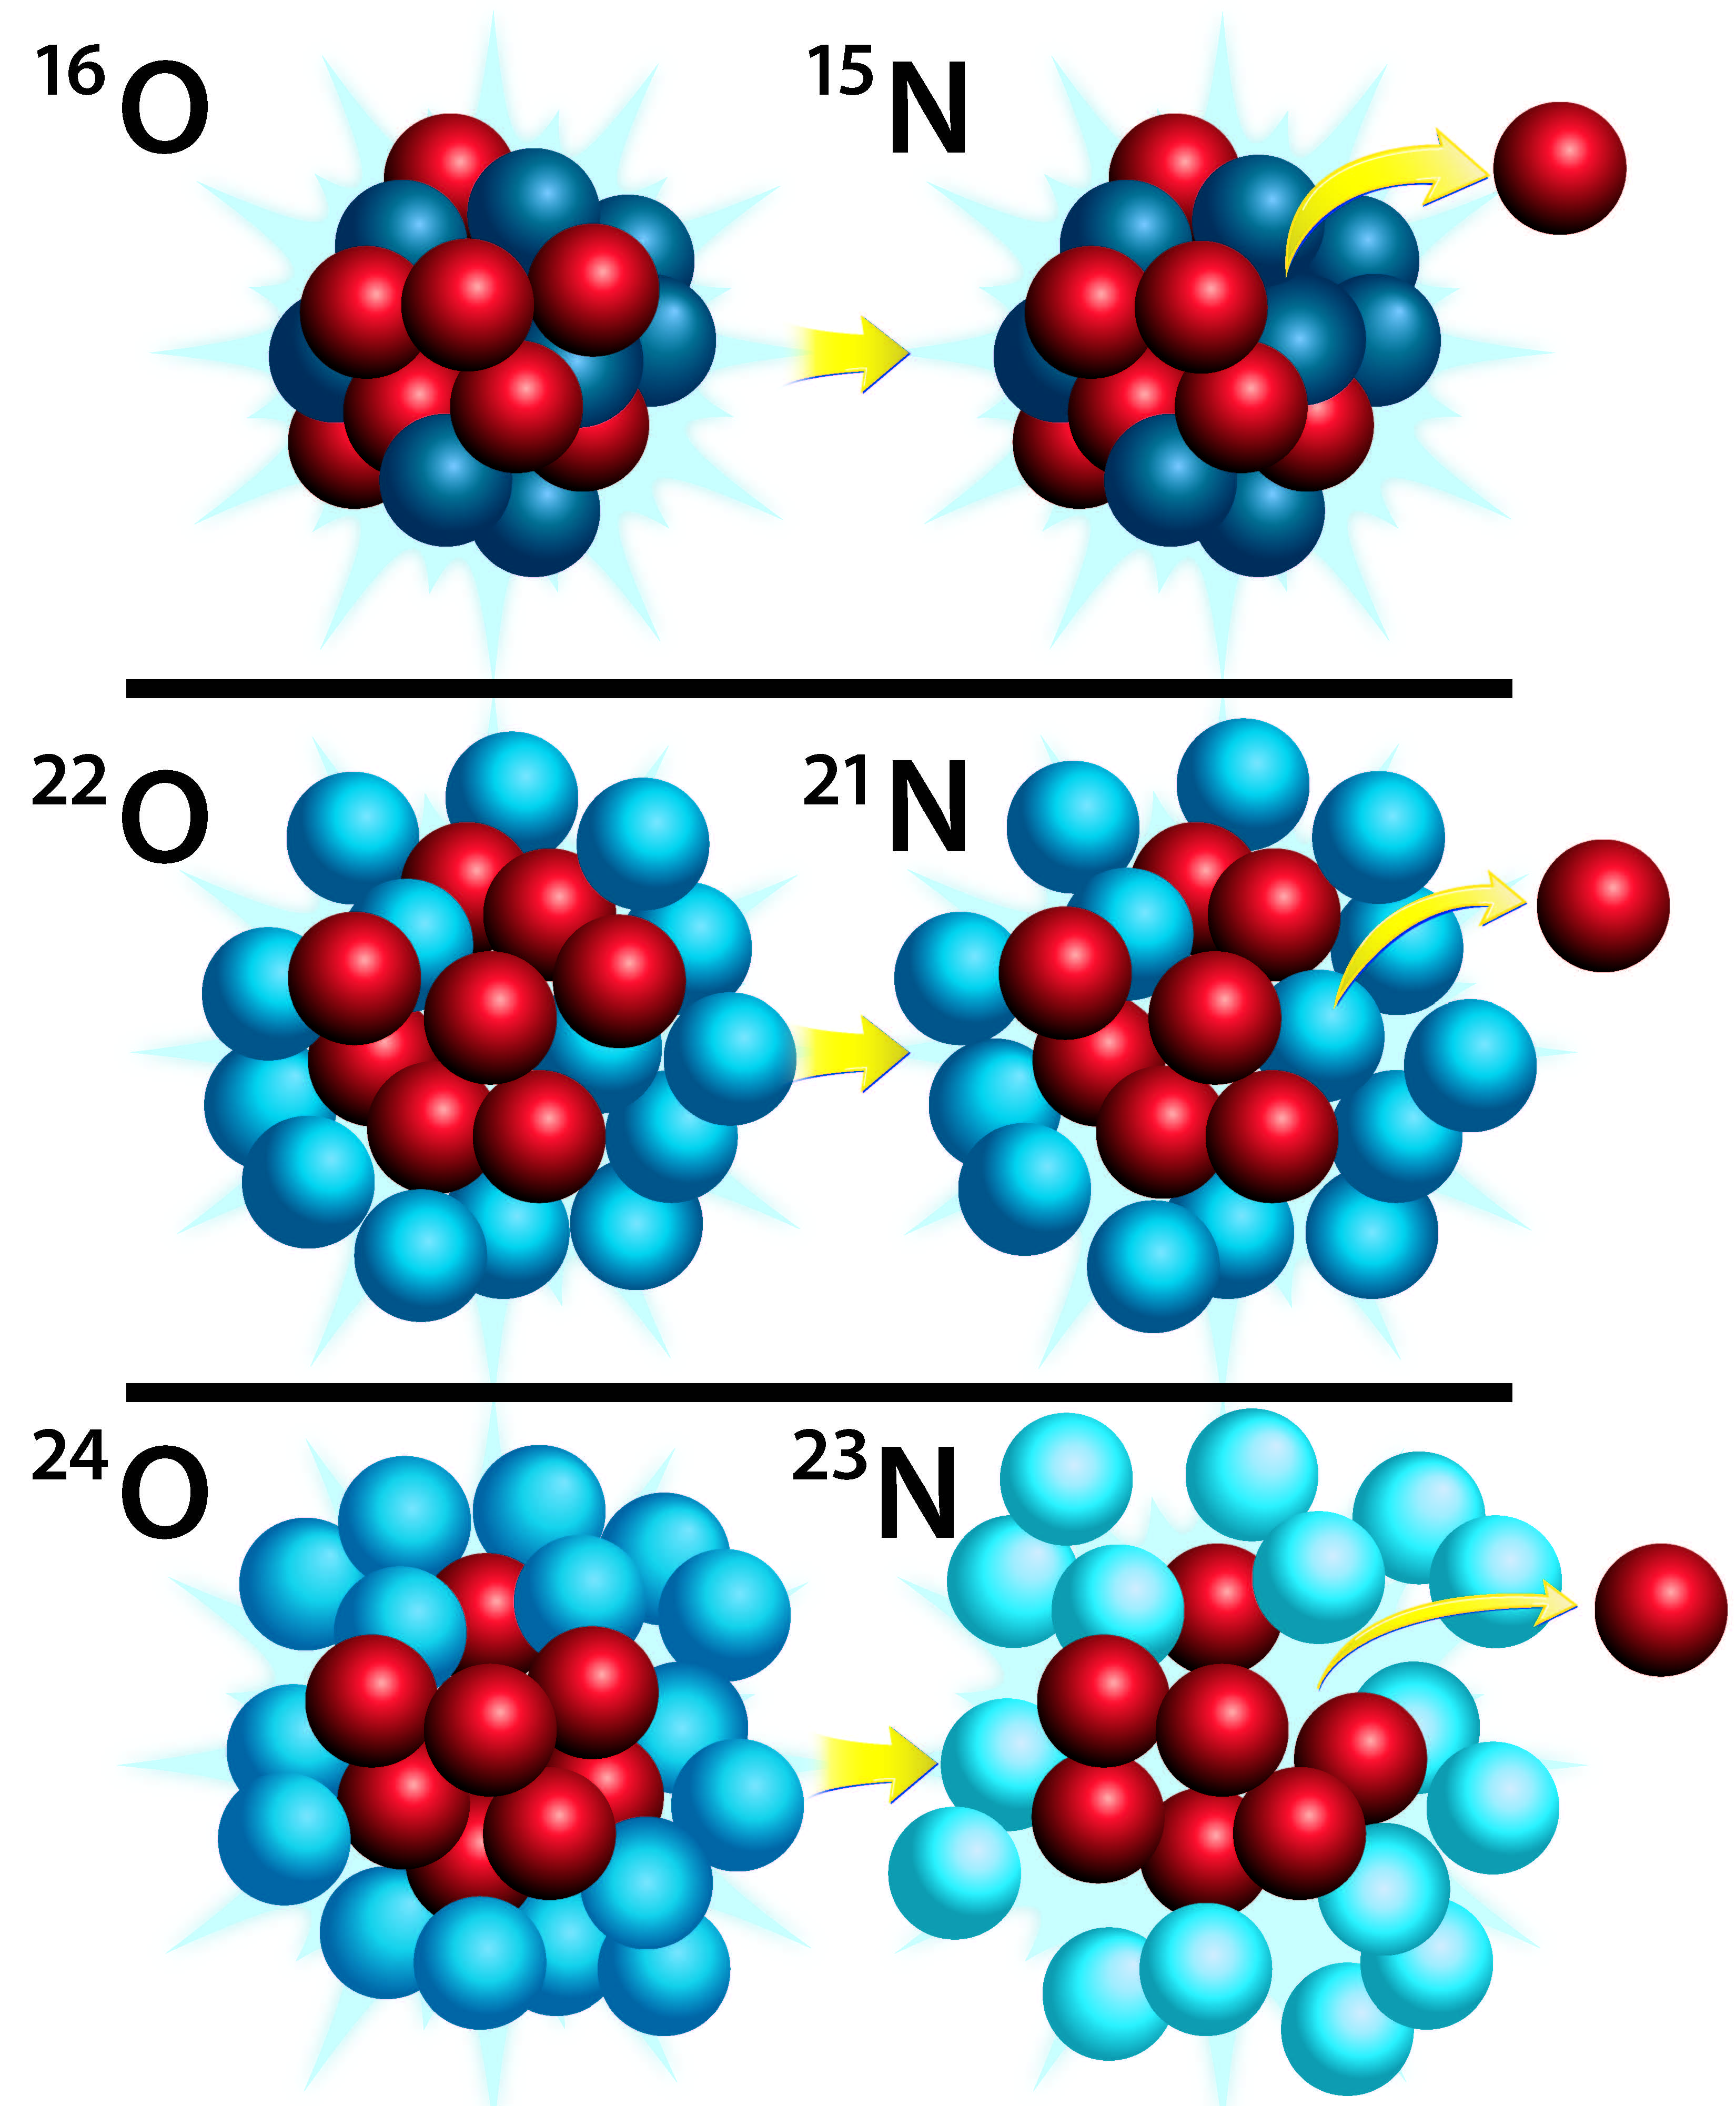
\includegraphics[width=1.2\textwidth]{oxygens.jpg}
      \end{center}
\end{columns}
      \end{footnotesize}
    }


\frame
{
  \frametitle{Recent Articles on Oxygen Isotopes}
  \begin{block}{Many experiments worldwide!}
\begin{itemize}
\item $^{24}$O and lighter:  C.~R.~Hoffman {\em et al.}, Phys.~Lett.~B {\bf 672}, 17 (2009); R.~Kanungo {\em et al.}, Phys.~Rev.~Lett.~{\bf 102}, 152501 (2009);C.~R.~Hoffman {\em et al.}, Phys.~Rev.~C {\bf 83}, 031303(R) (2011);
Stanoiu {\em et al.}, Phys. Rev. C {\bf 69}, 034312 (2004)
\item $^{25}$O: C.~R.~Hoffman {\em et al.}, Phys.~Rev.~Lett.~{\bf 102},152501  (2009). 
\item $^{26}$O: E.~Lunderberg {\it et al.}, Phys.~Rev.~Lett., {\bf 108}, 142503 (2012). 
\item $^{26}$O: Z.~Kohley  {\it et al.}, Study of two-neutron radioactivity in the decay of 26O, Phys.~Rev.~Lett., {\bf 110}, 152501 (2013). 
\item Theory: Oxygen isotopes with three-body forces,  Otsuka {\em et al.},
Phys.~Rev.~Lett., {\bf 105}, 032501  (2010).  
Hagen {\em et al.,} Phys.~Rev.~Lett., {\bf 108}, 242501 (2012). 
\end{itemize}
  \end{block}
}


\frame
    {
      \frametitle{Separation energies and energy gaps for oxygen isotopes}
      \begin{footnotesize}
     \begin{columns}
      \column{5.0cm}
      \begin{center}
	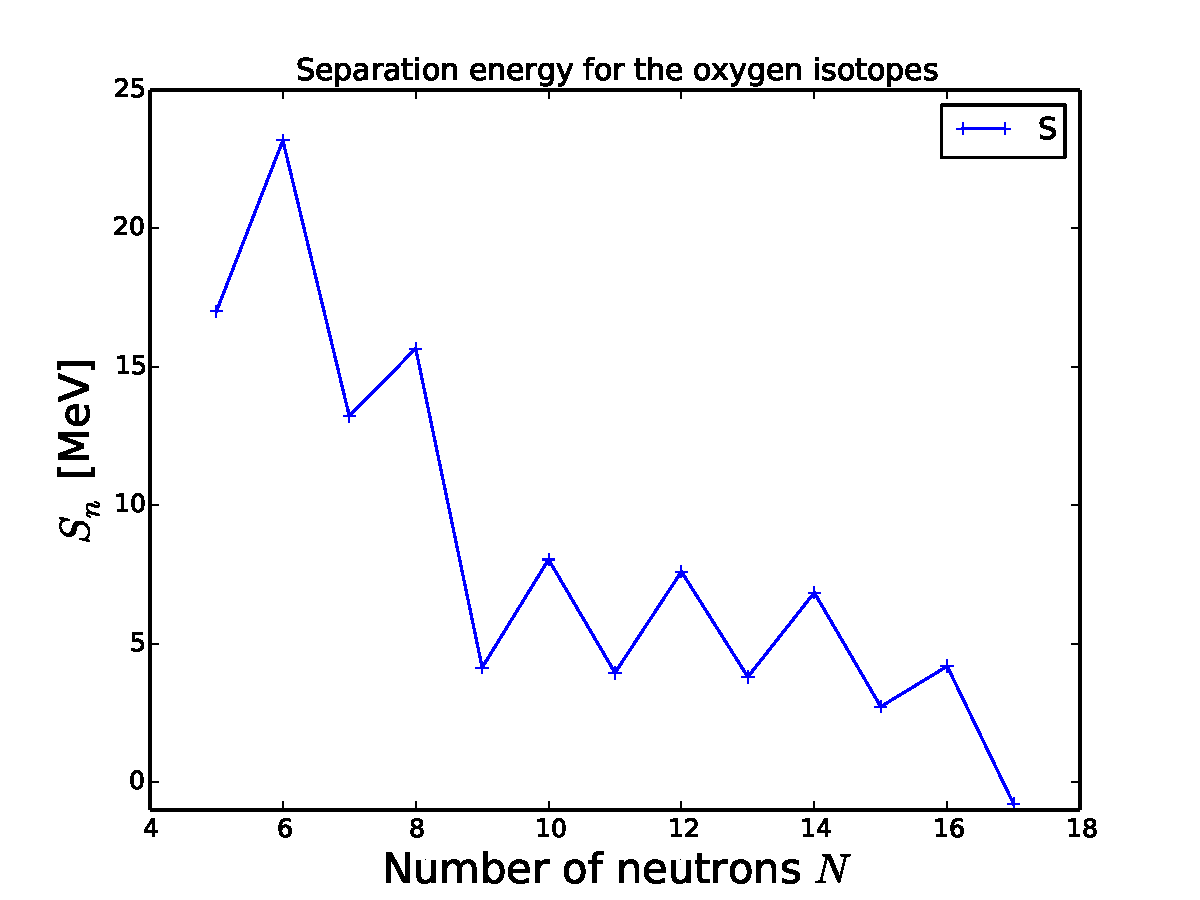
\includegraphics[width=1.2\textwidth]{snoxygen.pdf}
      \end{center}
\column{5cm}
      \begin{center}
	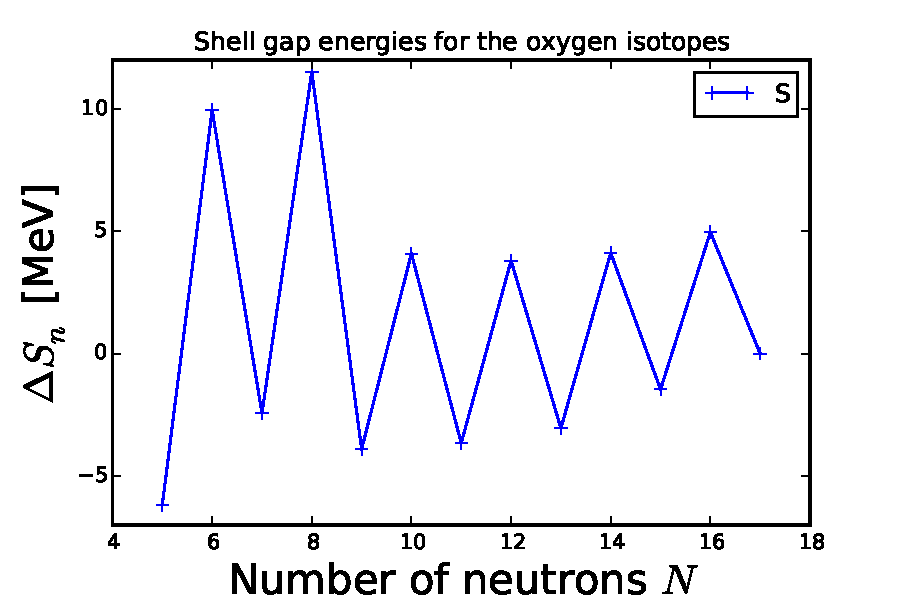
\includegraphics[width=1.2\textwidth]{gapoxygen.pdf}
      \end{center}
\end{columns}
      \end{footnotesize}
    }




\frame
    {
      \frametitle{Calcium isotopes and FRIB plans and capabilities}
      \begin{footnotesize}
     \begin{columns}
      \column{5.0cm}
\begin{itemize}
\item The Ca  isotopes exhibit several possible closed-shell nuclei $^{40}$Ca, $^{48}$Ca, $^{52}$Ca, $^{54}$Ca,
and  $^{60}$Ca. 
\item  Magic neutron numbers are then $N=20, 28, 32, 34, 40$. 
\item Masses available up to $^{54}$Ca, Gallant {\em et al.},Phys.~Rev.~Lett.~{\bf 109}, 032506 (2012) and K.~Baum {\em et al}, Nature {\bf 498}, 346 (2013).
\item Heaviest observed $^{57,58}$Ca. NSCL experiment,  O.~B.~Tarasov {\it et al.}, Phys.~Rev.~Lett.~{\bf 102}, 142501 (2009). Cross sections for $^{59,60}$Ca assumed small ($< 10^{-12}$mb).
\item Which degrees of freedom prevail close to $^{60}$Ca and beyond?
\end{itemize}
\column{6cm}
      \begin{center}
	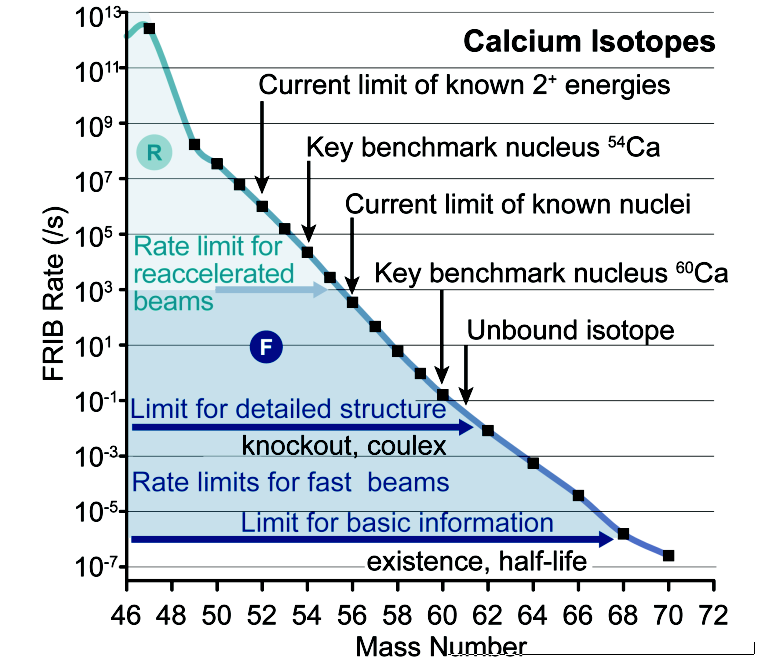
\includegraphics[width=1.15\textwidth]{careach.png}
      \end{center}
\end{columns}
      \end{footnotesize}
    }
\frame
{
  \frametitle{More on Calcium Isotopes}
      \begin{footnotesize}
     \begin{columns}
      \column{5.0cm}
\begin{itemize}
\item {\bf Mass models and mean field models predict the dripline at $A\sim 70$!} Important consequences for modeling of nucleosynthesis related processes.
\item Can we predict reliably which is the last stable calcium isotope? 
\item And how
does this compare with popular mass models on the market? See Nature 486, 509 (2012). 
\item And which parts of the underlying forces
are driving the physics towards the dripline?
\end{itemize}
\column{6cm}
\vspace{-3cm}
      \begin{center}
	\includegraphics[width=1.15\textwidth]{witeknatureca.pdf}
      \end{center}
\end{columns}
      \end{footnotesize}
}
\frame
{
  \frametitle{The calcium isotopes $^{48,52,54,60}$Ca in a naive single-particle picture}
\begin{center}
\setlength{\unitlength}{0.4cm}
\begin{picture}(16,20)
\thicklines
   \put(1,0.5){\makebox(0,0)[bl]{
              \put(0,1){\line(0,1){8}}
              \put(0,9){\line(1,0){8}}
              \put(8,9){\line(0,1){9}}
              \put(8,18){\line(1,0){9}}
              \put(17,1){\line(0,1){17}}
\thinlines
              \put(0.5,2){\line(1,0){7}}
              \put(0.5,4){\line(1,0){7}}
              \put(0.5,6){\line(1,0){7}}
              \put(9.5,6){\line(1,0){7}}
              \put(0.5,11){\line(1,0){7}}
              \put(9.5,4){\line(1,0){7}}
              \put(9.5,2){\line(1,0){7}}
\color{green}
\put(-2,11){\makebox(0,0){$1p0f$}}
\put(-2,6){\makebox(0,0){$1s0d$}}
\put(-2,4){\makebox(0,0){$0p$}}
\put(-2,2){\makebox(0,0){$0s$}}

\color{red}
\put(3,19){\makebox(0,0){$\pi$--protons}}
\put(3,2){\circle*{0.3}}
\put(5,2){\circle*{0.3}}
\put(1.5,4){\circle*{0.3}}
%\put(4,11){\circle*{0.3}}
\put(2.5,4){\circle*{0.3}}
\put(3.5,4){\circle*{0.3}}
\put(4.5,4){\circle*{0.3}}
\put(5.5,4){\circle*{0.3}}
\put(6.5,4){\circle*{0.3}}
\put(1,6){\circle*{0.3}}
\put(1.5,6){\circle*{0.3}}
\put(2,6){\circle*{0.3}}
\put(2.5,6){\circle*{0.3}}
\put(3,6){\circle*{0.3}}
\put(3.5,6){\circle*{0.3}}
\put(4,6){\circle*{0.3}}
\put(4.5,6){\circle*{0.3}}
\put(5,6){\circle*{0.3}}
\put(5.5,6){\circle*{0.3}}
\put(6,6){\circle*{0.3}}
\put(6.5,6){\circle*{0.3}}


\color{blue}
\put(9.5,10){\line(1,0){7}}
\put(12,2){\circle*{0.3}}
\put(14,2){\circle*{0.3}}
\put(10.5,4){\circle*{0.3}}
\put(11.5,4){\circle*{0.3}}
\put(12.5,4){\circle*{0.3}}
\put(13.5,4){\circle*{0.3}}
\put(14.5,4){\circle*{0.3}}
\put(15.5,4){\circle*{0.3}}
\put(10,6){\circle*{0.3}}
\put(10.5,6){\circle*{0.3}}
\put(11,6){\circle*{0.3}}
\put(11.5,6){\circle*{0.3}}
\put(12,6){\circle*{0.3}}
\put(12.5,6){\circle*{0.3}}
\put(13,6){\circle*{0.3}}
\put(13.5,6){\circle*{0.3}}
\put(14,6){\circle*{0.3}}
\put(14.5,6){\circle*{0.3}}
\put(15,6){\circle*{0.3}}
\put(15.5,6){\circle*{0.3}}

\put(11,10){\circle*{0.3}}
\put(11.5,10){\circle*{0.3}}
\put(12,10){\circle*{0.3}}
\put(12.5,10){\circle*{0.3}}
\put(13,10){\circle*{0.3}}
\put(13.5,10){\circle*{0.3}}
\put(14,10){\circle*{0.3}}
\put(14.5,10){\circle*{0.3}}



\put(13,11){\makebox(0,0){$\nu 0f_{7/2}$}}




\put(12,19){\makebox(0,0){$\nu$--neutrons}}
%\put(-1.0,14){\makebox(0,0){\alert{$\Delta \epsilon^{\pi}_{j_a}\propto\sum_{j_i\le F}\overline{v}_{j_aj_i}\normord{a^\dagger_a a_i}$}}}
\pause
              \put(9.5,12){\line(1,0){7}}
\put(13,13){\makebox(0,0){$\nu 1p_{3/2}$}}
\put(10.5,12){\circle*{0.3}}
\put(12.25,12){\circle*{0.3}}
\put(14,12){\circle*{0.3}}
\put(15.75,12){\circle*{0.3}}

\pause
\put(13,15){\makebox(0,0){$\nu 1p_{1/2}$}}
              \put(9.5,14){\line(1,0){7}}
\put(12,14){\circle*{0.3}}
\put(14,14){\circle*{0.3}}

\pause
              \put(9.5,16){\line(1,0){7}}
\put(13,17){\makebox(0,0){$\nu 0f_{5/2}$}}
\put(10.5,16){\circle*{0.3}}
\put(11.5,16){\circle*{0.3}}
\put(12.5,16){\circle*{0.3}}
\put(13.5,16){\circle*{0.3}}
\put(14.5,16){\circle*{0.3}}
\put(15.5,16){\circle*{0.3}}




         }}
\end{picture}
\end{center}
}


\frame
    {
      \frametitle{Separation energies and energy gaps for calcium isotopes}
      \begin{footnotesize}
     \begin{columns}
      \column{5.0cm}
      \begin{center}
	\includegraphics[width=1.2\textwidth]{sncalcium.pdf}
      \end{center}
\column{5cm}
      \begin{center}
	\includegraphics[width=1.2\textwidth]{gapcalcium.pdf}
      \end{center}
\end{columns}
      \end{footnotesize}
    }


\frame
    {
      \frametitle{Other chains of isotopes of crucial interest for FRIB like physics: nickel isotopes}
      \begin{footnotesize}
     \begin{columns}
      \column{5.0cm}
\begin{itemize}
\item This chain of isotopes exhibits four possible closed-shell nuclei $^{48}$Ni, $^{56}$Ni, $^{68}$Ni
and  $^{78}$Ni.  {\bf FRIB plans systematic studies from $^{48}$Ni to $^{88}$Ni.}
\item  Neutron skin possible for $^{84}$Ni at FRIB.
\item Which is the best closed-shell nucleus?
And again, which part of the nuclear forces drives it?  Is it the strong spin-orbit force, the tensor force, or ..?
\end{itemize}
\column{5cm}
      \begin{center}
\setlength{\unitlength}{0.3cm}
\begin{picture}(16,20)
\thicklines
   \put(1,0.5){\makebox(0,0)[bl]{
              \put(0,1){\line(0,1){8}}
              \put(0,9){\line(1,0){8}}
              \put(8,9){\line(0,1){9}}
              \put(8,18){\line(1,0){9}}
              \put(17,1){\line(0,1){17}}
\thinlines
              \put(0.5,2){\line(1,0){7}}
              \put(0.5,4){\line(1,0){7}}
              \put(0.5,6){\line(1,0){7}}
              \put(9.5,6){\line(1,0){7}}
              \put(9.5,8){\line(1,0){7}}
              \put(0.5,12){\line(1,0){7}}
              \put(0.5,8){\line(1,0){7}}
              \put(9.5,4){\line(1,0){7}}
              \put(9.5,2){\line(1,0){7}}
\color{green}
\put(-0.5,11){\makebox(0,0){$1p0f_{5/2}0g_{9/2}$}}
\put(-2,8){\makebox(0,0){$0f_{7/2}$}}
\put(-2,6){\makebox(0,0){$1s0d$}}
\put(-2,4){\makebox(0,0){$0p$}}
\put(-2,2){\makebox(0,0){$0s$}}

\color{red}
\put(3,19){\makebox(0,0){$\pi$--protons}}
\put(3,2){\circle*{0.3}}
\put(5,2){\circle*{0.3}}
\put(1.5,4){\circle*{0.3}}
\put(2.5,4){\circle*{0.3}}
\put(3.5,4){\circle*{0.3}}
\put(4.5,4){\circle*{0.3}}
\put(5.5,4){\circle*{0.3}}
%\put(4,12){\circle*{0.3}}
\put(6.5,4){\circle*{0.3}}
\put(1,6){\circle*{0.3}}
\put(1.5,6){\circle*{0.3}}
\put(2,6){\circle*{0.3}}
\put(2.5,6){\circle*{0.3}}
\put(3,6){\circle*{0.3}}
\put(3.5,6){\circle*{0.3}}
\put(4,6){\circle*{0.3}}
\put(4.5,6){\circle*{0.3}}
\put(5,6){\circle*{0.3}}
\put(5.5,6){\circle*{0.3}}
\put(6,6){\circle*{0.3}}
\put(6.5,6){\circle*{0.3}}
\put(2,8){\circle*{0.3}}
\put(2.5,8){\circle*{0.3}}
\put(3,8){\circle*{0.3}}
\put(3.5,8){\circle*{0.3}}
\put(4,8){\circle*{0.3}}
\put(4.5,8){\circle*{0.3}}
\put(5,8){\circle*{0.3}}
\put(5.5,8){\circle*{0.3}}


\color{blue}
\put(9.5,10){\line(1,0){7}}
\put(12,2){\circle*{0.3}}
\put(14,2){\circle*{0.3}}
\put(10.5,4){\circle*{0.3}}
\put(11.5,4){\circle*{0.3}}
\put(12.5,4){\circle*{0.3}}
\put(13.5,4){\circle*{0.3}}
\put(14.5,4){\circle*{0.3}}
\put(15.5,4){\circle*{0.3}}
\put(10,6){\circle*{0.3}}
\put(10.5,6){\circle*{0.3}}
\put(11,6){\circle*{0.3}}
\put(11.5,6){\circle*{0.3}}
\put(12,6){\circle*{0.3}}
\put(12.5,6){\circle*{0.3}}
\put(13,6){\circle*{0.3}}
\put(13.5,6){\circle*{0.3}}
\put(14,6){\circle*{0.3}}
\put(14.5,6){\circle*{0.3}}
\put(15,6){\circle*{0.3}}
\put(15.5,6){\circle*{0.3}}

\put(11,8){\circle*{0.3}}
\put(11.5,8){\circle*{0.3}}
\put(12,8){\circle*{0.3}}
\put(12.5,8){\circle*{0.3}}
\put(13,8){\circle*{0.3}}
\put(13.5,8){\circle*{0.3}}
\put(14,8){\circle*{0.3}}
\put(14.5,8){\circle*{0.3}}
\put(12,19){\makebox(0,0){$\nu$--neutrons}}






\pause

              \put(9.5,10){\line(1,0){7}}
\put(13,11){\makebox(0,0){$\nu 1p_{3/2}$}}
\put(10.5,10){\circle*{0.3}}
\put(12.25,10){\circle*{0.3}}
\put(14,10){\circle*{0.3}}
\put(15.75,10){\circle*{0.3}}


\put(13,13){\makebox(0,0){$\nu 1p_{1/2}$}}
              \put(9.5,12){\line(1,0){7}}
\put(12,12){\circle*{0.3}}
\put(14,12){\circle*{0.3}}

              \put(9.5,14){\line(1,0){7}}
\put(13,15){\makebox(0,0){$\nu 0f_{5/2}$}}
\put(10.5,14){\circle*{0.3}}
\put(11.5,14){\circle*{0.3}}
\put(12.5,14){\circle*{0.3}}
\put(13.5,14){\circle*{0.3}}
\put(14.5,14){\circle*{0.3}}
\put(15.5,14){\circle*{0.3}}
\pause
\put(13,17){\makebox(0,0){$\nu 0g_{9/2}$}}
              \put(9.5,16){\line(1,0){7}}
\put(10.5,16){\circle*{0.3}}
\put(11,16){\circle*{0.3}}
\put(11.5,16){\circle*{0.3}}
\put(12,16){\circle*{0.3}}
\put(12.5,16){\circle*{0.3}}
\put(13,16){\circle*{0.3}}
\put(13.5,16){\circle*{0.3}}
\put(14,16){\circle*{0.3}}
\put(14.5,16){\circle*{0.3}}
\put(15,16){\circle*{0.3}}

         }}
\end{picture}

      \end{center}
\end{columns}
      \end{footnotesize}
    }

\frame
    {
      \frametitle{Separation energies and energy gaps for nickel isotopes}
      \begin{footnotesize}
     \begin{columns}
      \column{5.0cm}
      \begin{center}
	\includegraphics[width=1.2\textwidth]{snnickel.pdf}
      \end{center}
\column{5cm}
      \begin{center}
	\includegraphics[width=1.2\textwidth]{gapnickel.pdf}
      \end{center}
\end{columns}
      \end{footnotesize}
    }

\frame
{
  \frametitle{Tin isotopes}

  \begin{block}{From $^{100}$Sn to nuclei beyond $^{132}$Sn}
\begin{enumerate}
\item $^{137}$Sn is the last reported neutron-rich isotope (with half-life).
\item To understand which parts of the nuclear Hamiltonian that drives the
properties of such nuclei will be crucial for our understanding of the stability of matter.
\item Zr isotopes form also long chains of neutron-rich isotopes. {\bf FRIB plans from $^{80}$Zr to
$^{120}$Zr.}
\item And why neutron rich isotopes? {\bf Here the possibility to constrain nuclear forces from in-medium results.}
\end{enumerate}
  \end{block}
 }  

\frame
    {
      \frametitle{Separation energies and energy gaps for tin isotopes}
      \begin{footnotesize}
     \begin{columns}
      \column{5.0cm}
      \begin{center}
	\includegraphics[width=1.2\textwidth]{sntin.pdf}
      \end{center}
\column{5cm}
      \begin{center}
	\includegraphics[width=1.2\textwidth]{gaptin.pdf}
      \end{center}
\end{columns}
      \end{footnotesize}
    }


\frame
    {
      \frametitle{Finally, separation energies and energy gaps for lead isotopes}
      \begin{footnotesize}
     \begin{columns}
      \column{5.0cm}
      \begin{center}
	\includegraphics[width=1.2\textwidth]{snlead.pdf}
      \end{center}
\column{5cm}
      \begin{center}
	\includegraphics[width=1.2\textwidth]{gaplead.pdf}
      \end{center}
\end{columns}
      \end{footnotesize}
    }

\frame
{
  \frametitle{Brief summary}

  \begin{block}{Features to be noted}
Since we will focus in the beginning on single-particle degrees of freedom and mean-field approaches before we
start with nuclear forces and many-body approaches like the nuclear shell-model, there are some features to be noted
\begin{enumerate}
\item  The total binding energy is not that different from the sum of the individual neutron and proton masses. 
One may thus infer that intrinsic properties of nucleons in a nucleus are close to those of free nucleons.
\item We note clearly a staggering effect between odd and even isotopes with the even ones being more bound (larger separation energies). We will later link this to strong pairing correlations in nuclei.
\item We note also that there are large shell-gaps for some nuclei, meaning that more energy is needed to remove one nucleon. These gaps are used to define so-called magic numbers. 
\end{enumerate}
  \end{block}
 }  



\frame
{
  \frametitle{Radii}
\begin{small}
{\scriptsize
The root-mean-square (rms) charge radius has been measured for the ground states of many
nuclei. For a spherical charge density, $\rho({\bf r})$, the mean-square radius is defined by:
\[
\langle r^2\rangle = \frac{ \int  d {\bf r} \rho({\bf r}) r^2}{ \int  d {\bf r} \rho({\bf r})},
\]
and the rms radius is the square root of this quantity denoted by
\[
R =\sqrt{ \langle r^2\rangle}.
\]
}
\end{small}
}

\frame
{
  \frametitle{Radii}
\begin{small}
{\scriptsize

Radii for most stable
nuclei have been deduced from electron scattering form
factors and/or from the x-ray transition energies of muonic atoms. 
The relative radii for a
series of isotopes can be extracted from the isotope shifts of atomic x-ray transitions.
The rms radius for the nuclear point-proton density, $R_p$ is obtained from the rms charge radius by:
\[
R_p = \sqrt{R^2_{\mathrm{ch}}- R^2_{\mathrm{corr}}},
\]
where
\[
R^2_{\mathrm{corr}}= R^2_{\mathrm{op}}+(N/Z)R^2_{\mathrm{on}}+R^2_{\mathrm{rel}},
\]
where $ R_{\mathrm{op}}= 0.875(7)$ fm  is the rms radius of the proton, $R^2_{\mathrm{on}} = 0.116(2)$ fm$^2$ is the
mean-square radius of the neutron and $R^2_{\mathrm{rel}} = 0.033$ fm$^2$ is the relativistic Darwin-Foldy correction. There are also smaller nucleus-dependent relativistic spin-orbit and
mesonic-exchange corrections that should be included.
}
\end{small}
}


\frame
{
\frametitle{Definitions}
An operator is defined as $\hat{O}$ throughout. Unless otherwise
specified the number of particles is always $A$ and $d$ is the dimension of the 
system. 
In nuclear physics we normally define the total number of particles to be $A=N+Z$,
where $N$ is total number of neutrons and $Z$ the total number of protons. In case of other baryons such isobars $\Delta$ or
various hyperons such as $\Lambda$ or $\Sigma$, one needs to add their definitions.  
%
Hereafter, $A$ is reserved for the total number of particles, unless otherwise specificied. When we refer to a neutron we will use the label $n$ and when we refer to a proton we will use the label $p$. Unless otherwise specified, we will call these particles for nucleons.
}



\frame
{
\frametitle{Definitions}
The quantum numbers of a single-nucleon state in coordinate space are
defined by the variable $x=({\bf r},\sigma)$, where ${\bf r}\in {\mathbb{R}}^{d}$with $d=1,2,3$ represents the spatial coordinates and $\sigma$ is the eigenspin of the nucleon. For fermions with eigenspin $1/2$ this means that
\[
 x\in {\mathbb{R}}^{d}\oplus (\frac{1}{2}),
\]
and the integral
\[
\int dx = \sum_{\sigma}\int d^dr = \sum_{\sigma}\int d{\bf r},
\]
and
\[
\int d^Ax= \int dx_1\int dx_2\dots\int dx_A.
\]

}


\frame
{
\frametitle{Definitions}
The quantum mechanical wave function of a given state with quantum numbers $\lambda$ (encompassing all quantum numbers needed to specify the system), ignoring time, is
\[
\Psi_{\lambda}=\Psi_{\lambda}(x_1,x_2,\dots,x_A),
\]
with $x_i=({\bf r}_i,\sigma_i)$ and the projection of $\sigma_i$ takes the values
$\{-1/2,+1/2\}$ for nucleons with spin $1/2$. 
We will hereafter always refer to $\Psi_{\lambda}$ as the exact wave function, and if the ground state is not degenerate we label it as 
\[
\Psi_0=\Psi_0(x_1,x_2,\dots,x_A).
\]

}


\frame
{
\frametitle{Definitions}
Since the solution $\Psi_{\lambda}$ seldomly can be found in closed form, approximations are sought. In this text we define an approximative wave function or an ansatz to the exact wave function as 
\[
\Phi_{\lambda}=\Phi_{\lambda}(x_1,x_2,\dots,x_A),
\]
with 
\[
\Phi_0=\Phi_0(x_1,x_2,\dots,x_A),
\]
being the ansatz to the ground state.  
}


\frame
{
\frametitle{Definitions}
The wave function $\Psi_{\lambda}$ is sought in the Hilbert space of either symmetric or anti-symmetric $A$-body functions, namely
\[
\Psi_{\lambda}\in {\cal H}_A:= {\cal H}_1\oplus{\cal H}_1\oplus\dots\oplus{\cal H}_1,
\]
where the single-nucleon Hilbert space ${\cal H}_1$ is the space of square integrable functions over
$\in {\mathbb{R}}^{d}\oplus (\sigma)$
resulting in
\[
{\cal H}_1:= L^2(\mathbb{R}^{d}\oplus (\sigma)).
\]
}

\section[Week 3]{Week 3}

\frame
{
  \frametitle{Topics for Week 3, January 13-17}
  \begin{block}{Single-particle fields and construction of many-body wave functions}
\begin{itemize}
\item Monday:
\item Repetition from last week
\item Hamiltonians and single-particle fields, continued from last week
\item Further discussion of basis functions and mentioning the Woods-Saxon potential (AB chapter 10 and JS chapter 3)
\item Wednesday:
\item Hamiltonians and single-particle fields and start Hartree-Fock theory
\item Friday: Discussion of exercises 1 and 2. Demonstrations (computational topics).
\end{itemize}
Suggested literature is AB chapters 9-11 and 14 and JS chapter 3 and 4
  \end{block}
} 



\frame
{
  \frametitle{Liquid drop model as a simple parametrization of binding energies}
  \begin{block}{Explaining the various terms}
For the liquid drop model we have
\[ BE(N,Z) = a_1A-a_2A^{2/3}-a_3\frac{Z^2}{A^{1/3}}-a_4\frac{(N-Z)^2}{A}\]
We could also add a so-called pairing term, which is a correction term that
arises from the tendency of proton pairs and neutron pairs to
occur. An even number of particles is more stable than an odd number.
\begin{itemize}
\item $a_1A$: Volume energy. When an assembly of nucleons of the same size is packed
together into the smallest volume, each interior nucleon has a certain
number of other nucleons in contact with it. This contribution is proportional to the volume.
\end{itemize}

  \end{block}
} 

\frame
{
  \frametitle{More on the liquid drop model}
  \begin{block}{Explaining the various terms}
\begin{itemize}
\item $a_2A^{2/3}$:   Surface energy. A nucleon at the
surface of a nucleus interacts with fewer other nucleons than one in
the interior of the nucleus and hence its binding energy is less. This
surface energy term takes that into account and is therefore negative
and is proportional to the surface area.
\item $a_3\frac{Z^2}{A^{1/3}}$: Coulomb Energy. The electric
repulsion between each pair of protons in a nucleus yields less binding. 
\item $a_4\frac{(N-Z)^2}{A}$: Asymmetry energy, associated with the Pauli exclusion principle 
and reflecting the fact that the proton-neutron interaction is more attractive on the average than the neutron-neutron and proton-proton interactions.
\end{itemize}

  \end{block}
} 


\frame
    {
      \frametitle{Binding energies and the liquid drop model}
      \begin{footnotesize}
\[ BE(N,Z) = a_1A-a_2A^{2/3}-a_3\frac{Z^2}{A^{1/3}}-a_4\frac{(N-Z)^2}{A}\]
     \begin{columns}
      \column{5.0cm}
\begin{itemize}
\item Red: experimental data, blue: liquid drop model
\item $a_1=15.49$ MeV
\item $a_2=17.23$ MeV
\item $a_3=0.697$ MeV
\item $a_4=22.6$ MeV
\end{itemize}
\column{5cm}
      \begin{center}
	\includegraphics[width=1.2\textwidth]{beexpliquid.pdf}
      \end{center}
\end{columns}
      \end{footnotesize}
    }



\frame
{
\frametitle{Definitions}
Our Hamiltonian is invariant under the permutation (interchange) of two nucleons.
Since we deal with fermions however, the total wave function is antisymmetric.
Let $\hat{P}$ be an operator which interchanges two nucleons.
Due to the symmetries we have ascribed to our Hamiltonian, this operator commutes with the total Hamiltonian,
\[
[\hat{H},\hat{P}] = 0,
\]
meaning that $\Psi_{\lambda}(x_1, x_2, \dots , x_A)$ is an eigenfunction of 
$\hat{P}$ as well, that is
\[
\hat{P}_{ij}\Psi_{\lambda}(x_1, x_2, \dots,x_i,\dots,x_j,\dots,x_A)=
\beta\Psi_{\lambda}(x_1, x_2, \dots,x_j,\dots,x_i,\dots,x_A),
\]
where $\beta$ is the eigenvalue of $\hat{P}$. We have introduced the suffix $ij$ in order to indicate that we permute nucleons $i$ and $j$.
The Pauli principle tells us that the total wave function for a system of fermions
has to be antisymmetric, resulting in the eigenvalue $\beta = -1$.   

}

\frame
{
  \frametitle{Definitions and notations}
\begin{small}
{\scriptsize
The Schr\"odinger equation reads 
\begin{equation}
\hat{H}(x_1, x_2, \dots , x_A) \Psi_{\lambda}(x_1, x_2, \dots , x_A) = 
E_\lambda  \Psi_\lambda(x_1, x_2, \dots , x_A), 
\label{eq:basicSE1}
\end{equation}
where the vector $x_i$ represents the coordinates (spatial and spin) of nucleon $i$, $\lambda$ stands  for all the quantum
numbers needed to classify a given $A$-nucleon state and $\Psi_{\lambda}$ is the pertaining eigenfunction.  Throughout this course,
$\Psi$ refers to the exact eigenfunction, unless otherwise stated.
}
\end{small}
}

\frame
{
  \frametitle{Definitions and notations}
\begin{small}
{\scriptsize
We write the Hamilton operator, or Hamiltonian,  in a generic way 
\[
	\hat{H} = \hat{T} + \hat{V} 
\]
where $\hat{T}$  represents the kinetic energy of the system
\[
	\hat{T} = \sum_{i=1}^A \frac{\mathbf{p}_i^2}{2m_i} = \sum_{i=1}^A \left( -\frac{\hbar^2}{2m_i} \mathbf{\nabla_i}^2 \right) =
		\sum_{i=1}^A t(x_i)
\]
while the operator $\hat{V}$ for the potential energy is given by
\begin{equation}
	\hat{V} = \sum_{i=1}^A \hat{u}_{\mathrm{ext}}(x_i) + \sum_{ji=1}^A v(x_i,x_j)+\sum_{ijk=1}^Av(x_i,x_j,x_k)+\dots
\label{eq:firstv}
\end{equation}
Hereafter we use natural units, viz.~$\hbar=c=e=1$, with $e$ the elementary charge and $c$ the speed of light. This means that momenta and masses
have dimension energy. 
}
\end{small}
}
\frame
{
  \frametitle{Definitions and notations}
\begin{small}
{\scriptsize
If one does quantum chemistry, after having introduced the  Born-Oppenheimer approximation which effectively freezes out the nucleonic degrees
of freedom, the Hamiltonian for $N=n_e$ electrons takes the following form 
\[
  \hat{H} = \sum_{i=1}^{n_e} t(x_i) 
  - \sum_{i=1}^{n_e} k\frac{Z}{r_i} + \sum_{i<j}^{n_e} \frac{k}{r_{ij}},
\]
with $k=1.44$ eVnm
}
\end{small}
}

\frame
{
  \frametitle{Definitions and notations}
\begin{small}
{\scriptsize
 We can rewrite this as
\begin{equation}
    \hat{H} = \hat{H_0} + \hat{H_I} 
    = \sum_{i=1}^{n_e}\hat{h}_0(x_i) + \sum_{i<j=1}^{n_e}\frac{1}{r_{ij}},
\label{H1H2}
\end{equation}
where  we have defined $r_{ij}=| {\bf r}_i-{\bf r}_j|$ and
\begin{equation}
  \hat{h}_0(x_i) =  \hat{t}(x_i) - \frac{Z}{x_i}.
\label{hi}
\end{equation}
The first term of eq.~(\ref{H1H2}), $H_0$, is the sum of the $N$
\emph{one-body} Hamiltonians $\hat{h}_0$. Each individual
Hamiltonian $\hat{h}_0$ contains the kinetic energy operator of an
electron and its potential energy due to the attraction of the
nucleus. The second term, $H_I$, is the sum of the $n_e(n_e-1)/2$
two-body interactions between each pair of electrons. Note that the double sum carries a restriction $i<j$.
}
\end{small}
}

\frame
{
  \frametitle{Definitions and notations}
\begin{small}
{\scriptsize
The potential energy term due to the attraction of the nucleus defines the one-body field $u_i=u_{\mathrm{ext}}(x_i)$ of Eq.~(\ref{eq:firstv}).
We have moved this term into the $\hat{H}_0$ part of the Hamiltonian, instead of keeping  it in $\hat{V}$ as in  Eq.~(\ref{eq:firstv}).
The reason is that we will hereafter treat $\hat{H}_0$ as our non-interacting  Hamiltonian. For a many-body wavefunction $\Phi_{\lambda}$ defined by an  
appropriate single-nucleon basis, we may solve exactly the non-interacting eigenvalue problem 
\[
\hat{H}_0\Phi_{\lambda}= w_{\lambda}\Phi_{\lambda},
\]
with $w_{\lambda}$ being the non-interacting energy. This energy is defined by the sum over single-nucleon energies to be defined below.
For atoms the single-nucleon energies could be the hydrogen-like single-nucleon energies corrected for the charge $Z$. For nuclei and quantum
dots, these energies could be given by the harmonic oscillator in three and two dimensions, respectively.
}
\end{small}
}

\frame
{
  \frametitle{Definitions and notations}
\begin{small}
{\scriptsize
We will assume that the interacting part of the Hamiltonian
can be approximated by a two-body interaction.
This means that our Hamiltonian is written as 
\begin{equation}
    \hat{H} = \hat{H_0} + \hat{H_I} 
    = \sum_{i=1}^A \hat{h}_0(x_i) + \sum_{i<j=1}^A \hat{v}(x_{ij}),
\label{Hnuclei}
\end{equation}
with 
\begin{equation}
  H_0=\sum_{i=1}^A \hat{h}_0(x_i) =  \sum_{i=1}^A\left(\hat{t}(x_i) + \hat{u}_{\mathrm{ext}}(x_i)\right).
\label{hinuclei}
\end{equation}
The one-body part $u_{\mathrm{ext}}(x_i)$ is normally approximated by a harmonic oscillator potential or the Coulomb interaction an electron feels from the nucleus. However, other potentials are fully possible, such as 
one derived from the self-consistent solution of the Hartree-Fock equations or so-called Woods-Saxon potentials to be discussed this week (and later in this course).
}
\end{small}
}

\frame
{
  \frametitle{The Woods-Saxon potential}
\begin{small}
{\scriptsize
We have defined
\[
    \hat{H} = \hat{H_0} + \hat{H_I} 
    = \sum_{i=1}^A \hat{h}_0(x_i) + \sum_{i<j=1}^A \hat{v}(x_{ij}),
\]
with 
\[
  H_0=\sum_{i=1}^A \hat{h}_0(x_i) =  \sum_{i=1}^A\left(\hat{t}(x_i) + \hat{u}_{\mathrm{ext}}(x_i)\right).
\]

In nuclear physics the one-body part $u_{\mathrm{ext}}(x_i)$ is often approximated by a harmonic oscillator potential or a
Woods-Saxon potential. However, this is not fully correct, because as we have discussed, nuclei are self-bound systems and there is no external confining potential. {\bf The Hamiltonian $H_0$ cannot be used to compute the binding energy of a nucleus since it is not based on a model for the nuclear forces.}. That is, the binding energy is not the sum of the individual single-particle energies. 
}
\end{small}
}


\frame
{
  \frametitle{The Woods-Saxon potential}
\begin{small}
{\scriptsize
The Woods-Saxon potential is a mean field potential for the nucleons (protons and neutrons) 
inside an atomic nucleus. It represent an average potential that a given nucleon feels from  the forces applied on each nucleon. 
The parametrization is
\[
\hat{u}_{\mathrm{ext}}(r)=-\frac{V_0}{1+\exp{(r-R)/a}},
\]
with $V_0\approx 50$ MeV representing the potential well depth, $a\approx 0.5$ fm 
length representing the "surface thickness" of the nucleus and $R=r_0A^{1/3}$, with $r_0=1.25$ fm and $A$ the number of nucleons.
The value for $r_0$ can be extracted from a fit to data, see for example M.~Kirson, Nucl.~Phys.~A {\bf 781}, 350 (2007).
}
\end{small}
}


\frame
    {
      \frametitle{The Woods-Saxon potential}
      \begin{footnotesize}
     \begin{columns}
      \column{4.0cm}
\begin{itemize}
\item It rapidly approaches zero as $r$ goes to infinity, reflecting the short-distance nature of the strong nuclear force.
\item For large $A$, it is approximately flat in the center.
\item Nucleons near the surface of the nucleus experience a large force towards the center.
\end{itemize}
\column{6cm}
      \begin{center}
	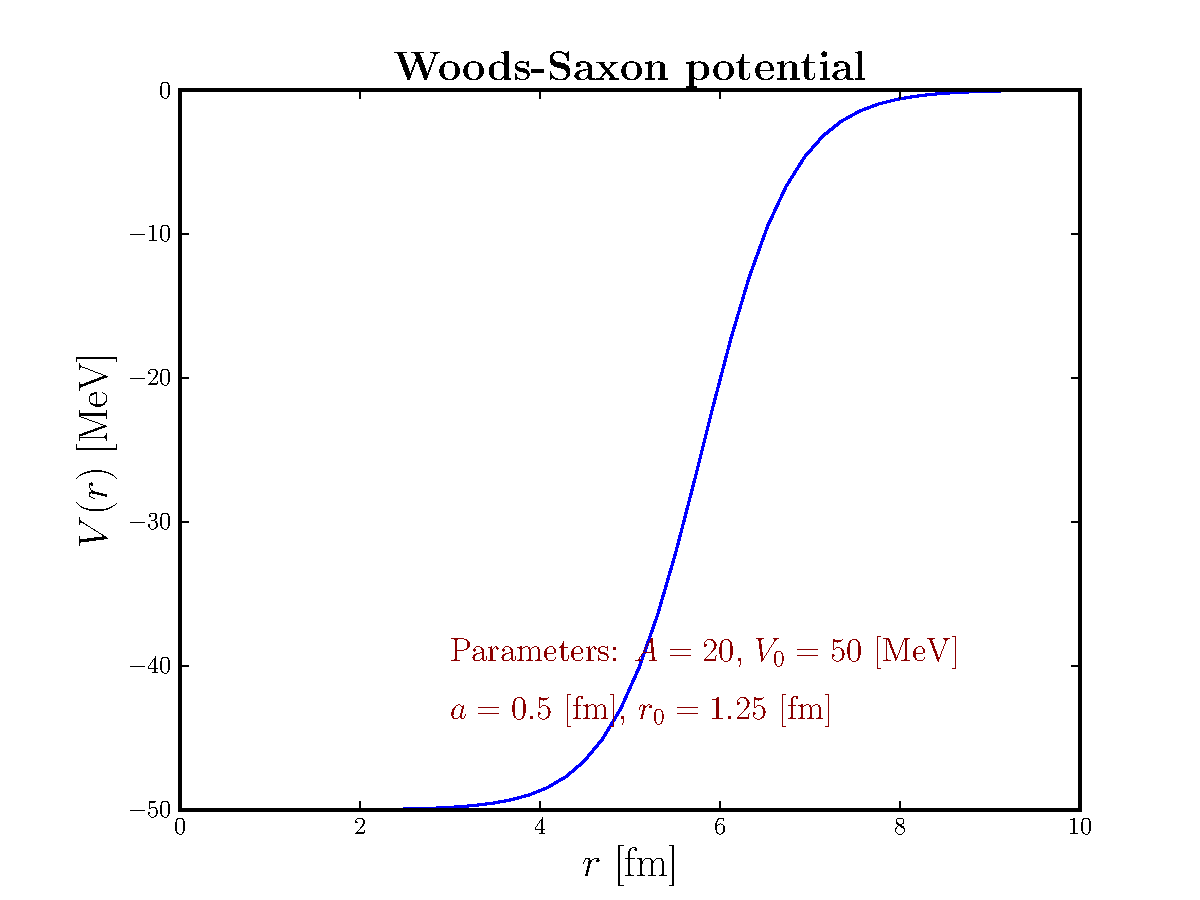
\includegraphics[width=1.25\textwidth]{woodsaxon.pdf}
      \end{center}
\end{columns}
      \end{footnotesize}
    }


\frame
{
  \frametitle{The harmonic oscillator Hamiltonian}
\begin{small}
{\scriptsize
We have defined
\[
    \hat{H} = \hat{H_0} + \hat{H_I} 
    = \sum_{i=1}^A \hat{h}_0(x_i) + \sum_{i<j=1}^A \hat{v}(x_{ij}),
\]
with 
\[
  H_0=\sum_{i=1}^A \hat{h}_0(x_i) =  \sum_{i=1}^A\left(\hat{t}(x_i) + \hat{u}_{\mathrm{ext}}(x_i)\right).
\]
As stated in previous slides, 
in nuclear physics the one-body part $u_{\mathrm{ext}}(x_i)$ is often 
approximated by a harmonic oscillator potential. However,  as we also noted with the Woods-Saxon potential there is no 
external confining potential in nuclei. 
}
\end{small}
}


\frame
{
  \frametitle{The harmonic oscillator Hamiltonian}
\begin{small}
{\scriptsize
What many people do then, is to add and subtract a harmonic oscillator potential,
with 
\[
\hat{u}_{\mathrm{ext}}(x_i)=\hat{u}_{\mathrm{ho}}(x_i)= \frac{1}{2}m\omega^2 r_i^2,
\]
where $\omega$ is the oscillator frequency. This leads to 
\[
    \hat{H} = \hat{H_0} + \hat{H_I} 
    = \sum_{i=1}^A \hat{h}_0(x_i) + \sum_{i<j=1}^A \hat{v}(x_{ij})-\sum_{i=1}^A\hat{u}_{\mathrm{ho}}(x_i),
\]
with 
\[
  H_0=\sum_{i=1}^A \hat{h}_0(x_i) =  \sum_{i=1}^A\left(\hat{t}(x_i) + \hat{u}_{\mathrm{ho}}(x_i)\right).
\]
Many practitioners use this as the standard Hamiltonian when doing nuclear structure calculations. 
This is ok if the number of nucleons is large, but still with this Hamiltonian, we do not obey translational invariance.  How can we cure this?
}
\end{small}
}

 \frame
 {
 \frametitle{Translationally Invariant Hamiltonian}
 In setting up a translationally invariant Hamiltonian  
 the following expressions are helpful.
 The center-of-mass (CoM)  momentum is
 \[
    P=\sum_{i=1}^A\vec{p}_i,
 \]
 and we have that
 \[
 \sum_{i=1}^A\vec{p}_i^2 =
 \frac{1}{A}\left[\vec{P}^2+\sum_{i<j}(\vec{p}_i-\vec{p}_j)^2\right]
 \]
 meaning that
 \[
 \left[\sum_{i=1}^A\frac{\vec{p}_i^2}{2m} -\frac{\vec{P}^2}{2mA}\right]
 =\frac{1}{2mA}\sum_{i<j}(\vec{p}_i-\vec{p}_j)^2.
 \]
 }


 \frame
 {
 \frametitle{Translationally Invariant Hamiltonian}
 In a similar fashion we can define the CoM coordinate
 \[
     \vec{R}=\frac{1}{A}\sum_{i=1}^{A}\vec{r}_i,
 \]
 which yields
 \[
 \sum_{i=1}^A\vec{r}_i^2 =
 \frac{1}{A}\left[A^2\vec{R}^2+\sum_{i<j}(\vec{r}_i-\vec{r}_j)^2\right].
 \]

 }


 \frame
 {
 \frametitle{Translationally Invariant Hamiltonian}
 If we then introduce the harmonic oscillator one-body Hamiltonian
 \[
      H_0= \sum_{i=1}^A\left(\frac{\vec{p}_i^2}{2m}+
	   \frac{1}{2}m\omega^2\vec{r}_i^2\right),
 \]
 with $\omega$ the oscillator frequency,
 we can rewrite the latter as 
 \[
      H_{\mathrm{HO}}= \frac{\vec{P}^2}{2mA}+\frac{mA\omega^2\vec{R}^2}{2}
	    +\frac{1}{2mA}\sum_{i<j}(\vec{p}_i-\vec{p}_j)^2
	    +\frac{m\omega^2}{2A}\sum_{i<j}(\vec{r}_i-\vec{r}_j)^2.
     \label{eq:obho}
 \]
 }


 \frame
 {
 \frametitle{Translationally Invariant Hamiltonian}
 Or we could write 
 \[
 H_{\mathrm{HO}}= H_{\mathrm{CoM}}+\frac{1}{2mA}\sum_{i<j}(\vec{p}_i-\vec{p}_j)^2
	    +\frac{m\omega^2}{2A}\sum_{i<j}(\vec{r}_i-\vec{r}_j)^2,
 \]
 with 
 \[
      H_{\mathrm{CoM}}= \frac{\vec{P}^2}{2mA}+\frac{mA\omega^2\vec{R}^2}{2}.
 \]

 }


 \frame
 {
 \frametitle{Translationally Invariant Hamiltonian}
 The translationally invariant one- and two-body 
 Hamiltonian reads
 for an A-nucleon system,
 %
 \[\label{eq:ham}
\hat{H}=\left[\sum_{i=1}^A\frac{\vec{p}_i^2}{2m} -\frac{\vec{P}^2}{2mA}\right] +\sum_{i<j}^A V_{ij} \; ,
 \]
 %
 where $V_{ij}$ is the nucleon-nucleon interaction. Adding zero as her
 \[
 \sum_{i=1}^A\frac{1}{2}m\omega^2\vec{r}_i^2-
 \frac{m\omega^2}{2A}\left[\vec{R}^2+\sum_{i<j}(\vec{r}_i-\vec{r}_j)^2\right]=0.
 \]
we can then rewrite the Hamiltonian as 
 }



 \frame
 {
 \frametitle{Translationally Invariant Hamiltonian}
 We can rewrite the Hamiltonian as
 \[
 \hat{H}=\sum_{i=1}^A \left[ \frac{\vec{p}_i^2}{2m}
 +\frac{1}{2}m\omega^2 \vec{r}^2_i
 \right] + \sum_{i<j}^A \left[ V_{ij}-\frac{m\omega^2}{2A}
 (\vec{r}_i-\vec{r}_j)^2
 \right]
 \]
 \[
  -H_{\mathrm{CoM}}.
 \]

 }


\frame
{
  \frametitle{Single-particle Hamiltonians and spin-orbit force}
\begin{small}
{\scriptsize
We have introduced a single-particle Hamiltonian
\[
  H_0=\sum_{i=1}^A \hat{h}_0(x_i) =  \sum_{i=1}^A\left(\hat{t}(x_i) + \hat{u}_{\mathrm{ext}}(x_i)\right),
\]
with an external and central symmetric potential $u_{\mathrm{ext}}(x_i)$, which is often 
approximated by a harmonic oscillator potential or a Woods-Saxon potential. Being central symmetric leads to a degeneracy 
in energy which is not observed experimentally. We see this from for example our discussion of separation energies and magic numbers. There are, in addition to the assumed magic numbers from a harmonic oscillator basis of $2,8,20,40,70\dots$ magic numbers like $28$, $50$, $82$ and $126$. 

To produce these additional numbers, we need to add a phenomenological spin-orbit force which lifts the degeneracy, that is
\[
\hat{h}(x_i) =  \hat{t}(x_i) + \hat{u}_{\mathrm{ext}}(x_i) +\xi({\bf r}){\bf ls}=\hat{h}_0(x_i)+\xi({\bf r}){\bf ls}. 
\]

}
\end{small}
}


\frame
{
    \begin{figure}
    \centering
            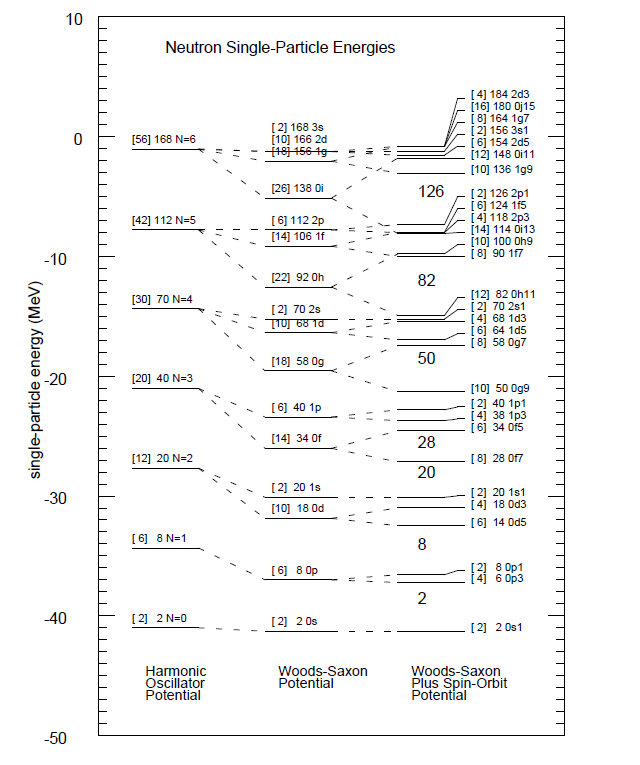
\includegraphics[scale=0.35]{graphics/singleparticle.png}
    \end{figure}
}


\frame
{
  \frametitle{Single-particle Hamiltonians and spin-orbit force}
\begin{small}
{\scriptsize
We have introduced a modified single-particle Hamiltonian
\[
\hat{h}(x_i) =  \hat{t}(x_i) + \hat{u}_{\mathrm{ext}}(x_i) +\xi({\bf r}){\bf ls}=\hat{h}_0(x_i)+\xi({\bf r}){\bf ls}. 
\]
We can calculate the expectation value of the latter using the fact that
\[
\xi({\bf r}){\bf ls}=\frac{1}{2}\xi({\bf r})\left({\bf j}^2-{\bf l}^2-{\bf s}^2\right).
\]
For a single-particle state with quantum numbers $nlj$ (we suppress $s$ and $m_j$), with $s=1/2$ and ${\bf j=l}\pm {\bf s}$, we obtain
the single-particle energies
\[
\varepsilon_{nlj} = \varepsilon_{nlj}^{(0)}+\Delta\varepsilon_{nlj}, 
\]
with $\varepsilon_{nlj}^{(0)}$ being the single-particle energy obtained with $\hat{h}_0(x)$ and 
\[
\Delta\varepsilon_{nlj}=\frac{C}{2}\left(j(j+1)-l(l+1)-\frac{3}{4}\right).
\]
}
\end{small}
}



\frame
{
  \frametitle{Single-particle Hamiltonians and spin-orbit force}
\begin{small}
{\scriptsize
The spin-orbit force gives thus an additional contribution to the energy
\[
\Delta\varepsilon_{nlj}=\frac{C}{2}\left(j(j+1)-l(l+1)-\frac{3}{4}\right),
\]
which lifts the degeneracy we have seen before in the harmonic oscillator or Woods-Saxon potentials. The value $C$ is the radial
integral involving $\xi({\bf r})$. Depending on the value of $j=l\pm 1/2$, we obtain 
\[
\Delta\varepsilon_{nlj=l-1/2}=\frac{C}{2}l,
\]
or
\[
\Delta\varepsilon_{nlj=l+1/2}=-\frac{C}{2}(l+1),
\]
clearly lifting the degeneracy. Note well that till now we have simply postulated the spin-orbit force in {\em ad hoc} way.
Later, we will see how this term arises from the two-nucleon force in a natural way. 
}
\end{small}
}


\frame
{
  \frametitle{Single-particle spin-orbit force and the modified Woods-Saxon potential}
\begin{small}
{\scriptsize
With the spin-orbit force, we can modify our Woods-Saxon potential to 
\[
\hat{u}_{\mathrm{ext}}(r)=-\frac{V_0}{1+\exp{(r-R)/a}}+V_{so}(r){\bf ls},
\]
with 
\[
V_{so}(r) = V_{so}\frac{1}{r}\frac{d f_{so}(r)}{dr},
\]
where we have 
\[
f_{so}(r) = \frac{1}{1+\exp{(r-R_{so})/a_{so}}}.
\]
We can also add, in case of proton, a Coulomb potential. The Woods-Saxon potential has been widely used in parametrizations of
effective single-particle potentials. {\bf However, as was the case with the harmonic oscillator, none of these potentials are linked directly to the nuclear forces}. Our next step is to build a mean field based on the nucleon-nucleon interaction.
This will lead us to our first and simplest many-body theory, Hartree-Fock theory.  

}
\end{small}
}




\frame
{
  \frametitle{Definitions and notations}
\begin{small}
{\scriptsize
Our Hamiltonian is invariant under the permutation (interchange) of two nucleons. % (exercise here, prove it)
Since we deal with fermions, the total wave function is antisymmetric.
Let $\hat{P}$ be an operator which interchanges two nucleons.
Due to the symmetries we have ascribed to our Hamiltonian, this operator commutes with the total Hamiltonian,
\[
[\hat{H},\hat{P}] = 0,
\]
meaning that $\Psi_{\lambda}(x_1, x_2, \dots , x_A)$ is an eigenfunction of 
$\hat{P}$ as well, that is
\[
\hat{P}_{ij}\Psi_{\lambda}(x_1, x_2, \dots,x_i,\dots,x_j,\dots,x_A)=
\beta\Psi_{\lambda}(x_1, x_2, \dots,x_i,\dots,x_j,\dots,x_A),
\]
where $\beta$ is the eigenvalue of $\hat{P}$. We have introduced the suffix $ij$ in order to indicate that we permute nucleons $i$ and $j$.
The Pauli principle tells us that the total wave function for a system of fermions
has to be antisymmetric, resulting in the eigenvalue $\beta = -1$.   
}
\end{small}
}

\frame
{
  \frametitle{Definitions and notations}
\begin{small}
{\scriptsize
In our case we assume that  we can approximate the exact eigenfunction with a Slater determinant
\be
   \Phi(x_1, x_2,\dots ,x_A,\alpha,\beta,\dots, \sigma)=\frac{1}{\sqrt{A!}}
\left| \begin{array}{ccccc} \psi_{\alpha}(x_1)& \psi_{\alpha}(x_2)& \dots & \dots & \psi_{\alpha}(x_A)\\
                            \psi_{\beta}(x_1)&\psi_{\beta}(x_2)& \dots & \dots & \psi_{\beta}(x_A)\\  
                            \dots & \dots & \dots & \dots & \dots \\
                            \dots & \dots & \dots & \dots & \dots \\
                     \psi_{\sigma}(x_1)&\psi_{\sigma}(x_2)& \dots & \dots & \psi_{\sigma}(x_A)\end{array} \right|, 
\label{HartreeFockDet}
\ee 
where  $x_i$  stand for the coordinates and spin values of a nucleon $i$ and $\alpha,\beta,\dots, \gamma$ 
are quantum numbers needed to describe remaining quantum numbers.  
}
\end{small}
}

\frame
{
  \frametitle{Definitions and notations}
\begin{small}
{\scriptsize
The single-nucleon function $\psi_{\alpha}(x_i)$  are eigenfunctions of the one-body
Hamiltonian, that is
\[
\hat{h}_0(x_i)=\hat{t}(x_i) + \hat{u}_{\mathrm{ho}}(x_i),
\]
with eigenvalues 
\[
\hat{h}_0(x_i) \psi_{\alpha}(x_i)=\left(\hat{t}(x_i) + \hat{u}_{\mathrm{ho}}(x_i)\right)\psi_{\alpha}(x_i)=\varepsilon_{\alpha}\psi_{\alpha}(x_i).
\]
The energies $\varepsilon_{\alpha}$ are the so-called non-interacting single-nucleon energies, or unperturbed energies. 
The total energy is in this case the sum over all  single-nucleon energies, if no two-body or more complicated
many-body interactions are present.
}
\end{small}
}


\frame
{
  \frametitle{Definitions and notations}
\begin{small}
{\scriptsize
Let us denote the ground state energy by $E_0$. According to the
variational principle we have
\begin{equation*}
  E_0 \le E[\Phi] = \int \Phi^*\hat{H}\Phi d\mathbf{\tau}
\end{equation*}
where $\Phi$ is a trial function which we assume to be normalized
\begin{equation*}
  \int \Phi^*\Phi d\mathbf{\tau} = 1,
\end{equation*}
where we have used the shorthand $d\mathbf{\tau}=d\mathbf{x}_1d\mathbf{x}_2\dots d\mathbf{x}_A$.
}
\end{small}
}

\frame
{
  \frametitle{Definitions and notations}
\begin{small}
{\scriptsize
In the Hartree-Fock method the trial function is the Slater
determinant of Eq.~(\ref{HartreeFockDet}) which can be rewritten as 
\begin{equation}
  \Phi(x_1,x_2,\dots,x_A,\alpha,\beta,\dots,\nu) = \frac{1}{\sqrt{A!}}\sum_{P} (-)^P\hat{P}\psi_{\alpha}(x_1)
    \psi_{\beta}(x_2)\dots\psi_{\nu}(x_A)=\sqrt{A!}{\cal A}\Phi_H,
\label{HartreeFockPermutation}
\end{equation}
where we have introduced the antisymmetrization operator ${\cal A}$ defined by the 
summation over all possible permutations of two nucleons.
}
\end{small}
}

\frame
{
  \frametitle{Definitions and notations}
\begin{small}
{\scriptsize
It is defined as
\begin{equation}
  {\cal A} = \frac{1}{A!}\sum_{p} (-)^p\hat{P},
\label{antiSymmetryOperator}
\end{equation}
with $p$ standing for the number of permutations. We have introduced for later use the so-called
Hartree-function, defined by the simple product of all possible single-nucleon functions
\begin{equation*}
  \Phi_H(x_1,x_2,\dots,x_A,\alpha,\beta,\dots,\nu) =
  \psi_{\alpha}(x_1)
    \psi_{\beta}(x_2)\dots\psi_{\nu}(x_A).
\end{equation*}

}
\end{small}
}

\frame
{
  \frametitle{Definitions and notations}
\begin{small}
{\scriptsize
Both $\hat{H_0}$ and $\hat{\hat{H}_I}$ are invariant under all possible permutations of any two nucleons
and hence commute with ${\cal A}$
\begin{equation}
  [H_0,{\cal A}] = [H_I,{\cal A}] = 0.
  \label{cummutionAntiSym}
\end{equation}
Furthermore, ${\cal A}$ satisfies
\begin{equation}
  {\cal A}^2 = {\cal A},
  \label{AntiSymSquared}
\end{equation}
since every permutation of the Slater
determinant reproduces it. 
}
\end{small}
}

\frame
{
  \frametitle{Definitions and notations}
\begin{small}
{\scriptsize
The expectation value of $\hat{H_0}$ 
\[
  \int \Phi^*\hat{H_0}\Phi d\mathbf{\tau} 
  = A! \int \Phi_H^*{\cal A}\hat{H_0}{\cal A}\Phi_H d\mathbf{\tau}
\]
is readily reduced to
\[
  \int \Phi^*\hat{H_0}\Phi d\mathbf{\tau} 
  = A! \int \Phi_H^*\hat{H_0}{\cal A}\Phi_H d\mathbf{\tau},
\]
where we have used eqs.~(\ref{cummutionAntiSym}) and
(\ref{AntiSymSquared}). The next step is to replace the antisymmetrization
operator by its definition Eq.~(\ref{HartreeFockPermutation}) and to
replace $\hat{H_0}$ with the sum of one-body operators
\[
  \int \Phi^*\hat{H_0}\Phi  d\mathbf{\tau}
  = \sum_{i=1}^A \sum_{p} (-)^p\int 
  \Phi_H^*\hat{h}_0\hat{P}\Phi_H d\mathbf{\tau}.
\]

}
\end{small}
}

\frame
{
  \frametitle{Definitions and notations}
\begin{small}
{\scriptsize
The integral vanishes if two or more nucleons are permuted in only one
of the Hartree-functions $\Phi_H$ because the individual single-nucleon wave functions are
orthogonal. We obtain then
\[
  \int \Phi^*\hat{H}_0\Phi  d\mathbf{\tau}= \sum_{i=1}^A \int \Phi_H^*\hat{h}_0\Phi_H  d\mathbf{\tau}.
\]
Orthogonality of the single-nucleon functions allows us to further simplify the integral, and we
arrive at the following expression for the expectation values of the
sum of one-body Hamiltonians 
\begin{equation}
  \int \Phi^*\hat{H}_0\Phi  d\mathbf{\tau}
  = \sum_{\mu=1}^A \int \psi_{\mu}^*(\mathbf{x})\hat{h}_0\psi_{\mu}(\mathbf{x})
  d\mathbf{x}.
  \label{H1Expectation}
\end{equation}

}
\end{small}
}

\frame
{
  \frametitle{Definitions and notations}
\begin{small}
{\scriptsize
We introduce the following shorthand for the above integral
\[
\langle \mu | \hat{h}_0 | \mu \rangle = \int \psi_{\mu}^*(\mathbf{x})\hat{h}_0\psi_{\mu}(\mathbf{x})d\mathbf{x}.,
\]
and rewrite Eq.~(\ref{H1Expectation}) as
\begin{equation}
  \int \Phi^*\hat{H_0}\Phi  d\mathbf{\tau}
  = \sum_{\mu=1}^A \langle \mu | \hat{h}_0 | \mu \rangle.
  \label{H1Expectation1}
\end{equation}

}
\end{small}
}
\frame
{
  \frametitle{Definitions and notations}
\begin{small}
{\scriptsize
The expectation value of the two-body part of the Hamiltonian (assuming a two-body Hamiltonian at most) is obtained in a
similar manner. We have
\begin{equation*}
  \int \Phi^*\hat{H_I}\Phi d\mathbf{\tau} 
  = A! \int \Phi_H^*{\cal A}\hat{H_I}{\cal A}\Phi_H d\mathbf{\tau},
\end{equation*}
which reduces to
\begin{equation*}
 \int \Phi^*\hat{H_I}\Phi d\mathbf{\tau} 
  = \sum_{i\le j=1}^A \sum_{p} (-)^p\int 
  \Phi_H^*\hat{v}(x_{ij})\hat{P}\Phi_H d\mathbf{\tau},
\end{equation*}
by following the same arguments as for the one-body
Hamiltonian. 
}
\end{small}
}
\frame
{
  \frametitle{Definitions and notations}
\begin{small}
{\scriptsize
Because of the dependence on the inter-nucleon distance $r_{ij}$,  permutations of
any two nucleons no longer vanish, and we get
\begin{equation*}
  \int \Phi^*\hat{H_I}\Phi d\mathbf{\tau} 
  = \sum_{i < j=1}^A \int  
  \Phi_H^*\hat{v}(x_{ij})(1-P_{ij})\Phi_H d\mathbf{\tau}.
\end{equation*}
where $P_{ij}$ is the permutation operator that interchanges
nucleon $i$ and nucleon $j$. Again we use the assumption that the single-nucleon wave functions
are orthogonal. 
}
\end{small}
}
\frame
{
  \frametitle{Definitions and notations}
\begin{small}
{\scriptsize
We obtain
\begin{equation}
\begin{split}
  \int \Phi^*\hat{H_I}\Phi d\mathbf{\tau} 
  = \frac{1}{2}\sum_{\mu=1}^A\sum_{\nu=1}^A
    &\left[ \int \psi_{\mu}^*(x_i)\psi_{\nu}^*(x_j)\hat{v}(x_{ij})\psi_{\mu}(x_i)\psi_{\nu}(x_j)
    dx_idx_j \right.\\
  &\left.
  - \int \psi_{\mu}^*(x_i)\psi_{\nu}^*(x_j)
  \hat{v}(x_{ij})\psi_{\nu}(x_i)\psi_{\mu}(x_j)
  dx_idx_j
  \right]. \label{H2Expectation}
\end{split}
\end{equation}
The first term is the so-called direct term. In Hartree-Fock theory it leads to the so-called Hartree term, 
while the second is due to the Pauli principle and is called
the exchange term and in Hartree-Fock theory it defines the so-called xFock term.
The factor  $1/2$ is introduced because we now run over
all pairs twice. 
}
\end{small}
}
\frame
{
  \frametitle{Definitions and notations}
\begin{small}
{\scriptsize
The last equation allows us to  introduce some further definitions.  
The single-nucleon wave functions $\psi_{\mu}({\bf x})$, defined by the quantum numbers $\mu$ and ${\bf x}$
(recall that ${\bf x}$ also includes spin degree, later we will also add isospin)   are defined as the overlap 
\[
   \psi_{\alpha}(x)  = \langle x | \alpha \rangle .
\]

}
\end{small}
}
\frame
{
  \frametitle{Definitions and notations}
\begin{small}
{\scriptsize
We introduce the following shorthands for the above two integrals
\[
\langle \mu\nu|V|\mu\nu\rangle =  \int \psi_{\mu}^*(x_i)\psi_{\nu}^*(x_j)\hat{v}(x_{ij})\psi_{\mu}(x_i)\psi_{\nu}(x_j)
    dx_idx_j,
\]
and 
\[
\langle \mu\nu|V|\nu\mu\rangle = \int \psi_{\mu}^*(x_i)\psi_{\nu}^*(x_j)
  \hat{v}(x_{ij})\psi_{\nu}(x_i)\psi_{\mu}(x_j)
  dx_idx_j.  
\]
}
\end{small}
}
\frame
{
  \frametitle{Definitions and notations}
\begin{small}
{\scriptsize
The direct and exchange matrix elements can be  brought together if we define the antisymmetrized matrix element
\[
\langle \mu\nu|V|\mu\nu\rangle_{\mathrm{AS}}= \langle \mu\nu|V|\mu\nu\rangle-\langle \mu\nu|V|\nu\mu\rangle,
\]
or for a general matrix element  
\[
\langle \mu\nu|V|\sigma\tau\rangle_{\mathrm{AS}}= \langle \mu\nu|V|\sigma\tau\rangle-\langle \mu\nu|V|\tau\sigma\rangle.
\]
It has the symmetry property
\[
\langle \mu\nu|V|\sigma\tau\rangle_{\mathrm{AS}}= -\langle \mu\nu|V|\tau\sigma\rangle_{\mathrm{AS}}=-\langle \nu\mu|V|\sigma\tau\rangle_{\mathrm{AS}}.
\]
}
\end{small}
}
\frame
{
  \frametitle{Definitions and notations}
\begin{small}
{\scriptsize
The antisymmetric matrix element is also hermitian, implying 
\[
\langle \mu\nu|V|\sigma\tau\rangle_{\mathrm{AS}}= \langle \sigma\tau|V|\mu\nu\rangle_{\mathrm{AS}}.
\]

With these notations we rewrite Eq.~(\ref{H2Expectation}) as 
\begin{equation}
  \int \Phi^*\hat{H_I}\Phi d\mathbf{\tau} 
  = \frac{1}{2}\sum_{\mu=1}^A\sum_{\nu=1}^A \langle \mu\nu|V|\mu\nu\rangle_{\mathrm{AS}}.
\label{H2Expectation2}
\end{equation}

}
\end{small}
}
\frame
{
  \frametitle{Definitions and notations}
\begin{small}
{\scriptsize
Combining Eqs.~(\ref{H1Expectation1}) and
(\ref{H2Expectation2}) we obtain the energy functional 
\begin{equation}
  E[\Phi] 
  = \sum_{\mu=1}^A \langle \mu | \hat{h}_0 | \mu \rangle +
  \frac{1}{2}\sum_{{\mu}=1}^A\sum_{{\nu}=1}^A \langle \mu\nu|V|\mu\nu\rangle_{\mathrm{AS}}.
\label{FunctionalEPhi}
\end{equation}
which we will use as our starting point for the Hartree-Fock calculations later in this course. 
}
\end{small}
}



\frame[containsverbatim]
{
  \frametitle{Hartree-Fock: our first many-body approach}
\begin{small}
{\scriptsize
HF theory is an algorithm for a finding an approximative expression for the ground state of a given
Hamiltonian. The basic ingredients are
\begin{itemize}
\item Define a single-particle basis $\{\psi_{\alpha}\}$ so that
\[ \hat{h}^{\mathrm{HF}}\psi_{\alpha} = \varepsilon_{\alpha}\psi_{\alpha}\]
with 
\[
\hat{h}^{\mathrm{HF}}=\hat{t}+\hat{u}_{\mathrm{ext}}+\hat{u}^{\mathrm{HF}}
\]
\item where $\hat{u}^{\mathrm{HF}}$ is a single-particle potential to be determined by the HF algorithm.
\item The HF algorithm means to choose $\hat{u}^{\mathrm{HF}}$ in order to have 
\[ \langle \hat{H} \rangle = E^{\mathrm{HF}}= \langle \Phi_0 | \hat{H}|\Phi_0 \rangle\]
a local minimum with $\Phi_0$ being the SD ansatz for the ground state. 
\item The variational principle ensures that $E^{\mathrm{HF}} \ge \tilde{E}_0$, $\tilde{E}_0$ the exact ground state energy.
\end{itemize}

 }
 \end{small}
 }


\frame[containsverbatim]
{
  \frametitle{Hartree-Fock: }
\begin{small}
{\scriptsize
Let us now compute the  Hamiltonian matrix for a system consisting of a Slater determinant for the ground state 
$|\Phi_0 \rangle$ and two 1p1h SDs $|\Phi_i^a \rangle$ and $|\Phi_j^b \rangle$. This can obviously be generalized to many more 1p1h SDs.  We will show later that  we get the following 
expectation values
\[ \langle \Phi_0 | \hat{H}|\Phi_0 \rangle = E_0, \]
\[ \langle \Phi_i^a | \hat{H}|\Phi_0 \rangle = \langle a | \hat{f} | i \rangle,\]
\[ \langle \Phi_j^b | \hat{H}|\Phi_0 \rangle = \langle b | \hat{f} | j \rangle,\]
\[\langle \Phi_i^a | \hat{H}|\Phi_j^b \rangle = \langle aj | \hat{v} | ib \rangle,\]
and the diagonal elements
\[ \langle \Phi_i^a | \hat{H}|\Phi_i^a \rangle = E_0+\varepsilon_{a}-\varepsilon_{i}+\langle ai | \hat{v} | ia \rangle,\]
and 
\[ \langle \Phi_j^b | \hat{H}|\Phi_j^b \rangle =E_0+\varepsilon_{b}-\varepsilon_{j}+\langle bj | \hat{v} | jb \rangle.\]
{\bf NOTE:} These equations and those on the next slide will be derived during week 5 (end of january).
 }
 \end{small}
 }



\frame[containsverbatim]
{
  \frametitle{Hartree-Fock}
\begin{small}
{\scriptsize
We can then set up a Hamiltonian matrix to be diagonalized
\[
 \left( \begin{array}{ccc} 
               E_0  & \langle i | \hat{f} | a \rangle &  \langle j | \hat{f} | b\rangle\\
               \langle a | \hat{f} | i \rangle  &E_0+\varepsilon_{a}-\varepsilon_{i}+\langle ai | \hat{v} | ia \rangle  & \langle aj | \hat{v} | ib \rangle      \\
               \langle b | \hat{f} | j \rangle  & \langle bi | \hat{v} | ja \rangle &E_0+\varepsilon_{b}-\varepsilon_{j}+\langle bj | \hat{v} | jb \rangle         \\
             \end{array} \right) .
\]
The HF method corresponds to finding a similarity transformation where the non-diagonal matrix elements
\[\langle i | \hat{f} | a \rangle=0\].   We will link this expectation value with the HF method, meaning that
we want to find
\[\langle i | \hat{h}^{\mathrm{HF}}| a \rangle=0\]
 }
 \end{small}
 }


\frame
{
  \frametitle{How to solve Schr\"odinger's equation for single-particle potentials}
\begin{small}
{\scriptsize
Before we proceed, we need to discuss the single-particle states which enter the definition of the Slater determinant. We will start with hydrogen-like orbits, which is a case you probably have seen before. It is then easy to switch to 
a harmonic oscillator or Woods-Saxon basis.
To achieve this, we need to refresh our knowledge about the Schr\"odinger equation for the hydrogen atom.

To solve the Schr\"odinger equation as a matrix diagonalization problem,
let us study the radial part of the Schr\"odinger equation. 
The radial part of the wave function, $R(r)$, is a solution to  
%
\[
  -\frac{\hbar^2}{2 m} \left ( \frac{1}{r^2} \frac{d}{dr} r^2
  \frac{d}{dr} - \frac{l (l + 1)}{r^2} \right )R(r) 
     + V(r) R(r) = E R(r).
\]
Here we use $V(r) = -Z/r$.
}
\end{small}
}

\frame
{
  \frametitle{How to solve Schr\"odinger's equation for single-particle potentials}
\begin{small}
{\scriptsize
%
Then we substitute $R(r) = (1/r) u(r)$ and obtain
%
\[
  -\frac{\hbar^2}{2 m} \frac{d^2}{dr^2} u(r) 
       + \left ( V(r) + \frac{l (l + 1)}{r^2}\frac{\hbar^2}{2 m}
                                    \right ) u(r)  = E u(r) .
\]
%
We introduce a dimensionless variable $\rho = (1/\alpha) r$
where $\alpha$ is a constant with dimension length and get
% 
\[
  -\frac{\hbar^2}{2 m \alpha^2} \frac{d^2}{d\rho^2} u(\rho) 
       + \left ( V(\rho) + \frac{l (l + 1)}{\rho^2}
         \frac{\hbar^2}{2 m\alpha^2} \right ) u(\rho)  = E u(\rho) .
\]
}
\end{small}
}


\frame
{
  \frametitle{How to solve Schr\"odinger's equation for single-particle potentials}
\begin{small}
{\scriptsize
%
We replace $\rho$ with $x$, take away the 
centrifugal barrier (that is setting $l=0$) term and set the potential equal to
\[
   V(x)=-\frac{kZ}{x\alpha},
\]
with  $k=1.44$ eVnm being a constant. We multiply with $m \alpha^2/\hbar^2$ and since $\alpha$ is just a constant, we fix it by requiring that
\[
\frac{kZm \alpha}{\hbar^2}=1,
\]
giving 
\[
\alpha = \frac{\hbar^2}{kZm},
\]
which is the Bohr radius and leads to a natural length scale.
This leads to the equation
\[
  -\frac{1}{2} \frac{d^2}{dx^2} u(x) -\frac{1}{x}u(x)  = \lambda u(x),
\]
with 
\[
\lambda = \frac{E m \alpha^2}{\hbar^2}. 
\]
}
\end{small}
}


%



\frame
{
  \frametitle{How to solve Schr\"odinger's equation for single-particle potentials}
\begin{small}
{\scriptsize
Let us now see how we can rewrite this equation as a matrix eigenvalue problem.
First we need to compute  the second derivative. We use here the
following expression for the second derivative of a function $f$
\[
    f''=\frac{f(x+h) -2f(x) +f(x-h)}{h^2} +O(h^2),
\]
where $h$ is our step.
Next we define minimum and maximum values for the variable $x$,
$R_{\mathrm{min}}$  and $R_{\mathrm{max}}$, respectively.
With a given number of steps, $N_{\mathrm{step}}$, we then 
define the step $h$ as
\[
  h=\frac{R_{\mathrm{max}}-R_{\mathrm{min}} }{N_{\mathrm{step}}}.
\]

}
\end{small}
}


\frame
{
  \frametitle{How to solve Schr\"odinger's equation for single-particle potentials}
\begin{small}
{\scriptsize
We discretize  $x$ as 
\[
    x_i= R_{\mathrm{min}} + ih \hspace{1cm} i=1,2,\dots , N_{\mathrm{step}}-1
\]
we can rewrite the Schr\"odinger equation for $x_i$ as
\[
-\frac{1}{2}\frac{u(x_k+h) -2u(x_k) +u(x_k-h)}{h^2}-\frac{1}{x_k}u(x_k)  = \lambda u(x_k),
\]
or in  a more compact way
\[
-\frac{1}{2}\frac{u_{k+1} -2u_k +u_{k-1}}{h^2}-\frac{1}{x_k}u_k=-\frac{1}{2}\frac{u_{k+1} -2u_k +u_{k-1} }{h^2}+V_ku_k  = \lambda u_k,
\]
where $u_k=u(x_k)$, $u_{k\pm 1}=u(x_k\pm h)$ and $V_k=-1/x_k$, the given potential.
}
\end{small}
}


\frame
{
  \frametitle{How to solve Schr\"odinger's equation for single-particle potentials}
\begin{small}
{\scriptsize
Let us see how this recipe may lead to a matrix reformulation of the 
Schr\"odinger equation.
Define first the diagonal matrix element
\[
   d_k=\frac{1}{h^2}+V_k,
\]
and the non-diagonal matrix element 
\[
   e_k=-\frac{1}{2h^2}.
\]
In this case the non-diagonal matrix elements are given by a mere constant.
{\em All non-diagonal matrix elements are equal}.
With these definitions the Schr\"odinger equation takes the following form
\[
d_ku_k+e_{k-1}u_{k-1}+e_{k+1}u_{k+1}  = \lambda u_k,
\]
where $u_k$ is unknown.
}
\end{small}
}


\frame
{
  \frametitle{How to solve Schr\"odinger's equation for single-particle potentials}
\begin{small}
{\scriptsize
 Since we have $N_{\mathrm{step}}$ values of $k$ we can write the 
latter equation as a matrix eigenvalue problem 
\begin{equation}
    \left( \begin{array}{ccccccc} d_1 & e_1 & 0   & 0    & \dots  &0     & 0 \\
                                e_1 & d_2 & e_2 & 0    & \dots  &0     &0 \\
                                0   & e_2 & d_3 & e_3  &0       &\dots & 0\\
                                \dots  & \dots & \dots & \dots  &\dots      &\dots & \dots\\
                                0   & \dots & \dots & \dots  &\dots       &d_{N_{\mathrm{step}}-1} & e_{N_{\mathrm{step}}-1}\\
                                0   & \dots & \dots & \dots  &\dots       &e_{N_{\mathrm{step}}-1} & d_{N_{\mathrm{step}}}

             \end{array} \right)      \left( \begin{array}{c} u_{1} \\
                                                              u_{2} \\
                                                              \dots\\ \dots\\ \dots\\
                                                              u_{N_{\mathrm{step}}}
             \end{array} \right)=\lambda \left( \begin{array}{c} u_{1} \\
                                                              u_{2} \\
                                                              \dots\\ \dots\\ \dots\\
                                                              u_{N_{\mathrm{step}}}
             \end{array} \right) 
      \label{eq:sematrix}
\end{equation} 
When setting up the matrix, be careful with the endpoints. Our wave function has the values $u(0) =u(\infty)=0$ and you don't need to include these points in the equations.
}
\end{small}
}



\frame
{
  \frametitle{How to solve Schr\"odinger's equation for single-particle potentials}
\begin{small}
{\scriptsize
This is a matrix problem with a tridiagonal matrix of dimension 
$N_{\mathrm{step}} \times N_{\mathrm{step}}$ and will thus yield 
$N_{\mathrm{step}}$ eigenvalues. 

The algorithm for solving this problem  may take the following 
form 
\begin{itemize}
  \item Define values for $N_{\mathrm{step}}$, $R_{\mathrm{min}}$ and $R_{\mathrm{max}}$.
        These values define in turn the step size $h$. Typical values for
        $R_{\mathrm{max}}$ and $R_{\mathrm{min}}$ could be $0$ and $10$ respectively for the lowest-lying states.  
        The number of mesh points $N_{\mathrm{step}}$ could be in the range 100 to some
        thousands. You can check the stability of the results as functions of 
        $N_{\mathrm{step}}$ and $R_{\mathrm{max}}$ and $R_{\mathrm{min}}$
        against the exact solutions. 
  \item Construct then two one-dimensional arrays which contain all values of $x_k$ 
        and the potential $V_k$. For the latter it can be convenient to write a
        small function which sets up the potential as function of $x_k$. For 
        the three-dimensional case you may also need to include 
        the centrifugal potential. 
\end{itemize} 


}
\end{small}
}
\frame
{
  \frametitle{How to solve Schr\"odinger's equation for single-particle potentials}
\begin{small}
{\scriptsize
\begin{itemize}
  \item Construct thereafter the one-dimensional vectors $d$ and $e$, where 
        $d$ stands for the diagonal matrix elements and $e$ the non-diagonal ones.
        Be careful with the endpoints, since we know the wave function $u$ at both ends of the
        chosen grid.   
  \item We are now ready to obtain the eigenvalues by calling the function {\em tqli }, see the code examples
        at the webpage.
        Calling {\em tqli}, you have to transfer the 
        vectors  $d$ and $e$ and their dimension
        dimension $n=N_{\mathrm{step}}$ and a matrix $z$ of dimension
        $N_{\mathrm{step}}1\times N_{\mathrm{step}}$ which returns the eigenfunctions.
        On return, the array $d$ contains the 
        eigenvalues. If $z$ is given as the unity matrix on input, it returns the 
       eigenvectors. For a given eigenvalue $k$, the eigenvector is given by the column
       $k$ in $z$, that is z[][k] in C, or z(:,k) in Fortran. Alternatively, if you use armadillo, see below, you would call one of the armadillo functions or lapack functions.
\end{itemize} 

}
\end{small}
}




\frame[containsverbatim]
{
  \frametitle{Example of c++ code for solving Schr\"odinger's equation and read and write to file}
\begin{small}
{\scriptsize
We are using armadillo here. For standard c++, see the code example on the webpage. Idem for the Fortran code.
\begin{lstlisting}
/*
  Solves the one-particle Schrodinger equation
  for a potential specified in function
  potential(). This example is for the harmonic oscillator
  compile as c++ -O3 -o ho3d.x ho3d.cpp -larmadillo -llapack -lblas
*/
#include <cmath>
#include <iostream>
#include <fstream>
#include <iomanip>
#include <armadillo>
using namespace  std;
using namespace arma;
// output file as global variable
ofstream ofile;  
\end{lstlisting}
}
\end{small}
}


\frame[containsverbatim]
{
  \frametitle{Example of c++ code for solving Schr\"odinger's equation and read and write to file}
\begin{small}
{\scriptsize
\begin{lstlisting}
// function declarations 
double Potential(double);
// Main program starts here
int main(int argc, char* argv[])
{
  int       i, j, MaxStep, OrbL;
  double    Rmax, Step, Const1, Const2, OrbitalFactor ;
  char *outfilename;
\end{lstlisting}
}
\end{small}
}


\frame[containsverbatim]
{
  \frametitle{Example of c++ code for solving Schr\"odinger's equation and read and write to file}
\begin{small}
{\scriptsize
\begin{lstlisting}
  // Read in output file, abort if there are too few command-line arguments
  if( argc <= 4 ){
    cout << "Bad Usage: " << argv[0] << 
      " read also output file on same line, Rmax, Orbital momentum and Max steps" << endl;
    exit(1);
  }
  else{
    outfilename=argv[1];
    Rmax = atof(argv[2]);
    OrbL = atoi(argv[3]);
    MaxStep = atoi(argv[4]);
  }
  ofile.open(outfilename); 
\end{lstlisting}
}
\end{small}
}


\frame[containsverbatim]
{
  \frametitle{Example of c++ code for solving Schr\"odinger's equation and read and write to file}
\begin{small}
{\scriptsize
\begin{lstlisting}
  // initialise constants assuming Rmin = 0.0;
  Step    = Rmax / (MaxStep+1); 
  Const2 = -0.5 / (Step * Step);   Const1 = 1.0 / (Step * Step);
  OrbitalFactor = OrbL * (OrbL + 1);
  //  set up r, diagonal and non-diagonal elements 
  vec r(MaxStep+1), d(MaxStep-1), e(MaxStep-1);
  for(i = 0; i < MaxStep-1; i++) {
    r(i) = (i+1) * Step;   // avoid r = 0 and infty, known values
    d(i) = Const1+ Potential(r(i)) + 0.5*OrbitalFactor / (r(i) * r(i));
  }
\end{lstlisting}
}
\end{small}
}


\frame[containsverbatim]
{
  \frametitle{Example of c++ code for solving Schr\"odinger's equation and read and write to file}
\begin{small}
{\scriptsize
\begin{lstlisting}
  e = Const2;
  mat A(MaxStep-1,MaxStep-1);
  // Set up matrix
  for(i = 0; i < MaxStep-1; i++) {
    // Diagonal elements
    A(i,i) = d(i);
    // Non-diagonal elements
    if (i < MaxStep - 2) {
      A(i,i + 1) = Const2;
      A(i + 1,i) = Const2;
    }
  }
\end{lstlisting}
}
\end{small}
}


\frame[containsverbatim]
{
  \frametitle{Example of c++ code for solving Schr\"odinger's equation and read and write to file}
\begin{small}
{\scriptsize
\begin{lstlisting}
  vec eigval(MaxStep-1);
  mat eigvec(MaxStep-1,MaxStep-1);
  //  The eigenvectors are normalized
  eig_sym(eigval, eigvec, A);
\end{lstlisting}
}
\end{small}
}


\frame[containsverbatim]
{
  \frametitle{Example of c++ code for solving Schr\"odinger's equation and read and write to file}
\begin{small}
{\scriptsize
\begin{lstlisting}
  // print results
  ofile << "RESULTS:" << endl;
  ofile << setiosflags(ios::showpoint | ios::uppercase);
  ofile <<"R_max = " << setw(15) << setprecision(8) << Rmax << endl;  
  ofile <<"Number of steps = " << setw(15) << MaxStep << endl;  
  ofile << "Lowest eigenvalue:" << endl;
  ofile << setw(15) << setprecision(8) << eigval(0) << endl;
  for(i = 0; i < MaxStep-1; i++) {
    ofile << setw(15) << setprecision(8) << r(i);
    //    ofile << setw(15) << setprecision(8) << 2*exp(-r(i)*r(i)*0.5)/pow(acos(-1.0),0.25);
    ofile << setw(15) << setprecision(8) << eigvec(i,0)*eigvec(i,0) << endl;
  }
  ofile.close();  // close 
  return 0;
} // End: function main() 
\end{lstlisting}
}
\end{small}
}


\frame[containsverbatim]
{
  \frametitle{Example of c++ code for solving Schr\"odinger's equation and read and write to file}
\begin{small}
{\scriptsize
\begin{lstlisting}
/*
  The function potential()
  calculates and return the value of the 
  potential for a given argument x.
  The potential here is the harmonic oscillator
*/        
double Potential(double x)
{
  return 0.5*x*x;

} // End: function potential()  
\end{lstlisting}
}
\end{small}
}







\section[Week 4]{Week 4}

\frame
{
  \frametitle{Topics for Week 4, January 20-24}
  \begin{block}{Hartree-Fock theory and second-quantization}
\begin{itemize}
\item Wednesday:
\item Repetition from last week
\item Derivation of the Hartree-Fock equations by varying the single-particle functions or the coefficients of the 
single-particle equations.
\item Friday:
\item More discussion of Hartree-Fock and perhaps (if time) introduction of creation and annihilation operators
\item Discussion of exercises 3, 4 and optional exercise 4 which is numerical.
\end{itemize}
Suggested literature is AB chapter 14 and JS chapter 4. 
  \end{block}
} 




\frame[containsverbatim]
{
  \frametitle{Background material: Variational Calculus and Lagrangian Multiplier}
\begin{small}
{\scriptsize
The calculus of variations involves 
problems where the quantity to be minimized or maximized is an integral. 

In the general case we have an integral of the type
\[ E[\Phi]= \int_a^b f(\Phi(x),\frac{\partial \Phi}{\partial x},x)dx,\]
where $E$ is the quantity which is sought minimized or maximized.
The problem is that although $f$ is a function of the variables $\Phi$, $\partial \Phi/\partial x$ and $x$, the exact dependence of
$\Phi$ on $x$ is not known.  This means again that even though the integral has fixed limits $a$ and $b$, the path of integration is
not known. In our case the unknown quantities are the single-particle wave functions and we wish to choose an integration path which makes
the functional $E[\Phi]$ stationary. This means that we want to find minima, or maxima or saddle points. In physics we search normally for minima.
Our task is therefore to find the minimum of $E[\Phi]$ so that its variation $\delta E$ is zero  subject to specific
constraints. In our case the constraints appear as the integral which expresses the orthogonality of the  single-particle wave functions.
The constraints can be treated via the technique of Lagrangian multipliers
 }
 \end{small}
 }


\frame[containsverbatim]
{
  \frametitle{Background material: Euler-Lagrange equations}
\begin{small}
{\scriptsize
We assume the existence of an optimum path, that is a path for which $E[\Phi]$ is stationary. There are infinitely many such paths.
The difference between two paths $\delta\Phi$ is called the variation of $\Phi$.

We call the variation $\eta(x)$  and it is scaled by a factor $\alpha$.  The function $\eta(x)$ is arbitrary except
for 
\[ 
\eta(a)=\eta(b)=0,
\]
and we assume that we can model the change in $\Phi$ as 
\[
\Phi(x,\alpha) = \Phi(x,0)+\alpha\eta(x),
\]
and 
\[
\delta\Phi = \Phi(x,\alpha) -\Phi(x,0)=\alpha\eta(x).
\]
 }
 \end{small}
 }


\frame[containsverbatim]
{
  \frametitle{Background material: Euler-Lagrange equations}
\begin{small}
{\scriptsize
We choose $\Phi(x,\alpha=0)$ as the unkonwn path  that will minimize $E$.  The value 
$\Phi(x,\alpha\ne 0)$  describes a neighbouring path. 
 
We have
\[ E[\Phi(\alpha)]= \int_a^b f(\Phi(x,\alpha),\frac{\partial \Phi(x,\alpha)}{\partial x},x)dx.\] 
In the slides I will use  the shorthand
\[
\Phi_x(x,\alpha) = \frac{\partial \Phi(x,\alpha)}{\partial x}.
\]
In our case $a=0$ and $b=\infty$ and we know the value of the wave function.
 }
 \end{small}
 }




\frame[containsverbatim]
{
  \frametitle{Background material: Euler-Lagrange equations}
\begin{small}
{\scriptsize
The condition for an extreme of
\[ E[\Phi(\alpha)]= \int_a^b f(\Phi(x,\alpha),\Phi_x(x,\alpha),x)dx,\]
is
\[
\left[\frac{\partial  E[\Phi(\alpha)]}{\partial x}\right]_{\alpha=0} =0.\]
The $\alpha$ dependence is contained in $\Phi(x,\alpha)$ and $\Phi_x(x,\alpha)$ meaning that
\[
\left[\frac{\partial  E[\Phi(\alpha)]}{\partial \alpha}\right]=\int_a^b \left( \frac{\partial f}{\partial \Phi}\frac{\partial \Phi}{\partial \alpha}+\frac{\partial f}{\partial \Phi_x}\frac{\partial \Phi_x}{\partial \alpha}        \right)dx.\]
We have defined 
\[
\frac{\partial \Phi(x,\alpha)}{\partial \alpha}=\eta(x)
\]
and thereby 
\[
\frac{\partial \Phi_x(x,\alpha)}{\partial \alpha}=\frac{d(\eta(x))}{dx}.
\]

 }
 \end{small}
 }



\frame[containsverbatim]
{
  \frametitle{Background material: Euler-Lagrange equations}
\begin{small}
{\scriptsize
Using
\[
\frac{\partial \Phi(x,\alpha)}{\partial \alpha}=\eta(x),
\]
and 
\[
\frac{\partial \Phi_x(x,\alpha)}{\partial \alpha}=\frac{d(\eta(x))}{dx},
\]
in the integral gives 
\[
\left[\frac{\partial  E[\Phi(\alpha)]}{\partial \alpha}\right]=\int_a^b \left( \frac{\partial f}{\partial \Phi}\eta(x)+\frac{\partial f}{\partial \Phi_x}\frac{d(\eta(x))}{dx}        \right)dx.\]
Integrate the second term by parts

\[
\int_a^b \frac{\partial f}{\partial \Phi_x}\frac{d(\eta(x))}{dx}dx =\eta(x)\frac{\partial f}{\partial \Phi_x}|_a^b-
\int_a^b \eta(x)\frac{d}{dx}\frac{\partial f}{\partial \Phi_x}dx, 
\]
and since the first term dissappears due to $\eta(a)=\eta(b)=0$, we obtain
\[
\left[\frac{\partial  E[\Phi(\alpha)]}{\partial \alpha}\right]=\int_a^b \left( \frac{\partial f}{\partial \Phi}-\frac{d}{dx}\frac{\partial f}{\partial \Phi_x}
\right)\eta(x)dx=0.\]

 }
 \end{small}
 }


\frame[containsverbatim]
{
  \frametitle{Background material: Euler-Lagrange equations}
\begin{small}
{\scriptsize
\[
\left[\frac{\partial  E[\Phi(\alpha)]}{\partial \alpha}\right]=\int_a^b \left( \frac{\partial f}{\partial \Phi}-\frac{d}{dx}\frac{\partial f}{\partial \Phi_x}
\right)\eta(x)dx=0,\]
can also be written as 
\[
\alpha\left[\frac{\partial  E[\Phi(\alpha)]}{\partial \alpha}\right]_{\alpha=0}=\int_a^b \left( \frac{\partial f}{\partial \Phi}-\frac{d}{dx}\frac{\partial f}{\partial \Phi_x}
\right)\delta\Phi(x)dx=\delta E = 0.\]

The condition for a stationary value is thus a partial differential equation
\[
\frac{\partial f}{\partial \Phi}-\frac{d}{dx}\frac{\partial f}{\partial \Phi_x}=0,\]
known as Euler's equation.
Can easily be generalized to more variables.
 }
 \end{small}
 }


\frame[containsverbatim]
{
  \frametitle{Background material: Lagrangian Multipliers}
\begin{small}
{\scriptsize
Consider a function of three independent variables $f(x,y,z)$ . For the function $f$ to be an 
extreme we have
\[
df=0.
\]
A necessary and sufficient condition is
\[
\frac{\partial f}{\partial x} =\frac{\partial f}{\partial y}=\frac{\partial f}{\partial z}=0,
\]
due to 
\[
df = \frac{\partial f}{\partial x}dx+\frac{\partial f}{\partial y}dy+\frac{\partial f}{\partial z}dz.
\]
In physical problems the variables $x,y,z$ are often subject to constraints (in our case $\Phi$ and the orthogonality constraint)
so that they are no longer all independent. It is possible at least in principle to use each constraint to eliminate one variable
and to proceed with a new and smaller set of independent varables.
 }
 \end{small}
 }



\frame[containsverbatim]
{
  \frametitle{Background material: Lagrangian Multipliers}
\begin{small}
{\scriptsize
The use of so-called Lagrangian  multipliers is an alternative technique  when the elimination of
of variables is incovenient or undesirable.  Assume that we have an equation of constraint on the variables $x,y,z$
\[
\phi(x,y,z) = 0,
\]
 resulting in
\[
d\phi = \frac{\partial \phi}{\partial x}dx+\frac{\partial \phi}{\partial y}dy+\frac{\partial \phi}{\partial z}dz =0.
\]
Now we cannot set anymore 
\[
\frac{\partial f}{\partial x} =\frac{\partial f}{\partial y}=\frac{\partial f}{\partial z}=0,
\]
if $df=0$ is wanted 
because there are now only two independent variables!  Assume $x$ and $y$ are the independent variables.
Then $dz$ is no longer arbitrary. 
 }
 \end{small}
 }



\frame[containsverbatim]
{
  \frametitle{Background material: Lagrangian Multipliers}
\begin{small}
{\scriptsize
However, we can add to
\[
df = \frac{\partial f}{\partial x}dx+\frac{\partial f}{\partial y}dy+\frac{\partial f}{\partial z}dz,
\]
a multiplum of $d\phi$, viz. $\lambda d\phi$, resulting  in

\[
df+\lambda d\phi = (\frac{\partial f}{\partial z}+\lambda\frac{\partial \phi}{\partial x})dx+(\frac{\partial f}{\partial y}+\lambda\frac{\partial \phi}{\partial y})dy+
(\frac{\partial f}{\partial z}+\lambda\frac{\partial \phi}{\partial z})dz =0.
\]
Our multiplier is chosen so that
\[
\frac{\partial f}{\partial z}+\lambda\frac{\partial \phi}{\partial z} =0.
\]
 }
 \end{small}
 }



\frame[containsverbatim]
{
  \frametitle{Background material: Lagrangian Multipliers}
\begin{small}
{\scriptsize
However, we took $dx$ and $dy$ as to be arbitrary and thus we must have
\[
\frac{\partial f}{\partial x}+\lambda\frac{\partial \phi}{\partial x} =0,
\]
and
\[
\frac{\partial f}{\partial y}+\lambda\frac{\partial \phi}{\partial y} =0.
\]
When all these equations are satisfied, $df=0$.  We have four unknowns, $x,y,z$ and
$\lambda$. Actually we want only $x,y,z$, $\lambda$ need not to be determined, it is therefore often called
Lagrange's undetermined multiplier. 
If we have a set of constraints $\phi_k$ we have the equations
\[
\frac{\partial f}{\partial x_i}+\sum_k\lambda_k\frac{\partial \phi_k}{\partial x_i} =0.
\]
 }
 \end{small}
 }








\frame[containsverbatim]
{
  \frametitle{Background material: Variational Calculus and Lagrangian Multipliers}
\begin{small}
{\scriptsize
Let us specialize to the expectation value of the energy for one particle in three-dimensions.
This expectation value reads
\[
  E=\int dxdydz \psi^*(x,y,z) \hat{H} \psi(x,y,z),
\]
with the constraint
\[
 \int dxdydz \psi^*(x,y,z) \psi(x,y,z)=1,
\]
and a Hamiltonian
\[
\hat{H}=-\frac{1}{2}\nabla^2+\hat{v}(x,y,z).
\]
I will skip the variables $x,y,z$ below, and write for example $\hat{v}(x,y,z)=V$.
 }
 \end{small}
 }


\frame[containsverbatim]
{
  \frametitle{Background material: Variational Calculus and Lagrangian Multiplier}
\begin{small}
{\scriptsize
The integral involving the kinetic energy can be written as, if we assume periodic boundary conditions or that the function $\psi$ vanishes
strongly for large values of $x,y,z$, 
 \[
  \int dxdydz \psi^* \left(-\frac{1}{2}\nabla^2\right) \psi dxdydz = -\psi^*\nabla\psi|+\int dxdydz\frac{1}{2}\nabla\psi^*\nabla\psi.
\]
Inserting this expression into the expectation value for the energy and taking the variational minimum  we obtain
\[
\delta E = \delta \left\{\int dxdydz\left( \frac{1}{2}\nabla\psi^*\nabla\psi+V\psi^*\psi\right)\right\} = 0.
\]
 }
 \end{small}
 }

\frame[containsverbatim]
{
  \frametitle{Background material: Variational Calculus and Lagrangian Multiplier}
\begin{small}
{\scriptsize
The constraint appears in integral form as 
\[
 \int dxdydz \psi^* \psi=\mathrm{constant},
\]
and multiplying with a Lagrangian multiplier $\lambda$ and taking the variational minimum we obtain the final variational equation
\[
\delta \left\{\int dxdydz\left( \frac{1}{2}\nabla\psi^*\nabla\psi+V\psi^*\psi-\lambda\psi^*\psi\right)\right\} = 0.
\]
Introducing the function  $f$
\[
  f =  \frac{1}{2}\nabla\psi^*\nabla\psi+V\psi^*\psi-\lambda\psi^*\psi=
\frac{1}{2}(\psi^*_x\psi_x+\psi^*_y\psi_y+\psi^*_z\psi_z)+V\psi^*\psi-\lambda\psi^*\psi,
\]
where we have skipped the dependence on $x,y,z$ and introduced the shorthand $\psi_x$, $\psi_y$ and $\psi_z$  for the various derivatives.
 }
 \end{small}
 }


\frame[containsverbatim]
{
  \frametitle{Background material: Variational Calculus and Lagrangian Multiplier}
\begin{small}
{\scriptsize
For $\psi^*$ the Euler  equation results in
\[
\frac{\partial f}{\partial \psi^*}- \frac{\partial }{\partial x}\frac{\partial f}{\partial \psi^*_x}-\frac{\partial }{\partial y}\frac{\partial f}{\partial \psi^*_y}-\frac{\partial }{\partial z}\frac{\partial f}{\partial \psi^*_z}=0,
\] 
which yields 
\[
    -\frac{1}{2}(\psi_{xx}+\psi_{yy}+\psi_{zz})+V\psi=\lambda \psi.
\]
We can then identify the  Lagrangian multiplier as the energy of the system. Then the last equation is 
nothing but the standard 
Schr\"odinger equation and the variational  approach discussed here provides 
a powerful method for obtaining approximate solutions of the wave function.

 }
 \end{small}
 }


\frame[containsverbatim]
{
  \frametitle{Finding the Hartree-Fock functional $E[\Phi]$}
\begin{small}
{\scriptsize
We have the Hamiltonian
\[
    \hat{H} = \hat{H_0} + \hat{H_I} 
    = \sum_{i=1}^A\hat{h_0}(x_i) + \sum_{i<j=1}^A\hat{v}(r_{ij}),
\]

\[
  \hat{h}_0(x_i) = - \frac{1}{2} \nabla^2_i +\frac{1}{2}m\omega^2r_i^2.
\]
 }
 \end{small}
 }


\frame[containsverbatim]
{
  \frametitle{Finding the Hartree-Fock functional $E[\Phi]$}
\begin{small}
{\scriptsize
Let us denote the ground state energy by $E_0$. According to the
variational principle we have
\begin{equation*}
  E_0 \le E[\Phi] = \int \Phi^*\hat{H}\Phi d\mathbf{\tau}
\end{equation*}
where $\Phi$ is a trial function which we assume to be normalized
\begin{equation*}
  \int \Phi^*\Phi d\mathbf{\tau} = 1,
\end{equation*}
where we have used the shorthand $d\mathbf{\tau}=dx_1dx_2\dots dx_A$.
 }
 \end{small}
 }


\frame[containsverbatim]
{
  \frametitle{Finding the Hartree-Fock functional $E[\Phi]$}
\begin{small}
{\scriptsize
In the Hartree-Fock method the trial function is the Slater
determinant which can be rewritten as 
\[
  \Psi(x_1,x_2,\dots,x_A,\alpha,\beta,\dots,\nu) = \frac{1}{\sqrt{A!}}\sum_{P} (-)^PP\psi_{\alpha}(x_1)
    \psi_{\beta}(x_2)\dots\psi_{\nu}(x_A)=\sqrt{A!}{\cal A}\Phi_H,
\]
where we have introduced the anti-symmetrization operator ${\cal A}$ defined by the 
summation over all possible permutations of two fermions.
It is defined as
\[
  {\cal A} = \frac{1}{A!}\sum_{P} (-)^PP,
\]
with the the Hartree-function given by the simple product of all possible single-particle function
\[
  \Phi_H(x_1,x_2,\dots,x_A,\alpha,\beta,\dots,\nu) =
  \psi_{\alpha}(x_1)
    \psi_{\beta}(x_2)\dots\psi_{\nu}(x_A).
\]

 }
 \end{small}
 }


\frame[containsverbatim]
{
  \frametitle{Finding the Hartree-Fock functional $E[\Phi]$}
\begin{small}
{\scriptsize
Both $\hat{H_0}$ and $\hat{H_I}$ are invariant under 
permutations of fermions, and hence commute with ${\cal A}$
\[
  [H_0,{\cal A}] = [H_I,{\cal A}] = 0.
\]
Furthermore, ${\cal A}$ satisfies
\[
  {\cal A}^2 = {\cal A},
\]
since every permutation of the Slater
determinant reproduces it.
 }
 \end{small}
 }


\frame[containsverbatim]
{
  \frametitle{Variational Calculus and Lagrangian Multiplier, back to Hartree-Fock}
\begin{small}
{\scriptsize
Our functional is written as 
\[
  E[\Phi] = \sum_{\mu=1}^A \int \psi_{\mu}^*(x_i)\hat{h}_0(x_i)\psi_{\mu}(x_i) dx_i 
  + \frac{1}{2}\sum_{\mu=1}^A\sum_{\nu=1}^A
   \left[ \int \psi_{\mu}^*(x_i)\psi_{\nu}^*(x_j)\hat{v}(r_{ij})\psi_{\mu}(x_i)\psi_{\nu}(x_j)
    dx_idx_j \right.
\]
\[ \left.
  - \int \psi_{\mu}^*(x_i)\psi_{\nu}^*(x_j)\hat{v}(r_{ij})\psi_{\nu}(x_i)\psi_{\mu}(x_j)
  dx_idx_j\right]
\]
The more compact version is
\[
  E[\Phi] 
  = \sum_{\mu=1}^A \langle \mu | \hat{h}_0 | \mu\rangle+ \frac{1}{2}\sum_{\mu=1}^A\sum_{\nu=1}^A\left[\langle \mu\nu |\hat{v}(r_{ij})|\mu\nu\rangle-\langle \mu\nu |\hat{v}(r_{ij})|\nu\mu\rangle\right].
\]
 }
 \end{small}
 }



\frame[containsverbatim]
{
  \frametitle{Hartree-Fock: Variational Calculus and Lagrangian Multiplier}
\begin{small}
{\scriptsize
If we generalize the Euler-Lagrange equations to more variables 
and introduce $A^2$ Lagrange multipliers which we denote by 
$\epsilon_{\mu\nu}$, we can write the variational equation for the functional of $E$
\[
  \delta E - \sum_{{\mu}=1}^A\sum_{{\nu}=1}^A \epsilon_{\mu\nu} \delta
  \int \psi_{\mu}^* \psi_{\nu} = 0.
\]
For the orthogonal wave functions $\psi_{\mu}$ this reduces to
\[
  \delta E - \sum_{{\mu}=1}^A \epsilon_{\mu} \delta
  \int \psi_{\mu}^* \psi_{\mu} = 0.
\]
 }
 \end{small}
 }


\frame[containsverbatim]
{
  \frametitle{Hartree-Fock: Variational Calculus and Lagrangian Multiplier}
\begin{small}
{\scriptsize
Variation with respect to the single-particle wave functions $\psi_{\mu}$ yields then

\begin{equation*}
\begin{split}
  \sum_{\mu=1}^A \int \delta\psi_{\mu}^*\hat{h_0}(x_i)\psi_{\mu}
  dx_i  
  + \frac{1}{2}\sum_{{\mu}=1}^A\sum_{{\nu}=1}^A \left[ \int
  \delta\psi_{\mu}^*\psi_{\nu}^*\hat{v}(r_{ij})\psi_{\mu}\psi_{\nu} dx_idx_j- \int
  \delta\psi_{\mu}^*\psi_{\nu}^*\hat{v}(r_{ij})\psi_{\nu}\psi_{\mu}
  dx_idx_j \right] & \\
  + \sum_{\mu=1}^A \int \psi_{\mu}^*\hat{h_0}(x_i)\delta\psi_{\mu}
  dx_i 
  + \frac{1}{2}\sum_{{\mu}=1}^A\sum_{{\nu}=1}^A \left[ \int
  \psi_{\mu}^*\psi_{\nu}^*\frac{1} 
  {r_{ij}}\delta\psi_{\mu}\psi_{\nu} dx_idx_j- \int
  \psi_{\mu}^*\psi_{\nu}^*\hat{v}(r_{ij})\psi_{\nu}\delta\psi_{\mu}
  dx_idx_j \right] & \\
  -  \sum_{{\mu}=1}^A E_{\mu} \int \delta\psi_{\mu}^*
  \psi_{\mu}dx_i
  -  \sum_{{\mu}=1}^A E_{\mu} \int \psi_{\mu}^*
  \delta\psi_{\mu}dx_i & = 0.
\end{split}
\end{equation*}
}
 \end{small}
 }


\frame[containsverbatim]
{
  \frametitle{Hartree-Fock: Variational Calculus and Lagrangian Multiplier}
\begin{small}
{\scriptsize
Although the variations $\delta\psi$ and $\delta\psi^*$ are not
independent, they may in fact be treated as such, so that the 
terms dependent on either $\delta\psi$ and $\delta\psi^*$ individually 
may be set equal to zero. To see this, simply 
replace the arbitrary variation $\delta\psi$ by $i\delta\psi$, so that
$\delta\psi^*$ is replaced by $-i\delta\psi^*$, and combine the two
equations. We thus arrive at the Hartree-Fock equations
\[
  \begin{split}
    \left[ -\frac{1}{2}\nabla_i^2-u_{\mathrm{ext}}(x_i) + \sum_{{\nu}=1}^A
      \int \psi_{\nu}^*(x_j)\hat{v}(r_{ij})
      \psi_{\nu}(x_j)dx_j \right]
    \psi_{\mu}(x_i)  & \\
    - \left[ \sum_{{\nu}=1}^A \int
      \psi_{\nu}^*(x_j) \hat{v}(r_{ij})\psi_{\mu}(x_j) dx_j
      \right] \psi_{\nu}(x_i)  & 
  = \epsilon_{\mu} \psi_{\mu}(x_i).
  \end{split}
\]
Notice that the integration $\int dx_j$ implies an
integration over the spatial coordinates $\mathbf{r_j}$ and a summation
over the spin-coordinate of fermion $j$.
 }
 \end{small}
 }


\frame[containsverbatim]
{
  \frametitle{Hartree-Fock: Variational Calculus and Lagrangian Multiplier}
\begin{small}
{\scriptsize
The two first terms are the expectation value of the one-body operator. The third or
\emph{direct} term is the averaged field set up by all other nucleons.
As written, the
term includes the 'self-interaction' of 
nucleons when $i=j$. The self-interaction is cancelled in the fourth
term, or the \emph{exchange} term. The exchange term results from our
inclusion of the Pauli principle and the assumed determinantal form of
the wave-function. The effect of exchange is for nucleons of
equal single-particle quantum numbers to avoid each other.
 }
 \end{small}
 }


\frame[containsverbatim]
{
  \frametitle{Hartree-Fock: Variational Calculus and Lagrangian Multiplier}
\begin{small}
{\scriptsize
  A theoretically convenient form of the
Hartree-Fock equation is to regard the direct and exchange operator
defined through 
\begin{equation*}
  V_{\mu}^{d}(x_i) = \int \psi_{\mu}^*(x_j)\psi_{\mu}(x_j)\hat{v}(r_{ij}) dx_j
\end{equation*}
and
\begin{equation*}
  V_{\mu}^{ex}(x_i) g(x_i) 
  = \left(\int \psi_{\mu}^*(x_j)\hat{v}(r_{ij})g(x_j) dx_j
  \right)\psi_{\mu}(x_i),
\end{equation*}
respectively. 
 }
 \end{small}
 }


\frame[containsverbatim]
{
  \frametitle{Hartree-Fock: Variational Calculus and Lagrangian Multiplier}
\begin{small}
{\scriptsize
The function $g(x_i)$ is an arbitrary function,
and by the substitution $g(x_i) = \psi_{\nu}(x_i)$
we get
\begin{equation*}
  V_{\mu}^{ex}(x_i) \psi_{\nu}(x_i) 
  = \left(\int \psi_{\mu}^*(x_j) 
  \hat{v}(r_{ij})\psi_{\nu}(x_j)
  dx_j\right)\psi_{\mu}(x_i).
\end{equation*}
 }
 \end{small}
 }


\frame[containsverbatim]
{
  \frametitle{Hartree-Fock: Variational Calculus and Lagrangian Multiplier}
\begin{small}
{\scriptsize
We may then rewrite the Hartree-Fock equations as
\[
  \hat{h}^{HF}(x_i) \psi_{\nu}(x_i) = \epsilon_{\nu}\psi_{\nu}(x_i),
\]
with
\[
  \hat{h}^{HF}(x_i)= \hat{h}_0(x_i) + \sum_{\mu=1}^AV_{\mu}^{d}(x_i) -
  \sum_{\mu=1}^AV_{\mu}^{ex}(x_i),
\]
and where $\hat{h}_0(i)$ is the one-body part. The latter is normally chosen as a part which yields solutions in closed form. The harmonic oscilltor is a classical problem thereof.
We normally rewrite the last equation as
\[
  \hat{h}^{HF}(x_i)= \hat{h}_0(x_i) + \hat{u}^{HF}(x_i). 
\]
 }
 \end{small}
 }


\frame[containsverbatim]
{
  \frametitle{Rewriting the energy functional}
\begin{small}
{\scriptsize
The last equation 
\[
  \hat{h}^{HF}(x_i)= \hat{h}_0(x_i) + \hat{u}^{HF}(x_i), 
\]
allows us to rewrite the ground state energy (adding and subtracting $\hat{u}^{HF}(x_i)$) 
\[
  E_0^{HF} =\langle \Phi_0 | \hat{H} | \Phi_0\rangle = 
\sum_{i\le F}^A \langle i | \hat{h}_0 +\hat{u}^{HF}| j\rangle+ \frac{1}{2}\sum_{i\le F}^A\sum_{j \le F}^A\left[\langle ij |\hat{v}|ij \rangle-\langle ij|\hat{v}|ji\rangle\right]-\sum_{i\le F}^A \langle i |\hat{u}^{HF}| i\rangle,
\]
as
\[
  E_0^{HF}
  = \sum_{i\le F}^A \varepsilon_i + \frac{1}{2}\sum_{i\le F}^A\sum_{j \le F}^A\left[\langle ij |\hat{v}|ij \rangle-\langle ij|\hat{v}|ji\rangle\right]-\sum_{i\le F}^A \langle i |\hat{u}^{HF}| i\rangle,
\]
which is nothing but
\[
  E_0^{HF}
  = \sum_{i\le F}^A \varepsilon_i - \frac{1}{2}\sum_{i\le F}^A\sum_{j \le F}^A\left[\langle ij |\hat{v}|ij \rangle-\langle ij|\hat{v}|ji\rangle\right].
\]
This form will be used in our discussion of for example Koopman's theorem.
 }
 \end{small}
 }

\frame[containsverbatim]
{
  \frametitle{Hartree-Fock by varying the coefficients of a wave function expansion}
\begin{small}
{\scriptsize

Another possibility is to expand the single-particle functions in a known basis  and vary the coefficients, 
that is, the new single-particle wave function is written as a linear expansion
in terms of a fixed chosen orthogonal basis (for example harmonic oscillator, Laguerre polynomials etc)
\be
\psi_p  = \sum_{\lambda} C_{p\lambda}\psi_{\lambda}.
\label{eq:newbasis}
\ee
In this case we vary the coefficients $C_{a\lambda}$. If the basis has infinitely many solutions, we need
to truncate the above sum.  In all our equations we assume a truncation has been made.

The single-particle wave functions $\psi_{\lambda}({\bf r})$, defined by the quantum numbers $\lambda$ and ${\bf r}$
are defined as the overlap 
\[
   \psi_{\lambda}({\bf r})  = \langle {\bf r} | \lambda \rangle .
\]
 }
 \end{small}
 }

\frame[containsverbatim]
{
  \frametitle{Hartree-Fock by varying the coefficients of a wave function expansion}
\begin{small}
{\scriptsize
We will omit the radial dependence of the wave functions and 
introduce first the following shorthands for the Hartree and Fock integrals
\[
\langle \mu\nu|V|\mu\nu\rangle =  \int \psi_{\mu}^*(\mathbf{r}_i)\psi_{\nu}^*(\mathbf{r}_j)V(r_{ij})\psi_{\mu}(\mathbf{r}_i)\psi_{\nu}(\mathbf{r}_j)
    d\mathbf{r}_i\mathbf{r}_j,
\]
and 
\[
\langle \mu\nu|V|\nu\mu\rangle = \int \psi_{\mu}^*(\mathbf{r}_i)\psi_{\nu}^*(\mathbf{r}_j)
  V(r_{ij})\psi_{\nu}(\mathbf{r}_i)\psi_{\mu}(\mathbf{r}_i)
  d\mathbf{r}_i\mathbf{r}_j.  
\]
 }
 \end{small}
 }

\frame[containsverbatim]
{
  \frametitle{Hartree-Fock by varying the coefficients of a wave function expansion}
\begin{small}
{\scriptsize
Since the interaction is invariant under the interchange of two particles it means for example that we have
\[
\langle \mu\nu|V|\mu\nu\rangle =  \langle \nu\mu|V|\nu\mu\rangle,  
\]
or in the more general case
\[
\langle \mu\nu|V|\sigma\tau\rangle =  \langle \nu\mu|V|\tau\sigma\rangle.  
\]
 }
 \end{small}
 }

\frame[containsverbatim]
{
  \frametitle{Hartree-Fock by varying the coefficients of a wave function expansion}
\begin{small}
{\scriptsize
The direct and exchange matrix elements can be  brought together if we define the antisymmetrized matrix element
\[
\langle \mu\nu|V|\mu\nu\rangle_{AS}= \langle \mu\nu|V|\mu\nu\rangle-\langle \mu\nu|V|\nu\mu\rangle,
\]
or for a general matrix element  
\[
\langle \mu\nu|V|\sigma\tau\rangle_{AS}= \langle \mu\nu|V|\sigma\tau\rangle-\langle \mu\nu|V|\tau\sigma\rangle.
\]
It has the symmetry property
\[
\langle \mu\nu|V|\sigma\tau\rangle_{AS}= -\langle \mu\nu|V|\tau\sigma\rangle_{AS}=-\langle \nu\mu|V|\sigma\tau\rangle_{AS}.
\]
The antisymmetric matrix element is also hermitian, implying 
\[
\langle \mu\nu|V|\sigma\tau\rangle_{AS}= \langle \sigma\tau|V|\mu\nu\rangle_{AS}.
\]
 }
 \end{small}
 }

\frame[containsverbatim]
{
  \frametitle{Hartree-Fock by varying the coefficients of a wave function expansion}
\begin{small}
{\scriptsize
With have for the interaction part
\begin{equation}
  \int \Phi^*\hat{H_1}\Phi d\mathbf{\tau} 
  = \frac{1}{2}\sum_{\mu=1}^A\sum_{\nu=1}^A \langle \mu\nu|V|\mu\nu\rangle_{AS}.
\label{H2Expectation2}
\end{equation}
Combining Eqs.~(\ref{H1Expectation1}) and
(\ref{H2Expectation2}) we obtain the energy functional 
\begin{equation}
  E[\Phi] 
  = \sum_{\mu=1}^A \langle \mu | \hat{h}_0 | \mu \rangle +
  \frac{1}{2}\sum_{{\mu}=1}^A\sum_{{\nu}=1}^A \langle \mu\nu|V|\mu\nu\rangle_{AS}.
\label{FunctionalEPhi}
\end{equation}
 }
 \end{small}
 }

\frame[containsverbatim]
{
  \frametitle{Hartree-Fock by varying the coefficients of a wave function expansion}
\begin{small}
{\scriptsize
If we vary the above energy functional with respect to the basis functions $|\mu \rangle$, this corresponds to 
what was done in the previous case. We are however interested in defining a new basis defined in terms of
a chosen basis as defined in Eq.~(\ref{eq:newbasis}). We can then rewrite the energy functional as
\begin{equation}
  E[\Phi^{\mathrm{HF}}] 
  = \sum_{i=1}^A \langle i | \hat{h}_0 | i \rangle +
  \frac{1}{2}\sum_{ij=1}^A\langle ij|V|ij\rangle_{AS},
\label{FunctionalEPhi2}
\end{equation}
where $\Phi^{\mathrm{HF}}$ is the new Slater determinant defined by the new basis of Eq.~(\ref{eq:newbasis}). 

 }
 \end{small}
 }

\frame[containsverbatim]
{
  \frametitle{Hartree-Fock by varying the coefficients of a wave function expansion}
\begin{small}
{\scriptsize
Using Eq.~(\ref{eq:newbasis}) we can rewrite Eq.~(\ref{FunctionalEPhi2}) as 
\begin{equation}
  E[\Phi^{\mathrm{HF}}] 
  = \sum_{i=1}^A \sum_{\alpha\beta} C^*_{i\alpha}C_{i\beta}\langle \alpha | h | \beta \rangle +
  \frac{1}{2}\sum_{ij=1}^A\sum_{{\alpha\beta\gamma\delta}} C^*_{i\alpha}C^*_{j\beta}C_{i\gamma}C_{j\delta}\langle \alpha\beta|V|\gamma\delta\rangle_{AS}.
\label{FunctionalEPhi3}
\end{equation}
 }
 \end{small}
 }

\frame[containsverbatim]
{
  \frametitle{Hartree-Fock by varying the coefficients of a wave function expansion}
\begin{small}
{\scriptsize
We wish now to minimize the above functional. We introduce again a set of Lagrange multipliers, noting that
since $\langle i | j \rangle = \delta_{i,j}$ and $\langle \alpha | \beta \rangle = \delta_{\alpha,\beta}$, 
the coefficients $C_{i\gamma}$ obey the relation
\[
 \langle i | j \rangle=\delta_{i,j}=\sum_{\alpha\beta} C^*_{i\alpha}C_{i\beta}\langle \alpha | \beta \rangle=
\sum_{\alpha} C^*_{i\alpha}C_{i\alpha},
\]
which allows us to define a functional to be minimized that reads
\begin{equation}
 F[\Phi^{\mathrm{HF}}]= E[\Phi^{\mathrm{HF}}] - \sum_{i=1}^A\epsilon_i\sum_{\alpha} C^*_{i\alpha}C_{i\alpha}.
\end{equation}
 }
 \end{small}
 }

\frame[containsverbatim]
{
  \frametitle{Hartree-Fock by varying the coefficients of a wave function expansion}
\begin{small}
{\scriptsize
Minimizing with respect to $C^*_{i\alpha}$, remembering that $C^*_{i\alpha}$ and $C_{i\alpha}$
are independent, we obtain
\be
\frac{d}{dC^*_{i\alpha}}\left[  E[\Phi^{\mathrm{HF}}] - \sum_{j}^{A}\epsilon_j\sum_{\alpha} C^*_{j\alpha}C_{j\alpha}\right]=0,
\ee
which yields for every single-particle state $i$ the following Hartree-Fock equations
\be
\sum_{\gamma} C_{i\gamma}\langle \alpha | \hat{h}_0 | \gamma \rangle+
\sum_{j=1}^A\sum_{\beta\gamma\delta} C^*_{j\beta}C_{j\delta}C_{i\gamma}\langle \alpha\beta|V|\gamma\delta\rangle_{AS}=\epsilon_kC_{i\alpha}.
\ee
 }
 \end{small}
 }

\frame[containsverbatim]
{
  \frametitle{Hartree-Fock by varying the coefficients of a wave function expansion}
\begin{small}
{\scriptsize We can rewrite this equation as \be \sum_{\beta}
  \left\{\langle \alpha | \hat{h}_0 | \beta \rangle+
  \sum_{j}^A\sum_{\gamma\delta} C^*_{j\gamma}C_{j\delta}\langle
  \alpha\gamma|V|\beta\delta\rangle_{AS}\right\}C_{i\beta}=\epsilon_i^{\mathrm{HF}}C_{i\alpha}.
  \ee Note that the sums over greek indices run over the number of
  basis set functions (in principle an infinite number).  }
 \end{small}
 }

\frame[containsverbatim]
{
  \frametitle{Hartree-Fock by varying the coefficients of a wave function expansion}
\begin{small}
{\scriptsize
Defining 
\[
h_{\alpha\beta}^{HF}=\langle \alpha | \hat{h}_0 | \beta \rangle+
\sum_{j=1}^A\sum_{\gamma\delta} C^*_{j\gamma}C_{j\delta}\langle \alpha\gamma|V|\beta\delta\rangle_{AS},
\]
we can rewrite the new equations as 
\be
\sum_{\beta}h_{\alpha\beta}^{HF}C_{i\beta}=\epsilon_i^{\mathrm{HF}}C_{i\alpha}.
\label{eq:newhf}
\ee
Note again that the sums over greek indices run over the number of basis set functions (in principle an infinite number).
 }
 \end{small}
 }


\section[Week 5]{Week 5}

\frame
{
  \frametitle{Topics for Week 5, January 27-31}
  \begin{block}{Second-quantization}
\begin{itemize}
\item Monday
\item Repetition from last week  and discussion of Hartree-Fock theory with examples
\item Discussion of exercises 3 and 4 as well.
\item Annihilation and creation operators, representation of Slater determinants, operators
\item Wednesday:
\item Second quantization
\item Friday
\item Second quantization and Wick's theorem
\item Exercises 5, 6, 7 and 8 are not to be handed in due to project work that starts next week. 
\end{itemize}
Suggested literature is JS chapter 4. For second quantization, I have added a lot of background material in the slides here. 
  \end{block}
} 

\frame[containsverbatim]
{
  \frametitle{Hartree-Fock by varying the coefficients of a wave function expansion}
\begin{small}
{\scriptsize
Our Hartree-Fock matrix  is thus
\[
\hat{h}_{\alpha\beta}^{HF}=\langle \alpha | \hat{h}_0 | \beta \rangle+
\sum_{j=1}^A\sum_{\gamma\delta} C^*_{j\gamma}C_{j\delta}\langle \alpha\gamma|V|\beta\delta\rangle_{AS}.
\]
The Hartree-Fock are solved in an iterative waym starting with a guess for the coefficients $C_{j\gamma}=\delta_{j,\gamma}$ and solving the equations by diagonalization till the new single-particle energies
$\epsilon_i^{\mathrm{HF}}$ do not change anymore by a prefixed quantity. 

Normally we assume that the single-particle basis $|\beta\rangle$ forms an eigenbasis for the operator
$\hat{h}_0$, meaning that the Hartree-Fock matrix becomes  
\[
\hat{h}_{\alpha\beta}^{HF}=\epsilon_{\alpha}\delta_{\alpha,\beta}+
\sum_{j=1}^A\sum_{\gamma\delta} C^*_{j\gamma}C_{j\delta}\langle \alpha\gamma|V|\beta\delta\rangle_{AS}.
\]

 }
 \end{small}
 }

\frame[containsverbatim]
{
  \frametitle{Koopman's theorem and interpretation of the Hartree-Fock energies}
\begin{small}
{\scriptsize
We have defined 
\[
  E[\Phi^{\mathrm{HF}}(A)] 
  = \sum_{i=1}^A \langle i | \hat{h}_0 | i \rangle +
  \frac{1}{2}\sum_{ij=1}^A\langle ij|V|ij\rangle_{AS},
\]
where $\Phi^{\mathrm{HF}}(A)$ is the new Slater determinant defined by the new basis of Eq.~(\ref{eq:newbasis})
for $A$ nucleons.  If we assume that the single-particle wave functions in the new basis do not change from a nucleus with $A$ nucleons to a nucleus with $A-1$  nucleons, we can then define the corresponding energy for the $A-1$ systems as 
\[
  E[\Phi^{\mathrm{HF}}(A-1)] 
  = \sum_{i=1; i\ne k}^A \langle i | \hat{h}_0 | i \rangle +
  \frac{1}{2}\sum_{ij=1;i,j\ne k}^A\langle ij|V|ij\rangle_{AS},
\]
where we have removed a single-particle state $k\le F$, that is a state below the Fermi level.  

 }
 \end{small}
 }

\frame[containsverbatim]
{
  \frametitle{Koopman's theorem and interpretation of the Hartree-Fock energies}
\begin{small}
{\scriptsize
Calculating the difference 
\[
  E[\Phi^{\mathrm{HF}}(A)]-   E[\Phi^{\mathrm{HF}}(A-1)] 
  = \langle k | \hat{h}_0 | k \rangle +
  \frac{1}{2}\sum_{i=1;i\ne k}^A\langle ik|V|ik\rangle_{AS}  \frac{1}{2}\sum_{j=1;j\ne k}^A\langle kj|V|kj\rangle_{AS},
\]
which becomes 
\[
  E[\Phi^{\mathrm{HF}}(A)]-   E[\Phi^{\mathrm{HF}}(A-1)] 
  = \langle k | \hat{h}_0 | k \rangle +
  \frac{1}{2}\sum_{j=1}^A\langle kj|V|kj\rangle_{AS}
\]
which is just our definition of the Hartree-Fock single-particle energy
\[
  E[\Phi^{\mathrm{HF}}(A)]-   E[\Phi^{\mathrm{HF}}(A-1)] 
  = \epsilon_k^{\mathrm{HF}} 
\]
 }
 \end{small}
 }


\frame[containsverbatim]
{
  \frametitle{Koopman's theorem and interpretation of the Hartree-Fock energies}
\begin{small}
{\scriptsize
Similarly, we can now compute the difference (recall that the single-particle states $abcd > F$)
\[
  E[\Phi^{\mathrm{HF}}(A+1)]-   E[\Phi^{\mathrm{HF}}(A)]= \epsilon_a^{\mathrm{HF}}. 
\]
This equation and the one on the previous slide, are linked to Koopman's theorem.
In atomic physics it is used to define the electron ionization or affinity energies. 
Koopman's theorem states that the ionization energy of closed-shell systems is given by the energy of the highest occupied single-particle state.
If we then recall that the binding energy differences 
\[
BE(A)-BE(A-1) \hspace{0.5cm} \mathrm{and} \hspace{0.5cm} BE(A+1)-BE(A), 
\]
define the separation energies, we see that the Hartree-Fock single-particle energies can be used to
define separation energies. We have thus our first link between nuclear forces (included in the potential energy term). 
 }
 \end{small}
 }



\frame[containsverbatim]
{
  \frametitle{Koopman's theorem and interpretation of the Hartree-Fock energies}
\begin{small}
{\scriptsize
We have thus the following interpretations (if the single-particle field do not change)
\[
BE(A)-BE(A-1)\approx  E[\Phi^{\mathrm{HF}}(A)]-   E[\Phi^{\mathrm{HF}}(A-1)] 
  = \epsilon_k^{\mathrm{HF}}, 
\]
and 
\[
BE(A+1)-BE(A)\approx  E[\Phi^{\mathrm{HF}}(A+1)]-   E[\Phi^{\mathrm{HF}}(A)] =  \epsilon_a^{\mathrm{HF}}. 
\]
If we use the $^{16}$O as our closed-shell nucleus, we could then interpret the separation energy
\[
BE(^{16}\mathrm{O})-BE(^{15}\mathrm{O})\approx \epsilon_{0p^{\nu}_{1/2}}^{\mathrm{HF}}, 
\]
and 
\[
BE(^{16}\mathrm{O})-BE(^{15}\mathrm{N})\approx \epsilon_{0p^{\pi}_{1/2}}^{\mathrm{HF}}.
\]

 }
 \end{small}
 }


\frame[containsverbatim]
{
  \frametitle{Koopman's theorem and interpretation of the Hartree-Fock energies}
\begin{small}
{\scriptsize
Similalry, we could interpret
\[
BE(^{17}\mathrm{O})-BE(^{16}\mathrm{O})\approx \epsilon_{0d^{\nu}_{5/2}}^{\mathrm{HF}}, 
\]
and 
\[
BE(^{17}\mathrm{F})-BE(^{16}\mathrm{O})\approx\epsilon_{0d^{\pi}_{5/2}}^{\mathrm{HF}}.
\]
We can continue like this for all $A\pm 1$ nuclei where $A$ is a good closed-shell (or subshell closure)
nucleus. Examples are $^{4}$He, $^{22}$O, $^{24}$O, $^{40}$Ca, $^{48}$Ca, $^{52}$Ca, $^{54}$Ca, $^{56}$Ni, 
$^{68}$Ni, $^{78}$Ni, $^{90}$Zr, $^{88}$Sr, $^{100}$Sn, $^{132}$Sn and $^{208}$Pb, to mention some possile cases.

We see thus that we can make our first interpretation of the separation energies in terms of the simplest
possible many-body theory. 
}
 \end{small}
}


\frame[containsverbatim]
{
  \frametitle{Koopman's theorem and interpretation of the Hartree-Fock energies}
\begin{small}
{\scriptsize
If we also recall the so-called energy gap for neutrons (or protons) defined as
\[
\Delta S_n= 2BE(N,Z)-BE(N-1,Z)-BE(N+1,Z),
\]
for neutrons and the corresponding gap for protons
\[
\Delta S_p= 2BE(N,Z)-BE(N,Z-1)-BE(N,Z+1),
\]
we can define the neutron and proton energy gaps for $^{16}$O as
\[
\Delta S_{\nu}=\epsilon_{0d^{\nu}_{5/2}}^{\mathrm{HF}}-\epsilon_{0p^{\nu}_{1/2}}^{\mathrm{HF}}, 
\]
and 
\[
\Delta S_{\pi}=\epsilon_{0d^{\pi}_{5/2}}^{\mathrm{HF}}-\epsilon_{0p^{\pi}_{1/2}}^{\mathrm{HF}}. 
\]
 }
 \end{small}
 }











\frame
{
  \frametitle{Background material: Second quantization}
\begin{small}
{\scriptsize
Can we write our Slater determinants and operators in a more compact form and at the same time obtain a 
calculationla formalism that allows to easily compute expectation values? Yes, second quantization, or the number representation, offers this alternative!! See also later this week on a way to represent Slater determinants.

We introduce the time-independent  operators
$a_\alpha^\dagger$ and $a_\alpha$   which create and annihilate, respectively, a particle 
in the single-particle state 
$\varphi_\alpha$. 
We define the fermion creation operator
$a_\alpha^\dagger$ 
\begin{equation}
	a_\alpha^{\dagger}\ket{0} \equiv  \ket{\alpha}  \label{eq:2-1a},
\end{equation}
and
\begin{equation}
	a_\alpha^{\dagger}\ket{\alpha_1\dots \alpha_n}_{\mathrm{AS}} \equiv  \ket{\alpha\alpha_1\dots \alpha_n}_{\mathrm{AS}} \label{eq:2-1b}
\end{equation}
}
\end{small}
}

\frame
{
  \frametitle{Background material: Second quantization}
\begin{small}
{\scriptsize
In Eq.~(\ref{eq:2-1a}) 
the operator  $a_\alpha^\dagger$  acts on the vacuum state 
$\ket{0}$, which does not contain any particles. Alternatively, we could define  a closed-shell nucleus or atom as our new vacuum, but then
we need to introduce the particle-hole  formalism, see the discussion to come. 

In Eq.~(\ref{eq:2-1b}) $a_\alpha^\dagger$ acts on an antisymmetric $n$-particle state and 
creates an antisymmetric $(n+1)$-particle state, where the one-body state 
$\varphi_\alpha$ is occupied, under the condition that
$\alpha \ne \alpha_1, \alpha_2, \dots, \alpha_n$. 
It follows that we can express an antisymmetric state as the product of the creation
operators acting on the vacuum state.  
\begin{equation}
	\ket{\alpha_1\dots \alpha_n}_{\mathrm{AS}} = a_{\alpha_1}^\dagger a_{\alpha_2}^\dagger \dots a_{\alpha_n}^\dagger \ket{0} \label{eq:2-2}
\end{equation}
}
\end{small}
}

\frame
{
  \frametitle{Background material: Second quantization}
\begin{small}
{\scriptsize
It is easy to derive the commutation and anticommutation rules  for the fermionic creation operators 
$a_\alpha^\dagger$. Using the antisymmetry of the states 
(\ref{eq:2-2})
\begin{equation}
	\ket{\alpha_1\dots \alpha_i\dots \alpha_k\dots \alpha_n}_{\mathrm{AS}} = 
		- \ket{\alpha_1\dots \alpha_k\dots \alpha_i\dots \alpha_n}_{\mathrm{AS}} \label{eq:2-3a}
\end{equation}
we obtain
\begin{equation}
	 a_{\alpha_i}^\dagger  a_{\alpha_k}^\dagger = - a_{\alpha_k}^\dagger a_{\alpha_i}^\dagger \label{eq:2-3b}
\end{equation}
}
\end{small}
}

\frame
{
  \frametitle{Background material: Second quantization}
\begin{small}
{\scriptsize
Using the Pauli principle
\begin{equation}
	\ket{\alpha_1\dots \alpha_i\dots \alpha_i\dots \alpha_n}_{\mathrm{AS}} = 0 \label{eq:2-4a}
\end{equation}
it follows that
\begin{equation}
	a_{\alpha_i}^\dagger  a_{\alpha_i}^\dagger = 0. \label{eq:2-4b}
\end{equation}
If we combine Eqs.~(\ref{eq:2-3b}) and (\ref{eq:2-4b}), we obtain the well-known anti-commutation rule
\begin{equation}
	a_{\alpha}^\dagger  a_{\beta}^\dagger + a_{\beta}^\dagger  a_{\alpha}^\dagger \equiv 
		\{a_{\alpha}^\dagger,a_{\beta}^\dagger\} = 0 \label{eq:2-5}
\end{equation}
}
\end{small}
}

\frame
{
  \frametitle{Background material: Second quantization}
\begin{small}
{\scriptsize
The hermitian conjugate  of $a_\alpha^\dagger$ is
\begin{equation}
	a_{\alpha} = ( a_{\alpha}^\dagger )^\dagger \label{eq:2-6}
\end{equation}
If we take the hermitian conjugate of Eq.~(\ref{eq:2-5}), we arrive at 
\begin{equation}
	\{a_{\alpha},a_{\beta}\} = 0 \label{eq:2-7}
\end{equation}
}
\end{small}
}

\frame
{
  \frametitle{Background material: Second quantization}
\begin{small}
{\scriptsize
What is the physical interpretation of the operator $a_\alpha$ and what is the effect of 
$a_\alpha$ on a given state $\ket{\alpha_1\alpha_2\dots\alpha_n}_{\mathrm{AS}}$? 
Consider the following matrix element
\begin{equation}
	\element{\alpha_1\alpha_2 \dots \alpha_n}{a_\alpha}{\alpha_1'\alpha_2' \dots \alpha_m'} \label{eq:2-8}
\end{equation}
where both sides are antisymmetric. We  distinguish between two cases
\begin{enumerate}
\item $\alpha \in \{\alpha_i\}$. Using the Pauli principle of Eq.~(\ref{eq:2-4a}) it follows
	\begin{equation}
		\bra{\alpha_1\alpha_2 \dots \alpha_n}a_\alpha = 0 \label{eq:2-9a}
	\end{equation}
\item  $\alpha \notin \{\alpha_i\}$. It follows that an hermitian conjugation
	\begin{equation}
		\bra{\alpha_1\alpha_2 \dots \alpha_n}a_\alpha = \bra{\alpha\alpha_1\alpha_2 \dots \alpha_n}  \label{eq:2-9b}
	\end{equation}
\end{enumerate}
}
\end{small}
}

\frame
{
  \frametitle{Background material: Second quantization}
\begin{small}
{\scriptsize
Eq.~(\ref{eq:2-9b}) holds for case (1) since the lefthand side is zero due to the Pauli principle. We write
Eq.~(\ref{eq:2-8}) as
\begin{equation}
	\element{\alpha_1\alpha_2 \dots \alpha_n}{a_\alpha}{\alpha_1'\alpha_2' \dots \alpha_m'} = 
	\braket{\alpha_1\alpha_2 \dots \alpha_n}{\alpha\alpha_1'\alpha_2' \dots \alpha_m'} \label{eq:2-10}
\end{equation}
Here we must have $m = n+1$ if Eq.~(\ref{eq:2-10}) has to be trivially different from zero.
Using Eqs.~(\ref{eq:2-9a}) and 
(\ref{eq:2-9a}) we arrive at 
\[
	\element{\alpha_1\alpha_2 \dots \alpha_n}{a_\alpha}{\alpha_1'\alpha_2' \dots \alpha_{n+1}'} =\left\{ \begin{array}{cc} 0 & \alpha \in \{\alpha_i\} \lor \{\alpha\alpha_i\} \neq \{\alpha_i'\}\right . 
\]
\[
\left . \pm 1 & \alpha \notin \{\alpha_i\} \cup \{\alpha\alpha_i\} = \{\alpha_i'\} \end{array} \right\}
\]
}
\end{small}
}

\frame
{
  \frametitle{Background material: Second quantization}
\begin{small}
{\scriptsize
For the last case, the minus and plus signs apply when the sequence 
$\alpha ,\alpha_1, \alpha_2, \dots, \alpha_n$ and 
$\alpha_1', \alpha_2', \dots, \alpha_{n+1}'$ are related to each other via even and odd permutations.
If we assume that  $\alpha \notin \{\alpha_i\}$ we obtain 
\begin{equation}
	\element{\alpha_1\alpha_2 \dots \alpha_n}{a_\alpha}{\alpha_1'\alpha_2' \dots \alpha_{n+1}'} = 0 \label{eq:2-12}
\end{equation}
when $\alpha \in \{\alpha_i'\}$. If $\alpha \notin \{\alpha_i'\}$, we obtain
\begin{equation}
	a_\alpha\underbrace{\ket{\alpha_1'\alpha_2' \dots \alpha_{n+1}'}}_{\neq \alpha} = 0 \label{eq:2-13a}
\end{equation}
and in particular
\begin{equation}
	a_\alpha \ket{0} = 0 \label{eq:2-13b}
\end{equation}
}
\end{small}
}

\frame
{
  \frametitle{Background material: Second quantization}
\begin{small}
{\scriptsize
If $\{\alpha\alpha_i\} = \{\alpha_i'\}$, performing the right permutations, the sequence
$\alpha ,\alpha_1, \alpha_2, \dots, \alpha_n$ is identical with the sequence
$\alpha_1', \alpha_2', \dots, \alpha_{n+1}'$. This results in
\begin{equation}
	\element{\alpha_1\alpha_2 \dots \alpha_n}{a_\alpha}{\alpha\alpha_1\alpha_2 \dots \alpha_{n}} = 1 \label{eq:2-14}
\end{equation}
and thus
\begin{equation}
	a_\alpha \ket{\alpha\alpha_1\alpha_2 \dots \alpha_{n}} = \ket{\alpha_1\alpha_2 \dots \alpha_{n}} \label{eq:2-15}
\end{equation}
}
\end{small}
}

\frame
{
  \frametitle{Background material: Second quantization}
\begin{small}
{\scriptsize
The action of the operator 
$a_\alpha$ from the left on a state vector  is to to remove  one particle in the state
$\alpha$. 
If the state vector does not contain the single-particle state $\alpha$, the outcome of the operation is zero.
The operator  $a_\alpha$ is normally called for a destruction or annihilation operator.

The next step is to establish the  commutator algebra of $a_\alpha^\dagger$ and
$a_\beta$. 
}
\end{small}
}

\frame
{
  \frametitle{Background material: Second quantization}
\begin{small}
{\scriptsize
The action of the anti-commutator 
$\{a_\alpha^\dagger$,$a_\alpha\}$ on a given $n$-particle state is
\begin{eqnarray}
	a_\alpha^\dagger a_\alpha \underbrace{\ket{\alpha_1\alpha_2 \dots \alpha_{n}}}_{\neq \alpha} &=& 0 \nonumber \\
	a_\alpha a_\alpha^\dagger \underbrace{\ket{\alpha_1\alpha_2 \dots \alpha_{n}}}_{\neq \alpha} &=&
	a_\alpha \underbrace{\ket{\alpha \alpha_1\alpha_2 \dots \alpha_{n}}}_{\neq \alpha} = 
	\underbrace{\ket{\alpha_1\alpha_2 \dots \alpha_{n}}}_{\neq \alpha} \label{eq:2-16a}
\end{eqnarray}
if the single-particle state $\alpha$ is not contained in the state.
}
\end{small}
}
\frame
{
  \frametitle{Background material: Second quantization}
\begin{small}
{\scriptsize
 If it is present
we arrive at
\begin{eqnarray}
	a_\alpha^\dagger a_\alpha \ket{\alpha_1\alpha_2 \dots \alpha_{k}\alpha \alpha_{k+1} \dots \alpha_{n-1}} &=&
	a_\alpha^\dagger a_\alpha (-1)^k \ket{\alpha \alpha_1\alpha_2 \dots \alpha_{n-1}} \nonumber \\
	= (-1)^k \ket{\alpha \alpha_1\alpha_2 \dots \alpha_{n-1}} &=& 
	\ket{\alpha_1\alpha_2 \dots \alpha_{k}\alpha \alpha_{k+1} \dots \alpha_{n-1}} \nonumber \\
	a_\alpha a_\alpha^\dagger\ket{\alpha_1\alpha_2 \dots \alpha_{k}\alpha \alpha_{k+1} \dots \alpha_{n-1}} &=& 0 \label{eq:2-16b}
\end{eqnarray}
From Eqs.~(\ref{eq:2-16a}) and  (\ref{eq:2-16b}) we arrive at 
\begin{equation}
	\{a_\alpha^\dagger , a_\alpha \} = a_\alpha^\dagger a_\alpha + a_\alpha a_\alpha^\dagger = 1 \label{eq:2-17}
\end{equation}
}
\end{small}
}
\frame
{
  \frametitle{Background material: Second quantization}
\begin{small}
{\scriptsize
The action of ${a_\alpha^\dagger, a_\beta}$, with 
$\alpha \ne \beta$ on a given state yields three possibilities. 
The first case is a state vector which contains both $\alpha$ and $\beta$, then either 
$\alpha$ or $\beta$ and finally none of them.
}
\end{small}
}
\frame
{
  \frametitle{Background material: Second quantization}
\begin{small}
{\scriptsize
The first case results in
\begin{eqnarray}
	a_\alpha^\dagger a_\beta \ket{\alpha\beta\alpha_1\alpha_2 \dots \alpha_{n-2}} = 0 \nonumber \\
	a_\beta a_\alpha^\dagger \ket{\alpha\beta\alpha_1\alpha_2 \dots \alpha_{n-2}} = 0 \label{eq:2-18a}
\end{eqnarray}
while the second case gives
\begin{eqnarray}
	 a_\alpha^\dagger a_\beta \ket{\beta \underbrace{\alpha_1\alpha_2 \dots \alpha_{n-1}}_{\neq \alpha}} &=& 
	 	\ket{\alpha \underbrace{\alpha_1\alpha_2 \dots \alpha_{n-1}}_{\neq  \alpha}} \nonumber \\
	a_\beta a_\alpha^\dagger \ket{\beta \underbrace{\alpha_1\alpha_2 \dots \alpha_{n-1}}_{\neq \alpha}} &=&
		a_\beta \ket{\alpha\beta\underbrace{\beta \alpha_1\alpha_2 \dots \alpha_{n-1}}_{\neq \alpha}} \nonumber \\
	&=& - \ket{\alpha\underbrace{\alpha_1\alpha_2 \dots \alpha_{n-1}}_{\neq \alpha}} \label{eq:2-18b}
\end{eqnarray}
}
\end{small}
}
\frame
{
  \frametitle{Background material: Second quantization}
\begin{small}
{\scriptsize
Finally if the state vector does not contain $\alpha$ and $\beta$
\begin{eqnarray}
	a_\alpha^\dagger a_\beta \ket{\underbrace{\alpha_1\alpha_2 \dots \alpha_{n}}_{\neq \alpha,\beta}} &=& 0 \nonumber \\
	a_\beta a_\alpha^\dagger \ket{\underbrace{\alpha_1\alpha_2 \dots \alpha_{n}}_{\neq \alpha,\beta}} &=& 
		a_\beta \ket{\alpha \underbrace{\alpha_1\alpha_2 \dots \alpha_{n}}_{\neq \alpha,\beta}} = 0 \label{eq:2-18c}
\end{eqnarray}
For all three cases we have
\begin{equation}
	\{a_\alpha^\dagger,a_\beta \} = a_\alpha^\dagger a_\beta + a_\beta a_\alpha^\dagger = 0, \quad \alpha \neq \beta \label{eq:2-19}
\end{equation}
}
\end{small}
}
\frame
{
  \frametitle{Background material: Second quantization}
\begin{small}
{\scriptsize
We can summarize  our findings in Eqs.~(\ref{eq:2-17}) and (\ref{eq:2-19}) as 
\begin{equation}
	\{a_\alpha^\dagger,a_\beta \} = \delta_{\alpha\beta} \label{eq:2-20}
\end{equation}
with  $\delta_{\alpha\beta}$ is the Kroenecker $\delta$-symbol.

The properties of the creation and annihilation operators can be summarized as (for fermions)
\[
	a_\alpha^\dagger\ket{0} \equiv  \ket{\alpha},
\]
and 
\[
	a_\alpha^\dagger\ket{\alpha_1\dots \alpha_n}_{\mathrm{\mathrm{AS}}} \equiv  \ket{\alpha\alpha_1\dots \alpha_n}_{\mathrm{\mathrm{AS}}}. 
\]
from which follows
\[
        \ket{\alpha_1\dots \alpha_n}_{\mathrm{\mathrm{AS}}} = a_{\alpha_1}^\dagger a_{\alpha_2}^\dagger \dots a_{\alpha_n}^\dagger \ket{0}.
\]
}
\end{small}
}
\frame
{
  \frametitle{Background material: Second quantization}
\begin{small}
{\scriptsize
The hermitian conjugate has the folowing properties
\[
        a_{\alpha} = ( a_{\alpha}^\dagger )^\dagger.
\]
Finally we found 
\[
	a_\alpha\underbrace{\ket{\alpha_1'\alpha_2' \dots \alpha_{n+1}'}}_{\neq \alpha} = 0, \quad
		\textrm{in particular } a_\alpha \ket{0} = 0,
\]
and 
\[
 a_\alpha \ket{\alpha\alpha_1\alpha_2 \dots \alpha_{n}} = \ket{\alpha_1\alpha_2 \dots \alpha_{n}},
\]
and the corresponding commutator algebra
\[
	\{a_{\alpha}^\dagger,a_{\beta}^\dagger\} = \{a_{\alpha},a_{\beta}\} = 0 \hspace{0.5cm} 
\{a_\alpha^\dagger,a_\beta \} = \delta_{\alpha\beta}.
\]
}
\end{small}
}

\frame
{
  \frametitle{Creation and annihilation operators and shell model}
\begin{small}
{\scriptsize
Assume that we have at our disposal $n$ different single-particle orbits
$\alpha_0,\alpha_2,\dots,\alpha_{n-1}$ and that we can distribute  among these orbits $N\le n$ particles.

A Slater  determinant can then be coded as an integer of $n$ bits. As an example, if we have $n=16$ single-particle states
$\alpha_0,\alpha_1,\dots,\alpha_{15}$ and $N=4$ fermions occupying the states $\alpha_3$, $\alpha_6$, $\alpha_{10}$ and $\alpha_{13}$
we could write this Slater determinant as  
\[
\Phi_{\Lambda} = a_{\alpha_3}^\dagger a_{\alpha_6}^\dagger a_{\alpha_{10}}^\dagger a_{\alpha_{13}}^\dagger \ket{0}.
\]
The unoccupied single-particle states have bit value $0$ while the occupied ones are represented by bit state $1$. 
In the binary notation we would write this   16 bits long integer as
\[
\begin{array}{cccccccccccccccc}
{\alpha_0}&{\alpha_1}&{\alpha_2}&{\alpha_3}&{\alpha_4}&{\alpha_5}&{\alpha_6}&{\alpha_7} & {\alpha_8} &{\alpha_9} & {\alpha_{10}} &{\alpha_{11}} &{\alpha_{12}} &{\alpha_{13}} &{\alpha_{14}} & {\alpha_{15}} \\
{0} & {0} &{0} &{1} &{0} &{0} &{1} &{0} &{0} &{0} &{1} &{0} &{0} &{1} &{0} & {0} \\
\end{array}
\]
which translates into the decimal number
\[
2^3+2^6+2^{10}+2^{13}=9288.
\]
We can thus encode a Slater determinant as a bit pattern.
}
\end{small}
}

\frame
{
  \frametitle{Hilbert space dimensionality in shell model calculations}
\begin{small}
{\scriptsize
With $N$ particles that can be distributed over $n$ single-particle states, the total number of Slater determinats (and defining thereby the dimensionality of the system) is
\[
\mathrm{dim}(\mathcal{H}) = \left(\begin{array}{c} n \\N\end{array}\right).
\]
The total number of bit patterns is $2^n$. 
}
\end{small}
}

\frame
{
  \frametitle{Compact representation of Slater determinants}
\begin{small}
{\scriptsize
We assume again that we have at our disposal $n$ different single-particle orbits
$\alpha_0,\alpha_2,\dots,\alpha_{n-1}$ and that we can distribute  among these orbits $N\le n$ particles.
The ordering among these states is important as it defines the order of the creation operators.
We will write the determinant 
\[
\Phi_{\Lambda} = a_{\alpha_3}^\dagger a_{\alpha_6}^\dagger a_{\alpha_{10}}^\dagger a_{\alpha_{13}}^\dagger \ket{0},
\]
in a more compact way as 
\[
\Phi_{3,6,10,13} = |0001001000100100\rangle.
\]
The action of a creation operator is thus
\[
a^\dagger_{\alpha_4}\Phi_{3,6,10,13} = a^\dagger_{\alpha_4}|0001001000100100\rangle=a^\dagger_{\alpha_4}a_{\alpha_3}^\dagger a_{\alpha_6}^\dagger a_{\alpha_{10}}^\dagger a_{\alpha_{13}}^\dagger \ket{0},
\]
which becomes
\[
-a_{\alpha_3}^\dagger a^\dagger_{\alpha_4} a_{\alpha_6}^\dagger a_{\alpha_{10}}^\dagger a_{\alpha_{13}}^\dagger \ket{0}=-|0001101000100100\rangle.
\]
}
\end{small}
}


\frame
{
  \frametitle{Compact representation of Slater determinants}
\begin{small}
{\scriptsize
Similarly
\[
a^\dagger_{\alpha_6}\Phi_{3,6,10,13} = a^\dagger_{\alpha_6}|0001001000100100\rangle=a^\dagger_{\alpha_6}a_{\alpha_3}^\dagger a_{\alpha_6}^\dagger a_{\alpha_{10}}^\dagger a_{\alpha_{13}}^\dagger \ket{0},
\]
which becomes
\[
-a^\dagger_{\alpha_4} (a_{\alpha_6}^\dagger)^ 2 a_{\alpha_{10}}^\dagger a_{\alpha_{13}}^\dagger \ket{0}=0!
\]
This gives a simple recipe:  
\begin{itemize}
\item If one of the bits $b_j$ is $1$ and we act with a creation operator on this bit, we return a null vector
\item  If $b_j=0$, we set it to $1$ and return a sign factor $(-1)^l$, where $l$ is the number of bits set before bit $j$.
\end{itemize}
}
\end{small}
}



\frame
{
  \frametitle{We see now the basic recipe for acting on a Slater determinant}
\begin{small}
{\scriptsize
Consider the action of $a^\dagger_{\alpha_2}$ on various slater determinants:
\[
\begin{array}{ccc}
a^\dagger_{\alpha_2}\Phi_{00111}& = a^\dagger_{\alpha_2}|00111\rangle&=0\times |00111\rangle\\
a^\dagger_{\alpha_2}\Phi_{01011}& = a^\dagger_{\alpha_2}|01011\rangle&=(-1)\times |01111\rangle\\
a^\dagger_{\alpha_2}\Phi_{01101}& = a^\dagger_{\alpha_2}|01101\rangle&=0\times |01101\rangle\\
a^\dagger_{\alpha_2}\Phi_{01110}& = a^\dagger_{\alpha_2}|01110\rangle&=0\times |01110\rangle\\
a^\dagger_{\alpha_2}\Phi_{10011}& = a^\dagger_{\alpha_2}|10011\rangle&=(-1)\times |10111\rangle\\
a^\dagger_{\alpha_2}\Phi_{10101}& = a^\dagger_{\alpha_2}|10101\rangle&=0\times |10101\rangle\\
a^\dagger_{\alpha_2}\Phi_{10110}& = a^\dagger_{\alpha_2}|10110\rangle&=0\times |10110\rangle\\
a^\dagger_{\alpha_2}\Phi_{11001}& = a^\dagger_{\alpha_2}|11001\rangle&=(+1)\times |11101\rangle\\
a^\dagger_{\alpha_2}\Phi_{11010}& = a^\dagger_{\alpha_2}|11010\rangle&=(+1)\times |11110\rangle\\
\end{array}
\]
What is the simplest way to obtain the phase when we act with one annihilation(creation) operator
on the given Slater determinant representation?
}
\end{small}
}


\frame
{
  \frametitle{Manipulating Slater determinants}
\begin{small}
{\scriptsize
We have an SD representation
\[
\Phi_{\Lambda} = a_{\alpha_0}^\dagger a_{\alpha_3}^\dagger a_{\alpha_6}^\dagger a_{\alpha_{10}}^\dagger a_{\alpha_{13}}^\dagger \ket{0},
\]
in a more compact way as 
\[
\Phi_{0,3,6,10,13} = |1001001000100100\rangle.
\]
The action of 
\[
a^\dagger_{\alpha_4}a_{\alpha_0}\Phi_{0,3,6,10,13} = a^\dagger_{\alpha_4}|0001001000100100\rangle=a^\dagger_{\alpha_4}a_{\alpha_3}^\dagger a_{\alpha_6}^\dagger a_{\alpha_{10}}^\dagger a_{\alpha_{13}}^\dagger \ket{0},
\]
which becomes
\[
-a_{\alpha_3}^\dagger a^\dagger_{\alpha_4} a_{\alpha_6}^\dagger a_{\alpha_{10}}^\dagger a_{\alpha_{13}}^\dagger \ket{0}=-|0001101000100100\rangle.
\]
}
\end{small}
}




\frame
{
  \frametitle{Manipulating Slater determinants}
\begin{small}
{\scriptsize
The action
\[
a_{\alpha_0}\Phi_{0,3,6,10,13} = |0001001000100100\rangle,
\]
can be obtained by subtracting the logical sum (AND operation) of $\Phi_{0,3,6,10,13}$ and 
a word which represents only $\alpha_0$, that is
\[
|1000000000000000\rangle,
\]  
from $\Phi_{0,3,6,10,13}= |1001001000100100\rangle$.

This operation gives $|0001001000100100\rangle$. 

Similarly, we can form $a^\dagger_{\alpha_4}a_{\alpha_0}\Phi_{0,3,6,10,13}$, say, by adding 
$|0000100000000000\rangle$ to $a_{\alpha_0}\Phi_{0,3,6,10,13}$, first checking that their logical sum
is zero in order to make sure that orbital $\alpha_4$ is not already occupied. 
}
\end{small}
}


\frame
{
  \frametitle{Manipulating Slater determinants, getting the phase}
\begin{small}
{\scriptsize
It is trickier however to get the phase $(-1)^l$. 
One possibility is as follows
\begin{itemize}
\item Let $S_1$ be a word that represents the $1-$bit to be removed and all others set to zero.
In the previous example $S_1=|1000000000000000\rangle$
\item Define $S_2$ as the similar word that represents the bit to be added, that is in our case
$S_2=|0000100000000000\rangle$.
\item Compute then $S=S_1-S_2$, which here becomes
\[
S=|0111000000000000\rangle
\]
\item Perform then the logical AND operation of $S$ with the word containing 
\[
\Phi_{0,3,6,10,13} = |1001001000100100\rangle,
\]
which results in $|0001000000000000\rangle$. Counting the number of $1-$bits gives the phase.  Here you need however an algorithm for bitcounting. Several efficient ones available. 
\end{itemize}
}
\end{small}
}





\frame
{
  \frametitle{Background material: Operators in second quantization}
\begin{small}
{\scriptsize
A very useful operator is the so-called number-operator.  Most physics cases  we will
study conserve the total number of particles.  The number operator is therefore
a useful quantity which allows us to test that our many-body formalism  conserves the number of particles.
In for example $(d,p)$ or $(p,d)$ reactions it is important to be able to describe quantum mechanical states
where particles get added or removed.
A creation operator $a_\alpha^\dagger$ adds one particle to the single-particle state
$\alpha$ of a give many-body state vector, while an annihilation operator $a_\alpha$ 
removes a particle from a single-particle
state $\alpha$. 
}
\end{small}
}


\frame
{
  \frametitle{Operators in second quantization}
\begin{small}
{\scriptsize
Let us consider an operator proportional with $a_\alpha^\dagger a_\beta$ and 
$\alpha=\beta$. It acts on an $n$-particle state 
resulting in
\begin{equation}
	a_\alpha^\dagger a_\alpha \ket{\alpha_1\alpha_2 \dots \alpha_{n}} = 
	\begin{cases}
		0  &\alpha \notin \{\alpha_i\} \\
		\\
		\ket{\alpha_1\alpha_2 \dots \alpha_{n}} & \alpha \in \{\alpha_i\}
	\end{cases}
\end{equation}
Summing over all possible one-particle states we arrive at
\begin{equation}
	\left( \sum_\alpha a_\alpha^\dagger a_\alpha \right) \ket{\alpha_1\alpha_2 \dots \alpha_{n}} = 
	n \ket{\alpha_1\alpha_2 \dots \alpha_{n}} \label{eq:2-21}
\end{equation}
}
\end{small}
}


\frame
{
  \frametitle{Operators in second quantization}
\begin{small}
{\scriptsize
The operator 
\begin{equation}
	\hat{N} = \sum_\alpha a_\alpha^\dagger a_\alpha \label{eq:2-22}
\end{equation}
is called the number operator since it counts the number of particles in a give state vector when it acts 
on the different single-particle states.  It acts on one single-particle state at the time and falls 
therefore under category one-body operators.
Next we look at another important one-body operator, namely $\hat{H}_0$ and study its operator form in the 
occupation number representation.
}
\end{small}
}


\frame
{
  \frametitle{Operators in second quantization}
\begin{small}
{\scriptsize
We want to obtain an expression for a one-body operator which conserves the number of particles.
Here we study the one-body operator for the kinetic energy plus an eventual external one-body potential.
The action of this operator on a particular $n$-body state with its pertinent expectation value has already
been studied in coordinate  space.
In coordinate space the operator reads
\begin{equation}
	\hat{H}_0 = \sum_i \hat{h}_0(x_i) \label{eq:2-23}
\end{equation}
and the anti-symmetric $n$-particle Slater determinant is defined as 
\begin{equation}
\Phi(x_1, x_2,\dots ,x_n,\alpha_1,\alpha_2,\dots, \alpha_n)= \frac{1}{\sqrt{n!}} \sum_p (-1)^p\hat{P}
		\psi_{\alpha_1}(x_1)\psi_{\alpha_2}(x_2) \dots \psi_{\alpha_n}(x_n).\label{eq:2-24}
\end{equation}
}
\end{small}
}


\frame
{
  \frametitle{Operators in second quantization}
\begin{small}
{\scriptsize
Defining
\begin{equation}
	\hat{h}_0(x_i) \psi_{\alpha_i}(x_i) = \sum_{\alpha_k'} \psi_{\alpha_k'}(x_i) \element{\alpha_k'}{\hat{h}_0}{\alpha_k} \label{eq:2-25}
\end{equation}
we can easily  evaluate the action of $\hat{H}_0$ on each product of one-particle functions in Slater determinant.
%$\ket{\alpha_1\alpha_2\dots\alpha_n}$.
From Eqs.~(\ref{eq:2-24}) 
(\ref{eq:2-25})  we obtain the following result without  permuting any particle pair 
\begin{eqnarray}
	&& \left( \sum_i \hat{h}_0(x_i) \right) \psi_{\alpha_1}(x_1)\psi_{\alpha_2}(x_2) \dots \psi_{\alpha_n}(x_n) \nonumber \\
	& =&\sum_{\alpha_1'} \element{\alpha_1'}{\hat{h}_0}{\alpha_1} 
		\psi_{\alpha_1'}(x_1)\psi_{\alpha_2}(x_2) \dots \psi_{\alpha_n}(x_n) \nonumber \\
	&+&\sum_{\alpha_2'} \element{\alpha_2'}{\hat{h}_0}{\alpha_2} 
		\psi_{\alpha_1}(x_1)\psi_{\alpha_2'}(x_2) \dots \psi_{\alpha_n}(x_n) \nonumber \\
	&+& \dots \nonumber \\
	&+&\sum_{\alpha_n'} \element{\alpha_n'}{\hat{h}_0}{\alpha_n} 
		\psi_{\alpha_1}(x_1)\psi_{\alpha_2}(x_2) \dots \psi_{\alpha_n'}(x_n) \label{eq:2-26}
\end{eqnarray}
}
\end{small}
}


\frame
{
  \frametitle{Operators in second quantization}
\begin{small}
{\scriptsize
If we interchange the positions of particle $1$ and $2$  we obtain
\begin{eqnarray}
	&& \left( \sum_i \hat{h}_0(x_i) \right) \psi_{\alpha_1}(x_2)\psi_{\alpha_1}(x_1) \dots \psi_{\alpha_n}(x_n) \nonumber \\
	& =&\sum_{\alpha_2'} \element{\alpha_2'}{\hat{h}_0}{\alpha_2} 
		\psi_{\alpha_1}(x_2)\psi_{\alpha_2'}(x_1) \dots \psi_{\alpha_n}(x_n) \nonumber \\
	&+&\sum_{\alpha_1'} \element{\alpha_1'}{\hat{h}_0}{\alpha_1} 
		\psi_{\alpha_1'}(x_2)\psi_{\alpha_2}(x_1) \dots \psi_{\alpha_n}(x_n) \nonumber \\
	&+& \dots \nonumber \\
	&+&\sum_{\alpha_n'} \element{\alpha_n'}{\hat{h}_0}{\alpha_n} 
		\psi_{\alpha_1}(x_2)\psi_{\alpha_2}(x_1) \dots \psi_{\alpha_n'}(x_n) \label{eq:2-27}
\end{eqnarray}
}
\end{small}
}


\frame
{
  \frametitle{Operators in second quantization}
\begin{small}
{\scriptsize
We can continue by computing all possible permutations. 
We rewrite also our Slater determinant in its second quantized form and skip the dependence on the quantum numbers $x_i.$
Summing up all contributions and taking care of all phases
$(-1)^p$ we arrive at 
\begin{eqnarray}
	\hat{H}_0|\alpha_1,\alpha_2,\dots, \alpha_n\rangle &=& \sum_{\alpha_1'}\element{\alpha_1'}{\hat{h}_0}{\alpha_1}
		\ket{\alpha_1'\alpha_2 \dots \alpha_{n}} \nonumber \\
	&+& \sum_{\alpha_2'} \element{\alpha_2'}{\hat{h}_0}{\alpha_2}
		\ket{\alpha_1\alpha_2' \dots \alpha_{n}} \nonumber \\
	&+& \dots \nonumber \\
	&+& \sum_{\alpha_n'} \element{\alpha_n'}{\hat{h}_0}{\alpha_n}
		\ket{\alpha_1\alpha_2 \dots \alpha_{n}'} \label{eq:2-28}
\end{eqnarray}
}
\end{small}
}


\frame
{
  \frametitle{Operators in second quantization}
\begin{small}
{\scriptsize
In Eq.~(\ref{eq:2-28}) 
we have expressed the action of the one-body operator
of Eq.~(\ref{eq:2-23}) on the  $n$-body state of Eq.~(\ref{eq:2-24}) in its second quantized form.
This equation can be further manipulated if we use the properties of the creation and annihilation operator
on each primed quantum number, that is
\begin{equation}
	\ket{\alpha_1\alpha_2 \dots \alpha_k' \dots \alpha_{n}} = 
		a_{\alpha_k'}^\dagger  a_{\alpha_k} \ket{\alpha_1\alpha_2 \dots \alpha_k \dots \alpha_{n}} \label{eq:2-29}
\end{equation}
Inserting this in the right-hand side of Eq.~(\ref{eq:2-28}) results in
\begin{eqnarray}
	\hat{H}_0\ket{\alpha_1\alpha_2 \dots \alpha_{n}} &=& \sum_{\alpha_1'}\element{\alpha_1'}{\hat{h}_0}{\alpha_1}
		a_{\alpha_1'}^\dagger  a_{\alpha_1} \ket{\alpha_1\alpha_2 \dots \alpha_{n}} \nonumber \\
	&+& \sum_{\alpha_2'} \element{\alpha_2'}{\hat{h}_0}{\alpha_2}
		a_{\alpha_2'}^\dagger  a_{\alpha_2} \ket{\alpha_1\alpha_2 \dots \alpha_{n}} \nonumber \\
	&+& \dots \nonumber \\
	&+& \sum_{\alpha_n'} \element{\alpha_n'}{\hat{h}_0}{\alpha_n}
		a_{\alpha_n'}^\dagger  a_{\alpha_n} \ket{\alpha_1\alpha_2 \dots \alpha_{n}} \nonumber \\
	&=& \sum_{\alpha, \beta} \element{\alpha}{\hat{h}_0}{\beta} a_\alpha^\dagger a_\beta 
		\ket{\alpha_1\alpha_2 \dots \alpha_{n}} \label{eq:2-30a}
\end{eqnarray}
}
\end{small}
}


\frame
{
  \frametitle{Operators in second quantization}
\begin{small}
{\scriptsize
In the number occupation representation or second quantization we get the following expression for a one-body 
operator which conserves the number of particles
\begin{equation}
	\hat{H}_0 = \sum_{\alpha\beta} \element{\alpha}{\hat{h}_0}{\beta} a_\alpha^\dagger a_\beta \label{eq:2-30b}
\end{equation}
Obviously, $\hat{H}_0$ can be replaced by any other one-body  operator which preserved the number
of particles. The stucture of the operator is therefore not limited to say the kinetic or single-particle energy only.

The opearator $\hat{H}_0$ takes a particle from the single-particle state $\beta$  to the single-particle state $\alpha$ 
with a probability for the transition given by the expectation value $\element{\alpha}{h}{\beta}$.
}
\end{small}
}

\frame
{
  \frametitle{Operators in second quantization, another way to do exercise 2}
\begin{small}
{\scriptsize
It is instructive to verify Eq.~(\ref{eq:2-30b}) by computing the expectation value of $\hat{H}_0$ 
between two single-particle states (as we did in exercise 2)
\begin{equation}
	\element{\alpha_1}{\hat{H}_0}{\alpha_2} = \sum_{\alpha\beta} \element{\alpha}{\hat{h}_0}{\beta} 
		\element{0}{a_{\alpha_1}a_\alpha^\dagger a_\beta a_{\alpha_2}^\dagger}{0} \label{eq:2-30c}
\end{equation}
Using the commutation relations for the creation and annihilation operators we have 
\begin{equation}
	a_{\alpha_1}a_\alpha^\dagger a_\beta a_{\alpha_2}^\dagger = (\delta_{\alpha \alpha_1} - a_\alpha^\dagger a_{\alpha_1} )
		(\delta_{\beta \alpha_2} - a_{\alpha_2}^\dagger a_{\beta} ), \label{eq:2-30d}
\end{equation}
which results in
\begin{equation}
	\element{0}{a_{\alpha_1}a_\alpha^\dagger a_\beta a_{\alpha_2}^\dagger}{0} = 
		\delta_{\alpha \alpha_1} \delta_{\beta \alpha_2} \label{eq:2-30e}
\end{equation}
and
\begin{equation}
	\element{\alpha_1}{\hat{H}_0}{\alpha_2} = \sum_{\alpha\beta} \element{\alpha}{\hat{h}_0}{\beta} 
		\delta_{\alpha \alpha_1} \delta_{\beta \alpha_2} = \element{\alpha_1}{\hat{h}_0}{\alpha_2} \label{eq:2-30f}
\end{equation}
as expected.
}
\end{small}
}

\section[Week 6]{Week 6}

\frame
{
  \frametitle{Topics for Week 6, February 3-7}
  \begin{block}{Second-quantization and nuclear forces}
\begin{itemize}
\item Monday:
\item Repetition from last week on second quantization and examples
\item Wick's theorem and particle-hole formalism
\item Wednesday:
\item More on particle-hole formalism and examples
\item Friday:
\item Quantum numbers for one-particle and two-particle systems
\item Phenomenology of nuclear forces

\end{itemize}
Suggested literature is JS chapters 4 and 5 for the usage of second quantization. For quantum numbers, chapter 1 on angular momentum and chapter 5 of Suhonen.
See also chapters 5, 12 and 13 of Alex Brown.
  \end{block}
} 

\frame
{
  \frametitle{Project 1, some hints and tips}
    \begin{figure}
    \centering
            \includegraphics[scale=0.35]{graphics/procrast.jpg}
    \end{figure}
}

\frame
{
\frametitle{Project 1, exercise a, of relevance also when we discuss quantum numbers}

\begin{small}
{\scriptsize
We have defined
\begin{align}
J_{\pm} = \sum_p a_{p\pm}^\dagger a_{p\mp},
\label{eq:Jpm} \\
%
J_{z} = \frac{1}{2}\sum_{p,\sigma} \sigma a_{p\sigma}^\dagger a_{p\sigma},
\label{eq:Jz} \\
%
J^{2} = J_+ J_- + J_z^2 - J_z,
\label{eq:J2}
\end{align}
%
and we wish to compute the commutators
\[ [J_z,J_\pm], \quad [J_+,J_-], \quad [J^2,J_\pm] \quad \text{and} \quad 
[J^2,J_z]. \]
%
%

}
\end{small}
}



\frame
{
\frametitle{Project 1, exercise a}

\begin{small}
{\scriptsize
Let us begin with the first and set in for $J_z$ and $J_\pm$ given by equations \eqref{eq:Jz} and \eqref{eq:Jpm}:
\begin{align*}
[J_z,J_\pm] &= J_z J_\pm - J_\pm J_z \\
%
&= \left( \frac{1}{2}\sum_{p,\sigma} \sigma a_{p\sigma}^\dagger a_{p\sigma} \right)
\left( \sum_{p'} a_{p'\pm}^\dagger a_{p'\mp} \right) -
\left( \sum_{p'} a_{p'\pm}^\dagger a_{p'\mp} \right)
\left( \frac{1}{2}\sum_{p,\sigma} \sigma a_{p\sigma}^\dagger a_{p\sigma} \right) \\
%
&= \frac{1}{2} \sum_{p,p',\sigma} \sigma \left( a_{p\sigma}^\dagger a_{p\sigma} a_{p'\pm}^\dagger a_{p'\mp} - a_{p'\pm}^\dagger a_{p'\mp} a_{p\sigma}^\dagger a_{p\sigma} \right).
\end{align*}
%

}
\end{small}
}


\frame
{
\frametitle{Project 1, exercise a}

\begin{small}
{\scriptsize
We use then the anti-commutation relations for creation and annihilation operators
\begin{align}
\{ a_l,a_k \} &= 0, \label{eq:al,ak} \\
\{ a_l^\dagger , a_k^\dagger \} &= 0, \label{eq:ald,akd} \\
\{ a_l^\dagger , a_k \} &= \delta_{lk}, \label{eq:ald,ak}
\end{align}
and we obtain
%
\begin{align*}
[J_z,J_\pm] &= \frac{1}{2} \sum_{p,p',\sigma} \sigma \left(
a_{p\sigma}^\dagger a_{p\sigma} a_{p'\pm}^\dagger a_{p'\mp} -
a_{p'\pm}^\dagger \left( \delta_{p' p} \delta_{\mp \sigma} - a_{p\sigma}^\dagger a_{p'\mp} \right) a_{p\sigma} \right) \\
%
&= \frac{1}{2} \sum_{p,p',\sigma} \sigma \left(
a_{p\sigma}^\dagger a_{p\sigma} a_{p'\pm}^\dagger a_{p'\mp} -
a_{p'\pm}^\dagger \delta_{p' p} \delta_{\mp \sigma} a_{p\sigma} +
a_{p'\pm}^\dagger a_{p\sigma}^\dagger a_{p'\mp} a_{p\sigma} \right), \\
%
\end{align*}
which can be manipulated to give
\begin{align*}
[J_z,J_\pm] &= \frac{1}{2} \sum_p \left(
(\pm 1) a_{p\pm}^\dagger a_{p\mp} - (\mp 1)
a_{p\pm}^\dagger a_{p\mp} \right) =
%
\pm \frac{1}{2} \sum_p \left(
a_{p\pm}^\dagger a_{p\mp} + (\pm 1)
a_{p\pm}^\dagger a_{p\mp} \right) \\
%
&= \pm \sum_p a_{p\pm}^\dagger a_{p\mp} = \pm J_\pm,
\end{align*}
%
}
\end{small}
}


\frame
{
\frametitle{Project 1, constructing states}

\begin{small}
{\scriptsize
We have the state
\begin{equation}
\ket{2,-2} = a_{1-}^{\dagger} a_{2-}^{\dagger}
a_{3-}^{\dagger} a_{4-}^{\dagger} \ket{0}
\label{eq:2,-2}
\end{equation}
with $J_z = -2$ and $J = 2$ (I write these states as $\ket{J,J_z}$). The other states with total $J = 2$ are those with $J_z = -1,0,1,2$. In addition, we have the relations
\begin{align}
J_+ \ket{J,J_z} &= \sqrt{J(J+1) - J_z(J_z + 1)} \ket{J,J_z + 1},
\label{eq:J+ket} \\
J_- \ket{J,J_z} &= \sqrt{J(J+1) - J_z(J_z - 1)} \ket{J,J_z - 1}.
\label{eq:J-ket}
\end{align}
}
\end{small}
}


\frame
{
\frametitle{Project 1, constructing states}

\begin{small}
{\scriptsize
We can thence construct the other states  with $J = 2$ by using  $J_+$ on $\ket{2,-2}$:
\[ J_+ \ket{2,-2} = \sqrt{2(2+1) - (-2)(-2+1)} \ket{2,-2+1} =
\sqrt{6 - 2} \ket{2,-1} = 2\ket{2,-1}, \]
which gives
\begin{align}
\ket{2,-1} &= \frac{1}{2} J_+ \ket{2,-2} \notag \\
%
&= \frac{1}{2} \sum_p a_{p+}^\dagger a_{p-} a_{1-}^{\dagger} a_{2-}^{\dagger}
a_{3-}^{\dagger} a_{4-}^{\dagger} \ket{0} \notag \\
%
&= \frac{1}{2} \left(
a_{1+}^{\dagger} a_{2-}^{\dagger} a_{3-}^{\dagger} a_{4-}^{\dagger} +
a_{1-}^{\dagger} a_{2+}^{\dagger} a_{3-}^{\dagger} a_{4-}^{\dagger} +
a_{1-}^{\dagger} a_{2-}^{\dagger} a_{3+}^{\dagger} a_{4-}^{\dagger} +
a_{1-}^{\dagger} a_{2-}^{\dagger} a_{3-}^{\dagger} a_{4+}^{\dagger}
\right) \ket{0}. \label{eq:2,-1}
\end{align}
We can then proceed like this for the other states as well.
%
}
\end{small}
}



\frame
{
  \frametitle{Operators in second quantization}
\begin{small}
{\scriptsize
Let us now derive the expression for our two-body interaction part, which also conserves the number of particles.
We can proceed in exactly the same way as for the one-body operator. In the coordinate representation our
two-body interaction part takes the following expression
\begin{equation}
	\hat{H}_I = \sum_{i<j} V(x_i,x_j) \label{eq:2-31}
\end{equation}
where the summation runs over distinct pairs. The term $V$ can be an interaction model for the nucleon-nucleon interaction
or the interaction between two electrons. It can also include additional two-body interaction terms. 
}
\end{small}
}


\frame
{
  \frametitle{Operators in second quantization}
\begin{small}
{\scriptsize
The action of this operator on a product of 
two single-particle functions is defined as 
\begin{equation}
	V(x_i,x_j) \psi_{\alpha_k}(x_i) \psi_{\alpha_l}(x_j) = \sum_{\alpha_k'\alpha_l'} 
		\psi_{\alpha_k}'(x_i)\psi_{\alpha_l}'(x_j) 
		\element{\alpha_k'\alpha_l'}{V}{\alpha_k\alpha_l} \label{eq:2-32}
\end{equation}
}
\end{small}
}


\frame
{
  \frametitle{Operators in second quantization}
\begin{small}
{\scriptsize
We can now let $\hat{H}_I$ act on all terms in the linear combination for $\ket{\alpha_1\alpha_2\dots\alpha_n}$. Without any permutations we have
\begin{eqnarray}
	&& \left( \sum_{i<j} V(x_i,x_j) \right) \psi_{\alpha_1}(x_1)\psi_{\alpha_2}(x_2)\dots \psi_{\alpha_n}(x_n) \nonumber \\
	&=& \sum_{\alpha_1'\alpha_2'} \element{\alpha_1'\alpha_2'}{V}{\alpha_1\alpha_2}
		\psi_{\alpha_1}'(x_1)\psi_{\alpha_2}'(x_2)\dots \psi_{\alpha_n}(x_n) \nonumber \\
	& +& \dots \nonumber \\
	&+& \sum_{\alpha_1'\alpha_n'} \element{\alpha_1'\alpha_n'}{V}{\alpha_1\alpha_n}
		\psi_{\alpha_1}'(x_1)\psi_{\alpha_2}(x_2)\dots \psi_{\alpha_n}'(x_n) \nonumber \\
	& +& \dots \nonumber \\
	&+& \sum_{\alpha_2'\alpha_n'} \element{\alpha_2'\alpha_n'}{V}{\alpha_2\alpha_n}
		\psi_{\alpha_1}(x_1)\psi_{\alpha_2}'(x_2)\dots \psi_{\alpha_n}'(x_n) \nonumber \\
	 & +& \dots \label{eq:2-33}
\end{eqnarray}
where on the rhs we have a term for each distinct pairs. 
}
\end{small}
}



\frame
{
  \frametitle{Operators in second quantization}
\begin{small}
{\scriptsize
For the other terms on the rhs we obtain similar expressions  and summing over all terms we obtain
\begin{eqnarray}
	H_I \ket{\alpha_1\alpha_2\hdots\alpha_n} &=& \sum_{\alpha_1', \alpha_2'} \element{\alpha_1'\alpha_2'}{V}{\alpha_1\alpha_2}
		\ket{\alpha_1'\alpha_2'\hdots\alpha_n} \nonumber \\
	&+& \hdots \nonumber \\
	&+& \sum_{\alpha_1', \alpha_n'} \element{\alpha_1'\alpha_n'}{V}{\alpha_1\alpha_n}
		\ket{\alpha_1'\alpha_2\hdots\alpha_n'} \nonumber \\
	&+& \hdots \nonumber \\
	&+& \sum_{\alpha_2', \alpha_n'} \element{\alpha_2'\alpha_n'}{V}{\alpha_2\alpha_n}
		\ket{\alpha_1\alpha_2'\hdots\alpha_n'} \nonumber \\
	 &+& \hdots \label{eq:2-34}
\end{eqnarray}
}
\end{small}
}


\frame
{
  \frametitle{Operators in second quantization}
\begin{small}
{\scriptsize
We introduce second quantization via the relation
\begin{eqnarray}
	&& a_{\alpha_k'}^\dagger a_{\alpha_l'}^\dagger a_{\alpha_l} a_{\alpha_k} 
		\ket{\alpha_1\alpha_2\hdots\alpha_k\hdots\alpha_l\hdots\alpha_n} \nonumber \\
	&=& (-1)^{k-1} (-1)^{l-2} a_{\alpha_k'}^\dagger a_{\alpha_l'}^\dagger a_{\alpha_l} a_{\alpha_k}
		\ket{\alpha_k\alpha_l \underbrace{\alpha_1\alpha_2\hdots\alpha_n}_{\neq \alpha_k,\alpha_l}} \nonumber \\
	&=& (-1)^{k-1} (-1)^{l-2} 
	\ket{\alpha_k'\alpha_l' \underbrace{\alpha_1\alpha_2\hdots\alpha_n}_{\neq \alpha_k',\alpha_l'}} \nonumber \\
	&=& \ket{\alpha_1\alpha_2\hdots\alpha_k'\hdots\alpha_l'\hdots\alpha_n} \label{eq:2-35}
\end{eqnarray}
}
\end{small}
}


\frame
{
  \frametitle{Operators in second quantization}
\begin{small}
{\scriptsize
Inserting this in (\ref{eq:2-34}) gives
\begin{eqnarray}
	H_I \ket{\alpha_1\alpha_2\hdots\alpha_n}
	&=& \sum_{\alpha_1', \alpha_2'} \element{\alpha_1'\alpha_2'}{V}{\alpha_1\alpha_2}
		a_{\alpha_1'}^\dagger a_{\alpha_2'}^\dagger a_{\alpha_2} a_{\alpha_1}
		\ket{\alpha_1\alpha_2\hdots\alpha_n} \nonumber \\
	&+& \hdots \nonumber \\
	&=& \sum_{\alpha_1', \alpha_n'} \element{\alpha_1'\alpha_n'}{V}{\alpha_1\alpha_n}
		a_{\alpha_1'}^\dagger a_{\alpha_n'}^\dagger a_{\alpha_n} a_{\alpha_1}
		\ket{\alpha_1\alpha_2\hdots\alpha_n} \nonumber \\
	&+& \hdots \nonumber \\
	&=& \sum_{\alpha_2', \alpha_n'} \element{\alpha_2'\alpha_n'}{V}{\alpha_2\alpha_n}
		a_{\alpha_2'}^\dagger a_{\alpha_n'}^\dagger a_{\alpha_n} a_{\alpha_2}
		\ket{\alpha_1\alpha_2\hdots\alpha_n} \nonumber \\
	&+& \hdots \nonumber \\
	&=& \sum_{\alpha, \beta, \gamma, \delta} ' \element{\alpha\beta}{V}{\gamma\delta}
		a^\dagger_\alpha a^\dagger_\beta a_\delta a_\gamma
		\ket{\alpha_1\alpha_2\hdots\alpha_n} \label{eq:2-36}
\end{eqnarray}
}
\end{small}
}


\frame
{
  \frametitle{Operators in second quantization}
\begin{small}
{\scriptsize
Here we let $\sum'$ indicate that the sums running over $\alpha$ and $\beta$ run over all
single-particle states, while the summations  $\gamma$ and $\delta$ 
run over all pairs of single-particle states. We wish to remove this restriction and since
\begin{equation}
	\element{\alpha\beta}{V}{\gamma\delta} = \element{\beta\alpha}{V}{\delta\gamma} \label{eq:2-37}
\end{equation}
we get
\begin{eqnarray}
	\sum_{\alpha, \beta} \element{\alpha\beta}{V}{\gamma\delta} a^\dagger_\alpha a^\dagger_\beta a_\delta a_\gamma &=& 
		\sum_{\alpha, \beta} \element{\beta\alpha}{V}{\delta\gamma} 
		a^\dagger_\alpha a^\dagger_\beta a_\delta a_\gamma \label{eq:2-38a} \\
	&=& \sum_{\alpha, \beta}\element{\beta\alpha}{V}{\delta\gamma} 
		a^\dagger_\beta a^\dagger_\alpha a_\gamma a_\delta \label{eq:2-38b}
\end{eqnarray}
where we  have used the anti-commutation rules.
}
\end{small}
}



\frame
{
  \frametitle{Operators in second quantization}
\begin{small}
{\scriptsize
Changing the summation indices 
$\alpha$ and $\beta$ in (\ref{eq:2-38b}) we obtain
\begin{equation}
	\sum_{\alpha, \beta} \element{\alpha\beta}{V}{\gamma\delta} a^\dagger_\alpha a^\dagger_\beta a_\delta a_\gamma =
		 \sum_{\alpha, \beta} \element{\alpha\beta}{V}{\delta\gamma} 
		  a^\dagger_\alpha a^\dagger_\beta  a_\gamma a_\delta \label{eq:2-38c}
\end{equation}
From this it follows that the restriction on the summation over $\gamma$ and $\delta$ can be removed if we multiply with a factor $\frac{1}{2}$, resulting in 
\begin{equation}
	\hat{H}_I = \frac{1}{2} \sum_{\alpha, \beta, \gamma, \delta} \element{\alpha\beta}{V}{\gamma\delta}
		a^\dagger_\alpha a^\dagger_\beta a_\delta a_\gamma \label{eq:2-39}
\end{equation}
where we sum freely over all single-particle states $\alpha$, 
$\beta$, $\gamma$ og $\delta$.
}
\end{small}
}

\frame
{
  \frametitle{Operators in second quantization, exercise 2 again in another form}
\begin{small}
{\scriptsize
With this expression we can now verify that the second quantization form of $\hat{H}_I$ in Eq.~(\ref{eq:2-39}) 
results in the same matrix between two anti-symmetrized two-particle states as its corresponding coordinate
space representation (as we did in exercise 2). We have  
\begin{equation}
	\element{\alpha_1 \alpha_2}{\hat{H}_I}{\beta_1 \beta_2} =
		\frac{1}{2} \sum_{\alpha\beta\gamma, \delta}
			\element{\alpha\beta}{V}{\gamma\delta} \element{0}{a_{\alpha_2} a_{\alpha_1} 
			 a^\dagger_\alpha a^\dagger_\beta a_\delta a_\gamma 
			 a_{\beta_1}^\dagger a_{\beta_2}^\dagger}{0}. \label{eq:2-40}
\end{equation}
}
\end{small}
}


\frame
{
  \frametitle{Operators in second quantization}
\begin{small}
{\scriptsize
Using the commutation relations we get 
\begin{eqnarray}
	&& a_{\alpha_2} a_{\alpha_1}a^\dagger_\alpha a^\dagger_\beta 
		a_\delta a_\gamma a_{\beta_1}^\dagger a_{\beta_2}^\dagger \nonumber \\
	&=& a_{\alpha_2} a_{\alpha_1}a^\dagger_\alpha a^\dagger_\beta 
		( a_\delta \delta_{\gamma \beta_1} a_{\beta_2}^\dagger - 
		a_\delta  a_{\beta_1}^\dagger a_\gamma a_{\beta_2}^\dagger ) \nonumber \\
	&=& a_{\alpha_2} a_{\alpha_1}a^\dagger_\alpha a^\dagger_\beta 
		(\delta_{\gamma \beta_1} \delta_{\delta \beta_2} - \delta_{\gamma \beta_1} a_{\beta_2}^\dagger a_\delta -
		a_\delta a_{\beta_1}^\dagger\delta_{\gamma \beta_2} +
		a_\delta a_{\beta_1}^\dagger a_{\beta_2}^\dagger a_\gamma ) \nonumber \\
	&=& a_{\alpha_2} a_{\alpha_1}a^\dagger_\alpha a^\dagger_\beta 
		(\delta_{\gamma \beta_1} \delta_{\delta \beta_2} - \delta_{\gamma \beta_1} a_{\beta_2}^\dagger a_\delta \nonumber \\
		&& \qquad - \delta_{\delta \beta_1} \delta_{\gamma \beta_2} + \delta_{\gamma \beta_2} a_{\beta_1}^\dagger a_\delta
		+ a_\delta a_{\beta_1}^\dagger a_{\beta_2}^\dagger a_\gamma ) \label{eq:2-41}
\end{eqnarray}
}
\end{small}
}


\frame
{
  \frametitle{Operators in second quantization}
\begin{small}
{\scriptsize
The vacuum expectation value of this product of operators becomes
\begin{eqnarray}
	&& \element{0}{a_{\alpha_2} a_{\alpha_1} a^\dagger_\alpha a^\dagger_\beta a_\delta a_\gamma 
		a_{\beta_1}^\dagger a_{\beta_2}^\dagger}{0} \nonumber \\
	&=& (\delta_{\gamma \beta_1} \delta_{\delta \beta_2} -
		\delta_{\delta \beta_1} \delta_{\gamma \beta_2} ) 
		\element{0}{a_{\alpha_2} a_{\alpha_1}a^\dagger_\alpha a^\dagger_\beta}{0} \nonumber \\
	&=& (\delta_{\gamma \beta_1} \delta_{\delta \beta_2} -\delta_{\delta \beta_1} \delta_{\gamma \beta_2} )
	(\delta_{\alpha \alpha_1} \delta_{\beta \alpha_2} -\delta_{\beta \alpha_1} \delta_{\alpha \alpha_2} ) \label{eq:2-42b}
\end{eqnarray}
}
\end{small}
}

\frame
{
  \frametitle{Operators in second quantization}
\begin{small}
{\scriptsize
Insertion of 
Eq.~(\ref{eq:2-42b}) in Eq.~(\ref{eq:2-40}) results in
\begin{eqnarray}
	\element{\alpha_1\alpha_2}{\hat{H}_I}{\beta_1\beta_2} &=& \frac{1}{2} \big[ 
		\element{\alpha_1\alpha_2}{V}{\beta_1\beta_2} - \element{\alpha_1\alpha_2}{V}{\beta_2\beta_1} \nonumber \\
		&& - \element{\alpha_2\alpha_1}{V}{\beta_1\beta_2} + \element{\alpha_2\alpha_1}{V}{\beta_2\beta_1} \big] \nonumber \\
	&=& \element{\alpha_1\alpha_2}{V}{\beta_1\beta_2} - \element{\alpha_1\alpha_2}{V}{\beta_2\beta_1} \nonumber \\
	&=& \element{\alpha_1\alpha_2}{V}{\beta_1\beta_2}_{\mathrm{\mathrm{\mathrm{AS}}}}. \label{eq:2-43b}
\end{eqnarray}
}
\end{small}
}


\frame
{
  \frametitle{Operators in second quantization}
\begin{small}
{\scriptsize
The two-body operator can also be expressed in terms of the anti-symmetrized matrix elements we discussed previously as
\begin{eqnarray}
	\hat{H}_I &=& \frac{1}{2} \sum_{\alpha\beta\gamma\delta}  \element{\alpha \beta}{V}{\gamma \delta}
		a_\alpha^\dagger a_\beta^\dagger a_\delta a_\gamma \nonumber \\
	&=& \frac{1}{4} \sum_{\alpha\beta\gamma\delta} \left[ \element{\alpha \beta}{V}{\gamma \delta} -
		\element{\alpha \beta}{V}{\delta\gamma } \right] 
		a_\alpha^\dagger a_\beta^\dagger a_\delta a_\gamma \nonumber \\
	&=& \frac{1}{4} \sum_{\alpha\beta\gamma\delta} \element{\alpha \beta}{V}{\gamma \delta}_{\mathrm{\mathrm{AS}}}
		a_\alpha^\dagger a_\beta^\dagger a_\delta a_\gamma \label{eq:2-45}
\end{eqnarray}
}
\end{small}
}


\frame
{
  \frametitle{Operators in second quantization}
\begin{small}
{\scriptsize
The factors in front of the operator, either  $\frac{1}{4}$ or 
$\frac{1}{2}$ tells whether we use antisymmetrized matrix elements or not. 

We can now express the Hamiltonian operator for a many-fermion system  in the occupation basis representation
as  
\begin{equation}
	H = \sum_{\alpha, \beta} \element{\alpha}{t+u}{\beta} a_\alpha^\dagger a_\beta + \frac{1}{4} \sum_{\alpha, \beta, \gamma, \delta}
		\element{\alpha \beta}{V}{\gamma \delta} a_\alpha^\dagger a_\beta^\dagger a_\delta a_\gamma. \label{eq:2-46b}
\end{equation}
This is form we will use in the rest of these lectures, assuming that we work with anti-symmetrized two-body matrix elements.
}
\end{small}
}




\frame
{
  \frametitle{Wick's theorem}
\begin{small}
{\scriptsize
Wick's theorem is based on two fundamental concepts, namely $\textit{normal ordering}$ and $\textit{contraction}$. The normal-ordered form of $\OP{A}\OP{B}..\OP{X}\OP{Y}$, where the individual terms are either a creation or annihilation operator, is defined as
\begin{align}
\label{def: Normal ordering}
\kpr{\OP{A}\OP{B}..\OP{X}\OP{Y}} \equiv (-1)^p\fpr{\text{creation operators}}\cdot\fpr{\text{annihilation operators}}.
\end{align}
The $p$ subscript denotes the number of permutations that is needed to transform the original string into the normal-ordered form. A contraction between to arbitrary operators $\OP{X}$ and $\OP{Y}$ is defined as  
\begin{align}
\contraction[0.5ex]{}{\OP{X}}{}{\OP{Y}}{} 
\OP{X}\OP{Y}  \equiv \for{0}{\OP{X}\OP{Y}}{0}.
\end{align}
}
\end{small}
}

\frame
{
  \frametitle{Wick's theorem}
\begin{small}
{\scriptsize
It is also possible to contract operators inside a normal ordered products. We define the  original relative position between two operators in a normal ordered product as $p$, the so-called permutation number. This is the number of permutations needed to bring one of the two operators next to the other one. A contraction between two operators with $p \neq 0$ inside a normal ordered is defined as
\begin{align}
\kpr{\contraction[0.5ex]{}{\OP{A}}{\OP{B}..}{\OP{X}}\OP{A}\OP{B}..\OP{X}\OP{Y}} = \pr{-1}^p \kpr{\contraction[0.5ex]{}{\OP{A}}{}{\OP{B}}\OP{A}\OP{B}..\OP{X}\OP{Y}}.
\end{align}
In the general case with $m$ contractions, the procedure is similar, and the prefactor changes to 
\begin{align}
\pr{-1}^{p_1 + p_2 + .. + p_m}.
\end{align} 
}
\end{small}
}

\frame
{
  \frametitle{Wick's theorem}
\begin{small}
{\scriptsize
Wick's theorem states that every string of creation and annihilation operators can be written as a sum of normalordered products with all possible ways of contractions,
\begin{align}
\label{def: Wick's theorem}
\OP{A}\OP{B}\OP{C}\OP{D}..\OP{R}\OP{X}\OP{Y}\OP{Z} &= \kpr{\OP{A}\OP{B}\OP{C}\OP{D}..\OP{R}\OP{X}\OP{Y}\OP{Z}}\\
&+ \sum_{\pr{1}} \kpr{ 
\contraction[0.5ex]{}{\OP{A}}{}{\OP{B}} \OP{A}\OP{B}\OP{C}\OP{D}..\OP{R}\OP{X}\OP{Y}\OP{Z}}\\
&+ \sum_{\pr{2}} \kpr{\contraction[0.5ex]{}{\OP{A}}{\OP{B}}{\OP{C}}\contraction[1.0ex]{\OP{A}}{\OP{B}}{\OP{C}}{\OP{D}}\OP{A}\OP{B}\OP{C}\OP{D}..\OP{R}\OP{X}\OP{Y}\OP{Z}}\\
&+ ...\\
&+ \sum_{\fpr{\frac{N}{2}}}\kpr{\contraction[0.5ex]{}{\OP{A}}{\OP{B}}{\OP{C}}\contraction[1.0ex]{\OP{A}}{\OP{B}}{\OP{C}}{\OP{D}} \OP{A}\OP{B}\OP{C}\OP{D}..\contraction[0.5ex]{}{\OP{R}}{\OP{X}}{\OP{Y}}\contraction[1.0ex]{\OP{R}}{\OP{X}}{\OP{Y}}{\OP{Z}}\ \OP{R}\OP{X}\OP{Y}\OP{Z}}.
\end{align}
}
\end{small}
}

\frame
{
  \frametitle{Wick's theorem}
\begin{small}
{\scriptsize
The $\sum_{\pr{m}}$ means the sum over all terms with $m$ contractions, while $\fpr{\frac{N}{2}}$ means the largest integer that not do not exceeds $\frac{N}{2}$ where $N$ is the number of creation and annihilation operators. When $N$ is even, 
\begin{align}
\label{exp: Wick condition}
\fpr{\frac{N}{2}} = \frac{N}{2},
\end{align}
and the last sum in Eq. (\ref{def: Wick's theorem}) is over fully contracted terms. When $N$ is odd,
\begin{align}
\fpr{\frac{N}{2}} \neq \frac{N}{2},
\end{align}
and non of the terms in Eq. (\ref{def: Wick's theorem}) are fully contracted. A proof will be included in the lecture notes. 
}
\end{small}
}

\frame
{
  \frametitle{Wick's theorem}
\begin{small}
{\scriptsize
An important extension of Wick's theorem allow us to define contractions between normal-ordered strings of operators. This is the so-called generalized Wick's theorem,
\begin{align}
\label{def: Generalized Wick's theorem}
\kpr{\OP{A}\OP{B}\OP{C}\OP{D}..}\kpr{\OP{R}\OP{X}\OP{Y}\OP{Z}..} &= \kpr{\OP{A}\OP{B}\OP{C}\OP{D}..\OP{R}\OP{X}\OP{Y}\OP{Z}}\\
&+ \sum_{\pr{1}} \kpr{ 
\contraction[0.5ex]{}{\OP{A}}{\OP{B}\OP{C}\OP{D}..}{\OP{R}} \OP{A}\OP{B}\OP{C}\OP{D}..\OP{R}\OP{X}\OP{Y}\OP{Z}}\\
&+ \sum_{\pr{2}} \kpr{\contraction[0.5ex]{}{\OP{A}}{\OP{B}\OP{C}\OP{D}..}{\OP{R}}\contraction[1.0ex]{\OP{A}}{\OP{B}}{\OP{C}\OP{D}..\OP{R}}{\OP{X}}\OP{A}\OP{B}\OP{C}\OP{D}..\OP{R}\OP{X}\OP{Y}\OP{Z}}\\
&+ ...
\end{align}
}
\end{small}
}

\frame
{
  \frametitle{Wick's theorem}
\begin{small}
{\scriptsize
Turning back to the many-body problem, the vacuum expectation value of products of creation and annihilation operators can be written, according to Wick's theoren in Eq. (\ref{def: Wick's theorem}), as a sum over normal ordered products with all possible numbers and combinations of contractions,
\begin{align}
\for{0}{\OP{A}\OP{B}\OP{C}\OP{D}..\OP{R}\OP{X}\OP{Y}\OP{Z}}{0} &= \for{0}{\kpr{\OP{A}\OP{B}\OP{C}\OP{D}..\OP{R}\OP{X}\OP{Y}\OP{Z}}}{0}\\
&+ \sum_{\pr{1}} \for{0}{\kpr{\contraction[0.5ex]{}{\OP{A}}{}{\OP{B}} \OP{A}\OP{B}\OP{C}\OP{D}..\OP{R}\OP{X}\OP{Y}\OP{Z}}}{0}\\
&+ \sum_{\pr{2}}\for{0}{\kpr{\contraction[0.5ex]{}{\OP{A}}{\OP{B}}{\OP{C}}\contraction[1.0ex]{\OP{A}}{\OP{B}}{\OP{C}}{\OP{D}}\OP{A}\OP{B}\OP{C}\OP{D}..\OP{R}\OP{X}\OP{Y}\OP{Z}}}{0}\\
&+ ... \\
&+ \sum_{\fpr{\frac{N}{2}}} \for{0}{\kpr{\contraction[0.5ex]{}{\OP{A}}{\OP{B}}{\OP{C}}\contraction[1.0ex]{\OP{A}}{\OP{B}}{\OP{C}}{\OP{D}} \OP{A}\OP{B}\OP{C}\OP{D}..\contraction[0.5ex]{}{\OP{R}}{\OP{X}}{\OP{Y}}\contraction[1.0ex]{\OP{R}}{\OP{X}}{\OP{Y}}{\OP{Z}}\ \OP{R}\OP{X}\OP{Y}\OP{Z}}}{0}.
\end{align}
}
\end{small}
}

\frame
{
  \frametitle{Wick's theorem}
\begin{small}
{\scriptsize
All vacuum expectation values of normal ordered products without fully contracted terms are zero. Hence, the only contributions to the expectation value are those terms that $\textit{is}$ fully contracted,
\begin{align}
\for{0}{\OP{A}\OP{B}\OP{C}\OP{D}..\OP{R}\OP{X}\OP{Y}\OP{Z}}{0} &= \sum_{\pr{all}} \for{0}{\kpr{\contraction[0.5ex]{}{\OP{A}}{\OP{B}}{\OP{C}}\contraction[1.0ex]{\OP{A}}{\OP{B}}{\OP{C}}{\OP{D}} \OP{A}\OP{B}\OP{C}\OP{D}..\contraction[0.5ex]{}{\OP{R}}{\OP{X}}{\OP{Y}}\contraction[1.0ex]{\OP{R}}{\OP{X}}{\OP{Y}}{\OP{Z}}\ \OP{R}\OP{X}\OP{Y}\OP{Z}}}{0}\\
&= \sum_{\pr{all}} \contraction[0.5ex]{}{\OP{A}}{\OP{B}}{\OP{C}}\contraction[1.0ex]{\OP{A}}{\OP{B}}{\OP{C}}{\OP{D}} \OP{A}\OP{B}\OP{C}\OP{D}..\contraction[0.5ex]{}{\OP{R}}{\OP{X}}{\OP{Y}}\contraction[1.0ex]{\OP{R}}{\OP{X}}{\OP{Y}}{\OP{Z}}\ \OP{R}\OP{X}\OP{Y}\OP{Z}.
\end{align}
}
\end{small}
}

\frame
{
  \frametitle{Wick's theorem}
\begin{small}
{\scriptsize
To obtain fully contracted terms, Eq. (\ref{exp: Wick condition}) must hold. When the number of creation and annihilation operators is odd, the vacuum expectation value can be set to zero at once. When the number is even, the expectation value is simply the sum of terms with all possible combinations of fully contracted terms. Observing that the only contractions that give nonzero contributions are 
\begin{align}
\contraction{}{\an{\alpha}}{}{\cre{\beta}}
\an{\alpha}\cre{\beta} = \delta_{\alpha \beta},
\end{align}
the terms that contribute are reduced even more.

Wick's theorem provides us with an algebraic method for easy determine the terms that contribute to the matrix element. Our next step is the particle-hole formalism, which is a very useful formalism in many-body systems.
}
\end{small}
}


\frame
{
  \frametitle{Particle-hole formalism}
\begin{small}
{\scriptsize
Second quantization is a useful and elegant formalism  for constructing many-body  states and 
quantum mechanical operators. As we will see later, one can express and translate many physical processes
into simple pictures such as Feynman diagrams. Expecation values of many-body states are also easily calculated.
However, although the equations are seemingly easy to set up, from  a practical point of view, that is
the solution of Schr\"odinger's equation, there is no particular gain.
The many-body equation is equally hard to solve, irrespective of representation. 
The cliche that 
there is no free lunch brings us down to earth again.  
Note however that a transformation to a particular
basis, for cases where the interaction obeys specific symmetries, can ease the solution of Schr\"odinger's equation. 
}
\end{small}
}


\frame
{
  \frametitle{Particle-hole formalism}
\begin{small}
{\scriptsize
But there is at least one important case where second quantization comes to our rescue.
It is namely easy to introduce another reference state than the pure vacuum $\ket{0}$, where all single-particle
are active.
With many particles present it is often useful to introduce another reference state  than the vacuum state 
$\ket{0}$. We will label this state $\ket{c}$ ($c$ for core) and as we will see it can reduce 
considerably the complexity and thereby the dimensionality of the many-body problem. It allows us to sum up to infinite order
specific many-body correlations. (add more stuff in the description below)

The particle-hole representation is one of these handy representations. 
}
\end{small}
}

\frame
{
  \frametitle{Particle-hole formalism}
\begin{small}
{\scriptsize
In the original particle representation these states are products of the creation operators  
$a_{\alpha_i}^\dagger$ acting on the true vacuum $\ket{0}$.
Following (\ref{eq:2-2}) we have 
\begin{eqnarray}
	\ket{\alpha_1\alpha_2\dots\alpha_{n-1}\alpha_n} &=& a_{\alpha_1}^\dagger a_{\alpha_2}^\dagger \dots
					a_{\alpha_{n-1}}^\dagger a_{\alpha_n}^\dagger \ket{0} \label{eq:2-47a} \\
	\ket{\alpha_1\alpha_2\dots\alpha_{n-1}\alpha_n\alpha_{n+1}} &=&
		a_{\alpha_1}^\dagger a_{\alpha_2}^\dagger \dots a_{\alpha_{n-1}}^\dagger a_{\alpha_n}^\dagger
		a_{\alpha_{n+1}}^\dagger \ket{0} \label{eq:2-47b} \\
	\ket{\alpha_1\alpha_2\dots\alpha_{n-1}} &=& a_{\alpha_1}^\dagger a_{\alpha_2}^\dagger \dots
		a_{\alpha_{n-1}}^\dagger \ket{0} \label{eq:2-47c}
\end{eqnarray}
}
\end{small}
}

\frame
{
  \frametitle{Particle-hole formalism}
\begin{small}
{\scriptsize
If we use Eq.~(\ref{eq:2-47a}) as our new reference state, we can simplify considerably the representation of 
this state
\begin{equation}
	\ket{c} \equiv \ket{\alpha_1\alpha_2\dots\alpha_{n-1}\alpha_n} =
		a_{\alpha_1}^\dagger a_{\alpha_2}^\dagger \dots a_{\alpha_{n-1}}^\dagger a_{\alpha_n}^\dagger \ket{0} \label{eq:2-48a}
\end{equation}
The new reference states for the $n+1$ and $n-1$ states can then be written as
\begin{eqnarray}
	\ket{\alpha_1\alpha_2\dots\alpha_{n-1}\alpha_n\alpha_{n+1}} &=& (-1)^n a_{\alpha_{n+1}}^\dagger \ket{c}
		\equiv (-1)^n \ket{\alpha_{n+1}}_c \label{eq:2-48b} \\
	\ket{\alpha_1\alpha_2\dots\alpha_{n-1}} &=& (-1)^{n-1} a_{\alpha_n} \ket{c} 
		\equiv (-1)^{n-1} \ket{\alpha_{n-1}}_c \label{eq:2-48c} 
\end{eqnarray}
}
\end{small}
}

\frame
{
  \frametitle{Particle-hole formalism}
\begin{small}
{\scriptsize
The first state has one additional particle with respect to the new vacuum state
$\ket{c}$  and is normally referred to as a one-particle state or one particle added to the 
many-body reference state. 
The second state has one particle less than the reference vacuum state  $\ket{c}$ and is referred to as
a one-hole state. 
}
\end{small}
}

\frame
{
  \frametitle{Particle-hole formalism}
\begin{small}
{\scriptsize
When dealing with a new reference state it is often convenient to introduce 
new creation and annihilation operators since we have 
from Eq.~(\ref{eq:2-48c})
\begin{equation}
	a_\alpha \ket{c} \neq 0 \label{eq:2-49}
\end{equation}
since  $\alpha$ is contained  in $\ket{c}$, while for the true vacuum we have 
$a_\alpha \ket{0} = 0$ for all $\alpha$.
}
\end{small}
}


\frame
{
  \frametitle{Particle-hole formalism}
\begin{small}
{\scriptsize
The new reference state leads to the definition of new creation and annihilation operators
which satisfy the following relations
\begin{eqnarray}
	b_\alpha \ket{c} &=& 0 \label{eq:2-50a} \\
	\{b_\alpha^\dagger , b_\beta^\dagger \} = \{b_\alpha , b_\beta \} &=& 0 \nonumber  \\
	\{b_\alpha^\dagger , b_\beta \} &=& \delta_{\alpha \beta} \label{eq:2-50c}
\end{eqnarray}
We assume also that the new reference state is properly normalized
\begin{equation}
	\langle c | c \rangle = 1 \label{eq:2-51}
\end{equation}
}
\end{small}
}


\frame
{
  \frametitle{Particle-hole formalism}
\begin{small}
{\scriptsize
The physical interpretation of these new operators is that of so-called quasiparticle states.
This means that a state defined by the addition of one extra particle to a reference state 
$\ket{c}$ may not necesseraly be interpreted as one particle coupled to a core.
}
\end{small}
}


\frame
{
  \frametitle{Particle-hole formalism}
\begin{small}
{\scriptsize
We define now new creation operators that act on a state $\alpha$ creating a new quasiparticle state
\begin{equation}
	b_\alpha^\dagger\ket{c} = \Bigg\{ \begin{array}{ll}
		a_\alpha^\dagger \ket{c} = \ket{\alpha}, & \alpha > F \\
		\\
		a_\alpha \ket{c} = \ket{\alpha^{-1}}, & \alpha \leq F
	\end{array} \label{eq:2-52}
\end{equation}
where $F$ is the Fermi level representing the last  occupied single-particle orbit 
of the new reference state $\ket{c}$. 
}
\end{small}
}


\frame
{
  \frametitle{Particle-hole formalism}
\begin{small}
{\scriptsize
The annihilation is the hermitian conjugate of the creation operator
\[
	b_\alpha = (b_\alpha^\dagger)^\dagger,
\]
resulting in
\begin{equation}
	b_\alpha^\dagger = \Bigg\{ \begin{array}{ll}
		a_\alpha^\dagger & \alpha > F \\
		\\
		a_\alpha & \alpha \leq F
	\end{array} \qquad 
	b_\alpha = \Bigg\{ \begin{array}{ll}
		a_\alpha & \alpha > F \\
		\\
		 a_\alpha^\dagger & \alpha \leq F
	\end{array} \label{eq:2-54}
\end{equation}
}
\end{small}
}


\frame
{
  \frametitle{Particle-hole formalism}
\begin{small}
{\scriptsize
With the new creation and annihilation operator  we can now construct 
many-body quasiparticle states, with one-particle-one-hole states, two-particle-two-hole
states etc in the same fashion as we previously constructed many-particle states. 
We can write a general particle-hole state as
\begin{equation}
	\ket{\beta_1\beta_2\dots \beta_{n_p} \gamma_1^{-1} \gamma_2^{-1} \dots \gamma_{n_h}^{-1}} \equiv
		\underbrace{b_{\beta_1}^\dagger b_{\beta_2}^\dagger \dots b_{\beta_{n_p}}^\dagger}_{>F}
		\underbrace{b_{\gamma_1}^\dagger b_{\gamma_2}^\dagger \dots b_{\gamma_{n_h}}^\dagger}_{\leq F} \ket{c}
		\label{eq:2-56}
\end{equation}
}
\end{small}
}


\frame
{
  \frametitle{Particle-hole formalism}
\begin{small}
{\scriptsize
We can now rewrite our one-body and two-body operators in terms of the new creation and annihilation operators.
The number operator becomes
\begin{equation}
	\hat{N} = \sum_\alpha a_\alpha^\dagger a_\alpha= 
\sum_{\alpha > F} b_\alpha^\dagger b_\alpha + n_c - \sum_{\alpha \leq F} b_\alpha^\dagger b_\alpha \label{eq:2-57b}
\end{equation}
where $n_c$ is the number of particle in the new vacuum state $\ket{c}$.  
The action of $\hat{N}$ on a many-body state results in 
\begin{equation}
	N \ket{\beta_1\beta_2\dots \beta_{n_p} \gamma_1^{-1} \gamma_2^{-1} \dots \gamma_{n_h}^{-1}} = (n_p + n_c - n_h) 
		\ket{\beta_1\beta_2\dots \beta_{n_p} \gamma_1^{-1} \gamma_2^{-1} \dots \gamma_{n_h}^{-1}} \label{2-59}
\end{equation}
}
\end{small}
}
\frame
{
  \frametitle{Particle-hole formalism}
\begin{small}
{\scriptsize
Here  $n=n_p +n_c - n_h$ is the total number of particles in the quasi-particle state of 
Eq.~(\ref{eq:2-56}). Note that  $\hat{N}$ counts the total number of particles  present 
\begin{equation}
	N_{qp} = \sum_\alpha b_\alpha^\dagger b_\alpha, \label{eq:2-60}
\end{equation}
gives us the number of quasi-particles as can be seen by computing
\begin{equation}
	N_{qp}= \ket{\beta_1\beta_2\dots \beta_{n_p} \gamma_1^{-1} \gamma_2^{-1} \dots \gamma_{n_h}^{-1}}
		= (n_p + n_h)\ket{\beta_1\beta_2\dots \beta_{n_p} \gamma_1^{-1} \gamma_2^{-1} \dots \gamma_{n_h}^{-1}} \label{eq:2-61}
\end{equation}
where $n_{qp} = n_p + n_h$ is the total number of quasi-particles.
}
\end{small}
}
\frame
{
  \frametitle{Particle-hole formalism}
\begin{small}
{\scriptsize
We express the one-body operator $\hat{H}_0$ in terms of the quasi-particle creation and annihilation operators, resulting in
\begin{eqnarray}
	\hat{H}_0 &=& \sum_{\alpha\beta > F} \element{\alpha}{h}{\beta}  b_\alpha^\dagger b_\beta +
		\sum_{\begin{array}{c} \alpha > F \\ \beta \leq F \end{array}} \left[
		\element{\alpha}{h}{\beta} b_\alpha^\dagger b_\beta^\dagger + 
		\element{\beta}{h}{\alpha} b_\beta  b_\alpha \right] \nonumber \\
	&+& \sum_{\alpha \leq F} \element{\alpha}{h}{\alpha} - 
		\sum_{\alpha\beta \leq F} \element{\beta}{h}{\alpha}
		b_\alpha^\dagger b_\beta \label{eq:2-63b}
\end{eqnarray}
}
\end{small}
}
\frame
{
  \frametitle{Particle-hole formalism}
\begin{small}
{\scriptsize
The first term  gives contribution only for particle states, while the last one
contributes only for holestates. The second term can create or destroy a set of
quasi-particles and 
the third term is the contribution  from the vacuum state $\ket{c}$.
}
\end{small}
}
\frame
{
  \frametitle{Particle-hole formalism}
\begin{small}
{\scriptsize
Before we continue, a quick reminder on the  nomenclature we will use for the rest of this
course. It is inspired by the notation used in coupled cluster theories and quantum chemistry.
We reserve the labels $i,j,k,\dots$ for hole states and $a,b,c,\dots$ for states above $F$, viz.~particle states.
This means also that we will skip the constraint $\leq F$ or $> F$ in the summation symbols. 
Our operator $\hat{H}_0$  reads now 
\begin{eqnarray}
	\hat{H}_0 &=& \sum_{ab} \element{a}{h}{b}  b_a^\dagger b_b +
		\sum_{ai} \left[
		\element{a}{h}{i} b_a^\dagger b_i^\dagger + 
		\element{i}{h}{a} b_i  b_a \right] \nonumber \\
	&+& \sum_{i} \element{i}{h}{i} - 
		\sum_{ij} \element{j}{h}{i}
		b_i^\dagger b_j \label{eq:2-63b}
\end{eqnarray} 
}
\end{small}
}
\frame
{
  \frametitle{Particle-hole formalism}
\begin{small}
{\scriptsize
The two-particle operator in the particle-hole formalism  is more complicated since we have
to translate four indices $\alpha\beta\gamma\delta$ to the possible combinations of particle and hole
states.  When performing the commutator algebra we can regroup the operator in five different terms
\begin{equation}
	\hat{H}_I = \hat{H}_I^{(a)} + \hat{H}_I^{(b)} + \hat{H}_I^{(c)} + \hat{H}_I^{(d)} + \hat{H}_I^{(e)} \label{eq:2-65}
\end{equation}
Using anti-symmetrized  matrix elements, 
the term  $\hat{H}_I^{(a)}$ is  
\begin{equation}
	\hat{H}_I^{(a)} = \frac{1}{4}
	\sum_{abcd} \element{ab}{V}{cd} 
		b_a^\dagger b_b^\dagger b_d b_c \label{eq:2-66}
\end{equation}
}
\end{small}
}
\frame
{
  \frametitle{Particle-hole formalism}
\begin{small}
{\scriptsize
The next term $\hat{H}_I^{(b)}$  reads
\begin{equation}
	 \hat{H}_I^{(b)} = \frac{1}{4} \sum_{abci}\left(\element{ab}{V}{ci}b_a^\dagger b_b^\dagger b_i^\dagger b_c +\element{ai}{V}{cb}
		b_a^\dagger b_i b_b b_c\right) \label{eq:2-67b}
\end{equation}
This term conserves the number of quasiparticles but creates or removes a 
three-particle-one-hole  state. 
For $\hat{H}_I^{(c)}$  we have
\begin{eqnarray}
	\hat{H}_I^{(c)}& =& \frac{1}{4}
		\sum_{abij}\left(\element{ab}{V}{ij}b_a^\dagger b_b^\dagger b_j^\dagger b_i^\dagger +
		\element{ij}{V}{ab}b_a  b_b b_j b_i \right)+  \nonumber \\
	&&	\frac{1}{2}\sum_{abij}\element{ai}{V}{bj}b_a^\dagger b_j^\dagger b_b b_i + 
		\frac{1}{2}\sum_{abi}\element{ai}{V}{bi}b_a^\dagger b_b. \label{eq:2-68c}
\end{eqnarray}
}
\end{small}
}


\frame
{
  \frametitle{Particle-hole formalism}
\begin{small}
{\scriptsize
The first line stands for the creation of a two-particle-two-hole state, while the second line represents
the creation to two one-particle-one-hole pairs
while the last term represents a contribution to the particle single-particle energy
from the hole states, that is an interaction between the particle states and the hole states
within the new vacuum  state.
The fourth term reads
\begin{eqnarray}
	 \hat{H}_I^{(d)}& = &\frac{1}{4} 
	 	\sum_{aijk}\left(\element{ai}{V}{jk}b_a^\dagger b_k^\dagger b_j^\dagger b_i+
\element{ji}{V}{ak}b_k^\dagger b_j b_i b_a\right)+\nonumber \\
&&\frac{1}{4}\sum_{aij}\left(\element{ai}{V}{ji}b_a^\dagger b_j^\dagger+
\element{ji}{V}{ai} - \element{ji}{V}{ia}b_j b_a \right). \label{eq:2-69d} 
\end{eqnarray}
}
\end{small}
}


\frame
{
  \frametitle{Particle-hole formalism}
\begin{small}
{\scriptsize
The terms in the first line  stand for the creation of a particle-hole state 
interacting with hole states, we will label this as a two-hole-one-particle contribution. 
The remaining terms are a particle-hole state interacting with the holes in the vacuum state. 
Finally we have 
\begin{equation}
	\hat{H}_I^{(e)} = \frac{1}{4}
		 \sum_{ijkl}
		 \element{kl}{V}{ij}b_i^\dagger b_j^\dagger b_l b_k+
	        \frac{1}{2}\sum_{ijk}\element{ij}{V}{kj}b_k^\dagger b_i
	        +\frac{1}{2}\sum_{ij}\element{ij}{V}{ij}\label{eq:2-70d}
\end{equation}
The first terms represents the 
interaction between two holes while the second stands for the interaction between a hole and the remaining holes in the vacuum state.
It represents a contribution to single-hole energy  to first order.
The last term collects all contributions to the energy of the ground state of a closed-shell system arising
from hole-hole correlations.
}
\end{small}
}



\frame
{
  \frametitle{Example of single-particle systems, one proton in the $fp$ shell on top of $^{48,52,54,60}$Ca cores}
\begin{center}
\setlength{\unitlength}{0.4cm}
\begin{picture}(16,20)
\thicklines
   \put(1,0.5){\makebox(0,0)[bl]{
              \put(0,1){\line(0,1){8}}
              \put(0,9){\line(1,0){8}}
              \put(8,9){\line(0,1){9}}
              \put(8,18){\line(1,0){9}}
              \put(17,1){\line(0,1){17}}
\thinlines
              \put(0.5,2){\line(1,0){7}}
              \put(0.5,4){\line(1,0){7}}
              \put(0.5,6){\line(1,0){7}}
              \put(9.5,6){\line(1,0){7}}
              \put(0.5,11){\line(1,0){7}}
              \put(9.5,4){\line(1,0){7}}
              \put(9.5,2){\line(1,0){7}}
\color{green}
\put(-2,11){\makebox(0,0){$1p0f$}}
\put(-2,6){\makebox(0,0){$1s0d$}}
\put(-2,4){\makebox(0,0){$0p$}}
\put(-2,2){\makebox(0,0){$0s$}}

\color{red}
\put(3,19){\makebox(0,0){$\pi$--protons}}
\put(3,2){\circle*{0.3}}
\put(5,2){\circle*{0.3}}
\put(1.5,4){\circle*{0.3}}
\put(4,11){\circle*{0.3}}
\put(2.5,4){\circle*{0.3}}
\put(3.5,4){\circle*{0.3}}
\put(4.5,4){\circle*{0.3}}
\put(5.5,4){\circle*{0.3}}
\put(6.5,4){\circle*{0.3}}
\put(1,6){\circle*{0.3}}
\put(1.5,6){\circle*{0.3}}
\put(2,6){\circle*{0.3}}
\put(2.5,6){\circle*{0.3}}
\put(3,6){\circle*{0.3}}
\put(3.5,6){\circle*{0.3}}
\put(4,6){\circle*{0.3}}
\put(4.5,6){\circle*{0.3}}
\put(5,6){\circle*{0.3}}
\put(5.5,6){\circle*{0.3}}
\put(6,6){\circle*{0.3}}
\put(6.5,6){\circle*{0.3}}


\color{blue}
\put(9.5,10){\line(1,0){7}}
\put(12,2){\circle*{0.3}}
\put(14,2){\circle*{0.3}}
\put(10.5,4){\circle*{0.3}}
\put(11.5,4){\circle*{0.3}}
\put(12.5,4){\circle*{0.3}}
\put(13.5,4){\circle*{0.3}}
\put(14.5,4){\circle*{0.3}}
\put(15.5,4){\circle*{0.3}}
\put(10,6){\circle*{0.3}}
\put(10.5,6){\circle*{0.3}}
\put(11,6){\circle*{0.3}}
\put(11.5,6){\circle*{0.3}}
\put(12,6){\circle*{0.3}}
\put(12.5,6){\circle*{0.3}}
\put(13,6){\circle*{0.3}}
\put(13.5,6){\circle*{0.3}}
\put(14,6){\circle*{0.3}}
\put(14.5,6){\circle*{0.3}}
\put(15,6){\circle*{0.3}}
\put(15.5,6){\circle*{0.3}}

\put(11,10){\circle*{0.3}}
\put(11.5,10){\circle*{0.3}}
\put(12,10){\circle*{0.3}}
\put(12.5,10){\circle*{0.3}}
\put(13,10){\circle*{0.3}}
\put(13.5,10){\circle*{0.3}}
\put(14,10){\circle*{0.3}}
\put(14.5,10){\circle*{0.3}}



\put(13,11){\makebox(0,0){$\nu 0f_{7/2}$}}




\put(12,19){\makebox(0,0){$\nu$--neutrons}}
\pause
              \put(9.5,12){\line(1,0){7}}
\put(13,13){\makebox(0,0){$\nu 1p_{3/2}$}}
\put(10.5,12){\circle*{0.3}}
\put(12.25,12){\circle*{0.3}}
\put(14,12){\circle*{0.3}}
\put(15.75,12){\circle*{0.3}}

\pause
\put(13,15){\makebox(0,0){$\nu 1p_{1/2}$}}
              \put(9.5,14){\line(1,0){7}}
\put(12,14){\circle*{0.3}}
\put(14,14){\circle*{0.3}}

\pause
              \put(9.5,16){\line(1,0){7}}
\put(13,17){\makebox(0,0){$\nu 0f_{5/2}$}}
\put(10.5,16){\circle*{0.3}}
\put(11.5,16){\circle*{0.3}}
\put(12.5,16){\circle*{0.3}}
\put(13.5,16){\circle*{0.3}}
\put(14.5,16){\circle*{0.3}}
\put(15.5,16){\circle*{0.3}}
 }}
\end{picture}
\end{center}
}



\frame
{
  \frametitle{Example of two-particle system, one proton and one neutron in the $sd$ shell on top of a $^{24}$O}
\begin{center}
\setlength{\unitlength}{0.3cm}
\begin{picture}(16,20)
\thicklines
   \put(1,0.5){\makebox(0,0)[bl]{
              \put(0,1){\line(0,1){8}}
              \put(0,9){\line(1,0){8}}
              \put(8,9){\line(0,1){6}}
              \put(8,15){\line(1,0){9}}
              \put(17,1){\line(0,1){14}}
\thinlines
              \put(0.5,3){\line(1,0){7}}
              \put(0.5,12){\line(1,0){7}}
              \put(0.5,7){\line(1,0){7}}
              \put(9.5,7){\line(1,0){7}}
              \put(9.5,3){\line(1,0){7}}

\color{red}
\put(4,13){\makebox(0,0){$\pi 0d_{5/2}$}}
\color{black}
\put(-2,7){\makebox(0,0){$0p$}}
\put(-2,3){\makebox(0,0){$0s$}}

\color{red}
\put(3,20){\makebox(0,0){$\pi$--protons}}
\put(3,3){\circle*{0.3}}
\put(5,3){\circle*{0.3}}
\put(1.5,7){\circle*{0.3}}
\put(2.5,7){\circle*{0.3}}
\put(3.5,7){\circle*{0.3}}
\put(4.5,7){\circle*{0.3}}
\put(5.5,7){\circle*{0.3}}
\put(4,12){\circle*{0.3}}
\put(6.5,7){\circle*{0.3}}

\color{blue}
\put(9.5,10){\line(1,0){7}}
\put(12,3){\circle*{0.3}}
\put(14,3){\circle*{0.3}}
\put(10.5,7){\circle*{0.3}}
\put(11.5,7){\circle*{0.3}}
\put(12.5,7){\circle*{0.3}}
\put(13.5,7){\circle*{0.3}}
\put(14.5,7){\circle*{0.3}}
\put(15.5,7){\circle*{0.3}}
\put(12,20){\makebox(0,0){$\nu$--neutrons}}
              \put(9.5,10){\line(1,0){7}}
\put(13,11){\makebox(0,0){$\nu 0d_{5/2}$}}
\put(10.5,10){\circle*{0.3}}
\put(11.5,10){\circle*{0.3}}
\put(12.5,10){\circle*{0.3}}
\put(13.5,10){\circle*{0.3}}
\put(14.5,10){\circle*{0.3}}
\put(15.5,10){\circle*{0.3}}


\put(13,13){\makebox(0,0){$\nu 1s_{1/2}$}}
              \put(9.5,12){\line(1,0){7}}
\put(12,12){\circle*{0.3}}
\put(14,12){\circle*{0.3}}

              \put(9.5,17){\line(1,0){7}}
\put(13,18){\makebox(0,0){$\nu 0d_{3/2}$}}
\put(13,17){\circle*{0.3}}
         }}
\end{picture}

\end{center}
}



\frame
{
\frametitle{Single-particle and two-particle quantum numbers}

\begin{small}
{\scriptsize
In order to understand the basics of the nucleon-nucleon interaction, we need to define the relevant quantum numbers and how we build up a single-particle state and a two-body state. 
\begin{enumerate}
\item For the single-particle states, due to the fact that we have the spin-orbit force, the quantum numbers for the projection of orbital momentum $l$, that is $m_l$, and for spin $s$, that is $m_s$, are no longer so-called good quantum numbers. The total angular momentum $j$ and its projection $m_j$ are then 
so-called good quantum number.
\item This means that the operator $\hat{J}^2$ does not commute with $\hat{L}_z$  or $\hat{S}_z$.  
\item We also start normally with single-particle state functions defined using say the harmonic oscillator. For these functions, we have no explicit dependence on $j$. How can we introduce single-particle wave functions which have $j$ and its projection $m_j$ as quantum numbers? 
\end{enumerate}
}
\end{small}
}


\frame
{
\frametitle{Single-particle and two-particle quantum numbers, brief review on angular momenta etc}

\begin{small}
{\scriptsize
We have that the operators for the orbital momentum are given by
\[
L_x=-i\hbar(y\frac{\partial }{\partial z}-z\frac{\partial }{\partial y})=
yp_z-zp_y,
\]
\[
L_y=-i\hbar(z\frac{\partial }{\partial x}-x\frac{\partial }{\partial z})= zp_x-xp_z,
\]
\[
L_z=-i\hbar(x\frac{\partial }{\partial y}-y\frac{\partial }{\partial x})=xp_y-yp_x.
\]
}
\end{small}
}


\frame
{
\frametitle{Single-particle and two-particle quantum numbers, brief review on angular momenta etc}

\begin{small}
{\scriptsize
Since we have a spin orbit force which is strong, it is easy to show that 
the total angular momentum operator
\[
   \OP{J}=\OP{L}+\OP{S}
\]
does not commute with $\OP{L}_z$ and $\OP{S}_z$. To see this, we calculate for example
\begin{eqnarray} 
   [\OP{L}_z,\OP{J}^2]&=&[\OP{L}_z,(\OP{L}+\OP{S})^2] \\ \nonumber
   &=&[\OP{L}_z,\OP{L}^2+\OP{S}^2+2\OP{L}\OP{S}]\\ \nonumber 
   &=& [\OP{L}_z,\OP{L}\OP{S}]=[\OP{L}_z,\OP{L}_x\OP{S}_x+\OP{L}_y\OP{S}_y+\OP{L}_z\OP{S}_z]\ne 0, 
\end{eqnarray}
since we have that $[\OP{L}_z,\OP{L}_x]=i\hbar\OP{L}_y$ and $[\OP{L}_z,\OP{L}_y]=i\hbar\OP{L}_x$. 
}
\end{small}
}

\frame
{
\frametitle{Single-particle and two-particle quantum numbers, brief review on angular momenta etc}

\begin{small}
{\scriptsize
We have also
\[
   |\OP{J}|=\hbar\sqrt{J(J+1)},
\]
with the the following degeneracy
\[
   M_J=-J, -J+1, \dots, J-1, J.
\]
With a given value of  $L$ and $S$ we can then determine the possible values of 
 $J$ by studying the $z$ component of  $\OP{J}$. 
It is given by
\[
\OP{J}_z=\OP{L}_z+\OP{S}_z.
\]
The operators $\OP{L}_z$ and $\OP{S}_z$ have the quantum numbers
$L_z=M_L\hbar$ and $S_z=M_S\hbar$, respectively, meaning that
\[
   M_J\hbar=M_L\hbar +M_S\hbar,
\]
or
\[
   M_J=M_L +M_S.
\]
Since the max value of  $M_L$ is $L$ and for  $M_S$ is $S$
we obtain
\[
   (M_J)_{\mathrm{maks}}=L+S.
\]
}
\end{small}
}

\frame
{
\frametitle{Single-particle and two-particle quantum numbers, brief review on angular momenta etc}

\begin{small}
{\scriptsize
For nucleons we have that the maximum value of $M_S=m_s=1/2$, yielding
\[
   (m_j)_{\mathrm{max}}=l+\frac{1}{2}.
\]
Using this and the fact that the maximum value of  $M_J=m_j$ is $j$ we have
\[
   j=l+\frac{1}{2}, l-\frac{1}{2}, l-\frac{3}{2}, l-\frac{5}{2}, \dots 
\]
To decide where this series terminates, we use the vector inequality
\[
   |\OP{L}+\OP{S}| \ge \left| |\OP{L}|-|\OP{S}|\right|.
\]
Using $\OP{J}=\OP{L}+\OP{S}$ we get 
\[
   |\OP{J}| \ge |\OP{L}|-|\OP{S}|,
\]
or
\[
   |\OP{J}|=\hbar\sqrt{J(J+1)}\ge |\hbar\sqrt{L(L+1)}-
   \hbar\sqrt{S(S+1)}|.
\]

}
\end{small}
}

\frame
{
\frametitle{Single-particle and two-particle quantum numbers, brief review on angular momenta etc}

\begin{small}
{\scriptsize
If we limit ourselves to nucleons only with $s=1/2$
we find that
\[
   |\OP{J}|=\hbar\sqrt{j(j+1)}\ge |\hbar\sqrt{l(l+1)}-
   \hbar\sqrt{\frac{1}{2}(\frac{1}{2}+1)}|.
\]
It is then easy to show that for nucleons there are only two possible values of
$j$ which satisfy the inequality, namely
\[
   j=l+\frac{1}{2}\hspace{0.1cm} \mathrm{or} \hspace{0.1cm}j=l-\frac{1}{2},
\]
and with $l=0$ we get 
\[
   j=\frac{1}{2}.
\]
}
\end{small}
}

\frame
{
\frametitle{Single-particle and two-particle quantum numbers, brief review on angular momenta etc}

\begin{small}
{\scriptsize
Let us study some selected examples. We need also to keep in mind that parity is conserved.
The strong and electromagnetic Hamiltonians conserve parity. Thus the eigenstates can be
broken down into two classes of states labeled by their parity $\pi= +1$ or $\pi=-1$.
The nuclear interactions do not mix states with different parity.

For nuclear structure the total parity originates
from the intrinsic parity of the nucleon which is $\pi_{\mathrm{intrinsic}}=+1$ 
and the parities associated with
the orbital angular momenta $\pi_l=(-1)^l$ . The total parity is the product over all nucleons
$\pi = \prod_i \pi_{\mathrm{intrinsic}}(i)\pi_l(i) = \prod_i (-1)^{l_i}$

The basis states we deal with are constructed so that they conserve parity and have thus a definite parity. 

Note that we do have parity violating processes, more on this later. 
}
\end{small}
}


\frame
{
\frametitle{Single-particle and two-particle quantum numbers}

\begin{small}
{\scriptsize
Consider now the single-particle orbits of the $1s0d$ shell. 
For a $0d$ state we have the quantum numbers $l=2$, $m_l=-2,-1,0,1,2$, $s+1/2$, $m_s=\pm 1/2$,
$n=0$ (the number of nodes of the wave function).   This means that we have positive parity and
\[
j=\frac{3}{2}=l-s\hspace{1cm} m_j=-\frac{3}{2},-\frac{1}{2},\frac{1}{2},\frac{3}{2}.
\]
and
\[
j=\frac{5}{2}=l+s\hspace{1cm} m_j=-\frac{5}{2},-\frac{3}{2},-\frac{1}{2},\frac{1}{2},\frac{3}{2},\frac{5}{2}.
\]
}
\end{small}
}



\frame
{
\frametitle{Single-particle and two-particle quantum numbers}

\begin{small}
{\scriptsize
Our single-particle wave functions, if we use the harmonic oscillator, do however not contain the quantum numbers $j$ and $m_j$.
Normally what we have is an eigenfunction for the one-body problem defined as
\[
\phi_{nlm_lsm_s}(r,\theta,\phi)=R_{nl}(r)Y_{lm_l}(\theta,\phi)\xi_{sm_s},
\]
where we have used spherical coordinates (with a spherically symmetric potential) and the spherical harmonics 
\[
    Y_{lm_l}(\theta,\phi)=P(\theta)F(\phi)=\sqrt{\frac{(2l+1)(l-m_l)!}{4\pi (l+m_l)!}}
                      P_l^{m_l}(cos(\theta))\exp{(im_l\phi)},
\]
with $P_l^{m_l}$ being the so-called associated Legendre polynomials. 
Examples are
\[
   Y_{00}=\sqrt{\frac{1}{4\pi}},
\]
for $l=m_l=0$, 
\[
   Y_{10}=\sqrt{\frac{3}{4\pi}}cos(\theta),
\]
for $l=1$ and $m_l=0$, 
\[
   Y_{1\pm 1}=\sqrt{\frac{3}{8\pi}}sin(\theta)exp(\pm i\phi),
\]
for  $l=1$ and $m_l=\pm 1$, 
\[
   Y_{20}=\sqrt{\frac{5}{16\pi}}(3cos^2(\theta)-1)
\]
for $l=2$ and $m_l=0$ etc. 
}
\end{small}
}


\frame
{
\frametitle{Single-particle and two-particle quantum numbers}

\begin{small}
{\scriptsize
How can we get a function in terms of $j$ and $m_j$?
Define now
\[
\phi_{nlm_lsm_s}(r,\theta,\phi)=R_{nl}(r)Y_{lm_l}(\theta,\phi)\xi_{sm_s},
\]
and 
\[
\psi_{njm_j;lm_lsm_s}(r,\theta,\phi),
\]
as the state with quantum numbers $jm_j$.
Operating with 
\[
   \OP{j}^2=(\OP{l}+\OP{s})^2=\OP{l}^2+\OP{s}^2+2\OP{l}_z\OP{s}_z+\OP{l}_+\OP{s}_{-}+\OP{l}_{-}\OP{s}_{+},
\]
on the latter state we will obtain admixtures from possible $\phi_{nlm_lsm_s}(r,\theta,\phi)$ states.
}
\end{small}
}


\frame
{
\frametitle{Single-particle and two-particle quantum numbers}

\begin{small}
{\scriptsize
To see this, we consider the following example and fix
\[
j=\frac{3}{2}=l-s\hspace{1cm} m_j=\frac{3}{2}.
\]
and
\[
j=\frac{5}{2}=l+s\hspace{1cm} m_j=\frac{3}{2}.
\]
It means we can have, with $l=2$ and $s=1/2$ being fixed, in order to have $m_j=3/2$ either $m_l=1$ and $m_s=1/2$ or
$m_l=2$ and $m_s=-1/2$. The two states    
\[
\psi_{n=0j=5/2m_j=3/2;l=2s=1/2}
\]
and
\[
\psi_{n=0j=3/2m_j=3/2;l=2s=1/2}
\]
will have admixtures from $\phi_{n=0l=2m_l=2s=1/2m_s=-1/2}$ and $\phi_{n=0l=2m_l=1s=1/2m_s=1/2}$. 
How do we find these admixtures? Note that we don't specify the values of $m_l$ and $m_s$ 
in the functions $\psi$ since    
$\OP{j}^2$ does not commute with $\OP{L}_z$ and $\OP{S}_z$. 
}
\end{small}
}


\frame
{
\frametitle{Single-particle and two-particle quantum numbers}

\begin{small}
{\scriptsize
We operate with 
\[
   \OP{j}^2=(\OP{l}+\OP{s})^2=\OP{l}^2+\OP{s}^2+2\OP{l}_z\OP{s}_z+\OP{l}_+\OP{s}_{-}+\OP{l}_{-}\OP{s}_{+}
\]
on the two $jm_j$ states, that is
\[
\OP{j}^2\psi_{n=0j=5/2m_j=3/2;l=2s=1/2}= \alpha\hbar^2[l(l+1)+\frac{3}{4}+2m_lm_s]\phi_{n=0l=2m_l=2s=1/2m_s=-1/2}+
\]
\[
\beta\hbar^2\sqrt{l(l+1)-m_l(m_l-1)}\phi_{n=0l=2m_l=1s=1/2m_s=1/2},
\]
and 
\[
\OP{j}^2\psi_{n=0j=3/2m_j=3/2;l=2s=1/2}= \alpha\hbar^2[l(l+1)+\frac{3}{4}+2m_lm_s]+ \phi_{n=0l=2m_l=1s=1/2m_s=1/2}+
\]
\[
\beta\hbar^2\sqrt{l(l+1)-m_l(m_l+1)}\phi_{n=0l=2m_l=2s=1/2m_s=-1/2}.
\]
}
\end{small}
}


\frame
{
\frametitle{Single-particle and two-particle quantum numbers}

\begin{small}
{\scriptsize
This means that the eigenvectors $\phi_{n=0l=2m_l=2s=1/2m_s=-1/2}$ etc are not eigenvectors of $\OP{j}^2$. The above problems gives a $2\times2$ matrix that mixes the vectors $\psi_{n=0j=5/2m_j3/2;l=2m_ls=1/2m_s}$ and $\psi_{n=0j=3/2m_j3/2;l=2m_ls=1/2m_s}$ with the states  $\phi_{n=0l=2m_l=2s=1/2m_s=-1/2}$ and
$\phi_{n=0l=2m_l=1s=1/2m_s=1/2}$. The unknown coefficients $\alpha$ and $\beta$ results from eigenvectors of this matrix. That is, inserting all values $m_l,l,m_s,s$ we obtain the matrix 
\[
\left[ \begin{array} {cc} 19/4 & 2 \\ 2 & 31/4 \end{array} \right]\]
whose eigenvectors are the columns of
\[
\left[ \begin{array} {cc} 2/\sqrt{5} &1/\sqrt{5}  \\ 1/\sqrt{5} & -2/\sqrt{5} \end{array}\right]\]  

These numbers define the so-called Clebsch-Gordan coupling coefficients  (the overlaps between the two basis sets). We can thus write
\[
\psi_{njm_j;ls}=\sum_{m_lm_s}\langle lm_lsm_s|jm_j\rangle\phi_{nlm_lsm_s},
\]
where the coefficients $\langle lm_lsm_s|jm_j\rangle$ are the so-called Clebsch-Gordan coeffficients.
}
\end{small}
}




\frame
{
\frametitle{Clebsch-Gordan coefficients}

\begin{small}
{\scriptsize
The Clebsch-Gordan coeffficients $\langle lm_lsm_s|jm_j\rangle$ have some interesting properties for us, like the following 
orthogonality relations
\[
\sum_{m_1m_2}\langle j_1m_1j_2m_2|JM\rangle\langle j_1m_1j_2m_2|J'M'\rangle=\delta_{J,J'}\delta_{M,M'},
\]
\[
\sum_{JM}\langle j_1m_1j_2m_2|JM\rangle\langle j_1m_1'j_2m_2'|JM\rangle=\delta_{m_1,m_1'}\delta_{m_2,m_2'},
\]
\[
\langle j_1m_1j_2m_2|JM\rangle=(-1)^{j_1+j_2-J}\langle j_2m_2j_1m_1|JM\rangle,
\]
and many others. The latter will turn extremely useful when we are going to define two-body states and interactions in a coupled basis.
}
\end{small}
}


\section[Week 8]{Week 8}

\frame
{
  \frametitle{Topics for Week 8, February 17-21}
  \begin{block}{Nuclear forces}
\begin{itemize}
\item Monday:
\item Repetion from last week
\item Phenomenology of nuclear forces and quantum numbers for the two-particle systems
\item Wednesday:
\item Nuclear forces and derivation of the Lippman-Schwinger equation for scattering problems
\item Friday:
\item How to construct a Nucleon-nucleon force from data
\end{itemize}
Next week we will discuss more explicitely the various operators of the nucleon-nucleon (NN) interaction such as the central force, spin-orbit and tensor force and derive a model for the NN force.
  \end{block}
} 




\frame{
\begin{small}
{\scriptsize
  \frametitle<presentation>{From Yukawa to Lattice QCD and Effective Field Theory}
\begin{block}{\vbox{1930's}}
Chadwick (1932) discovers the neutron and Heisenberg (1932) proposes the first Phenomenology (Isospin).  
Yukawa (1935) and his Meson Hypothesis       
\end{block}
\begin{block}{\vbox{1940's}}
Discovery of the pion in cosmic ray (1947) and in the Berkeley Cyclotron Lab (1948).
Nobelprize awarded to Yukawa (1949).  Rabi (1948) measures quadrupole moment of the deuteron.
\end{block} 
\begin{block}{\vbox{1950's}}
Taketani, Nakamura, Sasaki (1951): 3 ranges.      One-Pion-Exchange (OPE): o.k.
Multi-pion exchanges: Problems!   Taketani, Machida, Onuma (1952);
"Pion Theories" Brueckner, Watson (1953).
\end{block}
}
\end{small}
}



\frame{
\begin{small}
{\scriptsize
  \frametitle<presentation>{From Yukawa to Lattice QCD and Effective Field Theory}
\begin{block}{\vbox{1960's}}
Many pions = multi-pion resonances:
$\sigma(600)$,  $\rho(770)$,  $\omega(782)$ etc.One-Boson-Exchange Model.
Refined Meson Theories
\end{block}
\begin{block}{\vbox{1970's}}
Sophisticated models for two-pion exchange:
       Paris Potential (Lacombe et al., Phys.~Rev.~C {\bf 21}, 861 (1980))
       Bonn potential (Machleidt et al., Phys.~Rep.~{\bf 149}, 1 (1987))
\end{block} 
\begin{block}{\vbox{1980's}}
Quark cluster models. Begin of effective field theory studies.
\end{block}
}
\end{small}
}



\frame{
\begin{small}
{\scriptsize
  \frametitle<presentation>{From Yukawa to Lattice QCD and Effective Field Theory}
\begin{block}{\vbox{1990's}}
1993-2001: High-precision NN potentials: Nijmegen I, II, '93, Reid93 (Stoks et al. 1994), 
Argonne V18 (Wiringa et al, 1995), CD-Bonn (Machleidt et al. 1996 and 2001. 
Advances in effective field theory: Weinberg (1990); Ordonez, Ray, van Kolck and many more.
\end{block}
\begin{block}{\vbox{3rd Millenium}}
           Another "pion theory"; but now right: constrained by chiral symmetry. Three-body and higher-body forces
appear naturally at a given order of the chiral expansion. 
\end{block} 
\begin{block}{\vbox{2006}}
Nucleon-nucleon interaction from Lattice QCD, final confirmation of meson hypothesis of Yukawa? 
\end{block}
}
\end{small}
}
\frame
{
\frametitle{Progress in our QCD understanding of the NN force}

\begin{small}
{\scriptsize
    \begin{itemize}
\item  Explore the limits of our understanding of the atomic nuclei based
on nucleonic and mesonic degrees of freedom.  CEBAF, J-Parc, FAIR and LHC offer such perspectives.
\item Experimental plans aim at identifying and exploring the transition
from the nucleon/meson description of nuclei to the underlying quark and 
gluon description.
\item Test the short-range behavior of the NN interaction via deep inelastic scattering
\item Effective field theory has made progress in constructing NN and NNN
forces from the underlying symmetries of QCD 
\item Three-body and higher-body forces emerge naturally and have explicit expressions at 
every order in the chiral expansion. 
\item Recent progress in Lattice QCD (LQCD) may hold great promise for constraining
effective field theories.
\item LQCD will be able to tell us about the interactions of systems 
that cannot be probed experimentally, but have relevance to astrophysics (nucleon-hyperon interactions), meson-meson and meson-baryon interactions, and other fields of nuclear physics. 
    \end{itemize}
}
\end{small}
}



\frame
{
  \frametitle{Lattice QCD, Ishii {\em et al}, PRL 2007}
\vspace{-2.0cm}
\begin{center}
  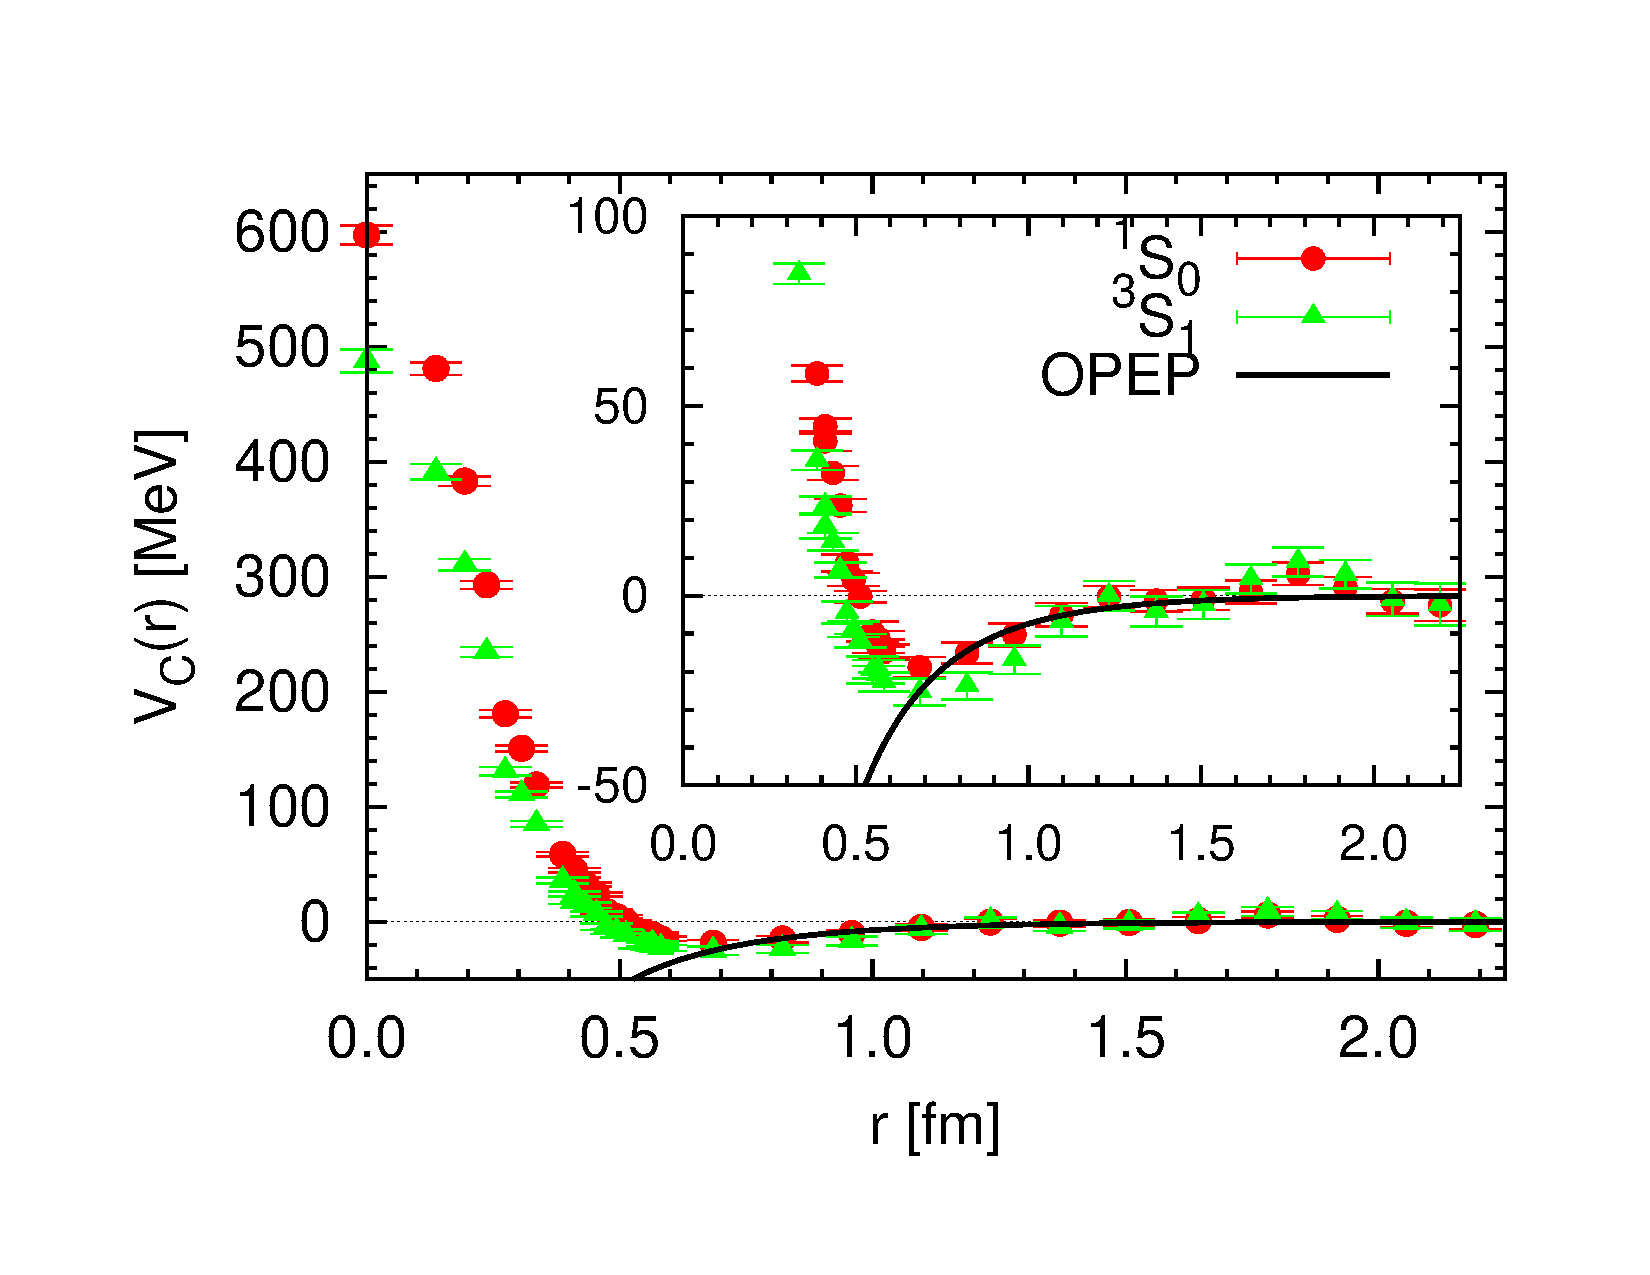
\includegraphics[width=0.45\columnwidth]{lattice}
  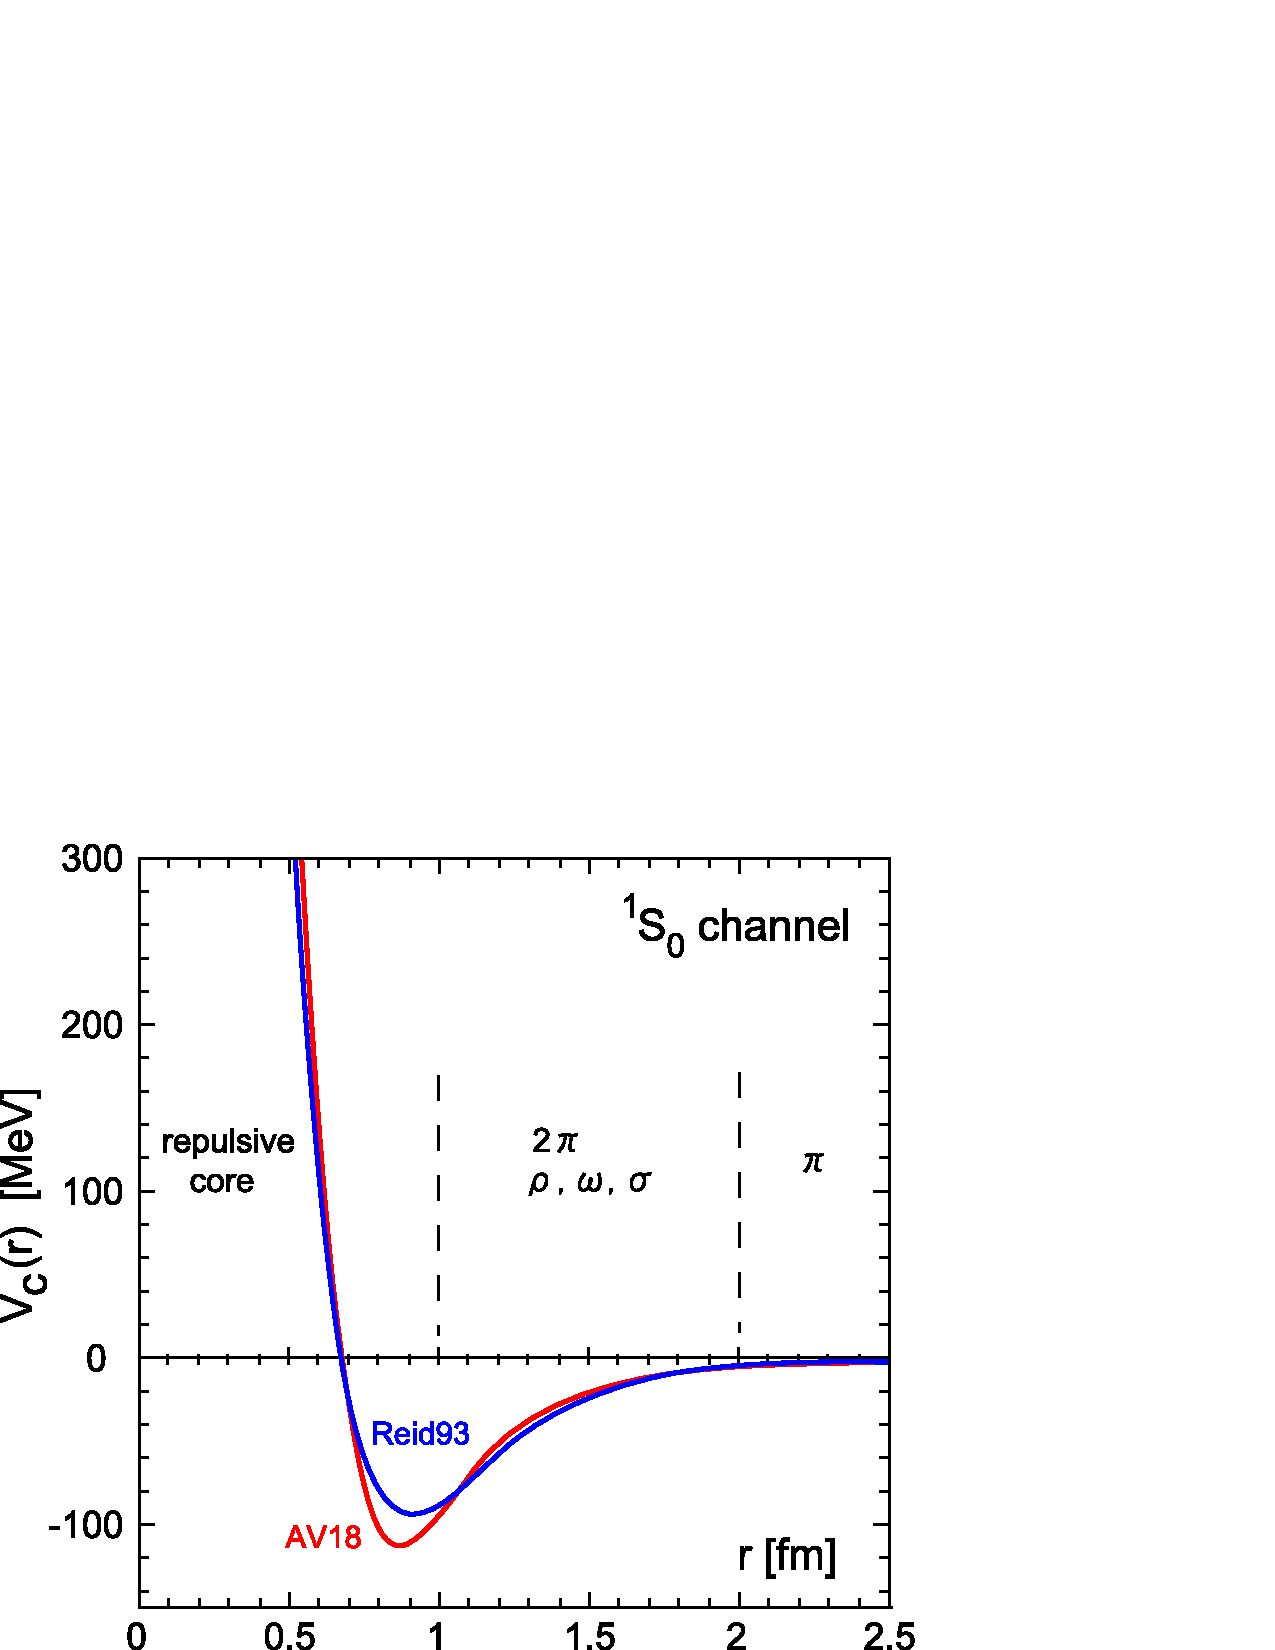
\includegraphics[width=0.45\columnwidth]{lattice1}\\[1ex]
\end{center}
The nucleon-nucleon interaction, Phenomenology vs Lattice calculations.
}





\frame
{
\frametitle{Features of the Nucleon-Nucleon (NN) Force}
The aim is to give you an overview over central features of the nucleon-nucleon interaction and how
it is constructed, with both technical and theoretical approaches. 
\begin{enumerate}
\item The existence of the deuteron with $J^{\pi}=1^+$ indicates that the force between protons and neutrons is attractive
at least for the $^3S_1$ partial wave. Interference between Coulomb and nuclear scattering for the proton-proton
partial wave $^1S_0$ shows that  the NN force is attractive at least for the $^1S_0$ partial wave. 
\item It has a short range and strong intermediate attraction.
\item Spin dependent, scattering lengths for triplet and singlet states are different,
\item Spin-orbit force. Observation of large polarizations of scattered nucleons perpendicular to the plane of scattering.
\end{enumerate}
} 
\frame
{
\frametitle{Features of the Nucleon-Nucleon (NN) Force, continued}
\begin{enumerate}
\item Strongly repulsive core. The $s$-wave phase shift becomes negative at $\approx 250$ MeV implying that the singlet $S$
has a hard core with range $0.4-0.5$ fm. 
\item Charge independence (almost). Two nucleons in a given two-body state always (almost) experience the same
force. Modern interactions break charge and isospin symmetry lightly. That means that the pp, neutron-neutron and pn 
parts of the 
interaction will be different for the same quantum numbers. 
\item Non-central. There is a tensor force. First indications from the quadrupole moment of the deuteron pointing to an
admixture in the ground state of both $l=2$ ($^3D_1$) and $l=0$ ($^3S_1$) orbital momenta.
\end{enumerate}
} 



\frame
{
\frametitle{Short Range Evidence}
Comparison of the binding energies of
$^2$H (deuteron), $^3$H (triton), $^4$He (alpha - particle)
  show that the nuclear force is of finite range ($1-2$ fm) and
  very strong within that range.
For nuclei with $A>4$, the energy saturates: Volume
  and binding energies of nuclei are proportional to the
  mass number $A$ (as we saw from exercise 1).

Nuclei are also bound. The average distance
between nucleons in nuclei is about $2$ fm which
must roughly correspond to the range of the
attractive part.
} 


\frame
{
\frametitle{Charge Dependence}
\begin{itemize}
\item  After correcting for the electromagnetic interaction, the forces
  between nucleons (pp, nn, or np) in the same state are almost the
  same.
\item  "Almost the same": Charge-independence is slightly broken.
\item  Equality between the pp and nn forces: Charge symmetry.
\item  Equality between pp/nn force and np force: Charge independence.
\item Better notation: Isospin symmetry, invariance under rotations in isospin
\end{itemize}
} 



\frame
{
\frametitle{Charge Dependence, $^1S_0$ Scattering Lengths}
Charge-symmetry breaking (CSB), after electromagnetic effects
have been removed:
\begin{itemize}
\item $a_{pp}=  -17.3 \pm 0.4 \hspace{0.cm} \mathrm{fm}$
\item $a_{nn}=-18.8 \pm 0.5 \hspace{0.cm} \mathrm{fm}$. Note however discrepancy from $nd$ breakup reactions
resulting in  $a_{nn}=-18.72 \pm 0.13 \pm 0.65 \hspace{0.cm} \mathrm{fm}$
and $\pi^- + d \rightarrow \gamma + 2n$ reactions giving  $a_{nn}=-18.93 \pm 0.27 \pm 0.3 \hspace{0.cm} \mathrm{fm}$.
\end{itemize}
Charge-independence breaking (CIB)
\begin{itemize}
\item $a_{pn}=  -23.74 \pm 0.02 \hspace{0.cm} \mathrm{fm}$ 
\end{itemize}
} 



\frame
{
\frametitle{Symmetries of the Nucleon-Nucleon (NN) Force}
\begin{enumerate}
\item Translation invariance
\item Galilean invariance
\item  Rotation invariance in space
\item Space reflection invariance
\item Time reversal invariance
\item Invariance under the interchange of particle $1$ and $2$
\item Almost isospin symmetry
\end{enumerate}
} 




\frame
{
\vspace{1cm}
\begin{columns}
\column{5.5cm}
% \begin{block}{$^1S_0$ Partial Wave}
%\begin{figure}
%\includegraphics[scale=0.5]{dean_hjorthjensen_fig02}
%\end{figure}
\begin{pgfpicture}{-2.25cm}{0.5cm}{5cm}{0.5cm}
   {\pgfbox[center,center]{\pgfuseimage{dean_hjorthjensen_fig02}}}
\end{pgfpicture}
% \end{block}
\column{5.5cm}
% \begin{block}{$^3P_2$ Partial Wave}
\begin{pgfpicture}{-2.25cm}{0.5cm}{5cm}{0.5cm}
   {\pgfbox[center,center]{\pgfuseimage{dean_hjorthjensen_fig05}}}
\end{pgfpicture}
%\begin{figure}
%\includegraphics[scale=0.5]{dean_hjorthjensen_fig05}
%\end{figure}
% \end{block}
\end{columns}
\vspace{1cm}
\[
V({\bf r})= \left\{ C_c + C_\sigma 
\mbox{\boldmath $\sigma$}_1\cdot\mbox{\boldmath $\sigma$}_2
 + C_T \left( 1 + {3\over m_\alpha r} + {3\over
\left(m_\alpha r\right)^2}\right) S_{12} (\hat r)\right. 
\]
\[
\left. + C_{SL} \left( {1\over m_\alpha r} + {1\over \left( m_\alpha r\right)^2}
\right) {\bf L}\cdot {\bf S}
\right\} \frac{e^{-m_\alpha r}}{m_\alpha r}
\]
How do we derive such terms?  This will be the aim for our lectures till spring break. (Note: no isospin dependence)
} 



\frame{
  \frametitle<presentation>{References for Various Phenomenological Interactions}
 Potentials which are based upon the standard non-relativistic operator structure
 are called "Phenomenological Potentials"
Some historically important examples are   
  \beamertemplatebookbibitems
    \begin{thebibliography}{10}
   \bibitem{ref1}     Gammel-Thaler potential ( Phys. Rev. {\bf 107}, 291, 1339 (1957) and the 
 Hamada-Johnston potential, Nucl. Phys. {\bf 34}, 382 (1962)), bot with a hard core.
    core.
   \bibitem{ref2}  Reid potential (Ann. Phys. (N.Y.) {\bf 50}, 411 (1968)), soft core.
\bibitem{ref3}   
Argonne $V_{14}$ potential (Wiringa et al., Phys. Rev. C {\bf 29}, 1207
    (1984)) with 14 operators and  the  Argonne $V_{18}$ potential (Wiringa et al., Phys. Rev. C {\bf 51}, 38
    (1995)), uses 18 operators
\bibitem{ref4}  A good reference: R.~Machleidt, Adv.~Nucl.~Phys~{\bf 19}, 189 (1989).
\end{thebibliography}
}



%\subsection{Developing Models for the NN force}

\frame
{
  \frametitle{Effective Degrees of Freedom, History}
\begin{enumerate}
\item From 1950 till approximately 2000: One-Boson-Exchange (OBE) models dominate. These are models which typically include several low-mass mesons, that is with masses below 1 GeV.
\item Now: models based on chiral perturbation theory. These are effective models with nucleons and pions as degrees of freedom only. The other mesons which appeared in standard one-boson model appear as multi-pion resonances. 
\end{enumerate}
}








\frame
{
\frametitle{Quantum numbers and the Sch\"odinger equation in relative and CM coordinates}
\begin{small}
{\scriptsize
Last week we discussed single-particle quantum numbers and two-particle quantum numbers.
For the single-particle case, we have the following eigenfunctions 
\[
\psi_{njm_j;ls}=\sum_{m_lm_s}\langle lm_lsm_s|jm_j\rangle\phi_{nlm_lsm_s},
\]
where the coefficients $\langle lm_lsm_s|jm_j\rangle$ are the so-called Clebsch-Gordan coeffficients.
The relevant quantum numbers are $n$ (related to the principal quantum number and the number of nodes of the wave function) and 
\[
   \OP{j}^2\psi_{njm_j;ls}=\hbar^2j(j+1)\psi_{njm_j;ls},
\]
\[
   \OP{j}_z\psi_{njm_j;ls}=\hbar m_j\psi_{njm_j;ls},
\]
\[
   \OP{l}^2\psi_{njm_j;ls}=\hbar^2l(l+1)\psi_{njm_j;ls},
\]
\[
   \OP{s}^2\psi_{njm_j;ls}=\hbar^2s(s+1)\psi_{njm_j;ls},
\]
but $s_z$ and $l_z$ do not result in good quantum numbers in a basis where we
use the angular momentum $j$.
}
\end{small}
}

\frame
{
\frametitle{Quantum numbers and the Sch\"odinger equation in relative and CM coordinates}
\begin{small}
{\scriptsize
For a two-body state where we couple two angular momenta $j_1$ and $j_2$ to a final
angular momentum $J$ with projection $M_J$, we can define a similar transformation in terms
of the Clebsch-Gordan coeffficients
\[
\psi_{(j_1j_2)JM_J}=\sum_{m_{j_1}m_{j_2}}\langle j_1m_{j_1}j_2m_{j_2}|JM_J\rangle\psi_{n_1j_1m_{j_1};l_1s_1}\psi_{n_2j_2m_{j_2};l_2s_2}.
\]
We will write these functions in a more compact form hereafter, namely,
\[
|(j_1j_2)JM_J\rangle=\psi_{(j_1j_2)JM_J},
\]
and 
\[
|j_im_{j_i}\rangle=\psi_{n_ij_im_{j_i};l_is_i},
\]
where we have skipped the explicit reference to $l$, $s$ and $n$. The spin of a nucleon is always $1/2$ while the value of $l$ can be deduced from the parity of the state.
It is thus normal to label a state with a given total angular momentum as 
$j^{\pi}$, where $\pi=\pm 1$. 
}
\end{small}
}


\frame
{
\frametitle{Quantum numbers and the Sch\"odinger equation in relative and CM coordinates}
\begin{small}
{\scriptsize
Our two-body state can thus be written as 
\[
|(j_1j_2)JM_J\rangle=\sum_{m_{j_1}m_{j_2}}\langle j_1m_{j_1}j_2m_{j_2}|JM_J\rangle|j_1m_{j_1}\rangle|j_2m_{j_2}\rangle.
\]
Due to the coupling order of the Clebsch-Gordan coefficient it reads as 
$j_1$ coupled to $j_2$ to yield a final angular momentum $J$. If we invert the order of coupling we would have
\[
|(j_2j_1)JM_J\rangle=\sum_{m_{j_1}m_{j_2}}\langle j_2m_{j_2}j_1m_{j_1}|JM_J\rangle|j_1m_{j_1}\rangle|j_2m_{j_2}\rangle,
\]
and due to the symmetry properties of the Clebsch-Gordan coefficient we have
\[
|(j_2j_1)JM_J\rangle=(-1)^{j_1+j_2-J}\sum_{m_{j_1}m_{j_2}}\langle j_1m_{j_1}j_2m_{j_2}|JM_J\rangle|j_1m_{j_1}\rangle|j_2m_{j_2}\rangle=(-1)^{j_1+j_2-J}|(j_1j_2)JM_J\rangle.
\]

We call the basis $|(j_1j_2)JM_J\rangle$ for the {\bf coupled basis}, or just $j$-coupled basis/scheme. The basis formed by the simple product of single-particle eigenstates 
$|j_1m_{j_1}\rangle|j_2m_{j_2}\rangle$ is called the {\bf uncoupled-basis}, or just the $m$-scheme basis. 
}
\end{small}
}


\frame
{
\frametitle{Quantum numbers}
\begin{small}
{\scriptsize
We have thus the coupled basis 
\[
|(j_1j_2)JM_J\rangle=\sum_{m_{j_1}m_{j_2}}\langle j_1m_{j_1}j_2m_{j_2}|JM_J\rangle|j_1m_{j_1}\rangle|j_2m_{j_2}\rangle.
\]
and the uncoupled basis 
\[
|j_1m_{j_1}\rangle|j_2m_{j_2}\rangle.
\]
The latter can easily be generalized to many single-particle states whereas the first 
needs specific coupling coefficients and definitions of coupling orders. 
The $m$-scheme basis is easy to implement numerically and is used in most standard shell-model codes. 
Our coupled basis obeys also the following relations
\[
   \OP{J}^2|(j_1j_2)JM_J\rangle=\hbar^2J(J+1)|(j_1j_2)JM_J\rangle
\]
\[
   \OP{J}_z|(j_1j_2)JM_J\rangle=\hbar M_J|(j_1j_2)JM_J\rangle,
\]
}
\end{small}
}


\frame
{
\frametitle{Relative and CoM system}
\begin{small}
{\scriptsize
What follows now is a more technical discussion of how we can solve the two-nucleon problem.
This will lead us to the so-called Lippman-Schwinger equation for the scattering problem and a rewrite of Schr\"odinger's equation in relative and center-of-mass coordinates. 

Let us define the latter first. As we did earlier this semester, we define
the center-of-mass (CoM)  momentum as
 \[
    \vec{K}=\sum_{i=1}^A\vec{k}_i,
 \]
with $\hbar=c=1$ the wave number $k_i=p_i$, with $p_i$ the pertinent momentum of a single-particle state. 
We have also the relative momentum
\[
    \vec{k}_{ij}=\frac{1}{2}(\vec{k}_i-\vec{k}_j).
 \]
We will below skip the indices $ij$ and simply write $\vec{k}$

 In a similar fashion we can define the CoM coordinate
 \[
     \vec{R}=\frac{1}{A}\sum_{i=1}^{A}\vec{r}_i,
 \]
 and the relative distance 
\[
    \vec{r}_{ij}=(\vec{r}_i-\vec{r}_j).
 \]
}
\end{small}
}


\frame
{
\frametitle{Relative and CoM system}
\begin{small}
{\scriptsize
With the definitions
 \[
    \vec{K}=\sum_{i=1}^A\vec{k}_i,
 \]
and 
\[
    \vec{k}_{ij}=\frac{1}{2}(\vec{k}_i-\vec{k}_j).
 \]
we can rewrite the two-particle kinetic energy (note that we use $\hbar=c=1$ as 
\[
\frac{\vec{k}_1^2}{2m_n}+\frac{\vec{k}_2^2}{2m_n}=\frac{\vec{k}^2}{m_n}+\frac{\vec{K}^2}{4m_n},
\]
where $m_n$ is the average of the proton and the neutron masses. 
Since the two-nucleon interaction depends only on the relative distance, this means that we can separate Schr\"odinger's equation in an equation for the center-of-mass motion and one for the relative motion.
}
\end{small}
}


\frame
{
\frametitle{Relative and CoM system}
\begin{small}
{\scriptsize
With an equation for the relative motion only and a separate one for the center-of-mass motion we need to redefine the two-body quantum numbers.

Previously we had a two-body state vector defined as $|(j_2j_1)JM_J\rangle$ in a coupled basis. 
We will now define the quantum numbers for the relative motion. Here we need to define new orbital momenta (since these are the quantum numbers which change). 
We define 
\[
\OP{l}_1+\OP{l}_2=\OP{\lambda}=\OP{l}+\OP{L},
\]
where $\OP{l}$ is the orbital momentum associated with the relative motion and
$\OP{L}$ the corresponding one linked with the CoM. The total spin $S$ is unchanged since it acts in a different space. We have thus that
\[
\OP{J}=\OP{l}+\OP{L}+\OP{S},
\]
which allows us to define the angular momentum of the relative motion
\[
{ \cal J} =  \OP{l}+\OP{S},
\]
where ${ \cal J}$ is the total angular momentum of the relative motion.
}
\end{small}
}

\frame
{
\frametitle{How to construct a nucleon-nucleon force: Mathematical Intermezzo, two-body Schr\"odinger in $k$-space}
\begin{small}
{\scriptsize
Before we break down the Schr\"odinger equation into a partial wave decomposition, we derive now the so-called Lippman-Schwinger equation. We will do this in an operator form first.
Thereafter, we rewrite it in terms of various quantum numbers such as relative momenta, orbital momenta etc. 
The Schr\"odinger equation in abstract vector representation is
\[
  \left( \hat{H}_0 + \hat{V} \right) \vert \psi_n \rangle = E_n \vert\psi_n \rangle. 
\]
In our case for the two-body problem $\hat{H}_0$ is just the kinetic energy. 
We rewrite it as 
\[
\left( \hat{H}_0 -E_n \right)\vert\psi_n \rangle =-\hat{V}\vert \psi_n \rangle . 
\]
We assume that the invers of $\left( \hat{H}_0 -E_n\right)$ exists and rewrite this equation as
\[
\vert\psi_n \rangle =\frac{1}{\left( E_n -\hat{H}_0\right)}\hat{V}\vert \psi_n \rangle . 
\]
}
\end{small}
}


\frame
{
\frametitle{How to construct a nucleon-nucleon force: Mathematical Intermezzo, two-body Schr\"odinger in $k$-space}
\begin{small}
{\scriptsize
The equation
\[
\vert \psi_n \rangle =\frac{1}{\left( E_n -\hat{H}_0\right)}\hat{V}\vert \psi_n \rangle,
\]
is normally solved in an iterative fashion. 
We assume first that
\[
\vert\psi_n \rangle = \vert\phi_n \rangle,
\] 
where $\vert\phi_n \rangle$ are the eigenfunctions of 
\[
\hat{H}_0\vert \phi_n \rangle=\omega_n\vert \phi_n \rangle
\]
the so-called unperturbed problem. In our case, these will simply be the kinetic energies of the relative motion. 
}
\end{small}
}



\frame
{
\frametitle{How to construct a nucleon-nucleon force: Mathematical Intermezzo, two-body Schr\"odinger in $k$-space}
\begin{small}
{\scriptsize
Inserting  $\vert\phi_n \rangle$  on the right-hand side of 
\[
\vert \psi_n \rangle =\frac{1}{( E_n -\hat{H}_0)}\hat{V}\vert \psi_n \rangle,
\]
yields
\[
\vert \psi_n \rangle =\vert\phi_n \rangle+\frac{1}{\left( E_n -\hat{H}_0\right)}\hat{V}\vert \phi_n \rangle,
\]
as our first iteration. 
Reinserting again gives
\[
\vert \psi_n \rangle =\vert\phi_n \rangle+\frac{1}{\left( E_n -\hat{H}_0\right)}\hat{V}\vert \phi_n \rangle+\frac{1}{( E_n -\hat{H}_0)}\hat{V}\frac{1}{\left( E_n -\hat{H}_0\right)}\hat{V}\vert \phi_n \rangle,
\]
and continuing we obtain
\[
\vert \psi_n \rangle =\sum_{i=0}^{\infty}\left[\frac{1}{( E_n -\hat{H}_0)}\hat{V}\right]^i\vert \phi_n \rangle.
\]
}
\end{small}
}


\frame
{
\frametitle{How to construct a nucleon-nucleon force: Mathematical Intermezzo, two-body Schr\"odinger in $k$-space}
\begin{small}
{\scriptsize
It is easy to see that 
\[
\vert \psi_n \rangle =\sum_{i=0}^{\infty}\left[\frac{1}{(E_n -\hat{H}_0)}\hat{V}\right]^i\vert \phi_n \rangle,
\]
can be rewritten as 
\[
\vert \psi_n \rangle =\vert\phi_n \rangle+\frac{1}{( E_n -\hat{H}_0)}
\hat{V}\left(1+ \frac{1}{(E_n -\hat{H}_0)}\hat{V}+\frac{1}{(E_n -\hat{H}_0)}\hat{V}\frac{1}{(E_n -\hat{H}_0)}\hat{V}+\dots\right]\vert \phi_n \rangle,
\]
which we rewrite as 
\[
\vert \psi_n \rangle =\vert\phi_n \rangle+\frac{1}{(E_n -\hat{H}_0)}\hat{V}\vert \psi_n \rangle.
\]


}
\end{small}
}



\frame
{
\frametitle{How to construct a nucleon-nucleon force: Mathematical Intermezzo, two-body Schr\"odinger in $k$-space}
\begin{small}
{\scriptsize
In operator form we have thus
\[
\vert \psi_n \rangle =\vert\phi_n \rangle+\frac{1}{(E_n -\hat{H}_0)}\hat{V}\vert \psi_n \rangle.
\]
We multiply from the left with $\hat{V}$ and $\langle \phi_m \vert$ and obtain
\[
\langle \phi_m \vert\hat{V}\vert \psi_n \rangle =\langle \phi_m \vert\hat{V}\vert\phi_n \rangle+\langle \phi_m \vert\hat{V}\frac{1}{(E_n -\hat{H}_0)}\hat{V}\vert \psi_n \rangle.
\]
We define thereafter the so-called $T$-matrix as
\[
\langle \phi_m \vert\hat{T}\vert \phi_n \rangle=\langle \phi_m \vert\hat{V}\vert \psi_n \rangle.
\]
We can rewrite our equation as
\[
\langle \phi_m \vert\hat{T}\vert \phi_n \rangle =\langle \phi_m \vert\hat{V}\vert\phi_n \rangle+\langle \phi_m \vert\hat{V}\frac{1}{(E_n -\hat{H}_0)}\hat{T}\vert \phi_n \rangle.
\]


}
\end{small}
}



\frame
{
\frametitle{How to construct a nucleon-nucleon force: Mathematical Intermezzo, two-body Schr\"odinger in $k$-space}
\begin{small}
{\scriptsize
The equation
\[
\langle \phi_m \vert\hat{T}\vert \phi_n \rangle =\langle \phi_m \vert\hat{V}\vert\phi_n \rangle+\langle \phi_m \vert\hat{V}\frac{1}{(E_n -\hat{H}_0)}\hat{T}\vert \phi_n \rangle,
\]
is called the Lippman-Schwinger equation. Inserting the completeness relation
\[ 
{\bf 1} = \sum_n \vert \phi_n\rangle\langle \phi_n \vert, \:\: \langle \phi_n\vert \phi_{n'} \rangle = \delta_{n,n'}
\]
we have 
\[
\langle \phi_m \vert\hat{T}\vert \phi_n \rangle =\langle \phi_m \vert\hat{V}\vert\phi_n \rangle+\sum_k \langle \phi_m \vert\hat{V}\vert \phi_k\rangle\frac{1}{(E_n -\omega_k)}\langle \phi_k \vert\hat{T}\vert \phi_n \rangle,
\]
which is (when we specify the state $\vert\phi_n \rangle$) an integral equation that can actually be solved by matrix inversion easily! The unknown quantity is the $T$-matrix.

}
\end{small}
}







\frame
{
\frametitle{How to construct a nucleon-nucleon force: Mathematical Intermezzo, two-body Schr\"odinger in $k$-space}
\begin{small}
{\scriptsize
Now we wish to introduce a partial wave decomposition in order to solve the Lippman-Schwinger equation. With a partial wave decomposition we can reduce a three-dimensional integral equation to a one-dimensional one. 

Let us continue with our Schr\"odinger equation in the abstract vector representation
\begin{equation}
  \left( T + V \right) \vert \psi_n \rangle = E_n \vert\psi_n \rangle 
  \label{eq:vec_rep}
\end{equation}
Here $T$ is the kinetic energy operator and $V$ is the potential operator. 
The eigenstates form a complete orthonormal set according to 
\[ 
{\bf 1} = \sum_n \vert \psi_n\rangle\langle \psi_n \vert, \:\: \langle \psi_n\vert \psi_{n'} \rangle = \delta_{n,n'}
\]
}
\end{small}
}




\frame
{
\frametitle{Mathematical Intermezzo, two-body Schr\"odinger in $k$-space}
\begin{small}
{\scriptsize
The most commonly used representations of equation~\ref{eq:vec_rep} are the coordinate
and
the momentum space representations. They define the completeness relations 
\begin{eqnarray}
 {\bf 1}&  = &  \int d{\bf r} \:\vert  {\bf r} \rangle \langle {\bf r}\vert, \:\: 
 \langle  {\bf r}\vert  {\bf r'} \rangle = \delta ( {\bf r}-{\bf r'}) \\
{\bf 1} & = & \int d{\bf k} \:\vert  {\bf k} \rangle \langle {\bf k}\vert, \:\: 
  \langle  {\bf k}\vert  {\bf k'} \rangle = \delta ( {\bf k}-{\bf k'}) 
\end{eqnarray}
Here the basis states in  both ${\bf r}$- and ${\bf k}$-space are dirac-delta 
function normalized. From this it follows that the plane-wave states are given by,
\begin{equation}
  \langle  {\bf r}\vert  {\bf k} \rangle = \left( 1\over2\pi \right)^{3/2}\exp \left( i {\bf k\cdot r} \right)
  \label{eq:planewave1}
\end{equation}
which is a transformation function defining the mapping from the abstract 
$ \vert {\bf k} \rangle $ to the abstract $\vert {\bf r}\rangle $ space.
}
\end{small}
}




\frame
{
\frametitle{Mathematical Intermezzo, two-body Schr\"odinger in $k$-space}
\begin{small}
{\scriptsize
That the ${\bf r}$-space basis states are 
delta-function normalized follows from 
\begin{equation}
  \delta ( {\bf r}-{\bf r'}) = \langle {\bf r} \vert {\bf r}'\rangle = 
  \langle {\bf r} \vert {\bf 1} \vert {\bf r}'\rangle = 
  \int \mathrm{d}{\bf k} \langle {\bf r}\vert {\bf k} \rangle \langle {\bf k}\vert {\bf r}' \rangle = 
  \left( {1\over 2\pi}\right)^3 \int \mathrm{d}{\bf k} e^{i {\bf k}({\bf r} - {\bf r}')} 
\end{equation}
and the same for the momentum space basis states,
\begin{equation}
  \delta ( {\bf k}-{\bf k'}) = \langle {\bf k} \vert {\bf k}'\rangle = 
  \langle {\bf k} \vert {\bf 1} \vert {\bf k}'\rangle = 
  \int \mathrm{d}{\bf r} \langle {\bf k}\vert {\bf r} \rangle \langle {\bf r}\vert {\bf k}' \rangle = 
  \left( {1\over 2\pi}\right)^3 \int \mathrm{d}{\bf r} e^{i {\bf r}({\bf k} - {\bf k}')} 
\end{equation}
}
\end{small}
}




\frame
{
\frametitle{Mathematical Intermezzo, two-body Schr\"odinger in $k$-space}
\begin{small}
{\scriptsize
Projecting equation~(\ref{eq:vec_rep}) on momentum states
the momentum space Schr\"odinger equation is obtained,
\begin{equation}
  {\hbar^2 \over 2\mu} k^2 \psi_n({\bf k})  + 
  \int d{\bf k'}\: V({\bf k}, {\bf k'}) \psi_n({\bf k'}) = 
  E_n \psi_n({\bf k})
  \label{eq:momspace1}
\end{equation}
Here the notation $\psi_n({\bf k}) = \langle {\bf k} \vert \psi_n\rangle $ and 
$ \langle {\bf k} \vert V \vert {\bf k}' \rangle = V({\bf k}, {\bf k'})$ has been introduced.
The potential in momentum space is given by a double Fourier-transform 
of the potential in coordinate space, i.e.
\begin{equation} 
  V ({\bf k}, {\bf k'}) = \left( {1\over 2\pi}\right)^3 \int \mathrm{d}{\bf r}\int \mathrm{d}{\bf r}'\: 
  e^{-i {\bf kr} }V({\bf r},{\bf r}') e^{i{\bf k}'{\bf r}'}  
\end{equation}
}
\end{small}
}




\frame
{
\frametitle{Mathematical Intermezzo, two-body Schr\"odinger in $k$-space}
\begin{small}
{\scriptsize
Here it is assumed that the potential interaction does not contain any spin dependence. 
Instead of a differential equation in coordinate space, the Schr\"odinger
equation becomes an integral equation in momentum space. This has 
many tractable features. Firstly, most realistic 
nucleon-nucleon interactions derived from field-theory are given 
explicitly in momentum space. Secondly, the boundary conditions imposed
on the differential equation in coordinate space are automatically built into the
integral equation. And last, but not least, integral equations are easy to numerically 
implement, and convergence is obtained by just increasing the number of integration
points.
Instead of solving the three-dimensional integral equation given in equation~(\ref{eq:momspace1}), an 
infinite set of 1-dimensional equations can be obtained via a  partial wave
expansion. 
}
\end{small}
}



\frame
{
\frametitle{Mathematical Intermezzo, two-body Schr\"odinger in $k$-space}
\begin{small}
{\scriptsize
The wave function $ \psi_n({\bf k}) $ can be expanded in a complete set of spherical harmonics, i.e. 
\begin{equation}
  \psi_n({\bf k}) = \sum _{lm} \psi_{nlm}(k)Y_{lm} (\hat{k}), \:\:
  \psi_{nlm}(k) = \int d\hat{k} Y_{lm}^*(\hat{k})\psi_n({\bf k}).   
  \label{eq:part_wave1}
\end{equation}
By inserting equation~\ref{eq:part_wave1} in equation~\ref{eq:momspace1}, and projecting from the left
$Y_{lm}(\hat{k})$, the three-dimensional Schr\"odinger equation~(\ref{eq:momspace1}) is reduced
to an infinite set of  1-dimensional angular momentum coupled integral equations, 
\begin{equation}
  \left( {\hbar^2 \over 2\mu} k^2 - E_{nlm}\right) \psi_{nlm}(k) =  
  -\sum_{l'm'} \int_{0}^\infty dk' {k'}^2 V_{lm, l'm'}(k,k') \psi_{nl'm'}(k') 
  \label{eq:part_wave2}
\end{equation}
where the angular momentum projected potential takes the form,
\begin{equation}
  V_{lm, l'm'}(k,k') = \int \mathrm{d}{\hat{k}} \int \mathrm{d}{\hat{k}'}\: 
    Y_{lm}^*(\hat{k})V({\bf k}, {\bf k'})Y_{l'm'}(\hat{k}')
    \label{eq:pot1}
\end{equation}
here $\mathrm{d}{\hat k} = \mathrm{d}\theta \sin\theta \:\mathrm{d}\varphi $.
{\bf Note that we discuss only the orbital momentum, we will include angular momentum and spin later}. 
}
\end{small}
}




\frame
{
\frametitle{Mathematical Intermezzo, two-body Schr\"odinger in $k$-space}
\begin{small}
{\scriptsize
Often the potential is given in position space, so it is convenient to establish 
the connection between $V_{lm, l'm'}(k,k')$ and $V_{lm, l'm'}(r,r')$. Inserting 
position space completeness in equation~(\ref{eq:pot1}) gives
\begin{eqnarray}
\nonumber
  V_{lm, l'm'}(k,k')& = &\int \mathrm{d}{\bf{r}} \int \mathrm{d}{\bf{r}'}\: 
  \int \mathrm{d}{\hat{k}} \int \mathrm{d}{\hat{k}'}\: 
  Y_{lm}^*(\hat{k})\langle {\bf k}\vert {\bf r} \rangle
  \langle{\bf r}  \vert V \vert {\bf r}' \rangle
  \langle {\bf r'}\vert {\bf k}' \rangle Y_{lm}(\hat{k}') \\ \nonumber
  &=&\int \mathrm{d}{\bf{r}} \int \mathrm{d}{\bf{r}'}\: 
  \left\{ \int \mathrm{d}{\hat{k}}  Y_{lm}^*(\hat{k})\langle {\bf k}\vert {\bf r} \rangle \right\} \\
  &&\times\langle{\bf r}  \vert V \vert {\bf r}' \rangle
  \left\{ \int \mathrm{d}{\hat{k}'}\:   Y_{lm}(\hat{k}') \langle {\bf r'}\vert {\bf k}' \rangle\right\}
  \label{eq:pot2}
\end{eqnarray}
}
\end{small}
}



\frame
{
\frametitle{Mathematical Intermezzo, two-body Schr\"odinger in $k$-space}
\begin{small}
{\scriptsize
Since the plane waves depend only on the absolute values of position and momentum, 
$ \vert {\bf k} \vert, \vert {\bf r} \vert  $,
and the angle between them, $ \theta_{kr} $, they may be expanded in terms of bipolar harmonics of 
zero rank, i.e.  
\begin{equation} 
  e^{i {\bf k}\cdot {\bf r}} = 4\pi \sum_{l=0}^{\infty} i^l j_l(kr)\left( Y_l(\hat{k}) \cdot Y_l(\hat{r}) \right)
  = \sum_{l=0}^{\infty} (2l+1)i^l j_l(kr) P_l(\cos \theta_{kr}) 
\end{equation}
where the addition theorem for spherical harmonics has been used in order to write
the expansion in terms of Legendre polynomials. The spherical Bessel functions, $j_l(z)$,  
are given in terms of Bessel functions of the first kind with half integer orders,  
\[
j_l(z) = \sqrt{\pi \over 2 z} J_{l+1/2}(z).  
\]
}
\end{small}
}



\frame
{
\frametitle{Mathematical Intermezzo, two-body Schr\"odinger in $k$-space}
\begin{small}
{\scriptsize
Inserting the plane-wave expansion
into the brackets of equation~(\ref{eq:pot2}) yields, 
\begin{eqnarray}
  \nonumber
  \int \mathrm{d}{\hat{k}}  Y_{lm}^*(\hat{k})\langle {\bf k}\vert {\bf r} \rangle & = &  
  \left( {1\over 2\pi} \right) ^{3/2}4\pi i^{-l} j_l(kr) Y_{lm}^*(\hat{r}), \\  
  \nonumber
  \int \mathrm{d}{\hat{k}'}\:   Y_{lm}(\hat{k}') \langle {\bf r'}\vert {\bf k}' \rangle & = &  
  \left( {1\over 2\pi} \right) ^{3/2}4\pi i^{l'} j_{l'}(k'r') Y_{l'm'}(\hat{r}). 
\end{eqnarray}
}
\end{small}
}


\frame
{
\frametitle{Mathematical Intermezzo, two-body Schr\"odinger in $k$-space}
\begin{small}
{\scriptsize
The connection between the momentum- and position space angular momentum 
projected potentials are then given, 
\begin{equation}
  V_{lm, l'm'}(k,k') = {2 \over \pi} i^{l' -l}\int_0^\infty dr\: r^2 \int_0^\infty dr'\: {r'}^2 
  j_l(kr) V_{lm,l'm'}(r,r') j_{l'}(k'r')
  \label{eq:pot3}
\end{equation}
which is known as a double Fourier-Bessel transform. The position space angular 
momentum projected potential is given by
\begin{equation}
  V_{lm, l'm'}(r,r') = \int \mathrm{d}{\hat{r}} \int \mathrm{d}{\hat{r}'}\: 
  Y_{lm}^*(\hat{r})V({\bf r}, {\bf r'})Y_{l'm'}(\hat{r}').
  \label{eq:pot4}
\end{equation}
}
\end{small}
}



\frame
{
\frametitle{Mathematical Intermezzo, two-body Schr\"odinger in $k$-space}
\begin{small}
{\scriptsize
No assumptions of locality/non-locality and deformation of the interaction has so far been made, 
and the result in equation~(\ref{eq:pot3}) is general. In position space the Schr\"odinger equation 
takes form of an integro-differential equation in case of a non-local interaction, 
in momentum space the Schr\"odinger equation is an ordinary integral equation of the Fredholm type, 
see equation~(\ref{eq:part_wave2}). This is a further advantage of the momentum space approach as compared to 
the standard position space approach.  
If we assume that the 
interaction is of local character, i.e. 
\begin{equation}
  \nonumber
  \langle {\bf r}\vert V \vert {\bf r'}\rangle = V({\bf r}) \delta( {\bf r}-{\bf r}' ) = 
  V({\bf r}) {\delta( { r}-{r}' ) \over r^2} \delta ( \cos \theta - \cos \theta' ) \delta (\varphi-\varphi'), 
\end{equation}
then equation~(\ref{eq:pot4}) reduces to 
\begin{equation}
  V_{lm, l'm'}(r,r') = {\delta( { r}-{r}' ) \over r^2}\int \mathrm{d}{\hat{r}}\:
  Y_{lm}^*(\hat{r})V({\bf r})Y_{l'm'}(\hat{r}),
  \label{eq:pot5}
\end{equation}
}
\end{small}
}



\frame
{
\frametitle{Mathematical Intermezzo, two-body Schr\"odinger in $k$-space}
\begin{small}
{\scriptsize
and equation~(\ref{eq:pot3}) reduces to  
\begin{equation}
  V_{lm, l'm'}(k,k') = {2 \over \pi} i^{l' -l}\int_0^\infty dr\: r^2 \:
  j_l(kr) V_{lm,l'm'}(r) j_{l'}(k'r)
  \label{eq:pot6}
\end{equation}
where 
\begin{equation}
  V_{lm, l'm'}(r) = \int \mathrm{d}{\hat{r}}\:
  Y_{lm}^*(\hat{r})V({\bf r})Y_{l'm'}(\hat{r}),
  \label{eq:pot10}
\end{equation}
}
\end{small}
}


\frame
{
\frametitle{Mathematical Intermezzo, two-body Schr\"odinger in $k$-space}
\begin{small}
{\scriptsize
In the case that the interaction is central, $V({\bf r}) = V(r)$, then
\begin{equation}
  V_{lm, l'm'}(r) = V(r) \int \mathrm{d}{\hat{r}}\:
  Y_{lm}^*(\hat{r})Y_{l'm'}(\hat{r}) = V(r) \delta_{l,l'}\delta_{m,m'},
  \label{eq:pot7}
\end{equation}
and 
\begin{equation}
  V_{lm, l'm'}(k,k') = {2 \over \pi} \int_0^\infty dr\: r^2 \:
  j_l(kr) V(r) j_{l'}(k'r)\delta_{l,l'}\delta_{m,m'} = 
  V_l(k,k') \delta_{l,l'}\delta_{m,m'}
  \label{eq:pot8}
\end{equation}
where the momentum space representation of the interaction finally reads,
\begin{equation}
  V_{l}(k,k') = {2 \over \pi} \int_0^\infty dr\: r^2 \:
  j_l(kr) V(r) j_{l}(k'r).
  \label{eq:pot9}
\end{equation}
}
\end{small}
}



\frame
{
\frametitle{Mathematical Intermezzo, two-body Schr\"odinger in $k$-space}
\begin{small}
{\scriptsize
For a local and spherical symmetric potential, 
the coupled momentum space Schr\"odinger equations given in equation~(\ref{eq:part_wave2})
decouples in angular momentum, 
giving
\begin{equation}
  {\hbar^2 \over 2\mu} k^2 \psi_{n l}(k) + 
  \int_{0}^\infty dk' {k'}^2 V_{l}(k,k') \psi_{n l }(k') =
  E_{n l} \psi_{n l}(k) 
  \label{eq:momentum_space}
\end{equation}   
Where we have written $\psi_{n l }(k) = \psi_{nlm}(k)$, since the 
equation becomes independent of the projection $m$ for spherical symmetric interactions. 
The momentum space wave functions $\psi_{n l}(k) $ defines a complete orthogonal set 
of functions, which spans the space of functions with a positive finite Euclidean norm 
 (also called $l^2$-norm), $ \sqrt{ \langle \psi_n \vert \psi_n \rangle} $, which 
is a Hilbert space. The corresponding normalized wave function in coordinate space
is given by the Fourier-Bessel transform 
\begin{equation}
  \phi_{n l}(r)  = \sqrt{ 2\over \pi}\int dk\: k^2 j_l(kr) \psi_{n l}(k)
\end{equation}    
}
\end{small}
}



\frame
{
\frametitle{How to construct the force: Partial wave expansion of the nuclear force}

\begin{small}
{\scriptsize
We will thus assume that the interaction is spherically symmetric and use
the partial wave expansion of the plane waves in
terms of spherical harmonics.
This means that we can separate the radial part of the wave function from its
angular dependence. The wave function of the relative motion is described
in terms of plane waves as
\begin{equation}
       e^{\imath {\bf kr}}  =
       \bra{\bf r}{\bf k}\rangle =  4\pi \sum_{lm} \imath ^{l}
        j_{l} (kr) Y_{lm}^{*}({\bf \hat{k}}) Y_{lm}({\bf \hat{r}}),
\end{equation}
where $j_l$ is a spherical Bessel function and $Y_{lm}$ the
spherical harmonics.
}
\end{small}
}


\frame
{
\frametitle{First Solution Step}
\begin{small}
{\scriptsize
In terms of the relative and center-of-mass momenta ${\bf k}$ and
${\bf K}$, the potential in momentum space is related to the nonlocal operator
$V({\bf r},{\bf r}')$ by
\[
      \bra{{\bf k'K'}}V \ket{{\bf kK}} =
       \int d {\bf r}d {\bf r'}
        e^{-\imath {\bf k'r'}}V({\bf r'},{\bf r}) e^{\imath {\bf kr}}
       \delta({\bf K},{\bf K'}).
\]
We will assume that the interaction is spherically symmetric.
Can separate the radial part of the wave function from its
angular dependence. The wave function of the relative motion is described
in terms of plane waves as
\[
       e^{\imath {\bf kr}}  =
       \bra{\bf r}{\bf k}\rangle =  4\pi \sum_{lm} \imath ^{l}
        j_{l} (kr) Y_{lm}^{*}({\bf \hat{k}}) Y_{lm}({\bf \hat{r}}),
\]
where $j_l$ is a spherical Bessel function and $Y_{lm}$ the
spherical harmonic.
}
\end{small}

}


\frame
{
\frametitle{How to construct the force: Partial wave expansion of the nuclear force}

\begin{small}
{\scriptsize
This partial wave basis is useful for defining the operator for
the nucleon-nucleon interaction, which
is symmetric with respect to rotations, parity and
isospin transformations. These symmetries imply that the interaction is
diagonal with respect to the quantum numbers of total relative angular
momentum ${\cal J}$, spin $S$ and isospin $T$ (we skip isospin for the moment). Using the above plane wave expansion,
and coupling to final ${\cal J}$ and $S$ and $T$ we get
\[
      \bra{{\bf k'}} V \ket{{\bf k}}
       = (4\pi)^2 \sum_{STll'm_lm_{l'}{\cal J}}
      \imath ^{l+l'} Y_{lm}^{*}({\bf \hat{k}}) Y_{l'm'}({\bf \hat{k}'})
\]
\[
      \langle lm_lSm_S|{\cal J}M\rangle \langle l'm_{l'}Sm_S|{\cal J}M\rangle          
      \bra{k'l'S{\cal J}M}V \ket{klS{\cal J}M},
\]
where we have defined
\begin{equation}
    \bra{k'l'S{\cal J}M}V \ket{klS{\cal J}M}=
    \int   j_{l'}(k'r')\bra{l'S{\cal J}M}V(r',r)\ket{lS{\cal J}M}j_l(kr) {r'}^2 dr' r^2 dr.
\end{equation}
We have omitted the momentum of the center-of-mass motion ${\bf K}$ and the 
corresponding orbital momentum $L$, since the interaction is diagonal
in these variables.
}
\end{small}
}

\frame
{
\frametitle{The Lippman-Schwinger equation in a partial wave expansion}
\begin{small}
{\scriptsize
We wrote the Lippman-Schwinger equation as
\[
\langle \phi_m \vert\hat{T}\vert \phi_n \rangle =\langle \phi_m \vert\hat{V}\vert\phi_n \rangle+\sum_k \langle \phi_m \vert\hat{V}\vert \phi_k\rangle\frac{1}{(E_n -\omega_k)}\langle \phi_k \vert\hat{T}\vert \phi_n \rangle.
\]
How do we rewrite it in a partial wave expansion with momenta $k$?
}
\end{small}
}




\frame
{
\begin{small}
{\scriptsize

The general structure of the $T$-matrix in partial waves is
\[
   T_{ll'}^{\alpha}(kk'K\omega)=V_{ll'}^{\alpha}(kk')
\]
\[
   +{\displaystyle \frac{2}{\pi}\sum_{l''m_{l''}M_S}\int_{0}^{\infty} d {\bf q}
   (\langle l''m_{l''}Sm_S|{\cal J}M\rangle)^2
   \frac{Y_{l''m_{l''}}^*(\hat{{\bf q}})
   Y_{l''m_{l''}}(\hat{{\bf q}}) V_{ll''}^{\alpha}(kq)
   T_{l''l'}^{\alpha}(qk'K\omega)}
   {\omega -H_0}},
   \label{eq:bspartial}
\]
The  shorthand notation
\[
    T_{ll'}^{\alpha}(kk'K\omega)=
   \bra{kKlL{\cal J}S}T(\omega)\ket{k'Kl'L{\cal J}S},
\]
denotes the $T$-matrix
with momenta $k$ and $k'$ and orbital momenta $l$ and $l'$
of the relative motion, and
$K$ is the corresponding momentum of
the center-of-mass motion. Further, $L$, ${\cal J}$, $S$ and $T$
are the orbital momentum of the center-of-mass motion, the
total angular momentum,
spin and isospin, respectively. 
Due to the nuclear tensor force (to be discussed later), the interaction is not diagonal in $ll'$.
}
\end{small}

}

\frame
{
\begin{small}
{\scriptsize

Using the orthogonality
properties of the Clebsch-Gordan coefficients and the spherical harmonics,
we obtain the well-known
one-dimensional angle independent
integral equation
\[
   T_{ll'}^{\alpha}(kk'K\omega)=V_{ll'}^{\alpha}(kk')
   +\frac{2}{\pi}\sum_{l''}\int_{0}^{\infty} dqq^2
   \frac{V_{ll''}^{\alpha}(kq)
   T_{l''l'}^{\alpha}(qk'K\omega)}
   {\omega -H_0}.
\]
Inserting the denominator we arrive at 
\[
   \hat{T}_{ll'}^{\alpha}(kk'K)=\hat{V}_{ll'}^{\alpha}(kk')
   +\frac{2}{\pi}\sum_{l''}\int_{0}^{\infty} dqq^2
   \hat{V}_{ll''}^{\alpha}(kq)
   \frac{1}{k^2-q^2 +i\epsilon}
   \hat{T}_{l''l'}^{\alpha}(qk'K).
\]
}
\end{small}

}


\frame
{
\frametitle{How do we construct the interaction: Lippman-Schwinger Equation}
\begin{small}
{\scriptsize
To parameterize the nucleon-nucleon interaction we solve the Lippman-Scwhinger
equation
\[
   T_{ll'}^{\alpha}(kk'K)=V_{ll'}^{\alpha}(kk')
   +\frac{2}{\pi}\sum_{l''}\int_{0}^{\infty} dqq^2
   V_{ll''}^{\alpha}(kq)
   \frac{1}{k^2-q^2 +i\epsilon}
   T_{l''l'}^{\alpha}(qk'K).
\]
The  shorthand notation
\[
    T(\hat{V})_{ll'}^{\alpha}(kk'K\omega)=
   \bra{kKlL{\cal J}S}T(\omega)\ket{k'Kl'L{\cal J}S},
\]
denotes the $T(V)$-matrix
with momenta $k$ and $k'$ and orbital momenta $l$ and $l'$
of the relative motion, and
$K$ is the corresponding momentum of
the center-of-mass motion. Further, $L$, ${\cal J}$, and $S$
are the orbital momentum of the center-of-mass motion, the
total angular momentum and
spin, respectively. We skip for the moment isospin.
}
\end{small}
}

\frame
{
\frametitle{Numerical Solution}
\begin{small}
{\scriptsize


For scattering states, the energy is positive, $E>0$. 
The Lippman-Schwinger equation (a rewrite of the Schr\"odinger equation)
is an integral equation
where we have to deal with the amplitude 
$R(k,k')$ (reaction matrix, which is the real part of  the full
complex $T$-matrix)
defined through the integral equation for one partial wave (no coupled-channels) 
\[
    R_l(k,k') = V_l(k,k') +\frac{2}{\pi}{\cal P}
                \int_0^{\infty}dqq^2V_l(k,q)\frac{1}{E-q^2/m}R_l(q,k').
   \label{eq:ls1}
\]
For negative energies (bound states) and intermediate states scattering states blocked
by  occupied states below the Fermi level.

}
\end{small}
}


\frame
{
\frametitle{Relation to data}
\begin{small}
{\scriptsize

The symbol ${\cal P}$ in the previous slide indicates that Cauchy's principal-value prescription
is used in order to avoid the singularity arising from the zero of the denominator.


The total kinetic energy of the two 
incoming particles in the center-of-mass system
is 
\[
    E=\frac{k_0^2}{m_n}.
\]


The matrix $R_l(k,k')$ relates to the 
the  phase shifts through its diagonal elements as
\[
     R_l(k_0,k_0)=-\frac{tan\delta_l}{mk_0}.
     \label{eq:shifts}
\]
}
\end{small}

}

\frame
{
\frametitle{Recipe I, possible topic for project 2}
\begin{small}
{\scriptsize
{\bf This material is optional, but could define a possible project 2}.

From now on we will drop the subscript $l$ in all equations.
In order to solve the Lippman-Schwinger equation 
in momentum space, we need first to write 
a function which sets up the mesh points. 
We need to do that since we are going to approximate an integral
through 
\[
   \int_a^bf(x)dx\approx\sum_{i=1}^Nw_if(x_i),
\]
where we have fixed $N$ lattice points through the corresponding weights
$w_i$ and points $x_i$. Typically obtained via methods like Gaussian quadrature.
}
\end{small}

}


\frame
{
\frametitle{Recipe II}
\begin{small}
{\scriptsize

If you use Gauss-Legendre the points are determined for the interval $x_i\in [-1,1]$
You map these points over to the limits in your integral. You can then
use the following mapping
        \[
          k_i=const\times tan\left\{\frac{\pi}{4}(1+x_i)\right\},
        \]
and 
         \[
            \omega_i= const\frac{\pi}{4}\frac{w_i}{cos^2\left(\frac{\pi}{4}(1+x_i)\right)}.
         \]
If you choose units fm$^{-1}$ for $k$, set $const=1$. If you choose to work
with MeV, set $const\sim 200$ ($\hbar c=197$ MeVfm).
}
\end{small}

}


\frame
{
\frametitle{Recipe III}
\begin{small}
{\scriptsize

The principal value integral is rather tricky
to evaluate numerically, mainly since computers have limited
precision. We will here use a subtraction trick often used
when dealing with singular integrals in numerical calculations.
We introduce first the calculus relation
\[
  \int_{-\infty}^{\infty} \frac{dk}{k-k_0} =0.
\]
It means that the curve $1/(k-k_0)$ has equal and opposite
areas on both sides of the singular point $k_0$. If we break
the integral into one over positive $k$ and one over 
negative $k$, a change of variable $k\rightarrow -k$ 
allows us to rewrite the last equation as
\[
  \int_{0}^{\infty} \frac{dk}{k^2-k_0^2} =0.
\]
}
\end{small}

}


\frame
{
\frametitle{Recipe IV}
\begin{small}
{\scriptsize

We can then express a principal values integral
as
\[
  {\cal P}\int_{0}^{\infty} \frac{f(k)dk}{k^2-k_0^2} =
  \int_{0}^{\infty} \frac{(f(k)-f(k_0))dk}{k^2-k_0^2},
   \label{eq:trick}
\]
where the right-hand side is no longer singular at 
$k=k_0$, it is proportional to the derivative $df/dk$,
and can be evaluated numerically as any other integral.
}
\end{small}

}


\frame
{
\frametitle{Recipe V}
\begin{small}
{\scriptsize

We can then use this trick to obtain
\[
    R(k,k') = V(k,k') +\frac{2}{\pi}
                \int_0^{\infty}dq
                \frac{q^2V(k,q)R(q,k')-k_0^2V(k,k_0)R(k_0,k')  }
                     {(k_0^2-q^2)/m}.
   \label{eq:ls2}
\]
This is the equation to solve numerically in order
to calculate the phase shifts. We are interested in obtaining
$R(k_0,k_0)$.
}
\end{small}

}


\frame
{
\frametitle{Recipe VI}
\begin{small}
{\scriptsize

How do we proceed?

Using the mesh points $k_j$ and the weights $\omega_j$,
         we reach
\[
          R(k,k') = V(k,k') +\frac{2}{\pi}
          \sum_{j=1}^N\frac{\omega_jk_j^2V(k,k_j)R(k_j,k')}
                           {(k_0^2-k_j^2)/m}
           -\frac{2}{\pi}k_0^2V(k,k_0)R(k_0,k')
          \sum_{n=1}^N\frac{\omega_n}
                           {(k_0^2-k_n^2)/m}.                
\]
}
\end{small}

}


\frame
{
\frametitle{Recipe VII}
\begin{small}
{\scriptsize

This equation contains now the unknowns $R(k_i,k_j)$
(with dimension $N\times N$) and $R(k_0,k_0)$.

We can turn it into an equation
with dimension $(N+1)\times (N+1)$ with  a mesh
which contains the original mesh points $k_j$ for $j=1,N$
and the point which corresponds to the energy $k_0$.
Consider the latter as the 'observable' point.
The mesh points become then $k_j$ for $j=1,n$ and
$k_{N+1}=k_0$. 

With these new mesh points we define the matrix
\[
      A_{i,j}=\delta_{i,j}-V(k_i,k_j)u_j,
      \label{eq:aeq}
\]
}
\end{small}

}



\frame
{
\frametitle{Recipe VIII}
\begin{small}
{\scriptsize

where $\delta$ is the Kronecker $\delta$
and
\[
     u_j=\frac{2}{\pi}
         \frac{\omega_jk_j^2}{(k_0^2-k_j^2)/m}\hspace{1cm}
         j=1,N
\]
and
\[
     u_{N+1}=-\frac{2}{\pi}
          \sum_{j=1}^N\frac{k_0^2\omega_j}{(k_0^2-k_j^2)/m}.
\]
}
\end{small}

}


\frame
{
\frametitle{Recipe IX}
\begin{small}
{\scriptsize

The first task is then to 
set up the matrix $A$ for a given $k_0$. This is an
$(N+1)\times (N+1)$ matrix. It can be convenient
to have an outer loop which runs over the chosen
observable values for the energy $k_0^2/m$.
{\em Note that all mesh points $k_j$ for $j=1,N$ must be
different from $k_0$. Note also that
$V(k_i,k_j)$ is an
$(N+1)\times (N+1)$ matrix}. 

  With the matrix $A$ we can rewrite the problem
  as a matrix problem of dimension $(N+1)\times (N+1)$.
  All matrices $R$, $A$ and $V$ have this dimension
  and we get
\[
    A_{i,l}R_{l,j}=V_{i,j},
\] 
or just
\[
    AR=V.
\] 
}
\end{small}

}


\frame
{
\frametitle{Recipe X}
\begin{small}
{\scriptsize

Since you already have defined $A$ and $V$
(these are stored as $(N+1)\times (N+1)$ matrices) 
The final equation involves only the unknown
$R$. We obtain it by matrix inversion, i.e.,
\[
    R=A^{-1}V.
    \label{eq:final2}
\] 
Thus, to obtain $R$, you will need to set up the matrices
$A$ and $V$ and invert the matrix $A$. 
With the inverse $A^{-1}$, perform
a matrix multiplication with $V$ results in $R$.


With $R$ you can then evaluate the phase shifts
by noting that 
\[
      R(k_{N+1},k_{N+1})=R(k_0,k_0)=-\frac{tan\delta}{mk_0},
\]
where $\delta$ are the phase shifts.
}
\end{small}

}

\frame
{
\frametitle{Phase shifts}
\begin{small}
{\scriptsize

For elastic scattering, the scattering potential can only change the outgoing spherical wave function up to a phase. In the asymptotic limit, far away from the scattering potential, we get for the spherical bessel function
\[
j_l(kr) \xrightarrow[]{ r \gg 1} \frac{\sin(kr -l\pi/2)}{kr} =  \frac{1}{2ik}\left( \frac{e^{i(kr-l\pi/2)}}{r} - \frac{e^{-i(kr-l\pi/2)}}{r}\right)
\]
The outgoing wave will change by a phase shift $\delta_l$, from which we can define the S-matrix $S_l(k) = e^{2i\delta_l(k)}$. Thus, we have
\[
 \frac{e^{i(kr-l\pi/2)}}{r} \xrightarrow[]{\textnormal{phase change}}  \frac{S_l(k)e^{i(kr-l\pi/2)}}{r}
\]
}
\end{small}

}

\frame
{
\frametitle{Cross section}
\begin{small}
{\scriptsize

The solution to the Schrodinger equation for a spherically symmetric potential, will have the form
\[
\psi_k(r) = e^{ikr} + f(\theta)\frac{e^{ikr}}{r}
\]
where $f(\theta)$ is the scattering amplitude, and related to the differential cross section as
\[
\frac{d\sigma}{d\Omega} = |f(\theta)|^2
\]
Using the expansion of a plane wave in spherical waves, we can relate the scattering amplitude $f(\theta)$ with the partial wave phase shifts $\delta_l$ by identifying the outgoing wave 
\[
\psi_k(r) = e^{ikr} + \left[\frac{1}{2ik}\sum_l i^l (2l+1) (S_l(k)-1)P_l(\cos(\theta))e^{-il\pi/2}\right] \frac{e^{ikr}}{r}
\]
which can be simplified further by cancelling $i^l$ with $e^{-il\pi/2}$ 
}
\end{small}

}

\frame{
\frametitle{Cross section}
\begin{small}
{\scriptsize

From the previous slide we have
\[
\psi_k(r) = e^{ikr} + f(\theta) \frac{e^{ikr}}{r}
\]
with 
\[
f(\theta) = \sum_l (2l+1)f_l(\theta) P_l(\cos(\theta))
\]
where the partial wave scattering amplitude is given by
\[
f_l(\theta) = \frac{1}{k}\frac{(S_l(k)-1)}{2i} = \frac{1}{k}\sin\delta_l(k) e^{i\delta_l(k)}
\]
With Eulers formula for the cotanget, this can also be written as
\[
f_l(\theta) = \frac{1}{k}\frac{1}{\cot \delta_l(k) - i}
\]
}
\end{small}

}

\frame
{
\frametitle{Meaning of the phase shift}
\begin{center}
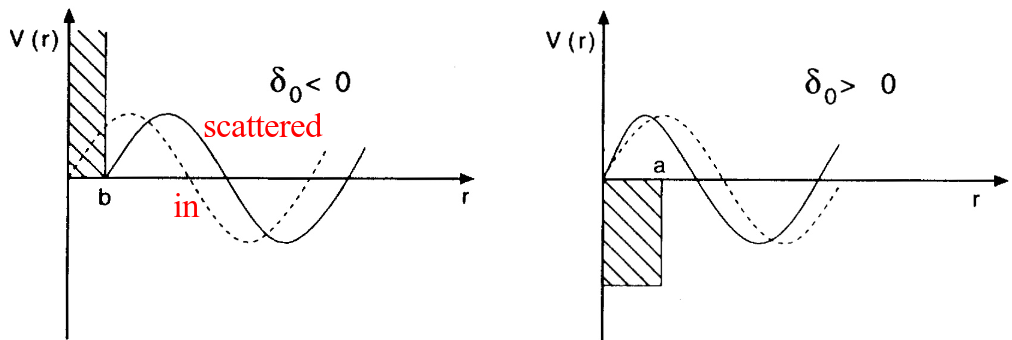
\includegraphics[width=11cm]{./phase.png}
\end{center}
}

\frame{
\frametitle{Cross Section}
\begin{small}
{\scriptsize

The integrated cross section is given by
\begin{align}
\begin{split}
\sigma = {}& 2\pi \int_0^{\pi} |f(\theta)|^2 \sin \theta\, \textnormal{d}\theta = \\
{}& = 2\pi \sum_l |\frac{(2l+1)}{k} \sin \delta_l |^2 \int_0^{\pi} (P_l(\cos \theta))^2 \sin \theta\, \textnormal{d}\theta = \\
{}& = \frac{4\pi}{k^2} \sum_l (2l+1) \sin^2\delta_l(k) = 4\pi \sum_l (2l+1)|f_l(\theta)|^2 
\end{split}
\end{align}
Where the orthogonality of the Legendre polynomials was used to evaluate the last integral
\[
\int_0^{\pi} P_l(\cos \theta)^2 \sin \theta \, \textnormal{d}\theta = \frac{2}{2l+1}
\]
Thus, the \textit{total} cross section is the sum of the partial-wave cross sections. Note that the differential cross section contains cross-terms from different partial waves. The integral over the full sphere enables the use of the legendre orthogonality, and this kills the cross-terms.
}
\end{small}

}

\frame
{
\frametitle{Low energy scattering: the scattering length}
\begin{small}
{\scriptsize

At low energy, $k \rightarrow 0$, S-waves are most important. In this region we can define the scattering length $a$ and the effective range $r$. The $S-$wave scattering amplitude is given by
\[
f_l(\theta) = \frac{1}{k}\frac{1}{\cot \delta_l(k) - i}
\]
Taking the limit $k \rightarrow 0$, gives us the expansion
\[
k \cot \delta_0 = -\frac{1}{a} + \frac{1}{2}r_0 k^2 + \ldots
\]
Thus the low energy cross section is given by
\[
\sigma = 4\pi a^2
\]
If the system contains a bound state, the scattering length will become positive (neutron-proton in $^3S_1$). For the $^1S_0$ wave, the scattering length is negative and large. This indicates that the wave function of the system is at the verge of turning over to get a node, but cannot create a bound state in this wave.%\\
%(\url{http://people.ccmr.cornell.edu/~emueller/well.html})
}
\end{small}

}

\frame
{
\frametitle{Low energy scattering: the scattering length}
\begin{center}
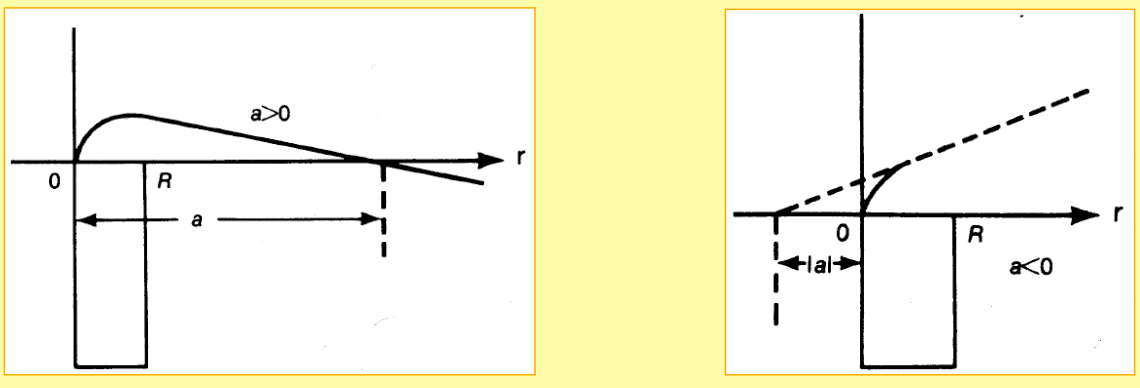
\includegraphics[width=11cm]{./scattering_length.png}
\end{center}
}

\frame{
\frametitle{How to extract phase shifts}
\begin{small}
{\scriptsize
It is important to realize that the phase shifts themselves aren't observables. The measurable scattering quantity is the cross section, or the differential cross section. The partial wave phase shifts can be thought of as a parameterization of the (experimental) cross sections. The phase shifts provide insights into the physics of partial wave projected nuclear interactions, and are thus important quantities to know.\\The nucleon-nucleon differential cross section have been measured at almost all energies up to the pion production threshold (290 MeV in the Lab frame), and this experimental data base is what provides us with the constraints on our nuclear interaction models. In order to pin down the unknown coupling constants of the theory, a statistical optimization with respect to cross sections need to be carried out. This is how we constraint the nucleon-nucleon interaction in practice!
}
\end{small}

}

\frame
{
\frametitle{Nijmegen multi-energy $pp$ PWA phase shifts}
\begin{center}
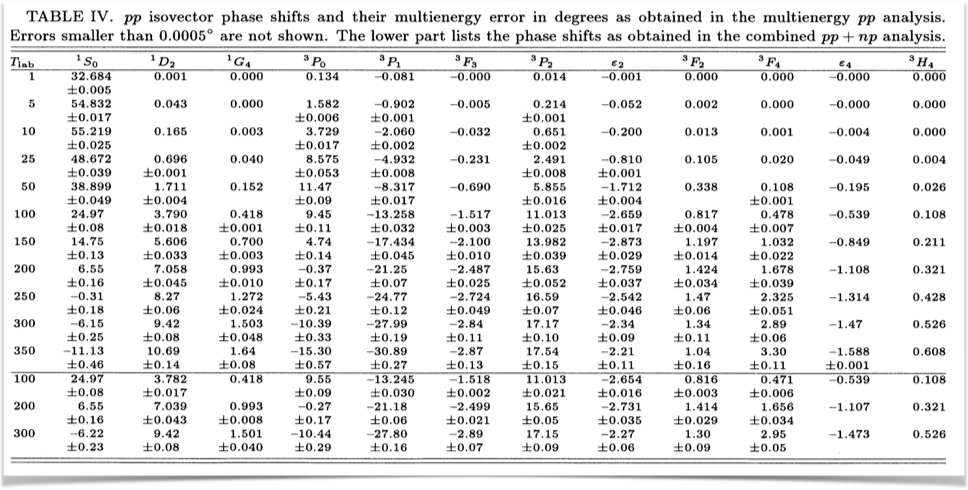
\includegraphics[width=9.5cm]{./nijmegen_pp_phase_shifts.png}
\end{center}
The $pp$-data is more accurate than the $np$-data, and for $nn$ there is no data. The quality of a potential is gauged by the $\chi^2$/datum with respect to the scattering data base
}

\frame
{
\frametitle{np-$\chi^2$/datum for some potentials}
\begin{center}
\begin{tabular}{ccccc} \hline \hline
$T_{\textnormal{lab}}$ bin (MeV) &  N3LO$^1$     & NNLO$^2$   & NLO$^2$  & AV18$^3$   \\ 
                             &          &        &      &         \\ \hline 
0-100                        &  1.05    & 1.7    & 4.5  & 0.95    \\
100-190                      &  1.08    & 22     & 100  & 1.10    \\
190-290                      &  1.15    & 47     & 180  & 1.11    \\ \hline
{\bf 0-290}                   &  \textbf{1.10}    & \textbf{20}     & \textbf{86}   & \textbf{1.04}    \\ \hline \hline 
\end{tabular}
\end{center}
\begin{enumerate}
\item R. Machleidt et al., Phys. Rev. C68, 041001(R) (2003)\\
\item E. Epelbaum et al., Eur. Phys. J. A19, 401 (2004)\\
\item R. B. Wiringa et al., Phys. Rev. C5, 38 (1995)
\end{enumerate}
}

\frame
{
\frametitle{An example: chiral twobody interactions}
\begin{block}{Chiral effective Lagrangian.}
\[
\mathcal{L_{\textnormal{eff}}} = \mathcal{L}_{\pi \pi}(f_\pi,m_{\pi}) + \mathcal{L}_{\pi N}(f_{\pi},M_{N},g_A,c_i,d_i,...) + \mathcal{L}_{NN}(C_{i},\tilde{C}_{i},D_{i},...) + \ldots
\]
\begin{tiny}
R. Machleidt, D. R. Entem, Phys. Rep. 503, 1 (2011)\\E. Epelbaum, H.-W. Hammer, Ulf-G. Mei\ss{}ner, Rev. Mod. Phys. 81, 1773 (2009)
\end{tiny}
\end{block}
}

\frame
{
\frametitle{Phase shift}
pn-$^1S_0$ phase shift. Note that the Nijm93 PWA phase shift becomes negative at T$_{\textnormal{lab}}> 250$MeV. This indicates that the nucleon-nucleon potential is repulsive at short distances 
\begin{center}
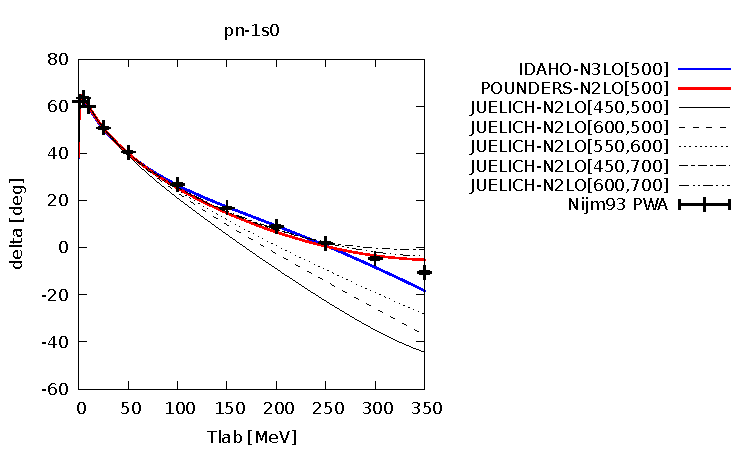
\includegraphics[width=11.0cm]{./phase-pn-1s0_IDAHO_JUELICH.pdf}
\end{center}
}

\frame
{
\frametitle{Differential cross section}
\begin{center}
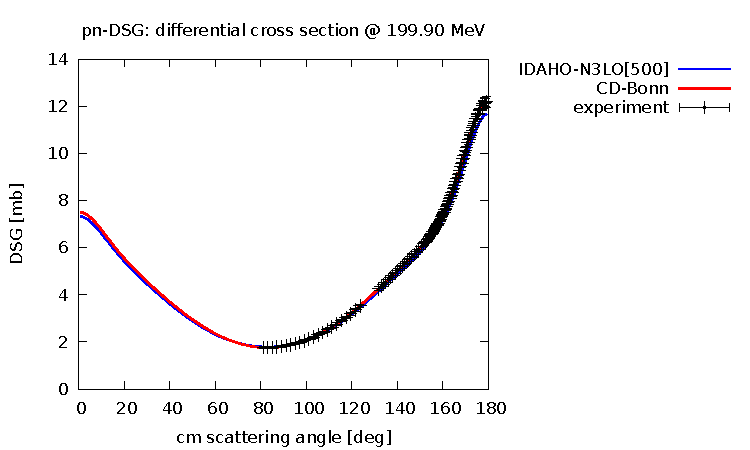
\includegraphics[width=11.0cm]{./pnDSG_at_199MeV.pdf}
\end{center}
}

\section[Week 9]{Week 9}

\frame
{
  \frametitle{Topics for Week 9, February 24-28}
  \begin{block}{Nuclear forces}
\begin{itemize}
\item Monday:
\item Repetion from last week
\item Phenomenology of nuclear forces and its quantum numbers (with isospin, part 1)
\item Wednesday:
\item How do we derive the force using nucleons and mesons like the pion? 
%\item Two-body Hamiltonians for nuclear structure studies (with isospin part 2). No slides yet for this part, see Alex Brown's lectures, chapter 19.
\end{itemize}
For a good discussion of isospin, see Alex Brown's lecture notes chapter 12, 13 and 19.  {\bf No lectures Friday 28.}
%Chapter 19, gives you also a good starting point for the discussion of the two-body Hamiltonian.


  \end{block}
} 

\frame
{
\frametitle{Symmetries of the Nucleon-Nucleon (NN) Force}
\begin{enumerate}
\item Translation invariance
\item Galilean invariance
\item  Rotation invariance in space
\item Space reflection invariance
\item Time reversal invariance
\item Invariance under the interchange of particle $1$ and $2$
\item Almost isospin symmetry
\end{enumerate}
} 




\frame
{
\frametitle{A typical form of the nuclear force}
Here we display a typical way to parametrize (non-relativistic expression) the nuclear two-body force
in terms of some operators, the central part, the spin-spin part and the central force.
\[
V({\bf r})= \left\{ C_c + C_\sigma 
\mbox{\boldmath $\sigma$}_1\cdot\mbox{\boldmath $\sigma$}_2
 + C_T \left( 1 + {3\over m_\alpha r} + {3\over
\left(m_\alpha r\right)^2}\right) S_{12} (\hat r)\right. 
\]
\[
\left. + C_{SL} \left( {1\over m_\alpha r} + {1\over \left( m_\alpha r\right)^2}
\right) {\bf L}\cdot {\bf S}
\right\} \frac{e^{-m_\alpha r}}{m_\alpha r}
\]
How do we derive such terms?  (Note: no isospin dependence and that the above is an approximation)
} 

\frame
{
  \frametitle{Warning}
  \begin{block}{Nuclear forces}
To derive the above famous form of the nuclear force using field theoretical concepts, we will need some 
elements from relativistic quantum mechanics. I know that many of you have not taken a course in quantum field theory. I hope however that you can see the basic ideas leading to the famous non-relativistic expressions for the nuclear force. \newline\newline
{\bf Furthermore, when we analyze nuclear data, we will actually try to explain properties like spectra, single-particle energies etc in terms of the various terms of the nuclear force. Moreover, many of you will hear about these terms at various talks, workshops, seminars etc. Then, it is good to have an idea of what people actually mean!!}
  \end{block}
} 

\frame
{
  \frametitle{Dramatis Personae}
\begin{center}
\begin{tabular}{llll} \\ \hline
\multicolumn{1}{c}{Baryons}&
\multicolumn{1}{c}{Mass (MeV)}&
\multicolumn{1}{c}{Mesons}&
\multicolumn{1}{c}{Mass (MeV)}
\\ \hline
$p,n$&938.926&$\pi$&138.03\\
$\Lambda$&1116.0&$\eta$&548.8\\
$\Sigma$&1197.3&$\sigma$&$\approx 550.0$\\
$\Delta$&1232.0&$\rho$&770\\
&&$\omega$&782.6\\
&&$\delta$&983.0\\
&&$K$&495.8\\
&&$K^{\star}$&895.0\\  \hline
\end{tabular}
\end{center}
}

\frame
{
\frametitle{Components of the force and quantum numbers}
But before we proceed, we will look into specific quantum numbers of the relative system and study 
expectation vaues of the various terms of
\[
V({\bf r})= \left\{ C_c + C_\sigma 
\mbox{\boldmath $\sigma$}_1\cdot\mbox{\boldmath $\sigma$}_2
 + C_T \left( 1 + {3\over m_\alpha r} + {3\over
\left(m_\alpha r\right)^2}\right) S_{12} (\hat r)\right. 
\]
\[
\left. + C_{SL} \left( {1\over m_\alpha r} + {1\over \left( m_\alpha r\right)^2}
\right) {\bf L}\cdot {\bf S}
\right\} \frac{e^{-m_\alpha r}}{m_\alpha r}
\]
} 




\frame
{
\frametitle{Components of the force and quantum numbers}
\begin{small}
{\scriptsize
The tensor force is given by
\[
S_{12} (\hat r) = \frac{3}{r^2}\left(\mbox{\boldmath $\sigma$}_1\cdot {\bf r}\right) \left(\mbox{\boldmath $\sigma$}_2\cdot {\bf r}\right) -\mbox{\boldmath $\sigma$}_1\cdot\mbox{\boldmath $\sigma$}_2\]
where the Pauli matrices are defined as
\[
\sigma_x =\begin{Bmatrix} 0 & 1 \\ 1 & 0 \end{Bmatrix},
\]
\[
\sigma_y =\begin{Bmatrix} 0 & -\imath \\ \imath & 0 \end{Bmatrix},
\]
and
\[
\sigma_z =\begin{Bmatrix} 1 & 0 \\ 0 & -1 \end{Bmatrix},
\]
with the properties $\sigma = 2{\bf S}$ (the spin of the system, being $1/2$ for nucleons), 
$\sigma^2_x=\sigma^2_y=\sigma_z={\bf 1}$ and
obeying the commutation and anti-commutation relations $\{\sigma_x,\sigma_y\} =0$
$[\sigma_x,\sigma_y] =\imath\sigma_z$ etc.
}
\end{small}

} 
\frame
{
\frametitle{Components of the force and quantum numbers}
\begin{small}
{\scriptsize
When we look at the expectation value of 
$\langle \mbox{\boldmath $\sigma$}_1\cdot\mbox{\boldmath $\sigma$}_2\rangle$, we can rewrite this expression in terms of the
spin ${\bf S}={\bf s}_1+{\bf s}_2$, resulting in 
\[
\langle\mbox{\boldmath $\sigma$}_1\cdot\mbox{\boldmath $\sigma$}_2\rangle=2(S^2-s_1^2-s_2^2)=2S(S+1)-3,
\]
where we $s_1=s_2=1/2$ leading to
\[
\left\{ \begin{array}{cc} \langle\mbox{\boldmath $\sigma$}_1\cdot\mbox{\boldmath $\sigma$}_2\rangle=1 &  \mathrm{if} \hspace{0.2cm} S=1\\
\langle\mbox{\boldmath $\sigma$}_1\cdot\mbox{\boldmath $\sigma$}_2\rangle=-3 & \mathrm{if} \hspace{0.2cm} S=0\\\end{array}\right.
\]
}
\end{small}

} 
\frame
{
\frametitle{Components of the force and quantum numbers}
\begin{small}
{\scriptsize
Similarly, the expectation value of the spin-orbit term is 
\[
\langle {\bf l}{\bf S} \rangle = \frac{1}{2}\left( {\cal J}({\cal J}+1)-l(l+1)-S(S+1)\right),
\]
which means that for $s$-waves with either $S=0$ and thereby ${\cal  J}=0$ or $S=1$ and ${\cal J}=1$, 
the expectation value for the
spin-orbit force is zero. With the above phenomenological model, the
only contributions to the expectation value of the potential energy for $s$-waves
stem  from the central and the spin-spin components since the
expectation value of the tensor force is also zero.
}
\end{small}

} 
\frame
{
\frametitle{Components of the force and quantum numbers}
 For $s=1/2$ spin values only for two nucleons, the expectation value of the tensor force operator is 
\begin{center}
\begin{tabular}{lccc} 
& & $l'$  &  \\ \hline
 & & & \\ 
$l$  & ${\cal J}+1$    & ${\cal J}$  & ${\cal J}-1$  \\ & & & \\  \hline 
& & & \\ 
${\cal J}+1$ & $-\frac{2{\cal J}({\cal J}+2)}{2{\cal J}+1}$  &0  &$\frac{6\sqrt{{\cal J}({\cal J}+1)}}{2{\cal J}+1}$   \\ 
& & & \\ 
${\cal J}$&  0      &2      &    0     \\ 
& & & \\ 
${\cal J}-1$& $\frac{6\sqrt{{\cal J}({\cal J}+1)}}{2{\cal J}+1}$       & 0     & $-\frac{2(2{\cal J}+1)}{2{\cal J}+1}$        \\
& & & \\ \hline 
\end{tabular}
\end{center}
We will derive these expressions after spring break, when we have discussed the Wigner-Eckart theorem. 
} 


\frame
{
\frametitle{Components of the force and isospin}
\begin{small}
{\scriptsize
 The nuclear forces are almost charge independent. If we assume they are, 
we can introduce a new quantum number which is conserved. For nucleons only, that is a proton and neutron, we can limit ourselves
to two possible values which allow us to distinguish between the two particles. If we assign an isospin value of $\tau=1/2$ for protons
and neutrons (they belong to an isospin doublet, in the same way as we discussed the spin $1/2$ multiplet), we can define 
the neutron to have isospin projection $\tau_z=+1/2$ and a proton to have $\tau_z=-1/2$. These assignements are the standard choices in low-energy nuclear physics.
}
\end{small}
}
\frame
{
\frametitle{Components of the force and isospin}
\begin{small}
{\scriptsize
This means that we can define a single-nucleon
state function in terms of the quantum numbers $n$, $j$, $m_j$, $l$, $s$, $\tau$ and $\tau_z$. Using our definitions in terms of an uncoupled basis, we had 
\[
\psi_{njm_j;ls}=\sum_{m_lm_s}\langle lm_lsm_s|jm_j\rangle\phi_{nlm_lsm_s},
\]
which we can now extend to
\[
\psi_{njm_j;ls}\xi_{\tau\tau_z}=\sum_{m_lm_s}\langle lm_lsm_s|jm_j\rangle\phi_{nlm_lsm_s}\xi_{\tau\tau_z},
\]
with the isospin spinors defined as 
\[
\xi_{\tau=1/2\tau_z=+1/2}=\left(\begin{array}{c} 1  \\ 0\end{array}\right),
\]
and
\[
\xi_{\tau=1/2\tau_z=-1/2}=\left(\begin{array}{c} 0  \\ 1\end{array}\right).
\]
We can then define the proton state function as 
\[
\psi^p({\bf r})  =\psi_{njm_j;ls}({\bf r})\left(\begin{array}{c} 0  \\ 1\end{array}\right), 
\]
and similarly for neutrons as
\[
\psi^n({\bf r})  =\psi_{njm_j;ls}({\bf r})\left(\begin{array}{c} 1  \\ 0\end{array}\right). 
\]
}
\end{small}
}

\frame
{
\frametitle{Components of the force and isospin}
\begin{small}
{\scriptsize
We can in turn define the isospin Pauli matrices as
\[
\hat{\tau}_x =\left(\begin{array}{cc} 0 & 1 \\ 1 & 0 \end{array}\right),
\]
\[
\hat{\tau}_y =\left(\begin{array}{cc} 0 & -\imath \\ \imath & 0 \end{array}\right),
\]
and
\[
\hat{\tau}_z =\left(\begin{array}{cc} 1 & 0 \\ 0 & -1 \end{array}\right),
\]
and operating with $\hat{\tau}_z$ on the proton state function we have
\[
\hat{\tau}_z\psi^p({\bf r})=-\frac{1}{2}\psi^p({\bf r}),
\]
and for neutrons we have
\[
\hat{\tau}\psi^n({\bf r})=\frac{1}{2}\psi^n({\bf r}).
\]
}
\end{small}
}

\frame
{
\frametitle{Components of the force and isospin}
\begin{small}
{\scriptsize
We can now define the so-called charge operator as 
\[
\frac{\hat{Q}}{e} = \frac{1}{2}\left(1-\hat{\tau}_z\right)=\begin{Bmatrix} 0 & 0 \\ 0 & 1 \end{Bmatrix},
\]
which results in 
\[
\frac{\hat{Q}}{e}\psi^p({\bf r})=\psi^p({\bf r}),
\]
and 
\[
\frac{\hat{Q}}{e}\psi^n({\bf r})=0,
\]
as it should be. 
}
\end{small}
}
\frame
{
\frametitle{Components of the force and isospin}
\begin{small}
{\scriptsize
The total isospin is defined as
\[
\hat{T}=\sum_{i=1}^A\hat{\tau}_i,
\]
and its corresponding isospin projection as
\[
\hat{T}_z=\sum_{i=1}^A\hat{\tau}_{z_i},
\]
with eigenvalues $T(T+1)$ for $\hat{T}$ and $1/2(N-Z)$ for $\hat{T}_z$, where $N$ is the number of neutrons and $Z$ the number of protons. 

If charge is conserved, the Hamiltonian $\hat{H}$ commutes with $\hat{T}_z$ and all members of a given isospin multiplet
(that is the same value of $T$) have the same energy and there is no $T_z$ dependence and we say that $\hat{H}$ is a scalar in isospin space.
}
\end{small}
}
\frame
{
\frametitle{Components of the force and isospin}
\begin{small}
{\scriptsize
If we now add isospin to our simple $V_4$ interaction model, we end up with $8$ operators, popularly dubbed $V_8$ interaction model. The explicit form reads
\[
V({\bf r})= \left\{ C_c + C_\sigma 
\mbox{\boldmath $\sigma$}_1\cdot\mbox{\boldmath $\sigma$}_2
 + C_T \left( 1 + {3\over m_\alpha r} + {3\over
\left(m_\alpha r\right)^2}\right) S_{12} (\hat r)\right. 
\]
\[
\left. + C_{SL} \left( {1\over m_\alpha r} + {1\over \left( m_\alpha r\right)^2}
\right) {\bf L}\cdot {\bf S}
\right\} \frac{e^{-m_\alpha r}}{m_\alpha r}
\]
\[
+ \left\{ C_{c\tau} + C_{\sigma\tau} 
\mbox{\boldmath $\sigma$}_1\cdot\mbox{\boldmath $\sigma$}_2
 + C_{T\tau} \left( 1 + {3\over m_\alpha r} + {3\over
\left(m_\alpha r\right)^2}\right) S_{12} (\hat r)\right. 
\]
\[
\left. + C_{SL\tau} \left( {1\over m_\alpha r} + {1\over \left( m_\alpha r\right)^2}
\right) {\bf L}\cdot {\bf S}
\right\}\mbox{\boldmath $\tau$}_1\cdot\mbox{\boldmath $\tau$}_2 \frac{e^{-m_\alpha r}}{m_\alpha r}
\]
}
\end{small}
}
\frame
{
\frametitle{Components of the force and isospin}
\begin{small}
{\scriptsize
The expectation value of 
$\langle \mbox{\boldmath $\tau$}_1\cdot\mbox{\boldmath $\tau$}_2\rangle$ is calculated along the same lines as we did for
the two spin matrices and we obtain
\[
\left\{ \begin{array}{cc} \langle\mbox{\boldmath $\sigma$}_1\cdot\mbox{\boldmath $\sigma$}_2\rangle\langle\mbox{\boldmath $\tau$}_1\cdot\mbox{\boldmath $\tau$}_2\rangle=9 &  \mathrm{if} \hspace{0.2cm} S=T=0\\
\langle\mbox{\boldmath $\sigma$}_1\cdot\mbox{\boldmath $\sigma$}_2\rangle\langle\mbox{\boldmath $\tau$}_1\cdot\mbox{\boldmath $\tau$}_2\rangle=1 & \mathrm{if} \hspace{0.2cm} S=T=1 \\
\langle\mbox{\boldmath $\sigma$}_1\cdot\mbox{\boldmath $\sigma$}_2\rangle\langle\mbox{\boldmath $\tau$}_1\cdot\mbox{\boldmath $\tau$}_2\rangle=-3 & \mathrm{if} \hspace{0.2cm} (S,T)=(0,1) \vee (S,T)=(1,0)
\end{array}\right.
\]
}
\end{small}
}

\frame
{
\frametitle{Components of the force and quantum numbers}
 For $s=1/2$ spin values only for two nucleons, the expectation value of the tensor force operator is 
\begin{center}
\begin{tabular}{lccc} 
& & $l'$  &  \\ \hline
 & & & \\ 
$l$  & ${\cal J}+1$    & ${\cal J}$  & ${\cal J}-1$  \\ & & & \\  \hline 
& & & \\ 
${\cal J}+1$ & $-\frac{2{\cal J}({\cal J}+2)}{2{\cal J}+1}$  &0  &$\frac{6\sqrt{{\cal J}({\cal J}+1)}}{2{\cal J}+1}$   \\ 
& & & \\ 
${\cal J}$&  0      &2      &    0     \\ 
& & & \\ 
${\cal J}-1$& $\frac{6\sqrt{{\cal J}({\cal J}+1)}}{2{\cal J}+1}$       & 0     & $-\frac{2(2{\cal J}+1)}{2{\cal J}+1}$        \\
& & & \\ \hline 
\end{tabular}
\end{center}
} 



\frame
{
\frametitle{Components of the force and isospin}
\begin{small}
{\scriptsize
The total two-nucleon state function has to be anti-symmetric. The total function contains a spatial part, a spin part and an isospin part. If isospin is conserved, this leads to in case we have an $s$-wave with spin $S=0$ to an isospin 
two-body state with $T=1$ since the spatial part is symmetric and the spin part is anti-symmetric. 

Since the projections for $T$ are $T_z=-1,0,1$, we can have a $pp$, an $nn$ and a $pn$ state.

For $l=0$ and $S=1$, a so-called triplet state, $^3S_1$, we must have $T=0$, meaning that we have only one state, a $pn$ state. For other partial waves, see exercises. 
}
\end{small}
}



\frame
{
\frametitle{Components of the force and isospin}
\begin{small}
{\scriptsize
The total two-nucleon state function has to be anti-symmetric. The total function contains a spatial part, a spin part and an isospin part. If isospin is conserved, this leads to in case we have an $s$-wave with spin $S=0$ to an isospin 
two-body state with $T=1$ since the spatial part is symmetric and the spin part is anti-symmetric. 

Since the projections for $T$ are $T_z=-1,0,1$, we can have a $pp$, an $nn$ and a $pn$ state.

For $l=0$ and $S=1$, a so-called triplet state, $^3S_1$, we must have $T=0$, meaning that we have only one state, a $pn$ state. For other partial waves, see exercises. 
We can systemize this in a table as follows, recalling that $|{\bf l}-{\bf S}| \le |{\bf J}| \le |{\bf l}+{\bf S}|$,  
\begin{center}
\begin{tabular}{cccccccc} 
$^{2S+1}l_{\cal J}$ &${\cal J}$& $l$ & $S$  & $T$ & $|pp\rangle$ &$|pn\rangle$ &$|nn\rangle$  \\ \hline
$^{1}S_0$&0 &0 &0 &1  &yes &yes &yes \\ 
$^{3}S_1$&1 &0 &1 &0  &no &yes &no \\ 
$^{3}P_0$&0 &1 &1 &1  &yes &yes &yes \\ 
$^{1}P_1$&1 &1 &0 &0  &no &yes &no \\ 
$^{3}P_1$&1 &1 &1 &1  &yes &yes &yes \\ 
$^{3}P_2$&2 &1 &1 &1  &yes &yes &yes \\ 
$^{3}D_1$&1 &2 &1 &0  &no &yes &no \\ 
$^{3}F_2$&2 &3 &1 &1  &yes &yes &yes \\ \hline
\end{tabular}
\end{center}
}
\end{small}
}


\frame
{
\frametitle{Phenomenology of one-pion exchange}
\begin{small}
{\scriptsize
The one-pion exchange contribution (see derivation below), can be written as 
\[
V_{\pi}({\bf r})= -\frac{f_{\pi}^{2}}{4\pi m_{\pi}^{2}}\mbox{\boldmath $\tau$}_1\cdot\mbox{\boldmath $\tau$}_2
\frac{1}{3}\left\{\mbox{\boldmath $\sigma$}_1\cdot\mbox{\boldmath $\sigma$}_2
 +\left( 1 + {3\over m_\pi r} + {3\over
\left(m_\pi r\right)^2}
\right) S_{12} (\hat r)\right\} \frac{e^{-m_\pi r}}{m_\pi r}.
\]
Here the constant $f_{\pi}^{2}/4\pi\approx 0.08$ and the mass of the pion is $m_\pi\approx 140$ MeV/c$^2$.  
}
\end{small}
}


\frame
{
\frametitle{Phenomenology of one-pion exchange}
\begin{small}
{\scriptsize
Let us look closer at specific partial waves for which one-pion exchange is applicable. If we have $S=0$ and $T=0$, the 
orbital momentum has to be an odd number in order for the total anti-symmetry to be obeyed. For $S=0$, the tensor force component is zero, meaning that 
the only contribution is 
\[
V_{\pi}({\bf r})=\frac{3f_{\pi}^{2}}{4\pi m_{\pi}^{2}}\frac{e^{-m_\pi r}}{m_\pi r},
\]
since $\langle\mbox{\boldmath $\sigma$}_1\cdot\mbox{\boldmath $\sigma$}_2\rangle=-3$, that is we obtain a repulsive contribution to partial waves like 
$^1P_0$.
}
\end{small}
}


\frame
{
\frametitle{Phenomenology of one-pion exchange}
\begin{small}
{\scriptsize
Since $S=0$ yields always a zero tensor force contribution, for the combination of $T=1$ and then even $l$ values, we get an attractive contribution
\[
V_{\pi}({\bf r})=-\frac{f_{\pi}^{2}}{4\pi m_{\pi}^{2}}\frac{e^{-m_\pi r}}{m_\pi r}.
\]
}
\end{small}
}


\frame
{
\frametitle{Phenomenology of one-pion exchange}
\begin{small}
{\scriptsize
With $S=1$ and $T=0$, $l$ can only take even values in order to obey the anti-symmetry requirements and we get
\[
V_{\pi}({\bf r})= -\frac{f_{\pi}^{2}}{4\pi m_{\pi}^{2}}\left(1+( 1 + {3\over m_\pi r} + {3\over
\left(m_\pi r\ri\right))^2}) S_{12} (\hat r)\right)\right) \frac{e^{-m_\pi r}}{m_\pi r},
\]
while for $S=1$ and $T=1$, $l$ can only take odd values, resulting in a repulsive contribution 
\[
V_{\pi}({\bf r})= \frac{1}{3}\frac{f_{\pi}^{2}}{4\pi m_{\pi}^{2}}\left(1+( 1 + {3\over m_\pi r} + {3\over
\left(m_\pi r\right)^2}) S_{12} (\hat r)\right)\right) \frac{e^{-m_\pi r}}{m_\pi r}.
\]
}
\end{small}
}


\frame
{
\frametitle{Phenomenology of one-pion exchange}
\begin{small}
{\scriptsize
The central part of one-pion exchange interaction, arising from the spin-spin term,  
is thus attractive for $s$-waves and all even $l$ values. For $p$-waves and all other odd values
it is repulsive. However, its overall strength is weak. This is discussed further in exercise 11 for this week.
}
\end{small}
}










\section[Week 11]{Week 11}

\frame
{
  \frametitle{Topics for Week 11, March 10-14}
  \begin{block}{Nuclear forces and begin Nuclear shell model}
\begin{itemize}
\item Monday:
\item Repetion from previous lectures and derivation of one-pion exchange force
\item Wednesday:
\item Shell-model warm-up: Two-body Hamiltonian and their applications to closed-shell systems, one and two-valence particle systems.
\item Friday:
\item Definition of model spaces and configuration mixing
\item Configurations mixing and discussion of specific two-valence nucleon systems like $^{18}$O and $^{42}$Ca and other similar systems.
\end{itemize}
The topics covered in this week's lectures can be found partly in Alex Brown's chapters 21-22. 
  \end{block}
} 




\frame
{
\frametitle{Lagrangians}
To describe the interaction between the various baryons and mesons of the previous
table we choose the following phenomenological
lagrangians
for spin $1/2$ baryons
\[
   {\cal L}_{ps} =g^{ps}\overline{\Psi}\gamma^{5}
   \Psi\phi^{(ps)},
   \label{eq:pseudo}
\]
\[
   {\cal L}_{s} =g^{s}\overline{\Psi}\Psi\phi^{(s)},
   \label{eq:scalar}
\]
and
\[
   {\cal L}_{v} =g^{v}\overline{\Psi}\gamma_{\mu}\Psi\phi_{\mu}^{(v)}
   +g^{t}\overline{\Psi}\sigma^{\mu\nu}\Psi\left
   (\partial_{\mu}\phi_{\nu}^{(v)}
   -\partial_{\nu}\phi_{\mu}^{(v)}\right),
   \label{eq:vector}
\]
for pseudoscalar (ps), scalar (s) and vector (v) coupling, respectively.
The factors $g^{v}$ and $g^{t}$ are the vector
and tensor coupling constants, respectively.
}


\frame
{
\frametitle{Spinors for Protons and Neutrons}
For spin $1/2$ baryons, the fields $\Psi$ are expanded
in terms of the Dirac spinors (positive energy
solution shown here with $\overline{u}u=1$)
\[
   u(k\sigma)=\sqrt{\frac{E(k)+m}{2m}}
	  \left(\begin{array}{c} \chi\\ \\
	  \frac{\mbox{\boldmath $\sigma$}{\bf k}}{E(k)+m}\chi
	  \end{array}\right), 
   \label{eq:freespinor}
\]
with $\chi$ the familiar Pauli spinor and $E(k) =\sqrt{m^2 +|{\bf k}|^2}$. 
The positive energy part of the field $\Psi$ reads
\[
\Psi (x)={\displaystyle \frac{1}{(2\pi )^{3/2}}
        \sum_{{\bf k}\sigma}u(k\sigma)e^{-ikx}a_{{\bf k}\sigma}},
\]
with $a$ being a fermion annihilation operator.
}


\frame
{
\frametitle{The Classical Expression}
Expanding the free Dirac spinors
in terms of $1/m$ ($m$ is here the mass of the relevant baryon) 
results, to lowest order, in the familiar non-relativistic
expressions for baryon-baryon potentials.
The configuration space version of the interaction can be approximated as
\[
V({\bf r})= \left\{ C^0_C + C^1_C + C_\sigma 
\mbox{\boldmath $\sigma$}_1\cdot\mbox{\boldmath $\sigma$}_2
 + C_T \left( 1 + {3\over m_\alpha r} + {3\over
\left(m_\alpha r\right)^2}
\right) S_{12} (\hat r)\right.
\]
\[
+ C_{SL}\left. \left( {1\over m_\alpha r} + {1\over \left( m_\alpha r\right)^2}
\right) {\bf L}\cdot {\bf S}
\right\} \frac{e^{-m_\alpha r}}{m_\alpha r},
\]
where $m_{\alpha}$ is the mass of the relevant meson and
$S_{12}$ is the familiar tensor term.
}



\frame
{
\frametitle{OBE for Pion Exchange}
We derive now the non-relativistic one-pion exchange interaction.

Here $p_{1}$, $p_{1}'$, $p_{2}$, $p_{2}'$ and $k=p_{1}-p_{1}'$ denote 
four-momenta.  
The vertices are 
given by the pseudovector Lagrangian
\[
{\cal L}_{pv}=\frac{f_{\pi}}{m_{\pi}}\overline{\psi}\gamma_{5}\gamma_{\mu}
\psi\partial^{\mu}\phi_{\pi}.
\]
 From the Feynman diagram rules we can write the two-body interaction as  
\[
V^{pv}=\frac{f_{\pi}^{2}}{m_{\pi}^{2}}\frac{\overline{u}(p_{1}')\gamma_{5}
\gamma_{\mu}(p_{1}-p_{1}')^{\mu}u(p_{1})\overline{u}(p_{2}')\gamma_{5}
\gamma_{\nu}(p_{2}'-p_{2})^{\nu}u(p_{2})}{(p_{1}-p_{1}')^{2}-m_{\pi}^{2}}.
\]
}


\frame
{
\frametitle{OBE for Pion Exchange}
The factors $p_{1}-p_{1}'=p_{2}'-p_{2}$ are both the four-momentum of the 
exchanged meson and come from the derivative of the meson field in 
the interaction Lagrangian. 
The Dirac spinors obey 
\begin{eqnarray}
\gamma_{\mu}p^{\mu}u(p)&=&mu(p) \nonumber \\
\overline{u}(p)\gamma_{\mu}p^{\mu}&=&m\overline{u}(p). \nonumber
\end{eqnarray} 
Using these relations, together with $\{\gamma_{5},\gamma_{\mu}\}=0$, 
we find 
\begin{eqnarray}
\overline{u}(p_{1}')\gamma_{5}\gamma_{\mu}(p_{1}-p_{1}')^{\mu}u(p_{1})
&=&m\overline{u}(p_{1}')\gamma_{5}u(p_{1})+\overline{u}(p_{1}')\gamma_{\mu}
p_{1}'^{\mu}\gamma_{5}u(p_{1}) \nonumber \\
 &=&2m\overline{u}(p_{1}')\gamma_{5}u(p_{1}) \nonumber
\end{eqnarray}
and 
\[
\overline{u}(p_{2}')\gamma_{5}\gamma_{\mu}(p_{2}'-p_{2})^{\mu}=
-2m\overline{u}(p_{2}')\gamma_{5}u(p_{1}).
\]

}


\frame
{
\frametitle{OBE for Pion Exchange}
\begin{small}
We get 
\[
V^{pv}=-\frac{f_{\pi}^{2}}{m_{\pi}^{2}}4m^{2}\frac{\overline{u}(p_{1}')
\gamma_{5}u(p_{1})\overline{u}(p_{2}')\gamma_{5}u(p_{2})}{(p_{1}-p_{1}')
^{2}-m_{\pi}^{2}}.
\]
By inserting expressions for the Dirac spinors, we find
\begin{eqnarray*}
\overline{u}(p_{1}')\gamma_{5}u(p_{1})&=&\sqrt{\frac{(E_{1}'+m)(E_{1}+m)}
{4m^{2}}}\left(\begin{array}{cc}\chi^{\dagger}&-\frac{\sigma_{1}\cdot{
\bf p_{1}}}{E_{1}'
+m}\chi^{\dagger}\end{array}\right)\left(\begin{array}{cc}0&1\\1&0\end{array}
\right)\nonumber \\
 &&\times \left(\begin{array}{c}\chi\\ \frac{\sigma_{1}\cdot{\bf p_{1}}}{E_{1}+m}\chi
\end{array}\right) 
\nonumber \\
 &=&\sqrt{\frac{(E_{1}'+m)(E_{1}+m)}{4m^{2}}}\left(\frac{\sigma_{1}\cdot
{\bf p_{1}}}{E_{1}+m}-\frac{\sigma_{1}\cdot{\bf p_{1}'}}{E_{1}'+m}\right) 
\nonumber 
\end{eqnarray*}
\end{small}
}



\frame
{
\frametitle{OBE for Pion Exchange}
Similarly
\[
\overline{u}(p_{2}')\gamma_{5}u(p_{2})=\sqrt{\frac{(E_{2}'+m)(E_{2}+m)}
{4m^{2}}}\left(\frac{\sigma_{2}\cdot {\bf p}_{2}}{E_{2}+m}-
\frac{\sigma_{2}\cdot{\bf p'}_{2}}{E_{2}'+m}\right).
\]
In the CM system we have ${\bf p}_{2}=-{\bf p}_{1}$, ${\bf p'}_{2}=
-{\bf p'}_{1}$ and so $E_{2}=E_{1}$, $E_{2}'=E_{1}'$.  
We can then write down the relativistic contribution 
to the NN potential in the CM system: 
\begin{eqnarray}
V^{pv}&=&-\frac{f_{\pi}^{2}}{m_{\pi}^{2}}4m^{2}\frac{1}{(p_{1}-p_{1}')^{2}-
m_{\pi}^{2}}\frac{(E_{1}+m)(E_{1}'+m)}{4m^{2}} \nonumber \\ 
 &\times&\left(\frac{\sigma_{1}\cdot{\bf p}_{1}}{E_{1}+m}-\frac{\sigma_{1}
\cdot{\bf p'}_{1}}{E_{1}'+m}\right)\left(\frac{\sigma_{2}\cdot{\bf p}_{1}}
{E_{1}+m}-\frac{\sigma_{2}\cdot{\bf p'}_{1}}{E_{1}'+m}\right). \nonumber
\end{eqnarray}
}



\frame
{
\frametitle{OBE for Pion Exchange}
In the non-relativistic limit we have to lowest order 
\[
E_{1}=\sqrt{{\bf p}_{1}^{2}+m^{2}}\approx m \approx E_{1}'
\]
and then $(p_{1}-p_{1}')^{2}=-{\bf k}^{2}$, so we get 
for the contribution to the NN potential
\begin{eqnarray}
V^{pv}&=&-\frac{f_{\pi}^{2}}{m_{\pi}^{2}}4m^{2}\frac{1}{{\bf k}^{2}+m^{2}}
\frac{2m\cdot 2m}{4m^{2}}\frac{\sigma_{1}}{2m}\cdot({\bf p}_{1}-{\bf p'}_{1})
\frac{\sigma_{2}}{2m}\cdot ({\bf p}_{1}-{\bf p'}_{1}) \nonumber \\ 
 &=&-\frac{f_{\pi}^{2}}{m_{\pi}^{2}}
\frac{(\sigma_{1}\cdot{\bf k})(\sigma_{2}\cdot{\bf k})}{{\bf k}^{2}+m_{\pi}^{2}}.
\nonumber
\end{eqnarray}
We have omitted exchange terms and the isospin term $\mbox{\boldmath $\tau$}_1\cdot\mbox{\boldmath $\tau$}_2$.
}

\frame
{
\frametitle{OBE for Pion Exchange, from $k$-space to $r$-space}
We have
\[
V^{pv}(k)=-\frac{f_{\pi}^{2}}{m_{\pi}^{2}}
\frac{(\sigma_{1}\cdot{\bf k})(\sigma_{2}\cdot{\bf k})}{{\bf k}^{2}+m_{\pi}^{2}}.
\]
In coordinate space we have
\[
V^{pv}(r)=\int\frac{d^3k}{(2\pi)^3}e^{i{\bf kr}}V^{pv}(k)
\]
resulting in
\[
  V^{pv}(r)=-\frac{f_{\pi}^{2}}{m_{\pi}^{2}}
\sigma_{1}\cdot{\nabla}\sigma_{2}\cdot{\nabla}
\int\frac{d^3k}{(2\pi)^3}e^{i{\bf kr}}\frac{1}{{\bf k}^{2}+m_{\pi}^{2}}.
\]
We obtain
\[
V^{pv}(r)=-\frac{f_{\pi}^{2}}{m_{\pi}^{2}}\sigma_{1}\cdot{\nabla}\sigma_{2}\cdot{\nabla}\frac{e^{-m_{\pi}r}}{r}.
\]

}



\frame
{
\frametitle{OBE for Pion Exchange, really the last Step (I promise)}
Carrying out the differentation of
\[
V^{pv}(r)=-\frac{f_{\pi}^{2}}{m_{\pi}^{2}}\sigma_{1}\cdot{\nabla}\sigma_{2}\cdot{\nabla}\frac{e^{-m_{\pi}r}}{r}.
\]
we arrive at the famous one-pion exchange potential with central and tensor parts
\[
V({\bf r})= -\frac{f_{\pi}^{2}}{m_{\pi}^{2}}\left\{\mbox{C_{\sigma}\boldmath $\sigma$}_1\cdot\mbox{\boldmath $\sigma$}_2
 + C_T \left( 1 + {3\over m_\alpha r} + {3\over
\left(m_\alpha r\right)^2}
\right) S_{12} (\hat r)\right\} \frac{e^{-m_\pi r}}{m_\pi r}.
\]
For the full potential add the exchange part and the $\mbox{\boldmath $\tau$}_1\cdot\mbox{\boldmath $\tau$}_2$ term as well. (Subtle point: there is a divergence which gets cancelled by using cutoffs) This leads to coefficients $C_{\sigma}$ and $C_T$ which are fitted to data.
}





\frame
{
\frametitle{Other Mesons: Collecting Terms, $\sigma$}
When we perform similar non-relativistic expansions for scalar and vector mesons we obtain
for the $\sigma$ meson
\[
V^{\sigma}= g_{\sigma NN}^{2}\frac{1}{{\bf k}^{2}+m_{\sigma}^{2}}\left (-1+\frac{{\bf q}^{2}}{2M_N^2}
-\frac{{\bf k}^{2}}{8M_N^2}-\frac{{\bf LS}}{2M_N^2}\right).
\]
We note an attractive central force and spin-orbit force. This term has an intermediate range.
We have defined $1/2(p_{1}+p_{1}')={\bf q}$.
For the full potential add the exchange part and the isospin dependence as well.
}



\frame
{
\frametitle{Other Mesons: Collecting Terms, $\omega$}
We obtain
for the $\omega$ meson
\[
V^{\omega}= g_{\omega NN}^{2}\frac{1}{{\bf k}^{2}+m_{\omega}^{2}}\left (1-3\frac{{\bf LS}}{2M_N^2}\right).
\]
We note a repulsive central force and an attractive spin-orbit force. This term has  short range.
For the full potential add the exchange part and the isospin dependence as well.
}



\frame
{
\frametitle{Other Mesons: Collecting Terms, $\rho$}
Finally 
for the $\rho$ meson
\[
V^{\rho}= g_{\rho NN}^{2}\frac{{\bf k}^{2}}{{\bf k}^{2}+m_{\rho}^{2}}\left (
-2\sigma_{1}\sigma_{2}+S_{12}(\hat{k})\right)\tau_{1}\tau_{2}.
\]
We note a tensor force with sign opposite to that of the pion. This term has  short range. For the full potential add the exchange part and the isospin dependence as well.
}

\frame
{
  \frametitle{Summarizing, in terms of a boson exchange picture}
\vspace{-4.0cm}
\begin{center}
  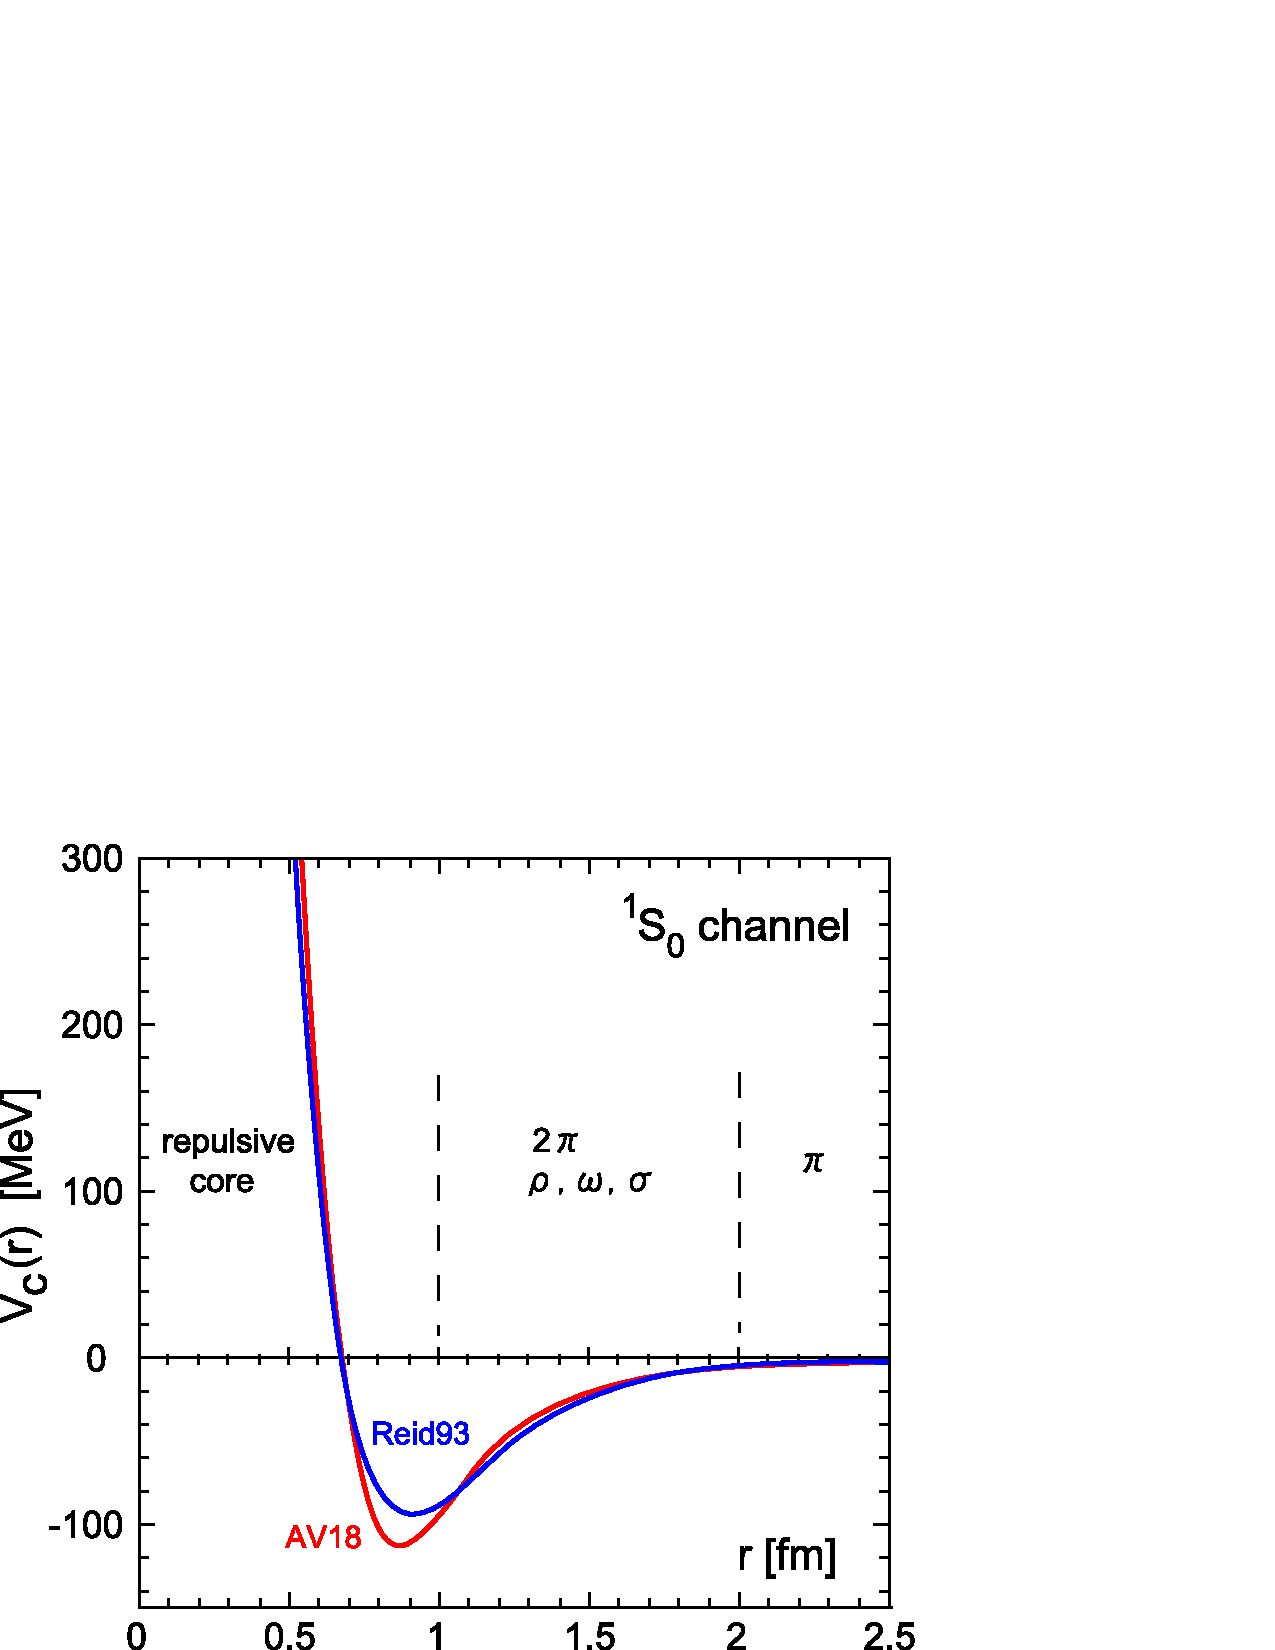
\includegraphics[width=0.8\columnwidth]{lattice1}\\[1ex]
\end{center}
}

\frame
{
  \frametitle{Brief summary of properties of the NN interaction}
\begin{small}
{\scriptsize
    \begin{enumerate}
\item Can use a one-boson exchange picture to construct a nucleon-nucleon
interaction a la QED
\item Non-relativistic approximation yields amongst other things a spin-orbit
force which is much stronger than in atoms.
\item At large intermediate distances pion exchange dominates while 
pion resonances (other mesons) dominate at intermediate and short range 
\item  Potentials are parameterized to fit selected two-nucleon data, binding energies and scattering phase shifts.
\item Nowaydays, chiral perturbation theory gives an effective theory that allows a systematic expansion in terms of contrallable parameters. Good basis for many-body physics
    \end{enumerate}
}
\end{small}
}






\section[Week 12]{Week 12}

\frame
{
  \frametitle{Topics for Week 12, March 17-21}
  \begin{block}{Nuclear shell model}
\begin{itemize}
\item Monday:
\item Short repetition from last week plus more on the particle-hole formalism
\item Configurations mixing and discussion of specific two-valence nucleon systems like $^{18}$O and $^{42}$Ca and other similar systems.
\item Wednesday:
\item Presentation of project 2 and discussion of necessary ingredients (continues next week as well)
\item No lecture on Friday.
\end{itemize}
The topics covered in this and next week's lectures can be found in Alex Brown's lecture notes, chapters 5, 18, 21-22.
See also Suhonen's chapter's 2 and 5.
  \end{block}
} 

\frame{
\frametitle{Slater determinants as basis states, Repetition}

The simplest possible choice for many-body wavefunctions are
\textit{product} wavefunctions.

\begin{small}
{\scriptsize
e.g., 
\[ 
\Psi(x_1, x_2, x_3, \ldots, x_A) \approx \phi_1(x_1) \phi_2(x_2) \phi_3(x_3) \ldots
\]
because we are really only good  at thinking about one particle at a time. Such 
product wavefunctions, without correlations (e.g. Jastrow-type functions), are easy to 
work with; for example, if the single-particle states $\{ \phi_i(x)\}$ are orthonormal, then 
the product wavefunctions are easy to orthonormalize.   

\medskip

Similarly, computing matrix elements of operators are relatively easy, because the 
integrals factorize.

\medskip

The price we pay is the lack of correlations, which we must build up by using many, many product 
wavefunctions. (Thus we have a trade-off: compact representation of correlations but 
difficult integrals versus easy integrals but many states required.) 

}\end{small}
}

\frame{
\frametitle{Slater determinants as basis states, repetition}

\begin{small}
{\scriptsize
Because we have fermions, we are required to have antisymmetric wavefunctions, e.g.
\[
\Psi(x_1, x_2, x_3, \ldots, x_A) = - \Psi(x_2, x_1, x_3, \ldots, x_A)
\]
etc. This is accomplished formally by using the determinantal formalism:
\[
\Psi(x_1, x_2, \ldots, x_N) 
= \frac{1}{\sqrt{N!}} 
\det \left | 
\begin{array}{cccc}
\phi_1(x_1) & \phi_1(x_2) & \ldots & \phi_1(x_N) \\
\phi_2(x_1) & \phi_2(x_2) & \ldots & \phi_2(x_N) \\
 \vdots & & &  \\
\phi_N(x_1) & \phi_N(x_2) & \ldots & \phi_N(x_N) 
\end{array}
\right |
\]
Product wavefunction + antisymmetry = Slater determinant. 

}\end{small}
}

\frame{
\frametitle{Slater determinants as basis states}

\begin{small}
{\scriptsize
\[
\Psi(x_1, x_2, \ldots, x_N) 
= \frac{1}{\sqrt{N!}} 
\det \left | 
\begin{array}{cccc}
\phi_1(x_1) & \phi_1(x_2) & \ldots & \phi_1(x_N) \\
\phi_2(x_1) & \phi_2(x_2) & \ldots & \phi_2(x_N) \\
 \vdots & & &  \\
\phi_N(x_1) & \phi_N(x_2) & \ldots & \phi_N(x_N) 
\end{array}
\right |
\]
Properties of the determinant (interchange of any two rows or 
any two columns yields a change in sign; thus no two rows and no 
two columns can be the same) lead to the Pauli principle:

\begin{itemize}

\item No two particles can be at the same place (two columns the same); and

\item No two particles can be in the same state (two rows the same).

\end{itemize}


}\end{small}
}

\frame{
\frametitle{Slater determinants as basis states}

\begin{small}
{\scriptsize
As a practical matter, however, Slater determinants beyond $N=4$ quickly become 
unwieldy. Thus we turn to the \textit{occupation representation} or 
\textit{second quantization} to simplify calculations. 

\bigskip

The occupation representation, using fermion \textit{creation} and \textit{annihilation} 
operators, is compact and efficient. It is also abstract and, at first encounter, not easy to 
internalize. It is inspired by other operator formalism, such as the ladder operators for 
the harmonic oscillator or for angular momentum, but unlike those cases, the operators 
\textit{do not have coordinate space representations}.

\bigskip

Instead, one can think of fermion creation/annihilation operators as a game of symbols that 
compactly reproduces what one would do, albeit clumsily, with full coordinate-space Slater 
determinants. 


}\end{small}
}


\frame{
\frametitle{Quick repetition of the occupation representation}

\begin{small}
{\scriptsize

We start with a set of orthonormal single-particle states $\{ \phi_i(x) \}$. 
(Note: this requirement, and others, can be relaxed, but leads to a 
more involved formalism.) \textit{Any} orthonormal set will do. 

\bigskip

To each single-particle state $\phi_i(x)$ we associate a creation operator 
$\hat{a}^\dagger_i$ and an annihilation operator $\hat{a}_i$. 

\bigskip

When acting on the vacuum state $| 0 \rangle$, the creation operator $\hat{a}^\dagger_i$ causes 
a particle to occupy the single-particle state $\phi_i(x)$:

\[
\phi_i(x) \rightarrow \hat{a}^\dagger_i |0 \rangle
\]

}\end{small}
}

\frame{
\frametitle{Quick repetition  of the occupation representation}

\begin{small}
{\scriptsize

But with multiple creation operators we can occupy multiple states:
\[
\phi_i(x) \phi_j(x^\prime) \phi_k(x^{\prime \prime}) 
\rightarrow \hat{a}^\dagger_i \hat{a}^\dagger_j \hat{a}^\dagger_k |0 \rangle.
\]

Now we impose antisymmetry, by having the fermion operators satisfy 
\textit{anticommutation relations}:
\[
\hat{a}^\dagger_i \hat{a}^\dagger_j + \hat{a}^\dagger_j \hat{a}^\dagger_i
= [ \hat{a}^\dagger_i ,\hat{a}^\dagger_j ]_+ 
= \{ \hat{a}^\dagger_i ,\hat{a}^\dagger_j \} = 0
\]
so that 
\[
\hat{a}^\dagger_i \hat{a}^\dagger_j = - \hat{a}^\dagger_j \hat{a}^\dagger_i
\]
Because of this property, automatically $\hat{a}^\dagger_i \hat{a}^\dagger_i = 0$, 
enforcing the Pauli exclusion principle.  Thus when writing a Slater determinant 
using creation operators, 
\[
\hat{a}^\dagger_i \hat{a}^\dagger_j \hat{a}^\dagger_k \ldots |0 \rangle
\]
each index $i,j,k, \ldots$ must be unique.

}\end{small}
}

% . . .  . . . . . . .   . .   . . ..  . .   . .   . . . . . . . ..  . . . . .


\frame{
\frametitle{Instant tour of the occupation representation}

\begin{small}

{\scriptsize
The annihilation operators also anticommute $\{ \hat{a}_i, \hat{a}_j \} = 0$ so that
\[
\hat{a}_i \hat{a}_j = - \hat{a}_j \hat{a}_i
\]
Furthermore, in case it is not obvious, the adjoint of a Slater determinant is 
\[
\left(\hat{a}^\dagger_i \hat{a}^\dagger_j \hat{a}^\dagger_k \ldots |0 \rangle\right)^\dagger
= \langle 0 | \ldots \hat{a}_k \hat{a}_j \hat{a}_i.
\]

We need two more rules. The first is that an annihilation operator 
$\hat{a}_i$ acting on a ket vacuum $| 0 \rangle$...\textit{annihilates} it entirely:
\[
\hat{a}_i | 0 \rangle = 0
\]
(also the adjoint: $\langle 0 | \hat{a}^\dagger  = 0$); 
\smallskip

furthermore the creation and annihilation operators with the same index $i$ have a 
special anticommutator:
\[
\{ \hat{a}_i , \hat{a}^\dagger_j \} = \delta_{ij}
\]
so that if $i,j$ are different the operators always anticommute.

}\end{small}
}
% . . .  . . . . . . .   . .   . . ..  . .   . .   . . . . . . . ..  . . . . .


\frame{
\frametitle{Slater determinants and the occupation representation}

\begin{small}

{\scriptsize
For computational work, we can go further and represent Slater determinants one of 
two ways:

\begin{itemize}

\item We can simply write down a list of occupied states, e.g. $ | 1,2 \rangle$
$ | 2,3 \rangle$, $| 4, 5 \rangle$, etc.; or

\item We can use bit notation: a one {\tt 1} for occupied and a zero {\tt 0} 
for unoccupied: $| 11000 \rangle$, $|01100 \rangle$, $| 00011 \rangle$ etc. 
\end{itemize}

Both have their advantages and disadvantages; for small number of particles the list of 
occupied states is more compact, but for large number of particles storing Slater determinants 
in bit form can be advantageous and is commonly used. This can form the topic for the final presentation for some of you.
}\end{small}
}

% . . .  . . . . . . .   . .   . . ..  . .   . .   . . . . . . . ..  . . . . .


\frame[containsverbatim]
{
  \frametitle{Configuration interaction (CI) theory}
\begin{small}
{\scriptsize
We have defined the ansatz for the ground state as 
\[
|\Phi_0\rangle = \left(\prod_{i=1}^n}\hat{a}_{i}^{\dagger}\right)|0\rangle,
\]
where the $i$ define different single-particle states up to the Fermi level. We have assumed that we have $n$ fermions. 
A given one-particle-one-hole ($1p1h$) state can be written as
\[
|\Phi_i^a\rangle = \hat{a}_{a}^{\dagger}\hat{a}_i|\Phi_0\rangle,
\]
while a $2p2h$ state can be written as
\[
|\Phi_{ij}^{ab}\rangle = \hat{a}_{a}^{\dagger}\hat{a}_{b}^{\dagger}\hat{a}_j\hat{a}_i|\Phi_0\rangle,
\]
and a general $npnh$ state as 
\[
|\Phi_{ijk\dots}^{abc\dots}\rangle = \hat{a}_{a}^{\dagger}\hat{a}_{b}^{\dagger}\hat{a}_{c}^{\dagger}\dots\hat{a}_k\hat{a}_j\hat{a}_i|\Phi_0\rangle.
\]
 }
 \end{small}
 }


\frame[containsverbatim]
{
  \frametitle{Configuration interaction (CI) theory}
\begin{small}
{\scriptsize
We can then expand our exact state function for the ground state 
as
\[
|\Psi_0\rangle=C_0|\Phi_0\rangle+\sum_{ai}C_i^a|\Phi_i^a\rangle+\sum_{abij}C_{ij}^{ab}|\Phi_{ij}^{ab}\rangle+\dots
=(C_0+\hat{C})|\Phi_0\rangle,
\]
where we have introduced the so-called correlation operator 
\[
\hat{C}=\sum_{ai}C_i^a\hat{a}_{a}^{\dagger}\hat{a}_i  +\sum_{abij}C_{ij}^{ab}\hat{a}_{a}^{\dagger}\hat{a}_{b}^{\dagger}\hat{a}_j\hat{a}_i+\dots
\]
Since the normalization of $\Psi_0$ is at our disposal and since $C_0$ is by hypothesis non-zero, we may arbitrarily set $C_0=1$ with 
corresponding proportional changes in all other coefficients. Using this so-called intermediate normalization we have
\[
\langle \Psi_0 | \Phi_0 \rangle = \langle \Phi_0 | \Phi_0 \rangle = 1, 
\]
resulting in 
\[
|\Psi_0\rangle=(1+\hat{C})|\Phi_0\rangle.
\]
 }
 \end{small}
 }


\frame[containsverbatim]
{
  \frametitle{Configuration interaction (CI) theory}
\begin{small}
{\scriptsize
We rewrite 
\[
|\Psi_0\rangle=C_0|\Phi_0\rangle+\sum_{ai}C_i^a|\Phi_i^a\rangle+\sum_{abij}C_{ij}^{ab}|\Phi_{ij}^{ab}\rangle+\dots,
\]
in a more compact form as 
\[
|\Psi_0\rangle=\sum_{PH}C_H^P\Phi_H^P=\left(\sum_{PH}C_H^P\hat{A}_H^P\right)|\Phi_0\rangle,
\]
where $H$ stands for $0,1,\dots,n$ hole states and $P$ for $0,1,\dots,n$ particle states. 
Our requirement of unit normalization gives
\[
\langle \Psi_0 | \Phi_0 \rangle = \sum_{PH}|C_H^P|^2= 1,
\]
and the energy can be written as 
\[
E= \langle \Psi_0 | \hat{H} |\Phi_0 \rangle= \sum_{PP'HH'}C_H^{*P}\langle \Phi_H^P | \hat{H} |\Phi_{H'}^{P'} \rangle C_{H'}^{P'}.
\]
 }
 \end{small}
 }


\frame[containsverbatim]
{
  \frametitle{Configuration interaction (CI) theory}
\begin{small}
{\scriptsize
Normally 
\[
E= \langle \Psi_0 | \hat{H} |\Phi_0 \rangle= \sum_{PP'HH'}C_H^{*P}\langle \Phi_H^P | \hat{H} |\Phi_{H'}^{P'} \rangle C_{H'}^{P'},
\]
is solved by diagonalization setting up the Hamiltonian matrix defined by the basis of all possible Slater determinants. A diagonalization
is equivalent to finding the variational minimum  of 
\[
 \langle \Psi_0 | \hat{H} |\Phi_0 \rangle-\lambda \langle \Psi_0 |\Phi_0 \rangle,
\]
where $\lambda$ is a variational multiplier to be identified with the energy of the system.
The minimization process results in 
\[
\delta\left[ \langle \Psi_0 | \hat{H} |\Phi_0 \rangle-\lambda \langle \Psi_0 |\Phi_0 \rangle\right]=
\sum_{P'H'}\left\{\delta[C_H^{*P}]\langle \Phi_H^P | \hat{H} |\Phi_{H'}^{P'} \rangle C_{H'}^{P'}+
C_H^{*P}\langle \Phi_H^P | \hat{H} |\Phi_{H'}^{P'} \rangle \delta[C_{H'}^{P'}]  .\right
\]
\[
.\left -
\lambda( \delta[C_H^{*P}]C_{H'}^{P'}+C_H^{*P}\delta[C_{H'}^{P'}]\right\} = 0.
\]
Since the coefficients $\delta[C_H^{*P}]$ and $\delta[C_{H'}^{P'}]$ are complex conjugates it is necessary and sufficient to require the quantities that multiply with $\delta[C_H^{*P}]$ to vanish.  
 }
 \end{small}
 }


\frame[containsverbatim]
{
  \frametitle{Configuration interaction (CI) theory}
\begin{small}
{\scriptsize
This leads to 
\[
\sum_{P'H'}\langle \Phi_H^P | \hat{H} |\Phi_{H'}^{P'} \rangle C_{H'}^{P'}-\lambda C_H^{P}=0,
\]
for all sets of $P$ and $H$.

If we then multiply by the corresponding $C_H^{*P}$ and sum over $PH$ we obtain
\[ 
\sum_{PP'HH'}C_H^{*P}\langle \Phi_H^P | \hat{H} |\Phi_{H'}^{P'} \rangle C_{H'}^{P'}-\lambda\sum_{PH}|C_H^P|^2=0,
\]
leading to the identification $\lambda = E$. This means that we have for all $PH$ sets
\begin{equation}
\sum_{P'H'}\langle \Phi_H^P | \hat{H} -E|\Phi_{H'}^{P'} \rangle = 0.\label{eq:fullci}
\end{equation}
 }
 \end{small}
 }


\frame[containsverbatim]
{
  \frametitle{Configuration interaction (CI) theory}
\begin{small}
{\scriptsize
An alternative way to derive the last equation is to start from 
\[
(\hat{H} -E)|\Psi_0\rangle = (\hat{H} -E)\sum_{P'H'}C_{H'}^{P'}|\Phi_{H'}^{P'} \rangle=0, 
\]
and if this equation is successively projected against all $\Phi_H^P$ in the expansion of $\Psi$, then the last equation on the previous slide
results.   As stated previously, one solves this equation normally by diagonalization. If we are able to solve this equation exactly (that is
numerically exactly) in a large Hilbert space (it will be truncated in terms of the number of single-particle states included in the definition
of Slater determinants), it can then serve as a benchmark for other many-body methods which approximate the correlation operator
$\hat{C}$.  

Let us then become more practical again.
 }
 \end{small}
 }



\frame{
\frametitle{Building a many-body basis}

\begin{small}

{\scriptsize

In project 2 the plan  is to construct a working code that constructs the 
many-body Hamiltonian matrix in a basis of Slater determinants and to find the low-lying eigenenergies. 
This is referred to as the configuration-interaction method or shell-model diagonalization 
(or the interacting shell model). 

\smallskip

The first step in such codes--and in your project--is to construct the many-body basis.  

\smallskip

While the formalism is independent of the choice of basis, the \textit{effectiveness} of a calculation 
will certainly be basis dependent. 

\smallskip

Furthermore there are common conventions useful to know.

}\end{small}
}

% . . .  . . . . . . .   . .   . . ..  . .   . .   . . . . . . . ..  . . . . .


\frame{
\frametitle{Building a many-body basis}

\begin{small}

{\scriptsize

First, the single-particle basis has angular momentum as a good quantum number.  You can 
imagine the single-particle wavefunctions being generated by a one-body Hamiltonian, 
for example a harmonic oscillator.  Modifications include harmonic oscillator plus 
spin-orbit splitting, or self-consistent mean-field potentials, or the Woods-Saxon potential which mocks 
up the self-consistent mean-field. 

\smallskip

For nuclei, the harmonic oscillator, modified by spin-orbit splitting, provides a useful language 
for describing single-particle states.

\smallskip

Each single-particle state is labeled by the following quantum numbers: 
\begin{itemize}
\item Orbital angular momentum $l$

\item Intrinsic spin $s$ = 1/2 for protons and neutrons

\item Angular momentum $j = l \pm 1/2$

\item $z$-component $j_z$ (or $m$)

\item Some labeling of the radial wavefunction, typically $n$ the number of nodes in 
the radial wavefunction, but in the case of harmonic oscillator one can also use 
the principal quantum number $N$, where the harmonic oscillator energy is $(N+3/2)\hbar \omega$. 

\end{itemize}

}\end{small}
}

% . . .  . . . . . . .   . .   . . ..  . .   . .   . . . . . . . ..  . . . . .


\frame{
\frametitle{Building a many-body basis}

\begin{small}

{\scriptsize

In this format one labels states by $n(l)_j$, with $(l)$ replaced by a letter:
$s$ for $l=0$, $p$ for $l=1$, $d$ for $l=2$, $f$ for $l=3$, and thenceforth alphabetical.

\vspace{-2cm}
 \begin{center}
 \includegraphics[scale=0.30,clip]{sps}
 \end{center}

}\end{small}
}

% . . .  . . . . . . .   . .   . . ..  . .   . .   . . . . . . . ..  . . . . .


\frame{
\frametitle{Building a many-body basis}

\begin{small}

{\scriptsize
 In practice the single-particle space has to be severely truncated.  This truncation is 
typically based upon the \textit{single-particle energies}, which is the effective energy 
from a mean-field potential. 

\smallskip

Sometimes we freeze the core and only consider a valence space. For example, one 
may assume a frozen $^{4}$He core, with 2 protons and 2 neutrons in the $0s_{1/2}$ 
shell, and then only allow active particles in the $0p_{1/2}$ and $0p_{3/2}$ orbits. 

\smallskip

Another example is a frozen $^{16}$O core, with 8 protons and 8 neutrons filling the 
$0s_{1/2}$,  $0p_{1/2}$ and $0p_{3/2}$ orbits, with valence particles in the 
$0d_{5/2}, 1s_{1/2}$ and $0d_{3/2}$ orbits.

\smallskip

Sometimes we refer to nuclei by the valence space where their last nucleons go.  
So, for example, we call $^{12}$C a $p$-shell nucleus, while $^{26}$Al is an 
$sd$-shell nucleus and $^{56}$Fe is a $pf$-shell nucleus.

}\end{small}
}

% . . .  . . . . . . .   . .   . . ..  . .   . .   . . . . . . . ..  . . . . .


\frame{
\frametitle{Building a many-body basis}

There are different kinds of truncations.

\smallskip
\begin{small}

{\scriptsize

For example, one can start with `filled' orbits (almost always the lowest), and then 
allow one, two, three... particles excited out of those filled orbits. These are called 
1p-1h, 2p-2h, 3p-3h excitations. 
\vspace{-2cm}
 \begin{center}
 \includegraphics[scale=0.30,clip]{filled}
 \end{center}


}\end{small}
}


% . . .  . . . . . . .   . .   . . ..  . .   . .   . . . . . . . ..  . . . . .


\frame{
\frametitle{Building a many-body basis}

There are different kinds of truncations.

\smallskip
\begin{small}

{\scriptsize

For example, one can start with `filled' orbits (almost always the lowest), and then 
allow one, two, three... particles excited out of those filled orbits. These are called 
1p-1h, 2p-2h, 3p-3h excitations. 
\vspace{-2cm}
 \begin{center}
 \includegraphics[scale=0.30,clip]{ph}
 \end{center}


}\end{small}
}
% . . .  . . . . . . .   . .   . . ..  . .   . .   . . . . . . . ..  . . . . .


% . . .  . . . . . . .   . .   . . ..  . .   . .   . . . . . . . ..  . . . . .


\frame{
\frametitle{Building a many-body basis}

There are different kinds of truncations.

\smallskip
\begin{small}

{\scriptsize

Alternately, one can state a maximal orbit and allow all possible configurations with 
particles occupying states up to that maximum. This is called \textit{full configuration}.
\vspace{-2cm}
 \begin{center}
 \includegraphics[scale=0.30,clip]{fc}
 \end{center}


}\end{small}
}


% . . .  . . . . . . .   . .   . . ..  . .   . .   . . . . . . . ..  . . . . .


\frame{
\frametitle{Building a many-body basis}

There are different kinds of truncations.

\smallskip
\begin{small}

{\scriptsize

Finally, for particular use in nuclear physics, there is the \textit{energy} truncation, also 
called the $N\hbar\Omega$ or $N_{max}$ truncation. 

\smallskip
 Here one works in a harmonic oscillator basis, with each major oscillator shell assigned 
a principal quantum number $N=0,1,2,3,...$. 
\vspace{-2cm}
 \begin{center}
 \includegraphics[scale=0.30,clip]{ho}
 \end{center}


}\end{small}
}
% . . .  . . . . . . .   . .   . . ..  . .   . .   . . . . . . . ..  . . . . .


\frame{
\frametitle{Building a many-body basis}

The $N\hbar\Omega$ or $N_{max}$ truncation:
\smallskip
\begin{small}

{\scriptsize

Any configuration is given an noninteracting energy, which is the sum 
of the single-particle harmonic oscillator energies. (Thus this ignores 
spin-orbit splitting.)
%\vspace{-1cm}
 \begin{center}
 \includegraphics[scale=0.20,clip]{N0}
 \end{center}


}\end{small}


}
% . . .  . . . . . . .   . .   . . ..  . .   . .   . . . . . . . ..  . . . . .


\frame{
\frametitle{Building a many-body basis}

The $N\hbar\Omega$ or $N_{max}$ truncation:
\smallskip
\begin{small}

{\scriptsize

Excited state are labeled relative to the lowest configuration by the 
number of harmonic oscillator quanta
\vspace{-2cm}
 \begin{center}
 \includegraphics[scale=0.20,clip]{N2}
 \end{center}
A case of $N=2$.

}\end{small}


}
% . . .  . . . . . . .   . .   . . ..  . .   . .   . . . . . . . ..  . . . . .


\frame{
\frametitle{Building a many-body basis}

The $N\hbar\Omega$ or $N_{max}$ truncation:
\smallskip
\begin{small}

{\scriptsize

Excited state are labeled relative to the lowest configuration by the 
number of harmonic oscillator quanta
\vspace{-2cm}
 \begin{center}
 \includegraphics[scale=0.20,clip]{N2b}
 \end{center}
Another case of $N=2$.

\bigskip

This truncation is useful because: if one includes \textit{all} configuration up to 
some $N_{max}$, and has a translationally invariant interaction, then the intrinsic 
motion and the center-of-mass motion factor. In other words, we can know exactly 
the center-of-mass wavefunction. 
}\end{small}


}
% . . .  . . . . . . .   . .   . . ..  . .   . .   . . . . . . . ..  . . . . .

\frame{
\frametitle{Building a many-body basis}

\begin{small}

{\scriptsize
In almost all cases, the many-body Hamiltonian is rotationally invariant. This means 
it commutes with the operators $\hat{J}^2, \hat{J}_z$ and so eigenstates will have 
good $J,M$. Furthermore, the eigenenergies do not depend upon the orientation $M$. 

\bigskip

Therefore we can choose to construct a many-body basis which has fixed $M$; this is 
called an $M$-scheme basis. 

\smallskip

Alternately, one can construct a many-body basis which has fixed $J$, or a $J$-scheme 
basis. 

\smallskip

The Hamiltonian matrix will have smaller dimensions (a factor of 10 or more)
 in the $J$-scheme than in the $M$-scheme. 
On the other hand, as we'll show in the next slide, the $M$-scheme is very easy to 
construct with Slater determinants, while the $J$-scheme basis states, and thus the 
matrix elements, are more complicated, almost always being linear combinations of 
$M$-scheme states. $J$-scheme bases are important and useful, but we'll focus on the 
simpler $M$-scheme.

}\end{small}
}


% . . .  . . . . . . .   . .   . . ..  . .   . .   . . . . . . . ..  . . . . .


\frame{
\frametitle{Building a many-body basis}

\begin{small}

{\scriptsize

The quantum number $m$ is additive (because the underlying group is Abelian): 
if a Slater determinant $\hat{a}_i^\dagger \hat{a}^\dagger_j \hat{a}^\dagger_k \ldots 
| 0 \rangle$ is built from single-particle states all with good $m$, then 
the total 
\[
M = m_i + m_j + m_k + \ldots
\]
This is \textit{not} true of $J$, because the angular momentum group SU(2) is not Abelian.

\bigskip

The upshot is that 
\begin{itemize}

\item It is easy to construct a Slater determinant with good total $M$;

\item It is trivial to calculate $M$ for each Slater determinant;

\item So it is easy to construct an $M$-scheme basis with fixed total $M$.

\end{itemize}

Note that the individual $M$-scheme basis states will \textit{not}, in general, 
have good total $J$. 
Because the Hamiltonian is rotationally invariant, however, the eigenstates will 
have good $J$. (The situation is muddied when one has states of different $J$ that are 
nonetheless degenerate.) 

}\end{small}
}

% . . .  . . . . . . .   . .   . . ..  . .   . .   . . . . . . . ..  . . . . .


\frame{
\frametitle{Building a many-body basis}

\begin{small}

{\scriptsize

Example: two $j=1/2$ orbits:
\begin{center}

\begin{tabular}{|c|c|c|c|c|} \hline
Index & $n$ & $l$  & $j$ & $m$ \\ \hline 
1 & 0 & 0 & 1/2 & -1/2 \\
2 & 0 & 0 & 1/2 &  1/2 \\
3 & 1 & 0 & 1/2 & -1/2 \\
4 & 1 & 0 & 1/2 & 1/2 \\ \hline
\end{tabular}
%
Note: the order is arbitrary
\end{center}
There are $\left ( \begin{array}{c} 4 \\ 2 \end{array} \right) = 6$ two-particle states, 
which we list with the total $M$:

\begin{center}
\begin{tabular}{|c|c|}\hline
Occupied & $M$  \\ \hline
1,2 & 0    \\
1,3 & -1              \\
1,4 & 0             \\
2,3 & 0           \\
2,4 & 1 \\
3,4 &  0     \\ \hline
\end{tabular}
There are 4 states with $M= 0$, 
and 1 each with $M = \pm 1$.
\end{center}


}\end{small}
}
% . . .  . . . . . . .   . .   . . ..  . .   . .   . . . . . . . ..  . . . . .


\frame{
\frametitle{Building a many-body basis}

\begin{small}

{\scriptsize

Example: consider using only single particle states from the $0d_{5/2}$ space. 
They have the following quantum numbers

\begin{center}

\begin{tabular}{|c|c|c|c|c|} \hline
Index & $n$ & $l$  & $j$ & $m$ \\ \hline 
1 & 0 & 2 & 5/2 & -5/2 \\
2 & 0 & 2 & 5/2 & -3/2 \\
3 & 0 & 2 & 5/2 & -1/2 \\
4 & 0 & 2 & 5/2 & 1/2 \\
5 & 0 & 2 & 5/2 & 3/2 \\
6 & 0 & 2 & 5/2 &  5/2 \\ \hline
\end{tabular}
%
\end{center}
There are $\left ( \begin{array}{c} 6 \\ 2 \end{array} \right) = 15$ two-particle states, 
which we list with the total $M$:

\begin{center}
\begin{tabular}{|c|c||c|c||c|c|}\hline
Occupied & $M$ & Occupied & $M$ &Occupied & $M$ \\ \hline
1,2 & -4   &  2,3 & -2  &  3,5 & 1 \\
1,3 & -3  &  2,4 & -1 &    3,6 & 2             \\
1,4 & -2  &  2,5 & 0 &     4,5 & 2            \\
1,5 & -1  &  2,6 & 1 &     4,6 & 3          \\
1,6 & 0  &  3,4 & 0 &      5,6 & 4         \\ \hline
\end{tabular}

\end{center}
There are 3 states with $M= 0$, 2 with $M = 1$, and so on.


}\end{small}
}


\section[Week 13]{Week 13}

\frame
{
  \frametitle{Topics for Week 13, March 24-28}
  \begin{block}{Nuclear shell model}
\begin{itemize}
\item Monday:
\item Repetion from last week and discussion of project 2.
\item Wednesday:
\item Angular momentun couplings, Wigner-Eckart theorem and computation of two-body matrix elemen
\item Possibly also discussion of project 2
\item Friday:
\item More on angular momentum, the Wigner-Eckart theorem and computation of two-body matrix elements
\item Discussion of project 2.
\item Summary of shell-model studies and if time short prelude to Alex Brown's suite of nuclear structure  codes. 
\end{itemize}
The topics covered in this week's lectures can be found in Alex Brown's lecture notes, chapters 5, 18.

  \end{block}
} 



\frame{
\frametitle{Project 2}

The basic goal of project 2 is for you to build your own configuration-interaction  shell-model 
code. The code will be fairly basic; it will assume that we have 
a single species of particles, e.g. only neutrons, 
and you could, if you wish to,  read in uncoupled two-body matrix elements.  Furthermore the pieces of the code will not 
be the most efficient.  Nonetheless it will be usable; most importantly, you will gain a good idea of what goes into a many-body shell-model code.

}


% . . .  . . . . . . .   . .   . . ..  . .   . .   . . . . . . . ..  . . . . .
\frame{
\frametitle{Project 2, step 1}

\begin{small}
{\scriptsize

The first step  is to construct the $M$-scheme basis of Slater determinants.
Here $M$-scheme means the total $J_z$ of the many-body states is fixed.

The steps could be:

\begin{itemize}

\item  Read in a user-supplied file of single-particle states (examples can be given) or just code these internally;

\item Ask for the total $M$ of the system and the number of particles $N$;

\item Construct all the $N$-particle states with given $M$.  You will validate the code by 
comparing both the number of states and specific states.

\end{itemize}
}
\end{small}
}



% . . .  . . . . . . .   . .   . . ..  . .   . .   . . . . . . . ..  . . . . .
\frame[containsverbatim]{
\frametitle{Project 2, step 1}

\begin{small}
{\scriptsize

The format of a possible input  file could be

\begin{verbatim}
12         ! number of single-particle states
1     1     0      1     -1      !   index   nrnodes   l    2 x j      2 x jz
2     1     0      1      1
3     0     2      3     -3
4     0     2      3     -1
5     0     2      3      1
6     0     2      3      3
7     0     2      5     -5
8     0     2      5     -3
9     0     2      5     -1
10    0     2      5      1
11    0     2      5      3
12    0     2      5      5
\end{verbatim}

This represents the $1s_{1/2}$-$0d_{3/2}$-$0d_{5/2}$ valence space, or the $sd$-space.  There are 
twelve single-particle states, labeled by an overall index, and which have associated quantum 
numbers the number of radial nodes, the orbital angular momentum $l$, and the 
angular momentum $j$ and third component $j_z$.  To keep everything as integers, we could store $2 \times j$ and 
$2 \times j_z$. 

}
\end{small}
}
% . . .  . . . . . . .   . .   . . ..  . .   . .   . . . . . . . ..  . . . . .

% . . .  . . . . . . .   . .   . . ..  . .   . .   . . . . . . . ..  . . . . .
\frame{
\frametitle{Project 2, step 1}


To read in the single-particle states you need to:
\medskip

\begin{itemize}


\item Open the file 

\item  Read the number of single-particle states (in the above example, 12);  allocate memory; all you need is a single array storing $2\times j_z$ for each state, labeled by 
the index;

\item Read in the quantum numbers and store $2 \times j_z$ (and anything else you happen to want).

\end{itemize}

}

\frame{
\frametitle{Project 2, step 1}



The next step is to read in the number of particles $N$ and the fixed total $M$ (or, actually, $2 \times M$). 
For this project we assume only a single species of particles, say neutrons, although this can be 
relaxed. \textit{Note}: Although it is often a good idea to try to write a more general code, given the 
short time alloted we would suggest you keep your ambition in check, at least in the initial phases of the 
project.  

\bigskip

You should probably write an error trap to make sure $N$ and $M$ are congruent; if $N$ is even, then 
$2 \times M$ should be even, and if $N$ is odd then $2\times M$ should be odd. 

}

% . . .  . . . . . . .   . .   . . ..  . .   . .   . . . . . . . ..  . . . . .
\frame{
\frametitle{Project 2, step 1}

The final step is to generate the set of $N$-particle Slater determinants with fixed $M$. 
The Slater determinants will be stored in occupation representation.  Although in many codes
this representation is done compactly in bit notation ({\tt 1}s and {\tt 0}s), but for 
greater transparency and simplicity we will list the occupied single particle states.
 Hence we can 
store the Slater determinant basis states as 

\smallskip
{\tt sd(i,j)}

\smallskip

an array of dimension $N_{SD}$, the number of Slater determinants, by $N$, the number of occupied 
state. So if for the 7th Slater determinant the 2nd, 3rd, and 9th single-particle states are occupied, 
then {\tt sd(7,1)} = 2, {\tt sd(7,2)} = 3, and {\tt sd(7,3)} = 9.

}

% . . .  . . . . . . .   . .   . . ..  . .   . .   . . . . . . . ..  . . . . .
\frame{
\frametitle{Project 2, step 1}

\begin{small}
{\scriptsize
We can construct an occupation representation of Slater determinants by the \textit{odometer}
method.  Consider $N_{sp} = 12$ and $N=4$. 
Start with the first 4 states occupied, that is:

\smallskip

\noindent {\tt sd(1,:)= 1,2,3,4} (also written as $|1,2,3,4 \rangle$

\smallskip

Now increase the last occupance recursively:

\smallskip

\noindent {\tt sd(2,:)= 1,2,3,5}

\noindent {\tt sd(3,:)= 1,2,3,6}

\noindent {\tt sd(4,:)= 1,2,3,7}


$\ldots$

\noindent {\tt sd(9,:)= 1,2,3,12}

\smallskip

Then start over with 

\smallskip

\noindent {\tt sd(10,:)= 1,2,4,5}


\smallskip

and again increase the rightmost digit

\noindent {\tt sd(11,:)= 1,2,4,6}

\noindent {\tt sd(12,:)= 1,2,4,7}

$\ldots$

\noindent {\tt sd(17,:)= 1,2,4,12}

\smallskip

}\end{small}

}
% . . .  . . . . . . .   . .   . . ..  . .   . .   . . . . . . . ..  . . . . .
% . . .  . . . . . . .   . .   . . ..  . .   . .   . . . . . . . ..  . . . . .
\frame{
\frametitle{Project 2, step 1}
When we restrict ourselves to an $M$-scheme basis, we could choose two paths. 
The first is simplest (and simplest is often best, at 
least in the first draft of a code): generate \textit{all} possible Slater determinants, 
and then extract from this initial list a list of those Slater determinants with a given 
$M$. (You will need to write a short function or routine that computes $M$ for any 
given occupation.)  

\smallskip

Alternately, and not too difficult, is to run the odometer routine twice: each time, as 
as a Slater determinant is calculated, compute $M$, but do not store the Slater determinants 
except the current one. You can then count up the number of Slater determinants with a 
chosen $M$.  Then allocated storage for the Slater determinants, and run the odometer 
algorithm again, this time storing Slater determinants with the desired $M$ (this can be 
done with a simple logical flag). 

}

% . . .  . . . . . . .   . .   . . ..  . .   . .   . . . . . . . ..  . . . . .
\frame[containsverbatim]{
\frametitle{Project 2, step 1}


\begin{small}
{\scriptsize

\textit{Some example solutions}:  Let's begin with a simple case, the $0d_{5/2}$ space:
\begin{verbatim}
6         ! number of single-particle states
1     0     2      5     -5
2     0     2      5     -3
3     0     2      5     -1
4     0     2      5      1
5     0     2      5      3
6     0     2      5      5
\end{verbatim}
For two particles, there are a total of 15 states, which we list here with the total $M$:
\medskip

\noindent $| 1,2 \rangle$, $M= -4$; 
 $| 1,3 \rangle$, $M= -3$

\noindent  $| 1,4 \rangle$, $M= -2$; 
 $| 1,5 \rangle$, $M= -1$

\noindent $| 1,5 \rangle$, $M= 0$; 
 $| 2,3 \rangle$, $M= -2$

\noindent $| 2,4 \rangle$, $M= -1$;
 $| 2,5 \rangle$, $M= 0$

\noindent $| 2,6 \rangle$, $M= 1$;
 $| 3,4 \rangle$, $M= 0$

\noindent $| 3,5 \rangle$, $M= 1$;
 $| 3,6 \rangle$, $M= 2$

\noindent $| 4,5 \rangle$, $M= 2$;
 $ | 4,6 \rangle$, $M= 3$

\noindent $| 5,6 \rangle$, $M= 4$

Of these, there are only 3 states with $M=0$. 
}\end{small}

}

% . . .  . . . . . . .   . .   . . ..  . .   . .   . . . . . . . ..  . . . . .
\frame{
\frametitle{Project 2, step 1}

\textit{You should try} by hand to show that in this same single-particle space, that for 
$N=3$ there are 3 states with $M=1/2$ and for $N= 4$ there are also only 3 states with $M=0$. 

\textit{To test your code}, confirm the above. 

\bigskip

Also, 
for the $sd$-space given above, for $N=2$ there are 14 states with $M=0$, for $N=3$ there are 37 
states with $M=1/2$, for $N=4$ there are 81 states with $M=0$.

}


% . . .  . . . . . . .   . .   . . ..  . .   . .   . . . . . . . ..  . . . . .
\frame[containsverbatim]{
\frametitle{Project 2, step 1}
For our project, we will only consider the pairing model.
A simple space is the $(1/2)^2$ space
\begin{verbatim}
4         ! number of single-particle states
1     0     0      1     -1
2     0     0      1      1
3     1     0      1     -1
4     1     0      1      1
\end{verbatim}
For $N=2$ there are 4 states with $M=0$; show this by hand and confirm your code reproduces it. 

}

% . . .  . . . . . . .   . .   . . ..  . .   . .   . . . . . . . ..  . . . . .
\frame[containsverbatim]{
\frametitle{Project 2, step 1}


Another, slightly more challenging space is the $(1/2)^4$ space, that is, 
\begin{verbatim}
8         ! number of single-particle states
1     0     0      1     -1
2     0     0      1      1
3     1     0      1     -1
4     1     0      1      1
5     2     0      1     -1
6     2     0      1      1
7     3     0      1     -1
8     3     0      1      1
\end{verbatim}

For $N=2$ there are 16 states with $M=0$; for $N=3$ there are 24 states with $M=1/2$, and for 
$N=4$ there are 36 states with $M=0$. 

}

% . . .  . . . . . . .   . .   . . ..  . .   . .   . . . . . . . ..  . . . . .
\frame{
\frametitle{Project 2, step 1}
\begin{small}
{\scriptsize 

In the shell-model context we can interpret this as 4 $s_{1/2}$ levels, with $m = \pm 1/2$, we can also think of these are simple 4 pairs,  $\pm k, k = 1,2,3,4$. Later on we will 
assign single-particle energies,  depending on the radial quantum number $n$, that is, 
$\epsilon_k = |k| \delta$ so that they are equally spaced.
}
\end{small}

}

% . . .  . . . . . . .   . .   . . ..  . .   . .   . . . . . . . ..  . . . . .
\frame{
\frametitle{Project 2, step 1}
\begin{small}
{\scriptsize 
For application in the pairing model we can go further and consider only states with 
no ``broken pairs,'' that is, if $+k$ is filled (or $m = +1/2$, so is $-k$ ($m=-1/2$). 
If you want, you can write your code to accept only these, and obtain the following 
6 states:

$|           1,           2 ,          3         ,       4  \rangle , $

$|            1      ,     2        ,        5         ,       6 \rangle , $

$|            1         ,       2     ,           7         ,       8  \rangle , $

$|            3        ,        4      ,          5          ,      6  \rangle , $

$|            3        ,        4      ,          7         ,       8  \rangle , $

$|            5        ,        6     ,           7     ,           8  \rangle $
}
\end{small}

}
% . . .  . . . . . . .   . .   . . ..  . .   . .   . . . . . . . ..  . . . . .
\frame{
\frametitle{Project 2, step 1}

Hints for coding

\begin{itemize}

\item Write small modules (routines/functions) ; avoid big functions 
that do everything. (But not too small.)

\item Write lots of error traps, even for things that are `obvious.'

\item Document as you go along.  For each function write
a header that includes: (A) Main purpose of function; (B) names and 
brief explanation of input 
variables, if any; (C) names and brief explanation of output variables, 
if any; (D) functions called by this function; (E)
called by which functions

\end{itemize}

}
% . . .  . . . . . . .   . .   . . ..  . .   . .   . . . . . . . ..  . . . . .
\frame{
\frametitle{Project 2, step 1}

Hints for coding

\begin{itemize}

\item When debugging, print out intermediate values. It's almost impossible to debug a 
code by looking at it--the code will almost always win a `staring contest.'

\item Validate code with SIMPLE CASES. Validate early and often.   

\end{itemize}

The number one mistake is using a too complex a system to test. \textit{For example} 
If you are computing particles in a potential in a box, try removing the potential--you should get 
particles in a box. And start with one particle, then two, then three... Don't start with 
eight particles.
}
% . . .  . . . . . . .   . .   . . ..  . .   . .   . . . . . . . ..  . . . . .
\frame{
\frametitle{Bit representation}

Our recommended occupation representation, e.g. $| 1,2,4,8 \rangle$, is 
easy to code, but numerically inefficient when one has hundreds of 
millions of Slater determinants.

\medskip

In state-of-the-art shell-model codes, one generally uses \textit{bit 
representation}, i.e. $|1101000100... \rangle$ where one stores 
the Slater determinant as a single (or a small number of) integer.

\medskip

This is much more compact, but more intricate to code with considerable 
more overhead. There exist 
bit-manipulation functions. 
This is left as a challenge for those of you who would like to study this topic further for the final project.

}


\frame{
\frametitle{Example case: pairing Hamiltonian}

\begin{small}
{\scriptsize
We consider a space with $2\Omega$ single-particle states, with each 
state labeled by 
$k = 1, 2, 3, \Omega$ and $m = \pm 1/2$. The convention is that 
the state with $k>0$ has $m = + 1/2$ while $-k$ has $m = -1/2$.

\smallskip

The Hamiltonian we consider is 
\[
\hat{H} = -G \hat{P}_+ \hat{P}_-,
\]
where
\[
\hat{P}_+ = \sum_{k > 0} \hat{a}^\dagger_k \hat{a}^\dagger_{-{k}}.
\]
and $\hat{P}_- = ( \hat{P}_+)^\dagger$.

\bigskip

We will first solve this using a trick, the quasi-spin formalism, to obtain the 
exact results. Then we will try again using the explicit Slater determinant formalism.


}\end{small}

}


% . . .  . . . . . . .   . .   . . ..  . .   . .   . . . . . . . ..  . . . . .
\frame{
\frametitle{Example case: pairing Hamiltonian}

\begin{small}
{\scriptsize
One can show (and this is part of the project) that
\[
\left [ \hat{P}_+, \hat{P}_- \right ] = \sum_{k> 0} \left( \hat{a}^\dagger_k \hat{a}_k 
+ \hat{a}^\dagger_{-{k}} \hat{a}_{-{k}} - 1 \right) = \hat{N} - \Omega.
\]
Now define 
\[
\hat{P}_z = \frac{1}{2} ( \hat{N} -\Omega).
\]
Finally you can show
\[
\left [ \hat{P}_z , \hat{P}_\pm \right ] = \pm \hat{P}_\pm.
\]
This means the operators $\hat{P}_\pm, \hat{P}_z$ form an SU(2) algebra, and we can 
all our insights about angular momentum, even though there is no actual 
angular momentum involved (this is similar to project 1).

\smallskip
So we rewrite the Hamiltonian to make this explicit:
\[
\hat{H} = -G \hat{P}_+ \hat{P}_- 
= -G \left( \hat{P}^2 - \hat{P}_z^2 + \hat{P}_z\right)
\]

}\end{small}

}

% . . .  . . . . . . .   . .   . . ..  . .   . .   . . . . . . . ..  . . . . .
\frame{
\frametitle{Example case: pairing Hamiltonian}

\begin{small}
{\scriptsize
Because of the SU(2) algebra, we \textit{know} that the eigenvalues of 
$\hat{P}^2$ must be of the form $p(p+1)$, with $p$ either integer or half-integer, and the eigenvalues of $\hat{P}_z$ 
are $m_p$ with $p \geq | m_p|$, with $m_p$ also integer or half-integer. 

\bigskip

But because $\hat{P}_z = (1/2)(\hat{N}-\Omega)$, we know that for $N$ particles 
the value $m_p = (N-\Omega)/2$. Furthermore, the values of $m_p$ range from 
$-\Omega/2$ (for $N=0$) to $+\Omega/2$ (for $N=2\Omega$, with all states filled). 

\smallskip

We deduce the maximal $p = \Omega/2$ and for a given $n$ the 
values range of $p$ range from $|N-\Omega|/2$ to $\Omega/2$ in steps of 1 
(for an even number of particles) 

\smallskip

Following Racah we introduce the notation
$p = (\Omega - v)/2$
where $v = 0, 2, 4,..., \Omega - |N-\Omega|$ 
With this it is easy to deduce that the eigenvalues of the pairing Hamiltonian are
\[
-G(N-v)(2\Omega +2-N-v)/4
\]
This also works for $N$ odd, with $v= 1,3,5, \dots$.


}\end{small}

}

% . . .  . . . . . . .   . .   . . ..  . .   . .   . . . . . . . ..  . . . . .
\frame{
\frametitle{Example case: pairing Hamiltonian}

\begin{small}
{\scriptsize
Let's take a specific example: $\Omega = 3$ so there are 6 single-particle states, 
and $N = 3$, with $v= 1,3$. Therefore there are two distinct eigenvalues, 
\[
E = -2G, 0
\]
Now let's work this out explicitly. The single particle space we write as 
\begin{center}
\begin{tabular}{|c| c| c|} \hline
Index & $k$ & $m$ \\ \hline
1 & 1 & -1/2 \\
2 & -1 & 1/2 \\
3 & 2 & -1/2 \\
4 & -2 & 1/2 \\
5 & 3 & -1/2 \\
6 & -3 & 1/2 \\ \hline
\end{tabular}
\end{center}


 There are  $\left( 
\begin{array}{c}6 \\ 3 \end{array} \right) = 20$ three-particle states, but there 
are 9 states with $M = +1/2$:

 $| 1,2,3 \rangle, |1,2,5\rangle, | 1,4,6 \rangle, | 2,3,4 \rangle, |2,3,6 \rangle, 
| 2,4,5 \rangle, | 2, 5, 6 \rangle, |3,4,6 \rangle, | 4,5,6 \rangle$.

}\end{small}

}

% . . .  . . . . . . .   . .   . . ..  . .   . .   . . . . . . . ..  . . . . .
\frame{
\frametitle{Example case: pairing Hamiltonian }

\begin{small}
{\scriptsize

In this basis, the operator 
\[
\hat{P}_+
= \hat{a}^\dagger_1 \hat{a}^\dagger_2 + \hat{a}^\dagger_3 \hat{a}^\dagger_4 +
\hat{a}^\dagger_5 \hat{a}^\dagger_6 
\]
From this we can determine that 
\[
\hat{P}_- | 1, 4, 6 \rangle = \hat{P}_- | 2, 3, 6 \rangle
= \hat{P}_- | 2, 4, 5 \rangle = 0
\]
so those states all have eigenvalue 0.
}
\end{small}


}

% . . .  . . . . . . .   . .   . . ..  . .   . .   . . . . . . . ..  . . . . .
\frame{
\frametitle{Example case: pairing Hamiltonian }


\begin{small}
{\scriptsize

Now for further example, 

\[
\hat{P}_- | 1,2,3 \rangle = | 3 \rangle
\]
so
\[
\hat{P}_+ \hat{P}_- | 1,2,3\rangle = | 1,2,3\rangle+ | 3,4,3\rangle + | 5,6,3\rangle
\]
The second term vanishes because state 3 is occupied twice, and reordering the last 
term we
get
\[
\hat{P}_+ \hat{P}_- | 1,2,3\rangle = | 1,2,3\rangle+ |3, 5,6\rangle
\]
without picking up a phase.

 
}
\end{small}

}

% . . .  . . . . . . .   . .   . . ..  . .   . .   . . . . . . . ..  . . . . .
\frame{
\frametitle{Example case: pairing Hamiltonian }


\begin{small}
{\scriptsize

Continuing in this fashion, with the previous ordering of the many-body states
(  $| 1,2,3 \rangle, |1,2,5\rangle, | 1,4,6 \rangle, | 2,3,4 \rangle, |2,3,6 \rangle, 
| 2,4,5 \rangle, | 2, 5, 6 \rangle, |3,4,6 \rangle, | 4,5,6 \rangle$) the 
Hamiltonian matrix of this system is 
\[
H = -G\left( 
\begin{array}{ccccccccc}
1 & 0 & 0 & 0 & 0 & 0 & 0 & 0 & 1  \\
0 & 1 & 0 & 0 & 0 & 0 & 0 & 1 & 0  \\
0 & 0 & 0 & 0 & 0 & 0 & 0 & 0 & 0  \\
0 & 0 & 0 & 1 & 0 & 0 & 1 & 0 & 0  \\
0 & 0 & 0 & 0 & 0 & 0 & 0 & 0 & 0  \\
0 & 0 & 0 & 0 & 0 & 0 & 0 & 0 & 0  \\
0 & 0 & 0 & 1 & 0 & 0 & 1 & 0 & 0  \\
0 & 0 & 0 & 0 & 0 & 0 & 0 & 0 & 0  \\
0 & 1 & 0 & 0 & 0 & 0 & 0 & 1 & 0  \\
1 & 0 & 0 & 0 & 0 & 0 & 0 & 0 & 1  
\end{array} \right )
\] 
This is useful for our project.  One can by hand confirm 
that there are 3 eigenvalues $-2G$ and 6 with value zero.

}
\end{small}

}


% . . .  . . . . . . .   . .   . . ..  . .   . .   . . . . . . . ..  . . . . .
\frame[containsverbatim]{
\frametitle{Example case: pairing Hamiltonian }

Another example

\begin{small}
{\scriptsize

Using the $(1/2)^4$ single-particle space
\begin{verbatim}
8         ! number of single-particle states
1     0     0      1     -1
2     0     0      1      1
3     1     0      1     -1
4     1     0      1      1
5     2     0      1     -1
6     2     0      1      1
7     3     0      1     -1
8     3     0      1      1
\end{verbatim}
and then taking only 4-particle, $M=0$ states that have no `broken pairs', there are six basis Slater 
determinants:

$|           1,           2 ,          3         ,       4  \rangle , $

$|            1      ,     2        ,        5         ,       6 \rangle , $

$|            1         ,       2     ,           7         ,       8  \rangle , $

$|            3        ,        4      ,          5          ,      6  \rangle , $

$|            3        ,        4      ,          7         ,       8  \rangle , $

$|            5        ,        6     ,           7     ,           8  \rangle $

}
\end{small}

}

% . . .  . . . . . . .   . .   . . ..  . .   . .   . . . . . . . ..  . . . . .
\frame[containsverbatim]{
\frametitle{Example case: pairing Hamiltonian }


\begin{small}
{\scriptsize

Now we take the following Hamiltonian:

\[
\hat{H} = \sum_n n \delta \hat{N}_n  - G \hat{P}^\dagger \hat{P}
\]
where 
\[
\hat{N}_n = \hat{a}^\dagger_{n, m=+1/2} \hat{a}_{n, m=+1/2} +
\hat{a}^\dagger_{n, m=-1/2} \hat{a}_{n, m=-1/2}
\]
and 
\[
\hat{P}^\dagger = \sum_{n} \hat{a}^\dagger_{n, m=+1/2} \hat{a}^\dagger_{n, m=-1/2} 
\]
We can write down the $ 6 \times 6$  Hamiltonian in the basis from the prior slide:
\[
H = \left ( 
\begin{array}{cccccc}
2\delta -2G & -G & -G & -G & -G & 0 \\
 -G & 4\delta -2G & -G & -G & -0 & -G \\
-G & -G & 6\delta -2G & 0 & -G & -G \\
 -G & -G & 0 & 6\delta-2G & -G & -G \\
 -G & 0 & -G & -G & 8\delta-2G & -G \\
0 & -G & -G & -G & -G & 10\delta -2G 
\end{array} \right )
\]
(You should check by hand that this is correct.) 
\bigskip
For $\delta = 0$ we have the closed form solution of  the g.s. energy given by $-6G$.

}
\end{small}

}

\frame{
\frametitle{One- and two-body operators in the occupation representation}

\begin{small}

{\scriptsize
\textit{Our story so far}. We've discussed how to create Slater determinants using fermion creation and 
annihilation operators, which will be used to construct a basis for 
our many-body calculations. 

\bigskip

But  we need to compute matrix elements 
of operators (momentum, kinetic and potential energy, the Hamiltonian, etc.) in 
that basis.  This turns out to be straightforward, though not immediately intuitive. 

\bigskip

Starting from the coordinate-space, determinantal form, one can deduce the rules for 
computing matrix elements of \textit{one-body operators} (operators that act on the 
coordinate of just one particle, e.g. momentum, position, etc.) and of \textit{two-body 
operators} (operators that require coordinates of two particles, such as interparticle 
potentials $V(r_1 -r_2)$). 

\bigskip

Once again one can simply embed these rules using the already-established rules for 
fermion creation and annihilation operators.

}\end{small}
}


% . . .  . . . . . . .   . .   . . ..  . .   . .   . . . . . . . ..  . . . . .
\frame{
\frametitle{One- and two-body operators in the occupation representation}

One-body operators: define
\begin{small}

{\scriptsize
\[
\hat{\cal O} = \sum_{ij} O_{ij} \hat{a}^\dagger_i \hat{a}_j
\]
where 
\[
O_{ij} = \langle \phi_i | \hat{\cal O} |\phi_j \rangle
= \int \phi^*_i(x) \hat{\cal O} \phi_j(x) dx
\]
is the \textit{one-body matrix element}.
This definition guarantees consistency:
\[
\langle 0 | \hat{a}_m \hat{\cal O} \hat{a}^\dagger_n | 0 \rangle
= \sum_{ij} O_{ij} \langle 0 | \hat{a}_m \hat{a}^\dagger_i \hat{a}_j \hat{a}^\dagger_n | 0 \rangle;
\]
thus we need $\langle 0 | \hat{a}_m \hat{a}^\dagger_i \hat{a}_j \hat{a}^\dagger_n | 0 \rangle$, which, 
applying the anticommutation relation (e.g. $\hat{a}_m \hat{a}^\dagger_i = \delta_{mi} 
-  \hat{a}^\dagger_i\hat{a}_m$) \textit{twice}
\[
= \langle 0 | \left ( \delta_{mi} 
-  \hat{a}^\dagger_i\hat{a}_m \right) \left ( \delta_{nj} 
-  \hat{a}^\dagger_n\hat{a}_j \right) | 0 \rangle
\]
but $\hat{a}_n | 0 \rangle = 0$ and $\langle 0 |\hat{a}^\dagger_i = 0$ leaving only 
$\delta_{mi} \delta_{nj}$.  Inserting this, we get 
\[
\langle 0 | \hat{a}_m \hat{\cal O} \hat{a}^\dagger_n | 0 \rangle= O_{mn}.
\]

}\end{small}
}

% . . .  . . . . . . .   . .   . . ..  . .   . .   . . . . . . . ..  . . . . .
\frame{
\frametitle{One- and two-body operators in the occupation representation}

Two-body operators are similar but with a twist

\begin{small}

{\scriptsize
\[
\hat{\cal V} = \frac{1}{4}\sum_{ijkl} V_{ijkl} \hat{a}^\dagger_i\hat{a}^\dagger_j \hat{a}_l
\hat{a}_k
\]
We can replace
\[
\frac{1}{4}\sum_{ijkl} 
\]
by 
\[
\sum_{i< j, k <l}
\]
Furthermore, because the fermion operators anticommute, that is, 
$ \hat{a}^\dagger_i\hat{a}^\dagger_j = - \hat{a}^\dagger_j\hat{a}^\dagger_i$
and 
$ \hat{a}_l\hat{a}_k = - \hat{a}_k\hat{a}_l$, the two-body matrix element must 
also be antisymmetric:
\[
V_{ijkl} = -V_{jikl}=-V_{ijlk} = + V_{jilk}
\]
(Also, in general due to time-reversal symmetry $V_{ijkl} = V_{klij}$, etc.) 



}\end{small}
}



% . . .  . . . . . . .   . .   . . ..  . .   . .   . . . . . . . ..  . . . . .
\frame{
\frametitle{One- and two-body operators in the occupation representation}


\begin{small}

{\scriptsize
Thus we
must have antisymmeterized two-body matrix elements:
\[
V_{ijkl} = \int \int 
\phi^*_i(\vec{r}) \phi^*_j(\vec{r}^\prime) V(\vec{r} -\vec{r}^\prime)
\left( \phi_k(\vec{r}) \phi_l(\vec{r}^\prime) - \phi_l(\vec{r}) \phi_k(\vec{r}^\prime)
\right ) d^3r \, d^3r^\prime
\]

\medskip

As with one-body operators, two-body operators are constructed with
 creation/annihilation operators is 
such that 
\[
\langle m,n | \hat{\cal V} | p,q \rangle 
= \langle 0 | \hat{a}_n \hat{a}_m \cdot \hat{\cal V} \cdot \hat{a}^\dagger_p \hat{a}^\dagger_q 
| 0 \rangle =V_{mnpq}
\]

To show this, you need to evaluate
\[
\langle 0 | \hat{a}_n \hat{a}_m \cdot
\hat{a}^\dagger_i\hat{a}^\dagger_j \hat{a}_l
\hat{a}_k \cdot
 \hat{a}^\dagger_p \hat{a}^\dagger_q 
| 0 \rangle = (\delta_{mi} \delta_{nj} - \delta_{mj} \delta_{ni} ) 
(\delta_{kp} \delta_{lq} - \delta_{kq} \delta_{lp} ) 
\]


}\end{small}
}

% . . .  . . . . . . .   . .   . . ..  . .   . .   . . . . . . . ..  . . . . .
\frame{
\frametitle{One- and two-body operators in the occupation representation}


\begin{small}

{\scriptsize
A little more practice. We  need to evaluate
\[
\langle 0 | \hat{a}_n \hat{a}_m \, 
\hat{a}^\dagger_i\hat{a}^\dagger_j \hat{a}_l
\hat{a}_k \, 
 \hat{a}^\dagger_p \hat{a}^\dagger_q 
| 0 \rangle 
\]
The standard approach to evaluating such expressions is to put the operators 
into \textit{normal order}, with all the creation operators to the left and 
all the annihilation operators to the right, that is of the form
$\hat{a}^\dagger \hat{a}^\dagger \ldots \hat{a} \hat{a}$. 

\smallskip

The vacuum expectation value of a normal ordered operator ( $\langle 0 | 
\hat{a}^\dagger \hat{a}^\dagger \ldots \hat{a} \hat{a} | 0 \rangle$) is automatically zero.
However, in the process of putting the operator into normal order, we will pick up 
scalars from $\hat{a}_i \hat{a}^\dagger_j = \delta_{ij} - 
\hat{a}^\dagger_j \hat{a}_i$ and the $\delta_{ij}$ will survive to give us our 
nontrivial result. 



}\end{small}
}


% . . .  . . . . . . .   . .   . . ..  . .   . .   . . . . . . . ..  . . . . .
\frame{
\frametitle{Computing many-body matrix elements}

Let's review:
\smallskip
\begin{small}
{\scriptsize
\begin{itemize}

\item We can construct a many-body basis using the occupation representation, 
and restrict it to many-body states with fixed $M$;

\item We can represent one- and two-body operators using creation and 
annihilation operators, defined by their matrix elements between one- and two-body 
states

\end{itemize}

}\end{small}

What about matrix elements of one- and two-body operators between $N$-body states?
}

% . . .  . . . . . . .   . .   . . ..  . .   . .   . . . . . . . ..  . . . . .
\frame{
\frametitle{Computing many-body matrix elements}

\begin{small}
{\scriptsize

Our many-body basis Slater determinants are rewritten in terms of the  occupation representation. 

\smallskip

So while formally we use creation/annihilation operators, 
\[
\hat{a}^\dagger_1 \hat{a}^\dagger_2 \hat{a}^\dagger_3 | 0 \rangle,
\]
we can also represent them simply by listing the occupied single-particle states,
\[
| 1,2,3 \rangle
\]
or in bit notation
\[
| 111000\ldots \rangle
\]
The action of a \textit{one-body operator} is to move one particle from 
one single-particle state to another (which may be the same), while 
a \textit{two-body} operator moves two particles.

\bigskip

\textbf{Important}: because these are fermions, we can pick up a phase by these operations.

}\end{small}

}

% . . .  . . . . . . .   . .   . . ..  . .   . .   . . . . . . . ..  . . . . .
\frame{
\frametitle{Computing many-body matrix elements}

\begin{small}
{\scriptsize

For an example, consider a space with 6 single-particle states occupied by 3 particles. 

\smallskip

Some basis states could be:
\[
\hat{a}^\dagger_1 \hat{a}^\dagger_2 \hat{a}^\dagger_3 | 0 \rangle 
= | 1,2,3 \rangle = | 111000 \rangle, 
\]
\[
\hat{a}^\dagger_1 \hat{a}^\dagger_2 \hat{a}^\dagger_4 | 0 \rangle 
= | 1,2,4 \rangle = | 110100 \rangle, 
\]
\[
\hat{a}^\dagger_1 \hat{a}^\dagger_2 \hat{a}^\dagger_5 | 0 \rangle 
= | 1,2,5 \rangle = | 110010 \rangle, 
\]
\[
\hat{a}^\dagger_2 \hat{a}^\dagger_3 \hat{a}^\dagger_5 | 0 \rangle 
= | 2,3,5 \rangle = | 011010 \rangle, 
\]
etc.
}\end{small}

}

% . . .  . . . . . . .   . .   . . ..  . .   . .   . . . . . . . ..  . . . . .
\frame{
\frametitle{Computing many-body matrix elements}

\begin{small}
{\scriptsize

Let's consider the action of a one-body operator 
$\hat{a}^\dagger_5 \hat{a}_4$ on these states: 
\bigskip
First,
\[
\hat{a}^\dagger_5 \hat{a}_4 |1,2,3 \rangle =
\hat{a}^\dagger_5 \hat{a}_4 \cdot \hat{a}^\dagger_1 \hat{a}^\dagger_2 \hat{a}^\dagger_3 | 0 \rangle 
\]
We put this into normal order, by moving the annihilation operator $\hat{a}_4$ rightwards, 
by anticommuting with the other operators
\[
= - \hat{a}^\dagger_5  \hat{a}^\dagger_1 \hat{a}_4 \hat{a}^\dagger_2 \hat{a}^\dagger_3 | 0 \rangle 
\]
\[
= + \hat{a}^\dagger_5  \hat{a}^\dagger_1 \hat{a}^\dagger_2 \hat{a}_4 \hat{a}^\dagger_3 | 0 \rangle 
\]
=
\[
= - \hat{a}^\dagger_5  \hat{a}^\dagger_1 \hat{a}^\dagger_2  \hat{a}^\dagger_3 \hat{a}_4| 0 \rangle 
\]
But $\hat{a}_4 |0 \rangle = 0$,  so 
$\hat{a}^\dagger_5 \hat{a}_4 |1,2,3 \rangle =0$


}\end{small}

}

% . . .  . . . . . . .   . .   . . ..  . .   . .   . . . . . . . ..  . . . . .
\frame{
\frametitle{Computing many-body matrix elements}

\begin{small}
{\scriptsize



If we operate on the next state, 
\[
\hat{a}^\dagger_5 \hat{a}_4 |1,2,4 \rangle =
\hat{a}^\dagger_5 \hat{a}_4 \cdot \hat{a}^\dagger_1 \hat{a}^\dagger_2 \hat{a}^\dagger_4 | 0 \rangle 
\]
we again move the destruction operator $\hat{a}_4$ rightwards. But instead of 
annihilating the vacuum, when it reaches the creation operator 
$\hat{a}^\dagger_4$ we use $\hat{a}_4 \hat{a}^\dagger_4 = 1 - \hat{a}^\dagger_4 \hat{a}_4$;
the second term will vanish, leaving us with 
\[
\hat{a}^\dagger_5  \hat{a}^\dagger_1 \hat{a}^\dagger_2 | 0 \rangle 
\]
While this is a correct result, we need to put the operators in ordered form, in this 
case 
\[
  \hat{a}^\dagger_1 \hat{a}^\dagger_2 \hat{a}^\dagger_5| 0 \rangle 
\]
Hence we have shown that 
\[
\langle 1,2,5 | \hat{a}^\dagger_5 \hat{a}_4 | 1,2,4 \rangle = 1
\]


}\end{small}

}


% . . .  . . . . . . .   . .   . . ..  . .   . .   . . . . . . . ..  . . . . .
\frame{
\frametitle{Computing many-body matrix elements}

\begin{small}
{\scriptsize


Consider: 
\[
\hat{a}^\dagger_5 \hat{a}_4 |1,4,5 \rangle =
\hat{a}^\dagger_5 \hat{a}_4 \cdot \hat{a}^\dagger_1 \hat{a}^\dagger_4 \hat{a}^\dagger_5 | 0 \rangle 
\]
we again move the destruction operator $\hat{a}_4$ rightwards: 
\[
= 
-\hat{a}^\dagger_5  \hat{a}^\dagger_1 \hat{a}_4 \hat{a}^\dagger_4 \hat{a}^\dagger_5 | 0 \rangle 
\]
\[
= 
-\hat{a}^\dagger_5  \hat{a}^\dagger_1  \hat{a}^\dagger_5 | 0 \rangle 
\]
where we've allowed $\hat{a}_4$ to annihilate $\hat{a}^\dagger_4$. 

\smallskip

But when we try to order the creation operators, we get 
\[
\hat{a}^\dagger_1 \hat{a}^\dagger_5    \hat{a}^\dagger_5 | 0 \rangle =0
\]
because we can't have two fermions in the same state.

}\end{small}

}


% . . .  . . . . . . .   . .   . . ..  . .   . .   . . . . . . . ..  . . . . .
\frame{
\frametitle{Computing many-body matrix elements}

\begin{small}
{\scriptsize

Let's try a different example:

\[
\hat{a}^\dagger_2 \hat{a}_4 |1,3,4 \rangle =
\hat{a}^\dagger_2 \hat{a}_4 \cdot \hat{a}^\dagger_1 \hat{a}^\dagger_3 \hat{a}^\dagger_4 | 0 \rangle 
\]
we again move the destruction operator $\hat{a}_4$ rightwards. 
\[
= -\hat{a}^\dagger_2   \hat{a}^\dagger_1 \hat{a}_4 \hat{a}^\dagger_3 \hat{a}^\dagger_4 | 0 \rangle 
\]
\[
= +\hat{a}^\dagger_2   \hat{a}^\dagger_1  \hat{a}^\dagger_3\hat{a}_4 \hat{a}^\dagger_4 | 0 \rangle 
\]
\[
= +\hat{a}^\dagger_2  \hat{a}^\dagger_1  \hat{a}^\dagger_3 | 0 \rangle 
\]
Now when we put this ordered, we get
\[
= -  \hat{a}^\dagger_1  \hat{a}^\dagger_2 \hat{a}^\dagger_3 | 0 \rangle 
\]
that is, we've picked up a phase. Thus

\[
\langle 1,2,3 | \hat{a}^\dagger_2 \hat{a}_4 | 1,3,4 \rangle = -1
\]


}\end{small}

}


% . . .  . . . . . . .   . .   . . ..  . .   . .   . . . . . . . ..  . . . . .
\frame{
\frametitle{Computing many-body matrix elements}

\begin{small}
{\scriptsize

While the creation/annihilation operators provide a formal means for representing 
the Slater determinants and computing matrix elements with them (and are themselves 
symbolic shorthand for working with clunky coordinate-space determinants), we can 
actually work out the action of an operator on a Slater determinant much more quickly
and in a way that can be easily implemented on a computer. 

\bigskip

We represent an $N$-particle state as an array listing the $N$ occupied 
single-particle states, e.g. $| 1, 4, 6, 10 \rangle$

\smallskip

(NB: For reasons of efficiency, in most shell-model codes Slater determinants 
are stored instead in bit representation, $|100101000100\rangle$. However listing 
the occupancy is more transparent for your project.) 

\smallskip

When applying a one-body operator $\hat{a}^\dagger_i \hat{a}_j$ on an $N$-body state:
\begin{itemize}
\item Is state $j$ occupied? If not, the result is 0.

\item If yes, then replace $j$ with $i$;

\item Finally, reorder the occupied states; if the reordering is an odd permutation, 
pick up a phase of -1, else for an even permutation the phase is +1. If it turns out 
that the state $i$ is occupied twice, the result is 0.

\end{itemize}

}\end{small}

}


% . . .  . . . . . . .   . .   . . ..  . .   . .   . . . . . . . ..  . . . . .
\frame{
\frametitle{Computing many-body matrix elements}

\begin{small}
{\scriptsize

\textit{Example}:
\[
\hat{a}^\dagger_5 \hat{a}_4 | 1,2 ,3\rangle = 0
\]
because the single-particle state 4 is not occupied.

\bigskip

\textit{Example}:
\[
\hat{a}^\dagger_5 \hat{a}_3 | 1,2, 3\rangle = 
\]
\[
 | 1,2, 5\rangle 
\]

\bigskip

\textit{Example}:
\[
\hat{a}^\dagger_1 \hat{a}_3 | 1,2 ,3\rangle = 
\]
\[
 | 1,2, 1\rangle = -|1,1,2\rangle = 0  
\]
because the single-particle state 1 is occupied twice.

\bigskip

\textit{Example}:
\[
\hat{a}^\dagger_2 \hat{a}_4 | 1,3,4\rangle = 
\]
\[
 | 1,3 ,2\rangle = -|1,2,3\rangle
\]
because we pick up a -1 by swapping 2 and 3.
}\end{small}

}



% . . .  . . . . . . .   . .   . . ..  . .   . .   . . . . . . . ..  . . . . .
\frame{
\frametitle{Computing many-body matrix elements}

\begin{small}
{\scriptsize

The action of a two-body operator  is exactly the same.

\bigskip

\textit{Example}

\[
\hat{a}^\dagger_5 \hat{a}^\dagger_6 \hat{a}_2 \hat{a}_1
| 1,3,4 \rangle = 0
\]

because the state 2 is unoccupied.


\bigskip

\textit{Example}

\[
\hat{a}^\dagger_5 \hat{a}^\dagger_6 \hat{a}_2 \hat{a}_1
| 1,2,4 \rangle =
\]
\[
= | 5,6,4 \rangle = + | 4,5,6 \rangle
\]
because it is an even permutation. 

\smallskip

Note: It's important to pay attention to the ordering, otherwise one can 
pick up a spurious phase.  For the operator $\hat{a}^\dagger_i \hat{a}^\dagger_j 
\hat{a}_l \hat{a}_k$, we replace $i \rightarrow k$ and $j \rightarrow l$;
the reverse ordering in the operator simply enforces the correct sign. 


}\end{small}

}



% . . .  . . . . . . .   . .   . . ..  . .   . .   . . . . . . . ..  . . . . .
\frame{
\frametitle{Computing many-body matrix elements}

\begin{small}
{\scriptsize



\textit{Example}

\[
\hat{a}^\dagger_4 \hat{a}^\dagger_6 \hat{a}_2 \hat{a}_1
| 1,2,4 \rangle =
\]
\[
= | 4,6,4 \rangle = + | 4,4,6 \rangle = 0
\]
because the state 4 is occupied twice. 

\smallskip

\[
\hat{a}^\dagger_3 \hat{a}^\dagger_6 \hat{a}_4 \hat{a}_1
| 1,2,4 \rangle =
\]
\[
= |3,2,6 \rangle = - | 2,3,6 \rangle 
\]
because of an odd permutation.
}\end{small}

}


% . . .  . . . . . . .   . .   . . ..  . .   . .   . . . . . . . ..  . . . . .
\frame{
\frametitle{Computing many-body matrix elements}

\begin{small}
{\scriptsize

\textit{Diagonal} operators, i.e. $\hat{a}^\dagger_i \hat{a}_i$ and 
$\hat{a}^\dagger_i \hat{a}^\dagger_j \hat{a}_j \hat{a}_i$  are allowed; 
the corresponding matrix element is diagonal (connects only to itself, not 
to different states) and have a phase of +1.

\bigskip

One can also have \textit{semi-diagonal} operators, e.g. $\hat{a}^\dagger_i \hat{a}^\dagger_j \hat{a}_k \hat{a}_i$ are also possible, but should be treated exactly as general 
operators.


}\end{small}

}

% . . .  . . . . . . .   . .   . . ..  . .   . .   . . . . . . . ..  . . . . .
\frame{
\frametitle{Computing many-body matrix elements}

\begin{small}
{\scriptsize
We've just covered how to compute the bare matrix elements using creation / annihilation
operators, e.g. $\langle 1,2,3 | \hat{a}^\dagger_i \hat{a}_j | 1, 3, 5 \rangle$

\bigskip

Actual operators include a sum and amplitudes, e.g.
\[
\sum_{ij} O_{ij} \hat{a}^\dagger_i \hat{a}_j
\]

The many-body matrix element between any two states will thus be
\[
\langle \alpha | \hat{\cal O} | \beta \rangle=
\sum_{ij} O_{ij} \langle \alpha | \hat{a}^\dagger_i \hat{a}_j | \beta \rangle
\]
where $\langle \alpha | \hat{a}^\dagger_i \hat{a}_j | \beta \rangle$
will always be 0, +1, or -1. 

\bigskip

Note that more than one term can contribute, especially on diagonal matrix elements. 
For example, 
\[
\langle 1,2,3 | \hat{\cal O} | 1,2,3 \rangle = O_{11} + O_{22} + O_{33}
\]


}\end{small}

}

% . . .  . . . . . . .   . .   . . ..  . .   . .   . . . . . . . ..  . . . . .
\frame{
\frametitle{Computing many-body matrix elements}

\begin{small}
{\scriptsize

In most cases the many-body matrix of the Hamiltonian or other operator will 
be \textit{sparse}, that is mostly zeroes.  This is because we generally have only 
one- and two-body (and occasionally three-body) operators, and if two Slater determinants 
differ by more than two (or three) occupations the matrix element must be zero. 

\bigskip

Thus it's not efficient to compute every $\langle \alpha | \hat{H} | \beta \rangle$. Instead:

\begin{itemize}

\item Initialize by allocating a matrix $H_{\alpha, \beta}$ (which 
is the value of $\langle \alpha | \hat{H} | \beta \rangle $) of dimension $N_{SD} \times N_{SD}$ where $N_{SD}$ is the number of $M$-scheme Slater determinants, and 
setting all $H_{\alpha, \beta} = 0$.

\item Loop over initial state $ | \alpha \rangle $ (which is stored as an 
array of $N$ single-particle occupancies);

\item For each many-body state labeled by $\alpha$, loop over the 
single-particle indices $i,j,k,l$.

\item Determine the result of $\hat{a}^\dagger_i \hat{a}^\dagger_j 
\hat{a}_l \hat{a}_k | \alpha \rangle$; the result is either 0, 
or it will be a final Slater determinant and a phase.

\item You will have to search through the list of Slater determinants 
to match the result with some indexed state $| \beta \rangle$ 

\item Update the stored matrix element $H_{\alpha \beta} $ 
by adding $V_{ijkl}$ times the phase.

\end{itemize}

}\end{small}

}



% . . .  . . . . . . .   . .   . . ..  . .   . .   . . . . . . . ..  . . . . .
\frame{
\frametitle{One-body operators as two-body operators}

\begin{small}
{\scriptsize
 We've been focussed on two-body operators.  One-body operators are similar but 
simpler; even simpler are \textit{single-particles energies} which are diagonal like in our project.

\medskip

While the one-body part takes significantly less time than the two-body, it is a 
useful exercise to rewrite a one-body operator as a two-body operator.  

\smallskip

(However if one has 2+3-body interactions, it is useful to rewrite the two-body pieces 
as a three-body operator, at the very least for partial validation of the three-body routines.)

\medskip

To this do, if we have $N$ particles, we can rewrite
\[
\hat{a}^\dagger_i \hat{a}_j 
= \frac{\hat{N}-1}{N-1} \hat{a}^\dagger_i \hat{a}_j 
\]
where we use $\hat{N}-1$ so this  vanishes if there is only particle, making it a manifestly
two-body operator.  

}\end{small}

}


% . . .  . . . . . . .   . .   . . ..  . .   . .   . . . . . . . ..  . . . . .
\frame{
\frametitle{Project 2, bulding a Hamiltonian matrix}

The goal is to compute the matrix elements of the Hamiltonian, specifically 
matrix elements between \textit{many-body} states (Slater determinants) of \textit{two-body}
operators
\[
\sum_{i < j, k < l}V_{ijkl} \hat{a}^\dagger_i \hat{a}^\dagger_j\hat{a}_l \hat{a}_k
\]

\begin{small}
{\scriptsize
In particular we will compute 
\[
\langle \beta | \hat{a}^\dagger_i \hat{a}^\dagger_j\hat{a}_l \hat{a}_k |\alpha \rangle
\]
where $\alpha, \beta$ are indices labeling Slater determinants and $i,j,k,l$ label 
single-particle states.cd

 

}
\end{small}
Note: there are other, more efficient ways to do this than the method we describe, but you will 
be able to produce a working code quickly.
}

% . . .  . . . . . . .   . .   . . ..  . .   . .   . . . . . . . ..  . . . . .
\frame{
\frametitle{Project 2, bulding a Hamiltonian matrix}


More assumptions:
\begin{small}
{\scriptsize

As we coded in the first step, 
a Slater determinant $| \alpha \rangle$ with index $\alpha$ is a 
list of $N$ occupied single-particle states $i_1 < i_2 < i_3 \ldots i_N$. 

\bigskip

Furthermore, for the two-body matrix elements $V_{ijkl}$ we normally assume 
$i < j$ and $k < l$ (for our specific project, the interaction is much simpler).
 

}
\end{small}
}

% . . .  . . . . . . .   . .   . . ..  . .   . .   . . . . . . . ..  . . . . .
\frame{
\frametitle{Project 2, bulding a Hamiltonian matrix}

Here's how you can eventually do it
\begin{small}
{\scriptsize

Write a function that: 

\begin{itemize}
\item Has as input the single-particle indices $i,j,k,l$ for the two-body operator and
the index $\alpha$ for the ket Slater determinant;

\item Returns the index $ \beta$ of the unique (if any) Slater determinant such that 
\[
| \beta \rangle = \pm \hat{a}^\dagger_i \hat{a}^\dagger_j\hat{a}_l \hat{a}_k |\alpha \rangle
\]
as well as the phase 

\end{itemize}

This is equivalent to computing 
\[
\langle \beta | \hat{a}^\dagger_i \hat{a}^\dagger_j\hat{a}_l \hat{a}_k |\alpha \rangle 
\]
which equals either $+1, -1$ or 0.
}
\end{small}
}

% . . .  . . . . . . .   . .   . . ..  . .   . .   . . . . . . . ..  . . . . .

\frame{
\frametitle{Project 2, bulding a Hamiltonian matrix}


You will need three functions. 


\bigskip

The first will take as input an initial Slater determinant 
(whose position in the list of basis Slater determinants is $\alpha$) written as an 
ordered listed of occupied single-particle states, e.g. $1,2,5,8$, and the 
indices $i,j,k,l$ from the two-body operator. It will return another, final Slater determinant;
if the single-particle states $k$ and $l$ are not occupied, it will return an empty Slater determinant 
(all zeroes). If $k$ and $l$ are in the list of occupied single particle states, then 
replace $k \rightarrow i$ and $l \rightarrow j$.


}


% . . .  . . . . . . .   . .   . . ..  . .   . .   . . . . . . . ..  . . . . .

\frame{
\frametitle{Project 2, bulding a Hamiltonian matrix}

The second function will take the final Slater determinant from the first routine (if not empty), 
and then order by pairwise permutations (i.e., if the Slater determinant is 
$i_1, i_2, i_3, \ldots$, then if $i_n > i_{n+1}$, interchange $i_n \leftrightarrow i_{n+1}$. 
It will also output a phase.  If any two single-particle occupancies are repeated, the phase is 
0.  Otherwise it is +1 for an even permutation and -1 for an odd permutation to bring the final 
Slater determinant into ascending order, $j_1 < j_2 < j_3 \ldots$. 




}

% . . .  . . . . . . .   . .   . . ..  . .   . .   . . . . . . . ..  . . . . .

\frame{
\frametitle{Project 2, bulding a Hamiltonian matrix}


\begin{small}
{\scriptsize

\textit{Example}: Suppose in the $sd$ single-particle space that the initial Slater determinant 
is $1,3,9,12$. If $i,j,k,l = 4,8,1,12$, then after the first routine the final Slater determinant 
is $4,3,9,8$.  The second routine will return $3,4,8,9$ and a phase of +1, because two interchanges 
were required.

\smallskip

\textit{Example}: Suppose in the $sd$ single-particle space that the initial Slater determinant 
is $1,3,9,12$. If $i,j,k,l = 2,8,1,12$, then after the first routine the final Slater determinant 
is $2,3,9,8$.  The second routine will return $2,4,8,9$ and a phase of -1, because one interchange
were required.

\smallskip

\textit{Example}: Suppose in the $sd$ single-particle space that the initial Slater determinant 
is $1,3,9,12$. If $i,j,k,l = 2,8,2,12$, then after the first routine the final Slater determinant 
is $0,0,0,0$ because in the initial Slater determinant the single-particle state 2 is unoccupied.


\smallskip

\textit{Example}: Suppose in the $sd$ single-particle space that the initial Slater determinant 
is $1,3,9,12$. If $i,j,k,l = 3,8,1,12$, then after the first routine the final Slater determinant 
is $3,3,9,8$, but after the second routine the phase is 0 because the single-particle state 3 is 
occupied twice.

}\end{small}

}



% . . .  . . . . . . .   . .   . . ..  . .   . .   . . . . . . . ..  . . . . .

\frame{
\frametitle{Project 2, bulding a Hamiltonian matrix}

Lastly, the third function  must take the ordered final Slater determinant and search through the basis list to 
determine its index in the many-body basis, that is, $\beta$.  

}


% . . .  . . . . . . .   . .   . . ..  . .   . .   . . . . . . . ..  . . . . .

\frame[containsverbatim]{
\frametitle{Project 2, bulding a Hamiltonian matrix}

Sample solutions:
\bigskip

Consider the following space, which consists of the  $1s_{1/2}$ and
$0d_{3/2}$  orbits:
\begin{verbatim}
6         ! number of single-particle states
1     1     0      1     -1
2     1     0      1       1
3     0     2      3     -3
4     0     2      3     -1
5     0     2      3      1
6     0     2      3      3
\end{verbatim}


}
% . . .  . . . . . . .   . .   . . ..  . .   . .   . . . . . . . ..  . . . . .

% . . .  . . . . . . .   . .   . . ..  . .   . .   . . . . . . . ..  . . . . .

\frame{
\frametitle{Project 2, bulding a Hamiltonian matrix}
Even though this single-particle space is the same dimension as $0d_{5/2}$, the 
$M$ bases are different. For $N= 3$ particles, there are 5 states with $M=+1/2$:
\begin{center}
\begin{tabular}{|c|c|}\hline
SD  & occupied \\ \hline
1 & 1,2,5 \\ 
2 & 1,4,6 \\ 
3 & 2,3,6 \\
4 & 2,4,5 \\ 
5 & 3,5,6 \\ \hline
\end{tabular}
\end{center}
Note that the above are not all possible 3-particle Slater determinants, just the ones with total $M = 1/2$. 


}

% . . .  . . . . . . .   . .   . . ..  . .   . .   . . . . . . . ..  . . . . .


\frame{
\frametitle{Project 2, bulding a Hamiltonian matrix}
\begin{small}
{\scriptsize

Once  the input parameters (single-particle energies and two-body matrix elements) of the Hamiltonian are stored, it is time to set up for and compute the \textit{many-body} 
Hamiltonian matrix. 

\medskip

Let $N_{SD}$ be the dimension of the $N$-particle space (the number of Slater determinants with a given 
$M$).  We label these by $\alpha = 1, 2, \ldots, N_{SD}$, and for each $\alpha$ store somewhere convenient 
the Slater determinant as an ordered array of $N$ occupied states 
$i_1 < i_2 < i_3 \ldots i_N$. 

\medskip

The Hamiltonian is then stored as an $N_{SD} \times N_{SD}$ array of real numbers, which 
can be allocated one you have created the many-body basis and know $N_{SD}$. 

}
\end{small}

}

% . . .  . . . . . . .   . .   . . ..  . .   . .   . . . . . . . ..  . . . . .

\frame{
\frametitle{Project 2, bulding a Hamiltonian matrix}
\begin{small}
{\scriptsize

Now to actually apply the Hamiltonian:

\noindent $\bullet$ Initialize {\tt H(alpha, beta) = 0.0}

\noindent $\bullet$ Loop over {\tt alpha = 1,NSD}.

\noindent $\bullet$ For each {\tt alpha}, loop over {\tt a = 1,ntbme} and 
fetch {\tt V(a)} and the single-particle indices {\tt i,j,k,l} from 
{\tt indx(a,b), b=1,4}.

\noindent $\bullet$ If {\tt V(a) = 0} skip.  Otherwise, apply $\hat{a}^\dagger_i 
\hat{a}^\dagger_j \hat{a}_k \hat{a}_l$ to the Slater determinant labeled by {\tt alpha}.
Find, if any, the label {\tt beta} of the resulting Slater determinant and the 
{\tt phase} (which is 0, +1, -1). 

\noindent $\bullet$  If {\tt phase} $\neq 0$, then update:

{\tt H(alpha,beta)} $\rightarrow$ {\tt H(alpha,beta) + phase*V(a)}

\smallskip

The sum is important because multiple operators might contribute to the same matrix element. 

\smallskip

\noindent $\bullet$ Continue loop over {\tt a}

\noindent $\bullet$ Continue loop over {\tt alpha}.

\smallskip

You should force the resulting matrix \textbf{H} to be symmetric. To do this, when 
updating {\tt H(a,b)}, if $a \neq b$, also update {\tt H(b,a)}.

}
\end{small}

}
% . . .  . . . . . . .   . .   . . ..  . .   . .   . . . . . . . ..  . . . . .

\frame{
\frametitle{Project 2, bulding a Hamiltonian matrix}
\begin{small}
{\scriptsize

You will also need to include the single-particle energies. This is easy: they only 
contribute to diagonal matrix elements, that is, {\tt H(a,a)}.  Simply find the 
occupied single-particle states $n_i$ of {\tt sd(a,i)}, {\tt i = 1,N}, and add 
$\epsilon(n_i)$. 


\bigskip

You can also just add the single-particle energies to the two-body matrix element 
with proper $N$-dependent coefficients.
}
\end{small}

}






\frame{
\frametitle{Two-body matrix elements}
\begin{small}
{\scriptsize
Till now we have not said anything about the explicit calculation of two-body matrix elements. It is time to amend this deficiency.
We have till now seen the following definitions of a two-body matrix elements 
  \begin{block}{In $m$-scheme}
with quantum numbers $p=j_pm_p$ etc we have a two-body state defined as
\[
|(pq)M\rangle  = a^{\dagger}_pa^{\dagger}_q|\Phi_0\rangle,
\]
where $|\Phi_0\rangle$ is a chosen reference state, say for example the Slater determinant which approximates $^{16}$O with the $0s$ and the $0p$ shells being filled, and $M=m_p+m_q$. Recall that we label single-particle states above the Fermi level as $abcd\dots$ and states below the Fermi level for $ijkl\dots$.  
In case of two-particles in the single-particle states $a$ and $b$ outside $^{16}$O as a closed shell core, say $^{18}$O, 
we would write the representation of the Slater determinant as
\[
|^{18}\mathrm{O}\rangle =|(ab)M\rangle  = a^{\dagger}_aa^{\dagger}_b|^{16}\mathrm{O}\rangle=|\Phi^{ab}\rangle.
\]
In case of two-particles removed from say $^{16}$O, for example two neutrons in the single-particle states $i$ and $j$, we would write this as
\[
|^{14}\mathrm{O}\rangle =|(ij)M\rangle  = a_ja_i|^{16}\mathrm{O}\rangle=|\Phi_{ij}\rangle.
\]
  \end{block}
}
\end{small}
}


\frame{
\frametitle{Two-body matrix elements}
\begin{small}
{\scriptsize
  \begin{block}{In $m$-scheme}
For a one-hole-one-particle state we have
\[
|^{16}\mathrm{O}\rangle_{1p1h} =|(ai)M\rangle  = a_a^{\dagger}a_i|^{16}\mathrm{O}\rangle=|\Phi_{i}^a\rangle,
\]
and finally for a two-particle-two-hole state we 
\[
|^{16}\mathrm{O}\rangle_{2p2h} =|(abij)M\rangle  = a_a^{\dagger}a_b^{\dagger}a_ja_i|^{16}\mathrm{O}\rangle=|\Phi_{ij}^{ab}\rangle.
\]
  \end{block}
}
\end{small}
}



\frame{
\frametitle{Two-body matrix elements}
\begin{small}
{\scriptsize
  \begin{block}{In $m$-scheme}
Let us go back to the case of two-particles in the single-particle states $a$ and $b$ outside $^{16}$O as a closed shell core, say $^{18}$O.
The representation of the Slater determinant is 
\[
|^{18}\mathrm{O}\rangle =|(ab)M\rangle  = a^{\dagger}_aa^{\dagger}_b|^{16}\mathrm{O}\rangle=|\Phi^{ab}\rangle.
\]
The anti-symmetrized matrix element is detailed as 
\[
\langle (ab) M | \hat{V} | (cd) M \rangle = \langle (j_am_aj_bm_b)M=m_a+m_b |  \hat{V} | (j_cm_cj_dm_d)M=m_a+m_b \rangle,
\]
and note that anti-symmetrization means 
\[
\langle (ab) M | \hat{V} | (cd) M \rangle =-\langle (ba) M | \hat{V} | (cd) M \rangle =\langle (ba) M | \hat{V} | (dc) M \rangle,
\]
\[
\langle (ab) M | \hat{V} | (cd) M \rangle =-\langle (ab) M | \hat{V} | (dc) M \rangle. 
\]
This matrix element is the expectation value of 
\[
\langle ^{16}\mathrm{O}|a_ba_a\frac{1}{4}\sum_{pqrs}\langle (pq) M | \hat{V} | (rs) M' \rangle a^{\dagger}_pa^{\dagger}_qa_sa_r a^{\dagger}_ca^{\dagger}_c|^{16}\mathrm{O}\rangle.
\]
  \end{block}
}
\end{small}

}



\frame{
\frametitle{Two-body matrix elements}
\begin{small}
{\scriptsize
  \begin{block}{In $J$-scheme}
We have also defined matrix elements in the coupled basis, the so-called $J$-coupled scheme.
In this case the two-body wave function for two neutrons outside $^{16}$O is written as 
\[
|^{18}\mathrm{O}\rangle_J =|(ab)JM\rangle  = \left\{a^{\dagger}_aa^{\dagger}_b\right\}^J_M|^{16}\mathrm{O}\rangle=N_{ab}\sum_{m_am_b}\langle j_am_aj_bm_b|JM\rangle|\Phi^{ab}\rangle, 
\]
with 
\[
|\Phi^{ab}\rangle=a^{\dagger}_aa^{\dagger}_b|^{16}\mathrm{O}\rangle.
\]
We have now an explicit coupling order, where the angular momentum $j_a$ is coupled to the angular momentum $j_b$ to yield a final two-body angular momentum $J$. 
The normalization factor is
\[
N_{ab}=\frac{\sqrt{1+\delta_{ab}\times (-1)^J}}{1+\delta_{ab}}.
\]
  \end{block}
}
\end{small}

}


\frame{
\frametitle{Two-body matrix elements}
\begin{small}
{\scriptsize
  \begin{block}{In $J$-scheme}
The implementation of the Pauli principle looks different in the $J$-scheme compared with the $m$-scheme. In the latter, no two fermions or more can have the same set of quantum numbers. In the $J$-scheme, when we write a state with the shorthand 
\[
|^{18}\mathrm{O}\rangle_J =|(ab)JM\rangle,
\]
we do refer to the angular momenta only. This means that another way of writing the last state is
\[
|^{18}\mathrm{O}\rangle_J =|(j_aj_b)JM\rangle.
\]
We will use this notation throughout when we refer to a two-body state in $J$-scheme. The Kronecker $\delta$ function in the normalization factor 
refers thus to the values of $j_a$ and $j_b$. If two identical particles are in a state with the same $j$-value, then only even values of the total angular momentum apply.
  \end{block}
}
\end{small}

}



\frame{
\frametitle{Two-body matrix elements}
\begin{small}
{\scriptsize
  \begin{block}{In $J$-scheme}
Note also that, using the anti-commuting 
properties of the creation operators, we obtain
\[
N_{ab}\sum_{m_am_b}\langle j_am_aj_bm_b|JM>|\Phi^{ab}\rangle=-N_{ab}\sum_{m_am_b}\langle j_am_aj_bm_b|JM\rangle|\Phi^{ba}\rangle.
\]
Furthermore, using the property of the Clebsch-Gordan coefficient
\[
\langle j_am_aj_bm_b|JM>=(-1)^{j_a+j_b-J}\langle j_bm_bj_am_a|JM\rangle,
\]
which can be used to show that
\[
|(j_bj_a)JM\rangle  = \left\{a^{\dagger}_ba^{\dagger}_a\right\}^J_M|^{16}\mathrm{O}\rangle=N_{ab}\sum_{m_am_b}\langle j_bm_bj_am_a|JM\rangle|\Phi^{ba}\rangle, 
\]
is equal to 
\[
|(j_bj_a)JM\rangle=(-1)^{j_a+j_b-J+1}|(j_aj_b)JM\rangle.
\]
This relation is important since we will need it when using anti-symmetrized matrix elements in $J$-scheme.
  \end{block}
}
\end{small}

}



\frame{
\frametitle{Two-body matrix elements}
\begin{small}
{\scriptsize
  \begin{block}{In $J$-scheme}
The two-body matrix element is a scalar and since it obeys rotational symmetry, it is diagonal in $J$, 
meaning that the corresponding matrix element in $J$-scheme is 
\[
\langle (j_aj_b) JM | \hat{V} | (j_cj_d) JM \rangle = N_{ab}N_{cd}\sum_{m_am_b_m_cm_d}\langle j_am_aj_bm_b|JM\rangle
\]
\[\times \langle j_cm_cj_dm_d|JM\rangle\langle (j_am_aj_bm_b)M |  \hat{V} | (j_cm_cj_dm_d)M \rangle,
\]
and note that of the four $m$-values in the above sum, only three are independent due to the constraint $m_a+m_b=M=m_c+m_d$.
Since
\[
|(j_bj_a)JM\rangle=(-1)^{j_a+j_b-J+1}|(j_aj_b)JM\rangle,
\]
the anti-symmetrized matrix elements need now to obey the following relations
\[
\langle (j_aj_b) JM | \hat{V} | (j_cj_d) JM \rangle = (-1)^{j_a+j_b-J+1}\langle (j_bj_a) JM | \hat{V} | (j_cj_d) JM \rangle,
\]
\[
\langle (j_aj_b) JM | \hat{V} | (j_cj_d) JM \rangle = (-1)^{j_c+j_d-J+1}\langle (j_aj_b) JM | \hat{V} | (j_dj_c) JM \rangle,
\]
\[
\langle (j_aj_b) JM | \hat{V} | (j_cj_d) JM \rangle = (-1)^{j_a+j_b+j_c+j_d}\langle (j_bj_a) JM | \hat{V} | (j_dj_c) JM \rangle=\langle (j_bj_a) JM | \hat{V} | (j_dj_c) JM \rangle,
\]
where the last relations follows from the fact that $J$ is an integer and $2J$ is always an even number.
  \end{block}
}
\end{small}

}

\frame{
\frametitle{Two-body matrix elements}
\begin{small}
{\scriptsize
  \begin{block}{In $J$-scheme}
Using the orthogonality properties of the Clebsch-Gordan coefficients,
\[
\sum_{m_am_b}\langle j_am_aj_bm_b|JM\rangle\langle j_am_aj_bm_b|J'M'\rangle=\delta_{JJ'}\delta_{MM'},
\]
and
\[
\sum_{JM}\langle j_am_aj_bm_b|JM\rangle\langle j_am_a'j_bm_b'|JM\rangle=\delta_{m_am_a'}\delta_{m_bm_b'},
\]
we can also express the two-body matrix element in $m$-scheme in terms of that in $J$-scheme, that is, if we multiply with 
\[
\sum_{JMJ'M'}\langle j_am_a'j_bm_b'|JM\rangle\langle j_cm_c'j_dm_d'|J'M'\rangle
\]
from left in
\[
\langle (j_aj_b) JM | \hat{V} | (j_cj_d) JM \rangle = N_{ab}N_{cd}\sum_{m_am_b_m_cm_d}\langle j_am_aj_bm_b|JM\rangle\langle j_cm_cj_dm_d|JM\rangle
\]
\[
\times \langle (j_am_aj_bm_b)M|  \hat{V} | (j_cm_cj_dm_d)M\rangle,
\]
we obtain
  \end{block}
}
\end{small}

}

\frame{
\frametitle{Two-body matrix elements}
\begin{small}
{\scriptsize
  \begin{block}{In $J$-scheme}
we obtain
\[
\langle (j_am_aj_bm_b)M |  \hat{V} | (j_cm_cj_dm_d)M\rangle=\frac{1}{N_{ab}N_{cd}}\sum_{JM}\langle j_am_aj_bm_b|JM\rangle\langle j_cm_cj_dm_d|JM\rangle
\]
\[
\times \langle (j_aj_b) JM | \hat{V} | (j_cj_d) JM \rangle.
\]
  \end{block}
}
\end{small}

}




\frame
{
  \frametitle{What we need now}
  \begin{block}{More angular momentum algebra}
\begin{itemize}
\item The above equations require us to define some quantities
\item We need to define the so-called $6j$ and $9j$ symbols
\item The Wigner-Eckart theorem
\item And we need to look at some specific examples, like the calculation of the tensor force.
\end{itemize}
Here you can look up Alex Brown's chapter 5 and Suhonen's chapters 1 and 2.
  \end{block}
} 


\frame{
\frametitle{The Wigner-Eckart theorem}
\begin{small}
{\scriptsize
We define an irreducible  spherical tensor $T^{\lambda}_{\mu}$ of rank $\lambda$ as an operator with $2\lambda+1$ components $\mu$ 
that satisfies the commutation relations ($\hbar=1$)
\[
[J_{\pm}, T^{\lambda}_{\mu}]= \sqrt{(\lambda\mp \mu)(\lambda\pm \mu+1)}T^{\lambda}_{\mu\pm 1},
\]
and 
\[
[J_{z}, T^{\lambda}_{\mu}]=\mu T^{\lambda}_{\mu}.
\]
Our angular momentum coupled two-body wave function obeys clearly this definition, namely
\[
|(ab)JM\rangle  = \left\{a^{\dagger}_aa^{\dagger}_b\right\}^J_M|\Phi_0\rangle=N_{ab}\sum_{m_am_b}\langle j_am_aj_bm_b|JM\rangle|\Phi^{ab}\rangle, 
\]
is a tensor of rank $J$ with $M$ components. Another well-known example is given by the spherical harmonics (see examples during today's lecture). 

The product of two irreducible tensor operators
\[
T^{\lambda_3}_{\mu_3}=\sum_{\mu_1\mu_2}\langle \lambda_1\mu_1\lambda_2\mu_2|\lambda_3\mu_3\rangle T^{\lambda_1}_{\mu_1}T^{\lambda_2}_{\mu_2}
\] 
is also a tensor operator of rank $\lambda_3$. 
}
\end{small}

}


\frame{
\frametitle{The Wigner-Eckart theorem}
\begin{small}
{\scriptsize
We wish to apply the above definitions to the computations of a matrix element
\[
\langle \Phi^J_M|T^{\lambda}_{\mu}|\Phi^{J'}_{M'}\rangle,
\]
where we have skipped a reference to specific single-particle states. This is the expectation value for two specific states, labelled by angular momenta $J'$ and $J$. These states form an orthonormal basis.
Using the properties of the Clebsch-Gordan coefficients we can write 
\[
T^{\lambda}_{\mu}|\Phi^{J'}_{M'}\rangle=\sum_{J''M''}\langle \lambda \mu J'M'|J''M''\rangle|\Psi^{J''}_{M''}\rangle,
\]
and assuming that states with different $J$ and $M$ are orthonormal we arrive at
\[
\langle \Phi^J_M|T^{\lambda}_{\mu}|\Phi^{J'}_{M'}\rangle= \langle \lambda \mu J'M'|JM\rangle \langle \Phi^J_M|\Psi^{J}_{M}\rangle.
\]
We need to show that 
\[
\langle \Phi^J_M|\Psi^{J}_{M}\rangle,
\]
is independent of $M$.
}
\end{small}

}


\frame{
\frametitle{The Wigner-Eckart theorem}
\begin{small}
{\scriptsize
To show that 
\[
\langle \Phi^J_M|\Psi^{J}_{M}\rangle,
\]
is independent of $M$, we use the ladder operators for angular momentum. We have that
\[
\langle \Phi^J_{M+1}|\Psi^{J}_{M+1}\rangle=\left((J-M)(J+M+1)\right)^{-1/2}\langle \hat{J}_{+}\Phi^J_{M}|\Psi^{J}_{M+1}\rangle,
\]
but this is also equal to 
\[
\langle \Phi^J_{M+1}|\Psi^{J}_{M+1}\rangle=\left((J-M)(J+M+1)\right)^{-1/2}\langle \Phi^J_{M}|\hat{J}_{-}\Psi^{J}_{M+1}\rangle,
\]
meaning that
\[
\langle \Phi^J_{M+1}|\Psi^{J}_{M+1}\rangle=\langle \Phi^J_M|\Psi^{J}_{M}\rangle\equiv\langle \Phi^J_{M}||T^{\lambda}||\Phi^{J'}_{M'}\rangle.
\]
The double bars indicate that this expectation value is independent of the projection $M$.
}
\end{small}

}



\frame
{
\frametitle{The Wigner-Eckart theorem}
\begin{small}
{\scriptsize
The Wigner-Eckart theorem for an expectation value can then be written as 
\[
\langle \Phi^J_M|T^{\lambda}_{\mu}|\Phi^{J'}_{M'}\rangle\equiv\langle \lambda \mu J'M'|JM\rangle\langle \Phi^J||T^{\lambda}||\Phi^{J'}\rangle.
\]
The double bars indicate that this expectation value is independent of the projection $M$.
We can manipulate the Clebsch-Gordan coefficients using the relations
\[
\langle \lambda \mu J'M'|JM\rangle= (-1)^{\lambda+J'-J}\langle J'M'\lambda \mu |JM\rangle 
\]
and 
\[
\langle J'M'\lambda \mu |JM\rangle =(-1)^{J'-M'}\frac{\sqrt{2J+1}}{\sqrt{2\lambda+1}}\langle J'M'J-M |\lambda-\mu\rangle,
\]
together with the so-called $3j$ symbols.
It is then normal to encounter the Wigner-Eckart theorem in the form 
\[
\langle \Phi^J_M|T^{\lambda}_{\mu}|\Phi^{J'}_{M'}\rangle\equiv(-1)^{J-M}\left(\begin{array}{ccc}  J & \lambda & J' \\ -M & \mu & M'\end{array}\right)\langle \Phi^J||T^{\lambda}||\Phi^{J'}\rangle,
\]
with the condition $\mu+M'-M=0$.
}
\end{small}

}


\frame
{
\frametitle{The Wigner-Eckart theorem}
\begin{small}
{\scriptsize
The $3j$ symbols obey the symmetry relation
\[
\left(\begin{array}{ccc}  j_1 & j_2 & j_3 \\ m_1 & m_2 & m_3\end{array}\right)=(-1)^{p}\left(\begin{array}{ccc}  j_a & j_b & j_c \\ m_a & m_b & m_c\end{array}\right),
\]
with $(-1)^p=1$ when the columns $a,b, c$ are even permutations of the columns $1,2,3$, $p=j_1+j_2+j_3$ when the columns $a,b,c$ are odd permtations of the
columns $1,2,3$ and $p=j_1+j_2+j_3$ when all the magnetic quantum numbers $m_i$ change sign. Their orthogonality is given by
\[
\sum_{j_3m_3}(2j_3+1)\left(\begin{array}{ccc}  j_1 & j_2 & j_3 \\ m_1 & m_2 & m_3\end{array}\right)\left(\begin{array}{ccc}  j_1 & j_2 & j_3 \\ m_{1'} & m_{2'} & m_3\end{array}\right)=\delta_{m_1m_{1'}}\delta_{m_2m_{2'}},
\]
and 
\[
\sum_{m_1m_2}\left(\begin{array}{ccc}  j_1 & j_2 & j_3 \\ m_1 & m_2 & m_3\end{array}\right)\left(\begin{array}{ccc}  j_1 & j_2 & j_{3'} \\ m_{1} & m_{2} & m_{3'}\end{array}\right)=\frac{1}{(2j_3+1)}\delta_{j_3j_{3'}}\delta_{m_3m_{3'}}.
\]
For later use, the following special cases for the Clebsch-Gordan and $3j$ symbols are rather useful
\[
\langle JM J'M' |00\rangle =\frac{(-1)^{J-M}}{\sqrt{2J+1}}\delta_{JJ'}\delta_{MM'}.
\] 
and 
\[
\left(\begin{array}{ccc}  J & 1 & J \\ -M & 0 & M'\end{array}\right)=(-1)^{J-M}\frac{M}{\sqrt{(2J+1)(J+1)}}\delta_{MM'}.
\]
}
\end{small}

}


\frame
{
\frametitle{The Wigner-Eckart theorem. Further manipulations}
\begin{small}
{\scriptsize
Using $3j$ symbols we rewrote the Wigner-Eckart theorem as
\[
\langle \Phi^J_M|T^{\lambda}_{\mu}|\Phi^{J'}_{M'}\rangle\equiv(-1)^{J-M}\left(\begin{array}{ccc}  J & \lambda & J' \\ -M & \mu & M'\end{array}\right)\langle \Phi^J||T^{\lambda}||\Phi^{J'}\rangle.
\]
Multiplying from the left with the same $3j$ symbol and summing over $M,\mu,M'$ we obtain the equivalent relation 
\[
\langle \Phi^J||T^{\lambda}||\Phi^{J'}\rangle\equiv\sum_{M,\mu,M'}(-1)^{J-M}\left(\begin{array}{ccc}  J & \lambda & J' \\ -M & \mu & M'\end{array}\right)\langle \Phi^J_M|T^{\lambda}_{\mu}|\Phi^{J'}_{M'}\rangle,
\]
where we used the orthogonality properties of the $3j$ symbols from the previous page.

This relation can in turn be used to compute the expectation value of some simple reduced matrix elements like
\[
\langle \Phi^J||{\bf 1}||\Phi^{J'}\rangle=\sum_{M,M'}(-1)^{J-M}\left(\begin{array}{ccc}  J & 0 & J' \\ -M & 0 & M'\end{array}\right)\langle \Phi^J_M|1|\Phi^{J'}_{M'}\rangle=\sqrt{2J+1}\delta_{JJ'}\delta_{MM'},
\]
where we used
\[
\langle JM J'M' |00\rangle =\frac{(-1)^{J-M}}{\sqrt{2J+1}}\delta_{JJ'}\delta_{MM'}.
\] 
}
\end{small}

}



\frame
{
\frametitle{The Wigner-Eckart theorem}
\begin{small}
{\scriptsize
Similarly, using 
\[
\left(\begin{array}{ccc}  J & 1 & J \\ -M & 0 & M'\end{array}\right)=(-1)^{J-M}\frac{M}{\sqrt{(2J+1)(J+1)}}\delta_{MM'},
\]
we have that 
\[
\langle \Phi^J||{\bf J}||\Phi^{J}\rangle=\sum_{M,M'}(-1)^{J-M}\left(\begin{array}{ccc}  J & 1 & J' \\ -M & 0 & M'\end{array}\right)\langle \Phi^J_M|j_Z|\Phi^{J'}_{M'}\rangle=\sqrt{J(J+1)(2J+1)}
\]
With the Pauli spin matrices $\sigma$ and a state with $J=1/2$, the reduced matrix element
\[
\langle \frac{1}{2}||{\bf \sigma}||\frac{1}{2}\rangle=\sqrt{6}.
\] 
Before we proceed with further examples, we need some other properties of the Wigner-Eckart theorem plus some additional angular momenta relations.
}
\end{small}

}






\frame
{
\frametitle{The Wigner-Eckart theorem, some useful results}
\begin{small}
{\scriptsize
The Wigner-Eckart theorem states that the  expectation value for an irreducible spherical tensor can be written as
\[
\langle \Phi^J_M|T^{\lambda}_{\mu}|\Phi^{J'}_{M'}\rangle\equiv\langle \lambda \mu J'M'|JM\rangle\langle \Phi^J||T^{\lambda}||\Phi^{J'}\rangle.
\]
Since the Clebsch-Gordan coefficients themselves are easy to evaluate, the interesting quantity is the reduced matrix element. Note also that 
the Clebsch-Gordan coefficients limit via the triangular relation among $\lambda$, $J$ and $J'$ the possible non-zero values.

From the theorem we see also that 
\[
\langle \Phi^J_M|T^{\lambda}_{\mu}|\Phi^{J'}_{M'}\rangle=\frac{\langle \lambda \mu J'M'|JM\rangle\langle }{\langle \lambda \mu_0 J'M'_0|JM_0\rangle\langle }\langle \Phi^J_{M_0}|T^{\lambda}_{\mu_0}|\Phi^{J'}_{M'_0}\rangle,
\]
meaning that if we know the matrix elements for say some $\mu=\mu_0$, $M'=M'_0$ and $M=M_0$ we can calculate all other. 
}
\end{small}

}


\frame
{
\frametitle{The Wigner-Eckart theorem}
\begin{small}
{\scriptsize
If we look at the hermitian adjoint of the operator $T^{\lambda}_{\mu}$, 
we see via the commutation relations that $(T^{\lambda}_{\mu})^{\dagger}$ is not an irreducible tensor, that is
\[
[J_{\pm}, (T^{\lambda}_{\mu})^{\dagger}]= -\sqrt{(\lambda\pm \mu)(\lambda\mp \mu+1)}(T^{\lambda}_{\mu\mp 1})^{\dagger},
\]
and 
\[
[J_{z}, (T^{\lambda}_{\mu})^{\dagger}]=-\mu (T^{\lambda}_{\mu})^{\dagger}.
\]
The hermitian adjoint $(T^{\lambda}_{\mu})^{\dagger}$ is not an irreducible tensor. As an example, consider the spherical harmonics for 
$l=1$ and $m_l=\pm 1$. These functions are 
\[
Y^{l=1}_{m_l=1}(\theta,\phi)=-\sqrt{\frac{3}{8\pi}}\sin{(\theta)}\exp{\imath\phi},
\]
and 
\[
Y^{l=1}_{m_l=-1}(\theta,\phi)=\sqrt{\frac{3}{8\pi}}\sin{(\theta)}\exp{-\imath\phi},
\]
}
\end{small}

}

\frame
{
\frametitle{The Wigner-Eckart theorem}
\begin{small}
{\scriptsize
It is easy to see that the Hermitian adjoint of these two functions
\[
\left[Y^{l=1}_{m_l=1}(\theta,\phi)\right]^{\dagger}=-\sqrt{\frac{3}{8\pi}}\sin{(\theta)}\exp{-\imath\phi},
\]
and 
\[
\left[Y^{l=1}_{m_l=-1}(\theta,\phi)\right]^{\dagger}=\sqrt{\frac{3}{8\pi}}\sin{(\theta)}\exp{\imath\phi},
\]
do not behave as a spherical tensor. However, the modified quantity 
\[
\tilde{T}^{\lambda}_{\mu}=(-1)^{\lambda+\mu}(T^{\lambda}_{-\mu})^{\dagger},
\]
does satisfy the above commutation relations.
}
\end{small}

}


\frame
{
\frametitle{The Wigner-Eckart theorem}
\begin{small}
{\scriptsize

With the modified quantity 
\[
\tilde{T}^{\lambda}_{\mu}=(-1)^{\lambda+\mu}(T^{\lambda}_{-\mu})^{\dagger},
\]
we can then define the expectation value
\[
\langle \Phi^J_M|T^{\lambda}_{\mu}|\Phi^{J'}_{M'}\rangle^{\dagger} = \langle \lambda \mu J'M'|JM\rangle\langle \Phi^J||T^{\lambda}||\Phi^{J'}\rangle^*,
\]
since the Clebsch-Gordan coefficients are real. The rhs is equivalent with 
\[
\langle \lambda \mu J'M'|JM\rangle\langle \Phi^J||T^{\lambda}||\Phi^{J'}\rangle^*=\langle \Phi^{J'}_{M'}|(T^{\lambda}_{\mu})^{\dagger}|\Phi^{J}_{M}\rangle,
\]
which is equal to 
\[
\langle \Phi^{J'}_{M'}|(T^{\lambda}_{\mu})^{\dagger}|\Phi^{J}_{M}\rangle=(-1)^{-\lambda+\mu}\langle \lambda -\mu JM|J'M'\rangle\langle \Phi^{J'}||\tilde{T}^{\lambda}||\Phi^{J}\rangle.
\]
}
\end{small}
}

%\end{document}

\frame
{
\frametitle{The Wigner-Eckart theorem}
\begin{small}
{\scriptsize


Let us now apply the theorem to some selected expectation values.
In several of the expectation values we will meet when evaluating explicit matrix elements, we will have to deal with expectation values involving spherical harmonics. A general central interaction can be expanded in a complete set of functions like the Legendre polynomials, that is, we have an interaction, with $r_{ij}=|{\bf r}_i-{\bf r}_j|$,
\[
v(r_{ij})=\sum_{\nu=0}^{\infty}v_{\nu}(r_{ij})P_{\nu}(\cos{(\theta_{ij})},
\]
with $P_{\nu}$ being a Legendre polynomials
\[
P_{\nu}(\cos{(\theta_{ij})}=\sum_{\mu}\frac{4\pi}{2\mu+1}Y_{\mu}^{\nu *}(\Omega_{i})Y_{\mu}^{\nu}(\Omega_{j}).
\]
We will come back later to how we split the above into a contribution that involves only one of the coordinates.
}
\end{small}
}




\frame
{
\frametitle{The Wigner-Eckart theorem}
\begin{small}
{\scriptsize
This means that we will need matrix elements of the type
\[
\langle Y^{l'}||Y^{\lambda}|| Y^{l}\rangle.
\]
We can rewrite the Wigner-Eckart theorem as 
\[
\langle Y^{l'}||Y^{\lambda}|| Y^{l}\rangle=\sum_{m\mu}\langle \lambda\mu lm|l'm'\rangle Y^{\lambda}_{\mu}Y^l_m,
\]
This equation is true for all values of $\theta$ and $\phi$. It must also hold for $\theta=0$.
}
\end{small}

}



\frame
{
\frametitle{The Wigner-Eckart theorem}
\begin{small}
{\scriptsize
We have 
\[
\langle Y^{l'}||Y^{\lambda}|| Y^{l}\rangle=\sum_{m\mu}\langle \lambda\mu lm|l'm'\rangle Y^{\lambda}_{\mu}Y^l_m,
\]
and for $\theta=0$, the spherical harmonic
\[
Y_m^l(\theta=0,\phi)=\sqrt{\frac{2l+1}{4\pi}}\delta_{m0}, 
\]
which results in 
\[
\langle Y^{l'}||Y^{\lambda}|| Y^{l}\rangle=\left\{\frac{(2l+1)(2\lambda+1)}{4\pi(2l'+1)}\right\}^{1/2}\langle \lambda0 l0|l'0\rangle.
\]
}
\end{small}

}





\frame
{
\frametitle{Angular momentum intermezzo, $6j$ symbols}
\begin{small}
{\scriptsize
Till now we have mainly been concerned with the coupling of two angular momenta $j_aj_b$to a final angular momentum $J$.
If we wish to describe a three-body state with a final angular momentum $J$, we need to couple three angular momenta, say 
the two momenta $j_a,j_b$ to a third one $j_c$. The coupling order is important and leads to a less trivial implementation of the 
Pauli principle. With three angular momenta there are obviously $3!$ ways by which we can combine the angular momenta. \newline
In $m$-scheme a three-body Slater determinant is represented as (say for the case of $^{19}$O, three neutrons outside the core of $^{16}$O),
\[
|^{19}\mathrm{O}\rangle =|(abc)M\rangle  = a^{\dagger}_aa^{\dagger}_ba^{\dagger}_c|^{16}\mathrm{O}\rangle=|\Phi^{abc}\rangle.
\]
The Pauli principle is automagically implemented via the anti-commutation relations. 
}
\end{small}
}


\frame
{
\frametitle{Angular momentum intermezzo, $6j$ symbols}
\begin{small}
{\scriptsize
However, when we deal the same state in an angular momentum coupled basis, we need to be a little bit more careful. We can namely couple the states
as follows
\[
| ([j_a\rightarrow j_b]J_{ab}\rightarrow j_c) J\rangle= \sum_{m_am_bm_c}\langle j_am_aj_bm_b|J_{ab}M_{ab}\rangle \langle J_{ab}M_{ab}j_cm_c|JM\rangle|j_am_a\rangle\otimes |j_bm_b\rangle \otimes |j_cm_c\rangle \ , \label{eq:fabc}
\]
that is, we couple first $j_a$ to $j_b$ to yield an intermediate angular momentum $J_{ab}$, then to $j_c$ yielding the final angular momentum $J$.
}
\end{small}
}



\frame
{
\frametitle{Angular momentum intermezzo}
\begin{small}
{\scriptsize
The single-particle states $|j_am_a\rangle\otimes |j_bm_b\rangle \otimes |j_cm_c\rangle$ form the Slater determinant representation
$|\Phi^{abc}\rangle$, meaning that we can rewrite the previous equation in a more compact way as 
\[
| ([j_a\rightarrow j_b]J_{ab}\rightarrow j_c) J\rangle =\sum_{m_am_bm_c}\langle j_am_aj_bm_b|J_{ab}M_{ab}\rangle \langle J_{ab}M_{ab}j_cm_c|JM\rangle |\Phi^{abc}\rangle
\]
Note well that this state is not properly anti-symmetrized in $J$-scheme.\newline

Now, nothing hinders us from recoupling this state by coupling $j_b$ to $j_c$, yielding an intermediate angular momentum $J_{bc}$ and then couple this angular momentum to $j_a$, resulting in the final angular momentum $J'$. 
}
\end{small}
}

\frame
{
\frametitle{Angular momentum intermezzo}
\begin{small}
{\scriptsize
That is, we can have 
\[
| (j_a\rightarrow [j_b\rightarrow j_c]J_{bc}) J\rangle = \sum_{m_a'm_b'm_c'}\langle j_bm_b'j_cm_c'|J_{bc}M_{bc}\rangle \langle j_am_a'J_{bc}M_{bc}|J'M'\rangle|\Phi^{abc}\rangle .
\]
We will always assume that we work with orthornormal states, this means that when we compute the overlap betweem these two possible ways of coupling angular momenta, we get 
\begin{eqnarray}
\nonumber
\lefteqn{ \langle (j_a\rightarrow [j_b\rightarrow j_c]J_{bc}) J'M'| ([j_a\rightarrow j_b]J_{ab}\rightarrow j_c) JM\rangle = } \\
\nonumber
& & \delta_{JJ'}\delta_{MM'}\sum_{m_am_bm_c}\langle j_am_aj_bm_b|J_{ab}M_{ab}\rangle \langle J_{ab}M_{ab}j_cm_c|JM\rangle \\
& & \times \langle j_bm_bj_cm_c|J_{bc}M_{bc}\rangle \langle j_am_aJ_{bc}M_{bc}|JM\rangle . \nonumber
\end{eqnarray}
}
\end{small}
}

\frame
{
\frametitle{Angular momentum intermezzo}
\begin{small}
{\scriptsize
We use then the latter equation to define the so-called $6j$-symbols
\begin{eqnarray}
\nonumber
\lefteqn{ \langle (j_a\rightarrow [j_b\rightarrow j_c]J_{bc}) J'M'| ([j_a\rightarrow j_b]J_{ab}\rightarrow j_c) JM\rangle } \\ \nonumber
&= & \delta_{JJ'}\delta_{MM'}\sum_{m_am_bm_c}\langle j_am_aj_bm_b|J_{ab}M_{ab}\rangle \langle J_{ab}M_{ab}j_cm_c|JM\rangle \\ \nonumber
& &  \times \langle j_bm_bj_cm_c|J_{bc}M_{bc}\rangle \langle j_am_aJ_{bc}M_{bc}|JM\rangle  \\ \nonumber
&= & (-1)^{j_a+j_b+j_c+J}\sqrt{(2J_{ab}+1)(2J_{bc}+1)}\left\{\begin{array}{ccc} j_a & j_b& J_{ab} \\ j_c & J & J_{bc} \end{array}\right\}
, \nonumber
\end{eqnarray}
where the symbol in curly brackets $\{\}$ is the $6j$ symbol. 
A specific coupling order has to be respected in the symbol, that is, the so-called triangular relations between three angular momenta needs to be respected, that is 
\[
\left\{\begin{array}{ccc} x & x& x \\  &  &  \end{array}\right\}\hspace{0.1cm}\left\{\begin{array}{ccc}  & & x \\  x& x &  \end{array}\right\}\hspace{0.1cm}\left\{\begin{array}{ccc}  & x&  \\ x &  &x  \end{array}\right\}\hspace{0.1cm}\left\{\begin{array}{ccc} x & &  \\  & x &x  \end{array}\right\}\hspace{0.1cm}
\]
}
\end{small}
}



\frame
{
\frametitle{Angular momentum intermezzo}
\begin{small}
{\scriptsize
The $6j$ symbol is invariant under the permutation of any two columns
\[
    \begin{Bmatrix} j_1 & j_2 & j_3\\ j_4 & j_5 & j_6 \end{Bmatrix} = \begin{Bmatrix} j_2 & j_1 & j_3\\ j_5 & j_4 & j_6 \end{Bmatrix} = \begin{Bmatrix} j_1 & j_3 & j_2\\ j_4 & j_6 & j_5 \end{Bmatrix} = \begin{Bmatrix} j_3 & j_2 & j_1\\ j_6 & j_5 & j_4 \end{Bmatrix}. 
\]
The $6j$ symbol is also invariant if upper and lower arguments are interchanged in any two columns
\[
    \begin{Bmatrix} j_1 & j_2 & j_3\\ j_4 & j_5 & j_6 \end{Bmatrix} = \begin{Bmatrix} j_4 & j_5 & j_3\\ j_1 & j_2 & j_6 \end{Bmatrix} = \begin{Bmatrix} j_1 & j_5 & j_6\\ j_4 & j_2 & j_3 \end{Bmatrix} = \begin{Bmatrix} j_4 & j_2 & j_6\\ j_1 & j_5 & j_3 \end{Bmatrix}. 
\]
}
\end{small}
}

\frame
{
\frametitle{Angular momentum intermezzo}
\begin{small}
{\scriptsize
The $6j$ symbols satisfy this orthogonality relation
\[
    \sum_{j_3} (2j_3+1) \begin{Bmatrix} j_1 & j_2 & j_3\\ j_4 & j_5 & j_6 \end{Bmatrix} \begin{Bmatrix} j_1 & j_2 & j_3\\ j_4 & j_5 & j_6' \end{Bmatrix} = \frac{\delta_{j_6^{}j_6'}}{2j_6+1} \{j_1,j_5,j_6\} \{j_4,j_2,j_6\}. 
\]
The symbol $\{j_1j_2j_3\}$ (called the triangular delta) is equal to one if the triad $(j_1j_2j_3)$ satisfies the triangular conditions and zero otherwise.
A useful value is given when say one of the angular momenta are zero, say $J_{bc}=0$, then we have
\[
\left\{\begin{array}{ccc} j_a & j_b& J_{ab} \\ j_c & J & 0 \end{array}\right\}=\frac{(-1)^{j_a+j_b+J_{ab}}\delta_{Jj_a}\delta_{j_cj_b} }{\sqrt{(2j_{a}+1)(2j_{b}+1)}}
\]
}
\end{small}
}


\frame
{
\frametitle{Angular momentum intermezzo}
\begin{small}
{\scriptsize
With the $6j$ symbol defined, we can go back and and rewrite the overlap between the two ways of recoupling angular momenta in terms of the $6j$ symbol.
That is, we can have  \begin{eqnarray}
\nonumber
\lefteqn{| (j_a\rightarrow [j_b\rightarrow j_c]J_{bc}) JM\rangle = } \\
\nonumber
& &\sum_{J_{ab}}(-1)^{j_a+j_b+j_c+J}\sqrt{(2J_{ab}+1)(2J_{bc}+1)}\left\{\begin{array}{ccc} j_a & j_b& J_{ab} \\ j_c & J & J_{bc} \end{array}\right\}| ([j_a\rightarrow j_b]J_{ab}\rightarrow j_c) JM\rangle
. \nonumber
\end{eqnarray}
Can you find the inverse relation?  
These relations can in turn be used to write out the fully anti-symmetrized three-body wave function in a $J$-scheme coupled basis. 
If you opt then for a specific coupling order, say $| ([j_a\rightarrow j_b]J_{ab}\rightarrow j_c) JM\rangle$, you need to express this representation in terms of the other coupling possibilities. 
}
\end{small}
}


\frame
{
\frametitle{Angular momentum intermezzo}
\begin{small}
{\scriptsize
Note that the two-body intermediate state is assumed to be antisymmetric but
not normalized, that is, the state which involves the quantum numbers 
$j_a$ and $j_b$. Assume that the intermediate 
two-body state is antisymmetric. With this coupling order, we can 
rewrite ( in a schematic way) the general three-particle Slater determinant as 
\begin{equation}
\Phi(a,b,c) = {\cal A} | ([j_a\rightarrow j_b]J_{ab}\rightarrow j_c) J\rangle, 
\end{equation}
with an implicit sum over $J_{ab}$.  The antisymmetrization operator ${\cal A}$ is used here to indicate that we need to antisymmetrize the state.\newline
{\em Challenge:} Use the definition of the $6j$ symbol and find an explicit 
expression for the above three-body state using the coupling order $| ([j_a\rightarrow j_b]J_{ab}\rightarrow j_c) J\rangle$.
}
\end{small}
}

\frame
{
\frametitle{Angular momentum intermezzo}
\begin{small}
{\scriptsize
We can also coupled together four angular momenta. Consider two four-body states, with single-particle angular momenta $j_a$, $j_b$, $j_c$ and $j_d$ we can have a state with final $J$
\[
|\Phi(a,b,c,d)\rangle_1 = | ([j_a\rightarrow j_b]J_{ab}\times [j_c\rightarrow j_d]J_{cd}) JM\rangle, 
\]
where we read the coupling order as $j_a$ couples with $j_b$ to given and intermediate angular momentum $J_{ab}$. 
Moreover, $j_c$ couples with $j_d$ to given and intermediate angular momentum $J_{cd}$.  The two intermediate angular momenta $J_{ab}$ and $J_{cd}$
are in turn coupled to a final $J$.  These operations involved three Clebsch-Gordan coefficients. 

Alternatively, we could couple in the following order
\[
|\Phi(a,b,c,d)\rangle_2 = | ([j_a\rightarrow j_c]J_{ac}\times [j_b\rightarrow j_d]J_{bd}) JM\rangle, 
\]
}
\end{small}
}


\frame
{
\frametitle{Angular momentum intermezzo}
\begin{small}
{\scriptsize
The overlap between these two states
\[
\langle([j_a\rightarrow j_c]J_{ac}\times [j_b\rightarrow j_d]J_{bd}) JM| ([j_a\rightarrow j_b]J_{ab}\times [j_c\rightarrow j_d]J_{cd}) JM\rangle, 
\]
is equal to 
\begin{eqnarray}
\nonumber
& & \sum_{m_iM_{ij}}\langle j_am_aj_bm_b|J_{ab}M_{ab}\rangle \langle j_cm_cj_dm_d|J_{cd}M_{cd}\rangle \langle J_{ab}M_{ab}J_{cd}M_{cd}|JM\rangle \\
& & \times\langle j_am_aj_cm_c|J_{ac}M_{ac}\rangle \langle j_bm_bj_dm_d|J_{cd}M_{bd}\rangle \langle J_{ac}M_{ac}J_{bd}M_{bd}|JM\rangle \\  \nonumber
&= & \sqrt{(2J_{ab}+1)(2J_{cd}+1)(2J_{ac}+1)(2J_{bd}+1)}\left\{\begin{array}{ccc} j_a & j_b& J_{ab} \\ j_c & j_d& J_{cd} \\J_{ac} & J_{bd}& J\end{array}\right\}
, \nonumber
\end{eqnarray}
with the symbol in curly brackets $\{\}$ being the $9j$-symbol. We see  that a $6j$ symbol  involves four Clebsch-Gordan coefficients, while the $9j$ symbol
involves six.
}
\end{small}
}

\frame
{
\frametitle{Angular momentum intermezzo}
\begin{small}
{\scriptsize
A $9j$ symbol is invariant under reflection in either diagonal
\[
    \begin{Bmatrix} j_1 & j_2 & j_3\\ j_4 & j_5 & j_6\\ j_7 & j_8 & j_9 \end{Bmatrix} = \begin{Bmatrix} j_1 & j_4 & j_7\\ j_2 & j_5 & j_8\\ j_3 & j_6 & j_9 \end{Bmatrix} = \begin{Bmatrix} j_9 & j_6 & j_3\\ j_8 & j_5 & j_2\\ j_7 & j_4 & j_1 \end{Bmatrix}. 
\]
The permutation of any two rows or any two columns yields a phase factor $(-1)^S$, where
\[
    S=\sum_{i=1}^9 j_i. 
\]
As an  example we have
\[
    \begin{Bmatrix} j_1 & j_2 & j_3\\ j_4 & j_5 & j_6\\ j_7 & j_8 & j_9 \end{Bmatrix} = (-1)^S \begin{Bmatrix} j_4 & j_5 & j_6\\ j_1 & j_2 & j_3\\ j_7 & j_8 & j_9 \end{Bmatrix} = (-1)^S \begin{Bmatrix} j_2 & j_1 & j_3\\ j_5 & j_4 & j_6\\ j_8 & j_7 & j_9 \end{Bmatrix}. 
\]
}
\end{small}
}



\frame
{
\frametitle{Angular momentum intermezzo}
\begin{small}
{\scriptsize
A useful case is when say $J=0$ in 
\[
\left\{\begin{array}{ccc} j_a & j_b& J_{ab} \\ j_c & j_d & J_{cd} \\ J_{ac} & J_{bd}& 0\end{array}\right\}=\frac{\delta_{J_{ab}J_{cd}} \delta_{J_{ac}J_{bd}}}{\sqrt{(2J_{ab}+1)(2J_{ac}+1)}} (-1)^{j_b+J_{ab}+j_c+J_{ac}} \begin{Bmatrix} j_a & j_b & J_{ab}\\ j_d & j_c & J_{ac} \end{Bmatrix}. 
\]
}
\end{small}
}



\section[Week 14]{Week 14}

\frame
{
  \frametitle{Topics for Week 14, March 31 - April 3}
  \begin{block}{Nuclear shell model}
\begin{itemize}
\item Monday:
\item Angular momentum, the Wigner-Eckart theorem and computation of two-body matrix elements
\item Discussion of nuclear many-body matrix elements (monopole term)
\item Summary of shell-model studies, including discussion of no-core shell-model. 
\item Wednesday: 
\item Overview of nuclear structure codes with examples related to project 2 (material not yet ready).
\item Friday: no lecture.
\end{itemize}
Next week with start with transitions and will continue with this issue till more or less the end of the semester.
We will start with electromagnetic transitions and move on to electroweak interactions and one and two-body transfer reactions. 
  \end{block}
} 


\frame
{
\frametitle{Expectation value of the tensor force}
\begin{small}
{\scriptsize
The tensor operator in the nucleon-nucleon potential
is given by
\[
\begin{array}{ll}
&\\
\bra{lSJ}S_{12}\ket{l'S'J} =&
(-)^{S+J}\sqrt{30(2l+1)(2l'+1)(2S+1)(2S'+1)}\\
&\times\left\{\begin{array}{ccc}J&S'&l'\\2&l&S\end{array}\right\}
\left(\begin{array}{ccc}l'&2&l\\0&0&0\end{array}\right)
\left\{\begin{array}{ccc}s_{1}&s_{2}&S\\s_{3}&s_{4}&S'\\
1&1&2\end{array}
\right\}\\
&\times\bra{s_{1}}\left | \sigma_{1}\right | \ket{s_{3}}
\bra{s_{2}}\left | \sigma_{2}\right | \ket{s_{4}},
\end{array}
\]
and it is zero for the $^1S_0$ wave. 

How do we get here?
}
\end{small}
}

\frame{
\frametitle{The tensor force (or other operators as well)}
\begin{small}
{\scriptsize
To derive the expectation value of the nuclear tensor force, we recall that 
the product of two irreducible tensor operators is
\[
W^{r}_{m_r}=\sum_{m_pm_q}\langle pm_pqm_q|rm_r\rangle T^{p}_{m_p}U^{q}_{m_q},
\] 
and using the orthogonality properties of the Clebsch-Gordan coefficients we can rewrite the above as
\[
T^{p}_{m_p}U^{q}_{m_q}=\sum_{m_pm_q}\langle pm_pqm_q|rm_r\rangle W^{r}_{m_r}.
\] 
Assume now that the operators $T$ and $U$ act on different parts of say a wave function. The operator $T$ could act on the spatial part only while the operator $U$ acts only on the spin part. This means also that these operators commute.
The reduced matrix element of this operator is thus, using the Wigner-Eckart theorem,
\[
\langle (j_aj_b)J||W^{r}||(j_cj_d)J'\rangle\equiv\sum_{M,m_r,M'}(-1)^{J-M}\left(\begin{array}{ccc}  J & r & J' \\ -M & m_r & M'\end{array}\right)
\]
\[
\times\langle (j_aj_bJM|\left[ T^{p}_{m_p}U^{q}_{m_q} \right]^{r}_{m_r}|(j_cj_d)J'M'\rangle.
\]
}
\end{small}

}

\frame{
\frametitle{The tensor force (or other operators as well)}
\begin{small}
{\scriptsize
Starting with
\[
\langle (j_aj_b)J||W^{r}||(j_cj_d)J'\rangle\equiv\sum_{M,m_r,M'}(-1)^{J-M}\left(\begin{array}{ccc}  J & r & J' \\ -M & m_r & M'\end{array}\right)
\]
\[
\times\langle (j_aj_bJM|\left[ T^{p}_{m_p}U^{q}_{m_q} \right]^{r}_{m_r}|(j_cj_d)J'M'\rangle,
\]
we assume now that $T$ acts only on $j_a$ and $j_c$ and that $U$ acts only on $j_b$ and $j_d$. 
The matrix element $\langle (j_aj_bJM|\left[ T^{p}_{m_p}U^{q}_{m_q} \right]^{r}_{m_r}|(j_cj_d)J'M'\rangle$ can be written out,
when we insert a complete set of states $|j_im_ij_jm_j\rangle\langle j_im_ij_jm_j|$ between $T$ and $U$ as
\[
\langle (j_aj_bJM|\left[ T^{p}_{m_p}U^{q}_{m_q} \right]^{r}_{m_r}|(j_cj_d)J'M'\rangle=\sum_{m_i}\langle pm_pqm_q|rm_r\rangle\langle j_am_aj_bm_b|JM\rangle\langle j_cm_cj_dm_d|J'M'\rangle
\]
\[
\times \langle (j_am_aj_bm_b|\left[ T^{p}_{m_p}\right]^{r}_{m_r}|(j_cm_cj_bm_b)\rangle\langle (j_cm_cj_bm_b|\left[ U^{q}_{m_q}\right]^{r}_{m_r}|(j_cm_cj_dm_d)\rangle.
\]
The complete set of states that was inserted between $T$ and $U$ reduces to $|j_cm_cj_bm_b\rangle\langle j_cm_cj_bm_b|$
due to orthogonality of the states. 
}
\end{small}

}



\frame{
\frametitle{The tensor force (or other operators as well)}
\begin{small}
{\scriptsize
Combining the last two equations from the previous slide and 
and applying the Wigner-Eckart theorem, we arrive at (rearranging phase factors)
\[
\langle (j_aj_b)J||W^{r}||(j_cj_d)J'\rangle=\sqrt{(2J+1)(2r+1)(2J'+1)}\sum_{m_iM,M'}\left(\begin{array}{ccc}  J & r & J' \\ -M & m_r & M'\end{array}\right)
\]
\[
\times\left(\begin{array}{ccc} j_a  &j_b  & J \\ m_a &m_b &-M \end{array}\right)
\left(\begin{array}{ccc} j_c  &j_d  &J'  \\ -m_c &-m_d &M' \end{array}\right)
\left(\begin{array}{ccc} p  & q & r \\  -m_p&-m_q &m_r \end{array}\right)
\]
\[
\times\left(\begin{array}{ccc} j_a  &j_c  &p  \\ m_a &-m_c &-m_p \end{array}\right)\left(\begin{array}{ccc} j_b  &j_d  &q  \\ m_b &-m_d &-m_q \end{array}\right)\langle j_a||T^p||j_c\rangle \times \langle j_b||U^q||j_d\rangle
\]
which can be rewritten in terms of a $9j$ symbol as 
\[
\langle (j_aj_b)J||W^{r}||(j_cj_d)J'\rangle=\sqrt{(2J+1)(2r+1)(2J'+1)}\langle j_a||T^p||j_c\rangle  \langle j_b||U^q||j_d\rangle\left\{\begin{array}{ccc} j_a & j_b& J \\ j_c & j_d & J' \\ p & q& r\end{array}\right\}.
\]
From this expression we can in turn compute for example the spin-spin operator of the tensor force.
}
\end{small}

}



\frame{
\frametitle{The tensor force (or other operators as well)}
\begin{small}
{\scriptsize
In case $r=0$, that is we two tensor operators coupled to a scalar, we can use (with $p=q$) 
\[
\left\{\begin{array}{ccc} j_a & j_b& J \\ j_c & j_d & J' \\ p &p & 0\end{array}\right\}=\frac{\delta_{JJ'} \delta_{pq}}{\sqrt{(2J+1)(2J+1)}} (-1)^{j_b+j_c+2J} \begin{Bmatrix} j_a & j_b & J\\ j_d & j_c & p \end{Bmatrix},
\]
and obtain
\[
\langle (j_aj_b)J||W^{0}||(j_cj_d)J'\rangle=(-1)^{j_b+j_c+2J}\langle j_a||T^p||j_c\rangle\langle j_b||U^p||j_d\rangle \begin{Bmatrix} j_a & j_b & J\\ j_d & j_c & p \end{Bmatrix}.
\]
}
\end{small}

}


\frame{
\frametitle{The tensor force (or other operators as well)}
\begin{small}
{\scriptsize
Another very useful expression is the case where the operators act in just one space. We state here without 
showing that the reduced matrix element
\[
\langle j_a||W^{r}||j_b\rangle=\langle j_a||\left[T^p\times T^q\right]^{r}||j_b\rangle= (-1)^{j_a+j_b+r}\sqrt{2r+1} \sum_{j_c}\begin{Bmatrix} j_b & j_a & r\\ p & q & j_c \end{Bmatrix}
\]
\[
\times \langle j_a||T^p||j_c\rangle \langle j_c||T^q||j_b\rangle.
\]
}
\end{small}

}







\frame
{
\frametitle{Expectation value of the tensor force}
\begin{small}
{\scriptsize
The tensor operator in 
the nucleon-nucleon potential can be written as  
\[
V=\frac{3}{r^{2}}\left[ \left[ {\bf \sigma}_1 \otimes {\bf \sigma}_2\right]^
{(2)} \otimes\left[{\bf r} \otimes {\bf r} \right]^{(2)}\right]^{(0)}_0
\]
Since the irreducible tensor  
$\left[{\bf r} \otimes {\bf r} \right]^{(2)}$
operates  only on the angular quantum numbers and
$\left[{\bf \sigma}_1 \otimes {\bf \sigma}_2\right]^{(2)}$ 
operates  only on 
the spin states we can write the matrix element 
\begin{eqnarray*}
\bra{lSJ}V\ket{lSJ}& = &
\bra{lSJ}\left[ \left[{\bf \sigma}_1 \otimes {\bf \sigma}_2\right]^{(2)} \otimes
\left[{\bf r} \otimes {\bf r} \right]^{(2)}\right]^{(0)}_0\ket{l'S'J}\\
&  = &
(-1)^{J+l+S}
\left\{\begin{array}{ccc} l&S&J \\ l'&S'&2\end{array}\right\}
\bra{l} |\left[{\bf r} \otimes {\bf r} \right]^{(2)} | \ket{l'}\\
& &
\times \bra{S} |\left[{\bf \sigma}_1 \otimes {\bf \sigma}_2\right]^{(2)} | \ket{S'}
\end{eqnarray*}
}
\end{small}
}

\frame
{
\frametitle{Expectation value of the tensor force}
\begin{small}
{\scriptsize
We need that
the coordinate vector ${\bf r}$ can be written in terms of spherical 
components as 
\[
{\bf r}_\alpha = r\sqrt{\frac{4\pi}{3}} Y_{1\alpha}
\]
Using this expression we get 
\begin{eqnarray*}
\left[{\bf r} \otimes {\bf r} \right]^{(2)}_\mu &=& \frac{4\pi}{3}r^2
\sum_{\alpha ,\beta}\bra{1\alpha 1\beta}2\mu \rangle Y_{1\alpha} Y_{1\beta}
\end{eqnarray*}
The product of two spherical harmonics can be written
as
\[
Y_{l_1m_1} Y_{l_2m_2}=\sum_{lm}\sqrt{\frac{(2l_1+1)(2l_2+1)(2l+1)}{4\pi}}
\left(\begin{array}{ccc} l_1&l_2&l \\ m_1&m_2&m\end{array}\right)
\]
\[
\times \left(\begin{array}{ccc} l_1&l_2&l \\ 0  &0  &0\end{array}\right)
Y_{l-m}(-1)^m.
\]
}
\end{small}
}

\frame
{
\frametitle{Expectation value of the tensor force}
\begin{small}
{\scriptsize
Using this relation we get  
\begin{eqnarray*}
\left[{\bf r} \otimes {\bf r} \right]^{(2)}_\mu &=& 
\sqrt{4\pi}r^2
\sum_{lm}
\sum_{\alpha ,\beta}   \bra{1\alpha 1\beta}2\mu \rangle \\
&&\times \bra{1\alpha 1\beta}l-m \rangle
\frac{(-1)^{1-1-m}}{\sqrt{2l+1}} 
\left(\begin{array}{ccc} 1&1&l \\ 0  &0  &0\end{array}\right)Y_{l-m}(-1)^m\\
&=& \sqrt{4\pi}r^2
\left(\begin{array}{ccc} 1&1&2 \\ 0  &0  &0\end{array}\right)
Y_{2-\mu}\\
&=& \sqrt{4\pi}r^2 \sqrt{\frac{2}{15}}Y_{2-\mu}
\end{eqnarray*}
}
\end{small}
}


\frame
{
\frametitle{Expectation value of the tensor force}
\begin{small}
{\scriptsize
We can then  use this relation to rewrite the reduced matrix element containing the 
position vector as  
\begin{eqnarray*}
\bra{l} |\left[{\bf r} \otimes {\bf r} \right]^{(2)} | \ket{l'}
& = & 
\sqrt{4\pi}\sqrt{ \frac{2}{15}}r^2 \bra{l} |Y_2 | \ket{l'} \\
& = &\sqrt{4\pi}\sqrt{ \frac{2}{15}}  r^2 (-1)^l
\sqrt{\frac{(2l+1)5(2l'+1)}{4\pi}}
\left(\begin{array}{ccc} l&2&l' \\ 0&0&0\end{array}\right)
\end{eqnarray*}
}
\end{small}
}


\frame
{
\frametitle{Expectation value of the tensor force}
\begin{small}
{\scriptsize
Using the  reduced matrix element of the spin 
operators defined as
\begin{eqnarray*}
\bra{S} |\left[{\bf \sigma}_1 \otimes {\bf \sigma}_2\right]^{(2)} | \ket{S'}
& = & 
\sqrt{(2S+1)(2S'+1)5}
\left\{\begin{array}{ccc} s_1&s_2&S \\s_3&s_4&S' \\ 1&1&2\end{array}\right\}\\
&\times& 
\bra{s_1} | {\bf \sigma}_1 | \ket{s_3}
\bra{s_2} | {\bf \sigma}_2 | \ket{s_4}
\end{eqnarray*}
}
\end{small}
}


\frame
{
\frametitle{Expectation value of the tensor force}
\begin{small}
{\scriptsize
and inserting  these expressions for the two reduced matrix elements we get 
\[
\begin{array}{ll}
&\\
\bra{lSJ}V\ket{l'S'J} =&(-1)^{S+J}\sqrt{30(2l+1)(2l'+1)(2S+1)(2S'+1)}\\
&\times\left\{\begin{array}{ccc}l&S &J \\l'&S&2\end{array}\right\}
\left(\begin{array}{ccc}l&2&l'\\0&0&0\end{array}\right)
\left\{\begin{array}{ccc}s_{1}&s_{2}&S\\s_{3}&s_{4}&S'\\
1&1&2\end{array}
\right\}\\
&\times\bra{s_{1}}\left | \sigma_{1}\right | \ket{s_{3}}
\bra{s_{2}}\left | \sigma_{2}\right | \ket{s_{4}}.
\end{array}
\]
}
\end{small}
}





\frame
{
\frametitle{Computational Procedure for a two-body matrix element}
\begin{small}
{\scriptsize
Normally, we start we a nucleon-nucleon interaction fitted to reproduce scattering data.
It is common then to represent this interaction in terms relative momenta $k$, the center-of-mass momentum $K$
and various partial wave quantum numbers like the spin $S$, the total relative angular  momentum ${\cal J}$, isospin $T$ and relative orbital momentum $l$ and finally the corresponding center-of-mass $L$.  
We can then write the  free interaction matrix $V$ as
\[
    \bra{kKlL{\cal J}ST}\hat{V}\ket{k'Kl'L{\cal J}S'T}.\label{eq:freeg2}
\]
Transformations from the relative and center-of-mass motion
system to the lab system will be discussed
below.

To obtain a $V$-matrix in a h.o.~basis, we need  
the transformation
\[
     \bra{nNlL{\cal J}ST}\hat{V}\ket{n'N'l'L'{\cal J}S'T},
\]
with $n$ and $N$ the principal quantum numbers of the relative and
center-of-mass motion, respectively.
\[
   \ket{nlNL{\cal J}ST}= \int k^{2}K^{2}dkdKR_{nl}(\sqrt{2}\alpha k)
R_{NL}(\sqrt{1/2}\alpha K)
\ket{klKL{\cal J}ST}.
\]
The parameter $\alpha$ is the chosen oscillator length.
}
\end{small}
}


\frame
{
\frametitle{Computational Procedure for a two-body matrix element}
\begin{small}
{\scriptsize
The most commonly employed sp basis is the harmonic oscillator, which
in turn means that
a two-particle wave function with total angular momentum $J$
and isospin $T$
can be expressed as 
\[
\begin{array}{ll}
\ket{(n_{a}l_{a}j_{a})(n_{b}l_{b}j_{b})JT}=&
{\displaystyle
\frac{1}{\sqrt{(1+\delta_{12})}}
\sum_{\lambda S{\cal J}}\sum_{nNlL}}
F\times \langle ab|\lambda SJ \rangle\\
&\times (-1)^{\lambda +{\cal J}-L-S}\hat{\lambda}
\left\{\begin{array}{ccc}L&l&\lambda\\S&J&{\cal J}
\end{array}\right\}\\
&\times \left\langle nlNL| n_al_an_bl_b\right\rangle
\ket{nlNL{\cal J}ST},\end{array}\label{eq:hoho}
\]
where the term
$\left\langle nlNL| n_al_an_bl_b\right\rangle$
is the so-called Moshinsky-Talmi transformation coefficient (see chapter 18 of Alex Brown's notes).
}
\end{small}
}


\frame
{
\frametitle{Computational Procedure for a two-body matrix element}
\begin{small}
{\scriptsize
The term $\langle ab|LSJ \rangle $ is a shorthand
for the $LS-jj$ transformation coefficient,
\[
     \langle ab|\lambda SJ \rangle = \hat{j_{a}}\hat{j_{b}}
     \hat{\lambda}\hat{S}
     \left\{
    \begin{array}{ccc}
       l_{a}&s_a&j_{a}\\
       l_{b}&s_b&j_{b}\\
       \lambda    &S          &J
    \end{array}
    \right\}.\label{eq:lstrans}
\]
Here
we use $\hat{x} = \sqrt{2x +1}$.
The factor $F$ is defined as $F=\frac{1-(-1)^{l+S+T}}{\sqrt{2}}$ if
$s_a = s_b$ and we .
}
\end{small}
}


\frame
{
\frametitle{Computational Procedure for a two-body matrix element}
\begin{small}
{\scriptsize
The $\hat{V}$-matrix in terms of harmonic oscillator wave functions reads
\[
  \bra{(ab)JT}\hat{V}\ket{(cd)JT}=
  {\displaystyle \sum_{\lambda \lambda ' SS' {\cal J}}\sum_{nln'l'NN'L}
  \frac{\left(1-(-1)^{l+S+T}\right)}{\sqrt{(1+\delta_{ab})
  (1+\delta_{cd})}}}
\]
\[
  \times\langle ab|\lambda SJ\rangle \langle cd|\lambda 'S'J\rangle
  \left\langle nlNL| n_{a}l_{a}n_{b}l_{b}\lambda\right\rangle
  \left\langle n'l'NL| n_{c}l_{c}n_{d}l_{d}\lambda ' \right\rangle
\]
\[
 \times \hat{{\cal J}}(-1)^{\lambda + \lambda ' +l +l'}
  \left\{\begin{array}{ccc}L&l&\lambda\\S&J&{\cal J}
  \end{array}\right\}
  \left\{\begin{array}{ccc}L&l'&\lambda '\\S&J&{\cal J}
  \end{array}\right\}
\]
\[
 \times\bra{nNlL{\cal J}ST}\hat{V}\ket{n'N'l'L'{\cal J}S'T}.
\]
The label $a$ represents here all the single particle quantum numbers  
$n_{a}l_{a}j_{a}$.
}
\end{small}
}



\frame
{
\frametitle{Where are we from a many-body point view?}
\begin{itemize}
\item Exact or virtually exact solutions available for:
$A=3$: solution of Faddeev equation.
$A=4$: solvable via Faddeev-Yakubowski approach.
\item 
Light nuclei (up to $A=12$ at present): Green's function Monte Carlo (GFMC);
virtually exact; limited to certain forms of interactions.
\item
Light nuclei (up to $A=16$ at present): No-core Shell model (NCSM); truncation
in model space.
\item
Up to $^{132}$Sn: Shell-model, Coupled cluster theory, truncations in model space and correlations.
\item Heavier nuclei: mean field theories, RPA, QRPA, HFB etc.
\end{itemize}
}









\frame
{
\frametitle{This is what we typically want to do in shell-model studies}
\begin{small}
{\scriptsize
Find the lowest ($\approx$ 10--50) solution
of the eigenvalue problem
%
\[
H\ket{\Psi_m(A)} = ( T + V) \ket{\Psi_m(A)} = E_m \ket{\Psi_m(A)}
\]
%
Derivation of a model-space effective Hamiltonian:
%
\[
H = H_{0} + H_1,\;\;\; H_{0} = T + U,\;\;\; H_1  = V - U.
\]
%
Model P--space and excluded Q--space:
%
\[
P = \sum_{i = 1}^n \ket{\psi_i} \bra{\psi_i} ,
\;\;\;
Q = \sum_{i = n+1}^{\infty} \ket{\psi_i} \bra{\psi_i}.
\]
and model space Hamiltonian
%
\begin{center}
\fbox{\parbox{10cm}{
%
\[
PH_{eff}P\ket{\Psi_m}
= P\left (\widetilde{H}_0 + (H_1)_{eff} \right ) P \ket{\Psi_m}
= E_m P\ket{\Psi_m}
\]
}}
\end{center}
}
\end{small}
}




\frame
{
\frametitle{Model Space and Hamiltonians}
\begin{small}
{\scriptsize
\[
    P=\sum_{i=1}^{D} \ket{\psi_i}\bra{\psi_i},
\]
and
\[
    Q=\sum_{i=D+1}^{\infty} \ket{\psi_i}\bra{\psi_i},
\]
with $D$ being the dimension of the model space, and $PQ=0$, $P^2 =P$,
$Q^2 =Q$ and $P+Q=I$. The wave functions $\ket{\psi_i}$ are eigenfunctions
of the unperturbed hamiltonian $H_0 = T+U$ (with eigenvalues
$\varepsilon_i$), where $T$ is the kinetic
energy and $U$ an appropriately chosen one-body potential, normally
that of the
harmonic oscillator (h.o.). The full hamiltonian
is then rewritten as $H=H_0 +H_1$ with $H_1=V-U$, $V$ being e.g. the
nucleon-nucleon (NN) interaction
}
\end{small}
}

\frame
 {
  \frametitle{Closed Shell {\bf Core}: $^{88}$Sr, Model Space Example}
 \vspace{-2cm}
 \begin{center}
 \includegraphics[scale=0.5]{model88sr.pdf}
 \end{center}
 }

 \frame
 {
 \frametitle{Dimensionalities}
 \begin{small}
 {\scriptsize
 Solution of the Schr\"{o}dinger eq. for $N$ nucleons
 in a valence P--space $\Longrightarrow$ Numerous to infinite
 degrees of freedom.
 Number of basic states for the shell model calculation
 in the Sn isotopes with the single--particle orbits and using the $m$-scheme:
 $1d_{5/2}$, $0g_{7/2}$, $1d_{3/2}$, $2s_{1/2}$ and $0h_{11/2}$
 \begin{center}
 \begin{tabular}{|l|r|| l|r|} \hline
 System & Dimension & System & Dimension\\ \hline
 $^{102}$Sn  & 36&  $^{110}$Sn  & 1 853 256\\
 $^{103}$Sn  & 245&  $^{111}$Sn  & 3 608 550\\
 $^{104}$Sn  & 1 504&  $^{112}$Sn  & 6 210 638\\
 $^{105}$Sn  & 7 451&  $^{113}$Sn  & 9 397 335\\
 $^{106}$Sn  & 31 124&  $^{114}$Sn  & 12 655 280\\
 $^{107}$Sn  & 108 297&  $^{115}$Sn  & 15 064 787\\
 $^{108}$Sn  & 323 682&  $^{116}$Sn  & 16 010 204 \\
 $^{109}$Sn  & 828 422&              &           \\ \hline
 \end{tabular}
 \end{center}
 }
 \end{small}
 }

 \frame
 {
   \frametitle{More on Dimensionalities}
 Using $^{100}$Sn as closed shell core as soon 
 as we add protons the dimension grows dramatically
 \begin{center}
 \begin{tabular}{|lrlr|} \hline
 System & Dimension & System & Dimension\\ \hline
 $^{104}$Sn  & $\approx 1.5 \cdot 10^3$&  $^{112}$Sn  & $\approx 6.2 \cdot 10^6$\\
 $^{108}$Sn  & $\approx 3.2 \cdot 10^5$&  $^{116}$Sn  & $\approx 1.6 \cdot 10^7$\\ 
 $^{104}$Sb  & $\approx 6.5 \cdot 10^3$ &  $^{112}$Sb  & $\approx 1.1 \cdot10^8$ \\
 $^{108}$Sb  & $\approx 3.2 \cdot 10^6$ &  $^{116}$Sb  & $\approx 1.9 \cdot 10^9$ \\ \hline\end{tabular}
 \end{center}
 }

\frame
{
  \frametitle{Even more on Dimensionalities}

Huge dimensionalities in brute force no-core shell-model calcs
\begin{center}
\begin{tabular}{|ccc|}
\hline
System &   4 major shells & 7 major shells \cr
\hline
$^{4}$He & 4E4  &  9E6 \cr
$^{8}$B  & 4E8  &  5E13 \cr
$^{12}$C & 6E11 &  4E19 \cr
$^{16}$O & 3E14 &  9E24  \cr
\hline
\end{tabular}
\end{center}
Shell-model codes can today reach dimensionalities of $d\sim 10^{10}$ basis states.  Monte Carlo based 
shell-model codes can attack problems with $d\sim 10^{15}$.
}



 \frame
 {
   \frametitle{Effective Hamiltonian for Large Spaces, no-core calculations}
 \begin{columns}
 \column{4.5cm}
 \begin{center}
 \setlength{\unitlength}{0.5cm}
 \begin{picture}(9,10)
 \thicklines
    \put(1,0.5){\makebox(0,0)[bl]{
	       \put(0,1){\vector(1,0){8}}
	       \put(0,1){\vector(0,1){7}}
	       \put(7,0.5){\makebox(0,0){b}}
	       \put(-0.6,6){\makebox(0,0){$M$}}
	       \put(5,0.5){\makebox(0,0){$M$}}
	       \put(-0.6,3){\makebox(0,0){$h$}}
	       \put(2,0.5){\makebox(0,0){$h$}}
	       \put(-0.6,8){\makebox(0,0){a}}
	       \put(0,6){\line(1,-1){5}}
 %              \put(5,1){\line(0,1){5}}
	       \put(0,3){\line(1,-1){2}}
 %              \put(2,1){\line(0,1){2}}
	       \put(5,-2){\makebox(0,0){$M\le 2n+l\approx 300-500$}}
	       \put(5,-3){\makebox(0,0){$h\le 2n+l\approx 4-20$}}
 \put(2,7){\makebox(0,0){$|(ab)JT_z\rangle$}}
	  }}
 \end{picture}
 \end{center}
 \column{6.5cm}
   \begin{block}{Similarity Transformation}
 \begin{itemize}
 \item Diagonalize
 \[
 H^\Omega_2=
 \frac{\vec{p}_1^2+\vec{p}_2^2}{2m}+\frac{1}{2}m\Omega^2 (\vec{r}^2_1+\vec{r}^2_2)\]
 \[
 + V(\vec{r}_1-\vec{r}_2)-\frac{m\Omega^2}{2A}(\vec{r}_1-\vec{r}_2)^2
 \]%
 \item Use similarity-transformation to obtain $V_{\mathrm{eff}}$ 
 for smaller space.
 \item No energy dependence! HO basis. 
 \end{itemize}
   \end{block}
 \end{columns}
 }

 \frame
 {
 \frametitle{Translationally Invariant Hamiltonian, discussed earlier this semester}
 In deriving and effective interaction with CoM corrections, 
 the following expressions are helpful.
 The CoM momentum is
 \[
    P=\sum_{i=1}^A\vec{p}_i,
 \]
 and we have that
 \[
 \sum_{i=1}^A\vec{p}_i^2 =
 \frac{1}{A}\left[\vec{P}^2+\sum_{i<j}(\vec{p}_i-\vec{p}_j)^2\right]
 \]
 meaning that
 \[
 \left[\sum_{i=1}^A\frac{\vec{p}_i^2}{2m} -\frac{\vec{P}^2}{2mA}\right]
 =\frac{1}{2mA}\sum_{i<j}(\vec{p}_i-\vec{p}_j)^2.
 \]
 }


 \frame
 {
 \frametitle{Translationally Invariant Hamiltonian}
 In a similar fashion we can define the CoM coordinate
 \[
     \vec{R}=\frac{1}{A}\sum_{i=1}^{A}\vec{r}_i,
 \]
 which yields
 \[
 \sum_{i=1}^A\vec{r}_i^2 =
 \frac{1}{A}\left[A^2\vec{R}^2+\sum_{i<j}(\vec{r}_i-\vec{r}_j)^2\right].
 \]

 }


 \frame
 {
 \frametitle{Translationally Invariant Hamiltonian}
 If we then introduce the harmonic oscillator one-body Hamiltonian
 \[
      H_0= \sum_{i=1}^A\left(\frac{\vec{p}_i^2}{2m}+
	   \frac{1}{2}m\Omega^2\vec{r}_i^2\right),
 \]
 with $\Omega$ the oscillator frequency,
 we can rewrite the latter as 
 \[
      H_{\mathrm{HO}}= \frac{\vec{P}^2}{2mA}+\frac{mA\Omega^2\vec{R}^2}{2}
	    +\frac{1}{2mA}\sum_{i<j}(\vec{p}_i-\vec{p}_j)^2
	    +\frac{m\Omega^2}{2A}\sum_{i<j}(\vec{r}_i-\vec{r}_j)^2.
     \label{eq:obho}
 \]
 }


 \frame
 {
 \frametitle{Translationally Invariant Hamiltonian}
 Or we could write 
 \[
 H_{\mathrm{HO}}= H_{\mathrm{CoM}}+\frac{1}{2mA}\sum_{i<j}(\vec{p}_i-\vec{p}_j)^2
	    +\frac{m\Omega^2}{2A}\sum_{i<j}(\vec{r}_i-\vec{r}_j)^2,
 \]
 with 
 \[
      H_{\mathrm{CoM}}= \frac{\vec{P}^2}{2mA}+\frac{mA\Omega^2\vec{R}^2}{2}.
 \]

 }


 \frame
 {
 \frametitle{Translationally Invariant Hamiltonian}
 In shell model studies the translationally invariant one- and two-body 
 Hamiltonian reads
 for an A-nucleon system,
 %
 \[\label{eq:ham}
 H=\left[\sum_{i=1}^A\frac{\vec{p}_i^2}{2m} -\frac{\vec{P}^2}{2mA}\right] +\sum_{i<j}^A V_{ij} \; ,
 \]
 %
 where $V_{ij}$ the nucleon-nucleon interaction,
 modified by including the harmonic oscillator potential
 \[
 \sum_{i=1}^A\frac{1}{2}m\Omega^2\vec{r}_i^2-
 \frac{m\Omega^2}{2A}\left[\vec{R}^2+\sum_{i<j}(\vec{r}_i-\vec{r}_j)^2\right]=0.
 \]
 }



 \frame
 {
 \frametitle{Translationally Invariant Hamiltonian}
 We can rewrite the Hamiltonian as
 \[
 H^\Omega=\sum_{i=1}^A \left[ \frac{\vec{p}_i^2}{2m}
 +\frac{1}{2}m\Omega^2 \vec{r}^2_i
 \right] + \sum_{i<j}^A \left[ V_{ij}-\frac{m\Omega^2}{2A}
 (\vec{r}_i-\vec{r}_j)^2
 \right]
 \]
 \[
  -H_{\mathrm{CoM}}.
 \]

 }


 \frame
 {
 \frametitle{Translationally Invariant Hamiltonian}
 % 
 Shell-model calculations are carried out in a model space defined
 by a projector $P$. 
 The complementary space to the model space
 is defined by the projector $Q=1-P$. Consequently, for the $P$-space
 part of the shell-model Hamiltonian we get
 %
 \[
 H^\Omega_P=\sum_{i=1}^A P\left[ \frac{\vec{p}_i^2}{2m}
 +\frac{1}{2}m\Omega^2 \vec{r}^2_i
 \right]P + \sum_{i<j}^A P\left[ V_{ij}-\frac{m\Omega^2}{2A}
 (\vec{r}_i-\vec{r}_j)^2
 \right]_{\rm eff} P 
 \]
 \[
 -PH_{\mathrm{CoM}}P.
 \]
 %

 }


 \frame
 {
 \frametitle{Translationally Invariant Hamiltonian}
 The effective interaction appearing in the last equation is in general
 an A-body interaction and if it is determined without any approximations,
 the model-space Hamiltonian provides an identical description 
 of a subset of states as the full-space Hamiltonian.
 The intrinsic properties of the many-body system still do not depend
 on $\Omega$. From among the eigenstates of the Hamiltonian
 it is necessary to choose only those corresponding to the same 
 CoM energy. This can be achieved by projecting 
 the CoM eigenstates
 with energies greater than $\frac{3}{2}\hbar\Omega$ upwards in the
 energy spectrum. 

 }


 \frame
 {
 \frametitle{}
 The effective interaction should be determined from $H^\Omega$. 
 Calculation of the exact A-body effective
 interaction is, however, as difficult as finding the full space solution.
 Usually, the effective interaction is approximated by a 
 two-body effective interaction determined from a two-nucleon
 problem. The relevant two-nucleon Hamiltonian is then
 %
 \[
 H^\Omega_2\equiv H^\Omega_{02}+V_2^\Omega=
 \frac{\vec{p}_1^2+\vec{p}_2^2}{2m}
 +\frac{1}{2}m\Omega^2 (\vec{r}^2_1+\vec{r}^2_2)
 + V(\vec{r}_1-\vec{r}_2)-\frac{m\Omega^2}{2A}(\vec{r}_1-\vec{r}_2)^2 \; .
 \]%

 With this Hamiltonian we can then compute a
 starting-energy independent effective interaction 
 or $G$-matrix corresponding to a two-nucleon model
 space defined by the projector $P_2$. This equation is the starting point for a 
 no-core shell-model interaction.
 }

 \frame
 {
 \frametitle{First Step}
 Start with the two-body equation 
 \[
 H^\Omega_2\equiv H^\Omega_{02}+V_2^\Omega=
 \frac{\vec{p}_1^2+\vec{p}_2^2}{2m}
 +\frac{1}{2}m\Omega^2 (\vec{r}^2_1+\vec{r}^2_2)
 + V(\vec{r}_1-\vec{r}_2)-\frac{m\Omega^2}{2A}(\vec{r}_1-\vec{r}_2)^2 \; .
 \]%
 \begin{itemize}
 \item Define $A$ for the specific nucleus
 \item Define a large space in terms of the h.o. shells $2n+l \sim 200-300$
 \item Diagonalize exactly the two-body problem.
\item Transform to a smaller space with $2n+l \sim 4-20$
 \end{itemize}
See Simen Kvaal, PRC {\bf 78}, 044330 (2008) for algorithm.
 }


 \frame
 {
 \begin{center}
 \includegraphics[scale=0.35]{n1.pdf}
 \end{center}
 }

 \frame
 {
 \begin{center}
 \includegraphics[scale=0.35]{n3.pdf}
\end{center}
 }

 \frame
 {
 \begin{center}
 \includegraphics[scale=0.35]{n4.pdf}
 \end{center}
 }


\frame
    {
      \frametitle{Can we extract something simple? Monopole term}
	
      \begin{footnotesize}
     \begin{columns}
      \column{6.cm}

      \begin{block}{Otsuka {\em et al}, PRL {\bf 104}, 012501 (2010)}
The monopole term is defined as
\[
\overline{v}_{abab} 
=\frac{\sum_{J} (2J+1)\langle (ab) J | V | (ab) J\rangle}
{\sum_J (2J+1)}
\]
where $ab$ are single-particle orbits and $J$ is the total angular momentum
and
$\langle (ab) J | V | (ab) J \rangle$ is the 
antisymmetrized  two-body matrix element.

It can be parameterized in terms of  simple central part (gaussian) plus a tensor
part (important for understanding shell evolution).
  
\end{block}
\column{4cm}
      \begin{center}
	%\includegraphics[width=6cm, height=4.5cm]{int_contour2.pdf}
	\includegraphics[width=1.2\textwidth]{tensor2.pdf}
       \end{center}
\end{columns}
      \end{footnotesize}
    }


\frame
{
  \frametitle{Evolution of quasiparticle states in terms of the monopole part}
%\vspace{-4cm}
      \begin{center}
	%\includegraphics[width=6cm, height=4.5cm]{int_contour2.pdf}
	\includegraphics[width=1.0\textwidth]{tensor3.pdf}
      \end{center}
    }



\frame
{
  \frametitle{Ground state of $^{101}$Sn, Darby {\em et al}, PRL105, 2010}
  \begin{footnotesize}
    \begin{columns}
      \column{6.3cm}
%      \vspace{-4.5cm}
      \begin{figure}[htp]
	\centering
      \includegraphics[width=0.9\textwidth]{n51-sys-WN.pdf}
    \end{figure} 
      \column{4.0cm}
      \begin{block}{} 
	\begin{itemize}
        \item Shell-model calculation with $^{88}$Sr as core. 
        \item Ground state of  $^{101}$Sn is $7/2^+$
         \item Core-polarization and tensor force crucial
\item  One crucial matrix element $\langle (0g_{7/2})^2J=0|V|(0g_{7/2})^2J=0\rangle$
      \end{itemize}
      \end{block}
      \end{columns}
  \end{footnotesize}
}


\frame[containsverbatim]
{
  \frametitle{Steps for building the code of project 2, c++ version}
\begin{small}
{\scriptsize
We need to perform three main tasks
\begin{itemize}
\item Read in the single-particle data (and eventually also the matrix elements). The matrix elements are simple, only $-g$. However, for the final oral exam, it can be useful to read them in.
\item Set up a list of all Slater determinants. In our case this  can be further simplified to
specify only $M=0$ SDs with no broken pairs. Our largest case (four particles in four doubly degenerate levels) gives six SDs.
\item Set up the Hamiltonian matrix and diagonalize. Here it can be convenient to rewrite the one-body operator as a two-body operator 
\end{itemize}
}
\end{small}
}

\frame[containsverbatim]
{
  \frametitle{Steps for building the code of project 2, c++ version}
\begin{small}
{\scriptsize
The last function where we set up the Hamiltonian matrix can be split into three subtasks, with the first subtask 
\begin{itemize}
\item The first will take as input an initial Slater determinant 
(whose position in the list of basis Slater determinants is $\alpha$) written as an 
ordered listed of occupied single-particle states, e.g. $1,2,5,8$, and the 
indices $i,j,k,l$ from the two-body operator. It will return another, final Slater determinant;
if the single-particle states $k$ and $l$ are not occupied, it will return an empty Slater determinant 
(all zeroes). If $k$ and $l$ are in the list of occupied single particle states, then 
replace $k \rightarrow i$ and $l \rightarrow j$.
\end{itemize}
}
\end{small}
}


\frame[containsverbatim]
{
  \frametitle{Steps for building the code of project 2, c++ version}
\begin{small}
{\scriptsize
And  the second subtask 
\begin{itemize}
\item The second function will take the final Slater determinant from the first routine (if not empty), 
and then order by pairwise permutations (i.e., if the Slater determinant is 
$i_1, i_2, i_3, \ldots$, then if $i_n > i_{n+1}$, interchange $i_n \leftrightarrow i_{n+1}$. 
It will also output a phase.  If any two single-particle occupancies are repeated, the phase is 
0.  Otherwise it is +1 for an even permutation and -1 for an odd permutation to bring the final 
Slater determinant into ascending order, $j_1 < j_2 < j_3 \ldots$.
\end{itemize}
}
\end{small}
}


\frame[containsverbatim]
{
  \frametitle{Steps for building the code of project 2, c++ version}
\begin{small}
{\scriptsize
And the final substask
\begin{itemize}
\item The third function  must take the ordered final Slater determinant and search through the basis list to 
determine its index in the many-body basis, that is, $\beta$.  
\end{itemize}
}
\end{small}
}



\frame[containsverbatim]
{
  \frametitle{Steps for building the code of project 2, c++ version}
\begin{small}
{\scriptsize
Our first function reads in the single-particle data. These data could be organized as follows: 
Using the $(1/2)^4$ single-particle space and specifying all quantum numbers and the number of particles
\begin{verbatim}
# number of particles
4
# number of single-particle states
8  
# legend for single-particle states  j=spin
# nr  n     l     2j    2j_z   energy (spacing = 1) 
1     0     0      1     -1    0.0
2     0     0      1      1    0.0
3     1     0      1     -1    1.0
4     1     0      1      1    1.0
5     2     0      1     -1    1.0
6     2     0      1      1    1.0
7     3     0      1     -1    1.0
8     3     0      1      1    1.0
\end{verbatim}
}
\end{small}
}


\frame[containsverbatim]
{
  \frametitle{Steps for building the code of project 2, c++ version}
\begin{small}
{\scriptsize
The interaction matrix elements could then be written as
\begin{verbatim}
# number of matrix elements (only non-zero cases)
10
1 2 1 2 -1.0
1 2 3 4 -1.0
1 2 5 6 -1.0
1 2 7 8 -1.0
3 4 3 4 -1.0
3 4 5 6 -1.0
3 4 7 8 -1.0
5 6 5 6 -1.0
5 6 7 8 -1.0
7 8 7 8 -1.0
\end{verbatim}
Alternatively, you can just have an outer loop over possible $g$ values and set up the elements internally in your code.
}
\end{small}
}


\frame[containsverbatim]
{
  \frametitle{Steps for building the code of project 2, c++ version}
\begin{small}
{\scriptsize
With 
 only 4-particles, $M=0$ states and no `broken pairs', there are six basis Slater 
determinants:
$|           1,           2 ,          3         ,       4  \rangle , $

$|            1      ,     2        ,        5         ,       6 \rangle , $

$|            1         ,       2     ,           7         ,       8  \rangle , $

$|            3        ,        4      ,          5          ,      6  \rangle , $

$|            3        ,        4      ,          7         ,       8  \rangle , $

$|            5        ,        6     ,           7     ,           8  \rangle $  \bigskip


However, when building up and testing the code it is useful to perform some baby steps with smaller dimensions, namely two particles in two doubly degenerate levels.

}
\end{small}
}


\frame[containsverbatim]
{
  \frametitle{Steps for building the code of project 2, c++ version}
\begin{small}
{\scriptsize
For the baby step the single-particle data are
\begin{verbatim}
# number of particles
2
# number of single-particle states
4  
# legend for single-particle states  j=spin
# nr  n     l     2j    2j_z   energy (spacing = 1) 
1     0     0      1     -1    0.0
2     0     0      1      1    0.0
3     1     0      1     -1    1.0
4     1     0      1      1    1.0
\end{verbatim}
}
\end{small}
}


\frame[containsverbatim]
{
  \frametitle{Steps for building the code of project 2, c++ version}
\begin{small}
{\scriptsize
The interaction matrix elements could then be written as
\begin{verbatim}
# number of matrix elements (only non-zero cases)
3
1 2 1 2 -1.0
1 2 3 4 -1.0
3 4 3 4 -1.0
\end{verbatim}
}
\end{small}
}


\frame[containsverbatim]
{
  \frametitle{Steps for building the code of project 2, c++ version, main part}
\begin{small}
{\scriptsize
Code example for reading and writing to file with main program, armadillo used to allocate arrays.
\begin{lstlisting}
#include <cmath>
#include <iostream>
#include <fstream>
#include <iomanip>
#include <armadillo>

using namespace  std;
using namespace  arma;
// input and output files as global variables
ofstream ofile;  
ifstream ifile;
\end{lstlisting}
}
\end{small}
}


\frame[containsverbatim]
{
  \frametitle{Steps for building the code of project 2, main program}
\begin{small}
{\scriptsize

\begin{lstlisting}
// Begin of main program   

int main(int argc, char* argv[])
{
  char *outfilename, *infilename;
  //  More variable declarations ...

  //  Read input and output files from command line  as 
  //
  if (argc <= 2) {
    cout << "Bad Usage: " << argv[0] << 
      " read also input and output files on same line" << endl;
    exit(1);
  }
\end{lstlisting}
}
\end{small}
}


\frame[containsverbatim]
{
  \frametitle{Steps for building the code of project 2, main program}
\begin{small}
{\scriptsize

\begin{lstlisting}
// main program  continues   
  if (argc > 2) {
    infilename=argv[1];
    outfilename=argv[2];
    ifile.open(infilename); 
    ofile.open(outfilename); 
  }
// Read in data from file
  ReadData();
// Setup Slater determinants
  SetupSD();
// Setup Hamiltonian Matrix and diagonalize
  SetupH();
  return 0;
}
\end{lstlisting}
}
\end{small}
}




\frame[containsverbatim]
{
  \frametitle{Steps for building the code of project 2, the read data part}
\begin{small}
{\scriptsize

\begin{lstlisting}
  //...  various declarations
  ifile >> Nparticles;
  ifile >> Nspstates
  // allocate space for quantum numbers
  vec index(Nspstates), n(Nspstates), l(Nspstates), j(Nspstates), 
      jz(Nspstates), spenergy(Nspstates); 
  //  Read in quantum numbers
  for( int i = 0; i < Nspstates; i++) {
    ifile >>  index(i);  ifile >> n(i);  ifile >> l(i);  j(i) >> error; 
    ifile >> jz(i); ifile >> spenergy(i);
  }
\end{lstlisting}
A useful baby test is to print the quantum numbers and check that the data have been read 
properly.  
}
\end{small}
}





\frame[containsverbatim]
{
  \frametitle{Steps for building the code of project 2, the Slater determinant part}
\begin{small}
{\scriptsize
The brute force way is to say that the number of SDs is given by the binomial factor
\[
\mathrm{Number}\hspace{0.1cm}SD=\left( \begin{array}{c} n_{sp}\\ N\end{array}\right)=\frac{n_{sp}!}{(n_{sp}-N)!N!}. 
\]
For our case this is not so intelligent since we will end up with only six determinants. 
But we could simply allocate a matrix with the Slater determinats with the full dimension and
then perform the relevant if tests. 
For a shell-model calculation we will however need all $M$ values. 
}
\end{small}
}



\frame[containsverbatim]
{
  \frametitle{Steps for building the code of project 2, the Slater determinant part}
\begin{small}
{\scriptsize
Assume we have determined the number of Slater determinants $NSD$.
\begin{lstlisting}
//  various declarations
mat SD(NSD,Nparticles);
vec occ(Nparticles);
// Initialize the first slater determinant array to be in lowest energy 1,2,3,4...
  for(int i=0; i < Nparticles; i++){
     occ(i) = i;
// The first SD is then 
     SD(0,i) = occ(i)
  }
\end{lstlisting}
}
\end{small}
}



\frame[containsverbatim]
{
  \frametitle{Steps for building the code of project 2, the Slater determinant part}
\begin{small}

{\scriptsize
Now we run the brute force odometer code for setting up the Slater determinants
\begin{lstlisting}
// Run odometer 
   for (i=0; i < NSD; i++){ 
       for ( j = Nparticles-1; i=0; i--){
          if(occ(j) < Nspstates-Nparticles+j ){
             h = occ(j);
             for (k = j; k< Nparticles; k++){
                occ(k) = h+1+k-j; // sequential order                      
             }                                                            
          SD(i+1,:) = occ;  // symbolic way of writing
          break;
          }
       }
     }
\end{lstlisting}
Baby tests again: print out the list of Slater determinants and be sure that it is ok.
}
\end{small}
}



\frame[containsverbatim]
{
  \frametitle{Steps for building the code of project 2, the Slater determinant part}
\begin{small}

{\scriptsize
Finding the total $M$ value for each state
\begin{lstlisting}
// Calculate M for each state
  for  (i=0; i < NSD; i++){
     count = 0;
     for ( j=0; j< Nparticles; j++){
        count += jz2(SD(i,j));
     }
     M(i) = count;
  }
\end{lstlisting}
It is also useful to count the number of states with say $M=0$ since we will set up a 
Hamiltonian matrix with $M=0$ only. In your case $M=0$ should contain only states with no 
broken pairs. 
}
\end{small}
}








\frame{
\frametitle{Setting up the Hamiltonian matrix}

\begin{small}
{\scriptsize
Assume now that the Hamiltonian matrix has been set up. The task is to implement the steps below.
\begin{itemize}

\item Initialize by allocating a matrix $H_{\alpha, \beta}$ (which 
is the value of $\langle \alpha | \hat{H} | \beta \rangle $) of dimension $N_{SD} \times N_{SD}$ where $N_{SD}$ is the number of $M$-scheme Slater determinants, and 
setting all $H_{\alpha, \beta} = 0$.

\item Loop over initial state $ | \alpha \rangle $ (which is stored as an 
array of $N$ single-particle occupancies);

\item For each many-body state labeled by $\alpha$, loop over the 
single-particle indices $i,j,k,l$.

\item Determine the result of $\hat{a}^\dagger_i \hat{a}^\dagger_j 
\hat{a}_l \hat{a}_k | \alpha \rangle$; the result is either 0, 
or it will be a final Slater determinant and a phase.

\item You will have to search through the list of Slater determinants 
to match the result with some indexed state $| \beta \rangle$ 

\item Update the stored matrix element $H_{\alpha \beta} $ 
by adding $V_{ijkl}$ times the phase.

\end{itemize}
}\end{small}
}


\frame[containsverbatim]
{
  \frametitle{Steps for building the code of project 2, Hamiltonian matrix}
\begin{small}
{\scriptsize
If you use Armadillo, there is a function called {\em eig\_sym}, which is used as 
\begin{lstlisting}
  vec eigval(MaxStep-1);
  mat eigvec(MaxStep-1,MaxStep-1);
  //  The eigenvectors are normalized
  eig_sym(eigval, eigvec, A);
\end{lstlisting}
}
\end{small}
}




\frame[containsverbatim]
{
  \frametitle{Another look at the shell-model: Configuration interaction (CI) theory}
\begin{small}
{\scriptsize
We have defined the ansatz for the ground state as 
\[
|\Phi_0\rangle = \left(\prod_{i=1}^n}\hat{a}_{i}^{\dagger}\right)|0\rangle,
\]
where the $i$ define different single-particle states up to the Fermi level. We have assumed that we have $n$ fermions. 
A given one-particle-one-hole ($1p1h$) state can be written as
\[
|\Phi_i^a\rangle = \hat{a}_{a}^{\dagger}\hat{a}_i|\Phi_0\rangle,
\]
while a $2p2h$ state can be written as
\[
|\Phi_{ij}^{ab}\rangle = \hat{a}_{a}^{\dagger}\hat{a}_{b}^{\dagger}\hat{a}_j\hat{a}_i|\Phi_0\rangle,
\]
and a general $npnh$ state as 
\[
|\Phi_{ijk\dots}^{abc\dots}\rangle = \hat{a}_{a}^{\dagger}\hat{a}_{b}^{\dagger}\hat{a}_{c}^{\dagger}\dots\hat{a}_k\hat{a}_j\hat{a}_i|\Phi_0\rangle.
\]
 }
 \end{small}
 }


\frame[containsverbatim]
{
  \frametitle{Configuration interaction (CI) theory}
\begin{small}
{\scriptsize
We can then expand our exact state function for the ground state 
as
\[
|\Psi_0\rangle=C_0|\Phi_0\rangle+\sum_{ai}C_i^a|\Phi_i^a\rangle+\sum_{abij}C_{ij}^{ab}|\Phi_{ij}^{ab}\rangle+\dots
=(C_0+\hat{C})|\Phi_0\rangle,
\]
where we have introduced the so-called correlation operator 
\[
\hat{C}=\sum_{ai}C_i^a\hat{a}_{a}^{\dagger}\hat{a}_i  +\sum_{abij}C_{ij}^{ab}\hat{a}_{a}^{\dagger}\hat{a}_{b}^{\dagger}\hat{a}_j\hat{a}_i+\dots
\]
Since the normalization of $\Psi_0$ is at our disposal and since $C_0$ is by hypothesis non-zero, we may arbitrarily set $C_0=1$ with 
corresponding proportional changes in all other coefficients. Using this so-called intermediate normalization we have
\[
\langle \Psi_0 | \Phi_0 \rangle = \langle \Phi_0 | \Phi_0 \rangle = 1, 
\]
resulting in 
\[
|\Psi_0\rangle=(1+\hat{C})|\Phi_0\rangle.
\]
 }
 \end{small}
 }


\frame[containsverbatim]
{
  \frametitle{Configuration interaction (CI) theory}
\begin{small}
{\scriptsize
We rewrite 
\[
|\Psi_0\rangle=C_0|\Phi_0\rangle+\sum_{ai}C_i^a|\Phi_i^a\rangle+\sum_{abij}C_{ij}^{ab}|\Phi_{ij}^{ab}\rangle+\dots,
\]
in a more compact form as 
\[
|\Psi_0\rangle=\sum_{PH}C_H^P\Phi_H^P=\left(\sum_{PH}C_H^P\hat{A}_H^P\right)|\Phi_0\rangle,
\]
where $H$ stands for $0,1,\dots,n$ hole states and $P$ for $0,1,\dots,n$ particle states. 
Our requirement of unit normalization gives
\[
\langle \Psi_0 | \Phi_0 \rangle = \sum_{PH}|C_H^P|^2= 1,
\]
and the energy can be written as 
\[
E= \langle \Psi_0 | \hat{H} |\Phi_0 \rangle= \sum_{PP'HH'}C_H^{*P}\langle \Phi_H^P | \hat{H} |\Phi_{H'}^{P'} \rangle C_{H'}^{P'}.
\]
 }
 \end{small}
 }


\frame[containsverbatim]
{
  \frametitle{Configuration interaction (CI) theory}
\begin{small}
{\scriptsize
Normally 
\[
E= \langle \Psi_0 | \hat{H} |\Phi_0 \rangle= \sum_{PP'HH'}C_H^{*P}\langle \Phi_H^P | \hat{H} |\Phi_{H'}^{P'} \rangle C_{H'}^{P'},
\]
is solved by diagonalization setting up the Hamiltonian matrix defined by the basis of all possible Slater determinants. A diagonalization
is equivalent to finding the variational minimum  of 
\[
 \langle \Psi_0 | \hat{H} |\Phi_0 \rangle-\lambda \langle \Psi_0 |\Phi_0 \rangle,
\]
where $\lambda$ is a variational multiplier to be identified with the energy of the system.
The minimization process results in 
\[
\delta\left[ \langle \Psi_0 | \hat{H} |\Phi_0 \rangle-\lambda \langle \Psi_0 |\Phi_0 \rangle\right]=
\sum_{P'H'}\left\{\delta[C_H^{*P}]\langle \Phi_H^P | \hat{H} |\Phi_{H'}^{P'} \rangle C_{H'}^{P'}+
C_H^{*P}\langle \Phi_H^P | \hat{H} |\Phi_{H'}^{P'} \rangle \delta[C_{H'}^{P'}]  .\right
\]
\[
.\left -
\lambda( \delta[C_H^{*P}]C_{H'}^{P'}+C_H^{*P}\delta[C_{H'}^{P'}]\right\} = 0.
\]
Since the coefficients $\delta[C_H^{*P}]$ and $\delta[C_{H'}^{P'}]$ are complex conjugates it is necessary and sufficient to require the quantities that multiply with $\delta[C_H^{*P}]$ to vanish.  
 }
 \end{small}
 }


\frame[containsverbatim]
{
  \frametitle{Configuration interaction (CI) theory}
\begin{small}
{\scriptsize
This leads to 
\[
\sum_{P'H'}\langle \Phi_H^P | \hat{H} |\Phi_{H'}^{P'} \rangle C_{H'}^{P'}-\lambda C_H^{P}=0,
\]
for all sets of $P$ and $H$.

If we then multiply by the corresponding $C_H^{*P}$ and sum over $PH$ we obtain
\[ 
\sum_{PP'HH'}C_H^{*P}\langle \Phi_H^P | \hat{H} |\Phi_{H'}^{P'} \rangle C_{H'}^{P'}-\lambda\sum_{PH}|C_H^P|^2=0,
\]
leading to the identification $\lambda = E$. This means that we have for all $PH$ sets
\begin{equation}
\sum_{P'H'}\langle \Phi_H^P | \hat{H} -E|\Phi_{H'}^{P'} \rangle = 0.\label{eq:fullci}
\end{equation}
 }
 \end{small}
 }


\frame[containsverbatim]
{
  \frametitle{Configuration interaction (CI) theory}
\begin{small}
{\scriptsize
An alternative way to derive the last equation is to start from 
\[
(\hat{H} -E)|\Psi_0\rangle = (\hat{H} -E)\sum_{P'H'}C_{H'}^{P'}|\Phi_{H'}^{P'} \rangle=0, 
\]
and if this equation is successively projected against all $\Phi_H^P$ in the expansion of $\Psi$, then the last equation on the previous slide
results.   As stated previously, one solves this equation normally by diagonalization. If we are able to solve this equation exactly (that is
numerically exactly) in a large Hilbert space (it will be truncated in terms of the number of single-particle states included in the definition
of Slater determinants), it can then serve as a benchmark for other many-body methods which approximate the correlation operator
$\hat{C}$.  

For reasons to come (link with  Many-Body perturbation theory or simpler methods), 
we will now rewrite Eq.~(\ref{eq:fullci}) as a set of coupled non-linear equations in terms of the unknown coefficients $C_H^P$. 
 }
 \end{small}
 }


\frame[containsverbatim]
{
  \frametitle{Configuration interaction (CI) theory}
\begin{small}
{\scriptsize
To see this, we look at $ \langle \Phi_H^P | = \langle \Phi_0 |$ in  Eq.~(\ref{eq:fullci}), that is we multiply with $\langle \Phi_0 |$
from the left in 
\[
(\hat{H} -E)\sum_{P'H'}C_{H'}^{P'}|\Phi_{H'}^{P'} \rangle=0, 
\]
and we assume that we have a two-body operator at most.  Using Slater's rule gives then and equation for the 
correlation energy in terms of $C_i^a$ and $C_{ij}^{ab}$.  We get then
\[
\langle \Phi_0 | \hat{H} -E| \Phi_0\rangle + \sum_{ai}\langle \Phi_0 | \hat{H} -E|\Phi_{i}^{a} \rangle C_{i}^{a}+
\sum_{abij}\langle \Phi_0 | \hat{H} -E|\Phi_{ij}^{ab} \rangle C_{ij}^{ab}=0,
\]
or 
\[
E-E_0 =\Delta E=\sum_{ai}\langle \Phi_0 | \hat{H}|\Phi_{i}^{a} \rangle C_{i}^{a}+
\sum_{abij}\langle \Phi_0 | \hat{H}|\Phi_{ij}^{ab} \rangle C_{ij}^{ab},
\]
where the $E_0$ is the reference energy and $\Delta E$ becomes the correlation energy.
We have already computed the expectation values $\langle \Phi_0 | \hat{H}|\Phi_{i}^{a} $ and $\langle \Phi_0 | \hat{H}|\Phi_{ij}^{ab}\rangle$.
 }
 \end{small}
 }


\frame[containsverbatim]
{
  \frametitle{Configuration interaction (CI) theory}
\begin{small}
{\scriptsize
We can rewrite
\[
E-E_0 =\Delta E=\sum_{ai}\langle \Phi_0 | \hat{H}|\Phi_{i}^{a} \rangle C_{i}^{a}+
\sum_{abij}\langle \Phi_0 | \hat{H}|\Phi_{ij}^{ab} \rangle C_{ij}^{ab},
\]
as
\[
\Delta E=\sum_{ai}\langle i| \hat{f}|a \rangle C_{i}^{a}+
\sum_{abij}\langle ij | \hat{v}| ab \rangle C_{ij}^{ab}.
\]
This equation determines the correlation energy but not the coefficients $C$. 
We need more equations. Our next step is to set up
\[
\langle \Phi_i^a | \hat{H} -E| \Phi_0\rangle + \sum_{bj}\langle \Phi_i^a | \hat{H} -E|\Phi_{j}^{b} \rangle C_{j}^{b}+
\sum_{bcjk}\langle \Phi_i^a | \hat{H} -E|\Phi_{jk}^{bc} \rangle C_{jk}^{bc}+
\sum_{bcdjkl}\langle \Phi_i^a | \hat{H} -E|\Phi_{jkl}^{bcd} \rangle C_{jkl}^{bcd}=0,
\]
as this equation will allow us to find an expression for the coefficents $C_i^a$ since we can rewrite this equation as 
\[
\langle i | \hat{f}| a\rangle +\langle \Phi_i^a | \hat{H}|\Phi_{i}^{a} \rangle C_{i}^{a}+ \sum_{bj\ne ai}\langle \Phi_i^a | \hat{H}|\Phi_{j}^{b} \rangle C_{j}^{b}+
\sum_{bcjk}\langle \Phi_i^a | \hat{H}|\Phi_{jk}^{bc} \rangle C_{jk}^{bc}+
\sum_{bcdjkl}\langle \Phi_i^a | \hat{H}|\Phi_{jkl}^{bcd} \rangle C_{jkl}^{bcd}=0.
\]
 }
 \end{small}
 }


\frame[containsverbatim]
{
  \frametitle{Configuration interaction (CI) theory}
\begin{small}
{\scriptsize
For $C_{jk}^{bc}$ we need then
\[
\langle \Phi_{ij}^{ab} | \hat{H} -E| \Phi_0\rangle + \sum_{kc}\langle \Phi_{ij}^{ab} | \hat{H} -E|\Phi_{k}^{c} \rangle C_{k}^{c}+
\sum_{cdkl}\langle \Phi_{ij}^{ab} | \hat{H} -E|\Phi_{kl}^{cd} \rangle C_{kl}^{cd}+
\]
\[
\sum_{cdeklm}\langle \Phi_{ij}^{ab} | \hat{H} -E|\Phi_{klm}^{cde} \rangle C_{klm}^{cde}+\sum_{cdefklmn}\langle \Phi_{ij}^{ab} | \hat{H} -E|\Phi_{klmn}^{cdef} \rangle C_{klmn}^{cdef}=0,
\]
and we can isolate the coefficients $C_{kl}^{cd}$ in a similar way as we did for the coefficients $C_{i}^{a}$. 
At the end we can rewrite our solution of the Schr\"odinger equation in terms of $n$ coupled equations for the coefficients $C_H^P$.
This is a very cumbersome way of solving the equation. However, by using this iterative scheme we can illustrate how we can compute the
various terms in the wave operator or correlation operator $\hat{C}$. We can then identify the calculation of the various terms $C_H^P$
as parts of different many-body approximations to full CI. 
 }
 \end{small}
 }






\section[Week 15]{Week 15}
\frame
{
  \frametitle{Topics for Week 15, April 7-11}
  \begin{block}{Decays, with an emphasis electromagnetic decays}
\begin{itemize}
\item Monday:
\item Decays: Electromagnetic transitions, introduction and set up of formalism.
\item Wednesday:
\item Examples of experimental setups for $B(E2)$ measurements and more on $B(E2)$ and $M1$ decays.
\item Friday:
\item More on electromagnetic transitions and discussion of correlations beyond mean field, in particular core-polarization
\end{itemize}
Reading suggestions are Suhonen's chapters 6.1-6.2 and Alex Brown's chapters 15 and 28. Note: Alex Brown's programs will be discussed next week when we have discussed electroweak decays. 
  \end{block}
} 


\frame
{
\frametitle{Electromagnetic multipole moments and transitions}
\begin{small}
{\scriptsize
The reduced
transition probability $  B $ is defined in terms of reduced matrix
elements of a one-body operator by:
$$
B(i \rightarrow f)
= \frac{\mid <J_{f}||{\cal O}(\lambda )||J_{i}>\mid ^{2}}{(2J_{i}+1)}. 
$$
With our definition of the reduced matrix element,
$$
\mid <J_{f}||{\cal O}(\lambda )||J_{i}>\mid ^{2} =\, \mid <J_{i}||{\cal O}(\lambda )||J_{f}>\mid 
^{2}.  
$$
$  B  $ depends upon the direction of the transition by the factor
of $  (2J_{i}+1)  $. For electromagnetic
transitions $  J_{i}  $ is that for the higher-energy initial state. But in
Coulomb excitation the initial usually
taken as the ground state, and one can
use the notation $  B(\uparrow)  $ for this situation.

}
\end{small}
}


\frame
{
\frametitle{Electromagnetic multipole moments and transitions}
\begin{small}
{\scriptsize
The one-body operators $  {\cal O}(\lambda )  $ represent a sum over
the operators for the individual nucleon degrees of freedom  $  i  $
$$
{\cal O}(\lambda ) = \displaystyle\sum _{i} O(\lambda ,i). 
$$


The electric transition operator is given by
$$
O(E\lambda ) = r^{\lambda } \; Y^{\lambda }_{\mu }(\hat{r}) \; e_{q} e, 
$$
were $  Y^{\lambda }_{\mu }  $ are the spherical harmonics
and $  q  $ stands for proton $  q=p  $ or neutron $  q=n  $.

}
\end{small}
}
\frame
{
\frametitle{Electromagnetic multipole moments and transitions}
\begin{small}
{\scriptsize
Gamma transitions
with $\lambda$=0 are forbidden because the photon must carry off
at least one unit of angular momentum. The $  e_{q}  $
are the electric charges for the proton and neutron in units of $  e  $.
For the free-nucleon
charge we would take $  e_{p} = 1  $ and $  e_{n} = 0  $, for the
proton and neutron, respectively.
Although
the bare operator acts upon the protons,
we will keep the general expression in terms of $  e_{q}  $ in order
to incorporate the ``effective charges" for the proton and
neutron, which represent the center-of-mass corrections and the
average effects of the renormalization from wavefunction
admixtures outside the model space.
}
\end{small}
}
\frame
{
\frametitle{Electromagnetic multipole moments and transitions}
\begin{small}
{\scriptsize
The magnetic transition operator is given by:
$$
O(M\lambda ) = \left[\vec{l} \; \frac{2g^{l }_{q}}{(\lambda +1)}
+ \vec{s} \; g^{s}_{q}\right] \; \vec{\nabla}[r^{\lambda } Y^{\lambda }_{\mu }(\hat{r})]
\; \mu _{N}
$$
$$
= \sqrt{\lambda (2\lambda +1)}\,
\left[[Y^{\lambda -1}(\hat{r})\otimes \vec{l}\,]^{\lambda }_{\mu } \; \frac{2g^{l}_{q}}{(\lambda +1)}
+ [Y^{\lambda -1}(\hat{r})\otimes \vec{s}\,]^{\lambda }_{\mu } \; g^{s}_{q}\right]
r^{\lambda -1} \; \mu _{N}, 
$$
 where $\mu_{N}$ is the nuclear magneton,
$$
\mu _{N}=\frac{e\hbar }{2m_{p}c} = 0.105 \; e {\rm fm}, 
$$
and where $  m_{p}  $ is the mass of the proton.
}
\end{small}
}
\frame
{
\frametitle{Electromagnetic multipole moments and transitions}
\begin{small}
{\scriptsize
The g-factors $  g^{l}_{q}  $ and $  g^{s}_{q}  $
are the orbital and spin g-factors
for the proton and neutron, respectively.
The
free-nucleon values for the g-factors are $  g^{l}_{p}=1  $, $  g^{l}_{n}=0  $,
$  g^{s}_{p}=5.586  $ and $  g^{s}_{n} = -3.826  $. We may use effective values
for these g-factors to take into account the truncation of the model
space.
}
\end{small}
}
\frame
{
\frametitle{Electromagnetic multipole moments and transitions}
\begin{small}
{\scriptsize
The most common types of transitions are $  E1  $, $  E2  $ and $  M1  $.
The $  E1  $ transition operator is given by 
$\lambda$=1:
$$
O(E1) = r \; Y^{(1)}_{\mu }(\hat{r}) \; e_{q} e
= \sqrt{\frac{3}{4\pi }}\, \; \vec{r} \; e_{q} e, 
$$
The $  E2  $ transition operator with
$\lambda$=2:
$$
O(E2) = r^{2} \; Y^{(2)}_{\mu }(\hat{r}) \; e_{q} e,  
$$
The $  M1  $ transition operator with $\lambda$=1 and
$  Y^{0}=1/\sqrt{4\pi }\,  $ :
$$
O(M1) = \sqrt{ \frac{3}{4\pi }}\, [\vec{l} \; g^{l }_{q}
+ \vec{s} \; g^{s}_{q}] \; \mu _{N}. 
$$

}
\end{small}
}
\frame
{
\frametitle{Electromagnetic multipole moments and transitions}
\begin{small}
{\scriptsize
The selection rules are given by the triangle condition for the
angular momenta, $  \Delta (J_{i},J_{f},\lambda )  $. The electromagnetic
interaction conserves parity, and the elements of the
operators for $  E\lambda   $ and $  M\lambda   $
can be classified according to their transformation under parity
change:
$$
POP^{-1} = \pi _{O} O. 
$$
$  \pi _{O}=(-1)^{\lambda }  $ for $  Y^{\lambda }  $,
$  \pi _{O}=-1  $ for the vectors
$\vec{r}$, $\vec{\nabla}$ and $\vec{p}$, and $  \pi _{O}=+1  $ for pseudo vectors
$  \vec{l}=\vec{r} \times\,  \vec{p}  $ and $\vec{\sigma}$. For a given matrix element we have:
$$
<\Psi _{f}\mid {\cal O}\mid \Psi _{i}>\, =\, <\Psi _{f}\mid P^{-1}P{\cal O}P^{-1}P\mid \Psi _{i}>\, 
=
\pi _{i}\pi _{f}\pi _{O} <\Psi _{f}\mid {\cal O}\mid \Psi _{i}>. 
$$
The matrix element will vanish unless  $  \pi _{i}\pi _{f}\pi _{O}=+1  $.
}
\end{small}
}
\frame
{
\frametitle{Electromagnetic multipole moments and transitions}
\begin{small}
{\scriptsize
The transitions are divided into two classes, the
ones which do not change parity change $  \pi _{i}\pi _{f}=+1  $ which go by the
operators with $  \pi _{O}=+1  $:
$$
\pi _{i}\pi _{f}=+1 \; {\rm for} \; M1, E2, M3, E4 \dots,
$$
and the ones which do change parity change $  \pi _{i}\pi _{f}=-1  $
which go by the operators with $  \pi _{O}=-1  $:
$$
\pi _{i}\pi _{f}=-1 \; {\rm for} \; E1, M2, E3, M4 \dots.
$$

}
\end{small}
}

\frame
{
\frametitle{Electromagnetic multipole moments and transitions}
\begin{small}
{\scriptsize
The operator for
electromagnetic moment can be expressed in terms of the
electromagnetic transition operators.
By the parity selection rule of the moments are nonzero
only for $  M1  $, $  E2  $, $  M3  $, $  E4  $, $  \ldots  $.
The most common are:
$$
\mu  = \sqrt{\frac{4\pi }{3}}\, <J,M=J\mid {\cal O}(M1)\mid J,M=J>
$$
$$
= \sqrt{\frac{4\pi }{3}}\,
\tj  {J}  {1}  {J}  {-J}  {0}  {J}
<J||{\cal O}(M1)||J>,
$$
and
$$
Q = \sqrt{\frac{16\pi }{5}}\, <J,M=J\mid {\cal O}(E2)\mid J,M=J>
$$
$$
= \sqrt{\frac{16\pi }{5}}\,
  \left(\begin{array}{ccc}  {J}&  {2} & {J}\\  {-J} & {0}&  {J}\end{array}\right)<J||{\cal O}(E2)||J>.
$$
}
\end{small}
}
\frame
{
\frametitle{Electromagnetic multipole moments and transitions}
\begin{small}
{\scriptsize
Electromagnetic transitions and moments depend upon the reduced nuclear
matrix elements $  <f||{\cal O}(\lambda )||i>  $. These can be expressed as a sum over one-body transition
densities (OBTD) times single-particle matrix elements
$$
<f||{\cal O}(\lambda )||i>
= \displaystyle\sum _{k_{\alpha } k_{\beta }} {\rm OBTD}(f i k_{\alpha } k_{\beta } \lambda )
 <k_{\alpha }||O(\lambda )||k_{\beta }>, 
$$
where the OBTD is given by
$$
{\rm OBTD}(f i k_{\alpha } k_{\beta } \lambda )
= { <f||[a^{+}_{k_{\alpha }}\otimes \tilde{a}_{k_{\beta }}]^{\lambda }||i>
\over  \sqrt{ (2\lambda +1)}\, }. 
$$
The labels $  i  $ and $  f  $ are a short-hand notation for the initial
and final state quantum numbers $  (n \omega _{i} J_{i})  $ and $  (n \omega _{f} J_{f})  $,
respectively. Thus the problem is divided into two parts, one
involving the nuclear structure dependent one-body transition
densities OBTD, and the other involving the reduced
single-particle matrix
elements (SPME).
}
\end{small}
}
\frame
{
\frametitle{Electromagnetic multipole moments and transitions}
\begin{small}
{\scriptsize
The SPME for the $  E\lambda   $ operator is given by:
\[
<k_{a}||O(E\lambda )||k_{b}>=
(-1)^{j_{a}+1/2}\frac{[1+(-1)^{l_{a}+\lambda +l_{b}}]}{2}
\]
\[
 \times\,   \sqrt{ {(2j_{a}+1)(2\lambda +1)(2j_{b}+1)\over4\pi }}\,
  \left(\begin{array}{ccc}  {j_{a}}&  {\lambda} &  {j_{b}}\\  {1/2} & {0}&  {-1/2}\end{array}\right)
<k_{a}|r^{\lambda }\mid k_{b}> e_{q} e.
\]
}
\end{small}
}
\frame
{
\frametitle{Electromagnetic multipole moments and transitions}
\begin{small}
{\scriptsize
The SPME for the spin part of the magnetic operator is:
\[
<k_{a}||O(M\lambda ,s)||k_{b}>\, =
\]
\[
= \sqrt{\lambda (2\lambda +1)}<j_{a}||[Y^{\lambda -1}(\hat{r})\otimes\vec{s}\,]^{\lambda }||j_{b}>
<k_{a}|r^{\lambda -1}\mid k_{b}>g^{s}_{q} \; \mu _{N},
\]
\[
= \sqrt{\lambda (2\lambda +1)}\, \sqrt{(2j_{a}+1)(2j_{b}+1)(2\lambda +1)}\,
  \left\{\begin{array}{ccc}  {l _{a}}&  {1/2} & {j_{a}}\\  {l _{b}}&  {1/2} & {j_{b}}\\  {\lambda -1} & {1} & {\lambda}\end{array}\right\}
\]
\[
\times\,  <l _{a}||Y^{\lambda -1}(\hat{r})||l _{b}><s||\vec{s}||s>
<k_{a}|r^{\lambda -1}\mid k_{b}> \; g^{s}_{q} \; \mu _{N}
,
\]
where
\[
<s||\vec{s}||s>\, = \sqrt{3/2}\,.
\]

}
\end{small}
}
\frame
{
\frametitle{Electromagnetic multipole moments and transitions}
\begin{small}
{\scriptsize
The SPME for the orbital part of the magnetic operator is:
$$
<k_{a}||O(M\lambda ,l )||k_{b}>\, =
$$
$$
= \frac{\sqrt{\lambda (2\lambda +1)}\, }{\lambda +1}
<j_{a}||[Y^{\lambda -1}(\hat{r})\otimes\vec{l}\,]^{\lambda }||j_{b}>
<k_{a}|r^{\lambda -1}\mid k_{b}> \; g^{l }_{q} \; \mu _{N}
$$
$$
=\frac{\sqrt{\lambda (2\lambda +1)}\, }{\lambda +1}
(-1)^{l _{a}+1/2+j_{b}+\lambda } \sqrt{(2j_{a}+1)(2j_{b}+1)}\,
$$
$$
\times\,
 \left\{\begin{array}{ccc}  {l _{a}} &  {l _{b}} & {\lambda} \\  {j_{b}}&  {j_{a}}&  {1/2}\end{array}\right\}
<l _{a}||[Y^{\lambda -1}(\hat{r})\otimes\vec{l}\,]^{\lambda }||l _{b}>
<k_{a}|r^{\lambda -1}\mid k_{b}> \; g^{l }_{q} \; \mu _{N}
, 
$$
where
$$
<l _{a}||[Y^{\lambda -1}(\hat{r})\otimes\vec{l}\,]^{\lambda }||l _{b}>
=(-1)^{\lambda +l _{a}+l _{b}} \sqrt{(2\lambda +1)l _{b}(l _{b}+1)(2l _{b}+1)}\,
$$
$$
\times\,
    \left\{\begin{array}{ccc}  {\lambda -1} & {1}&  {\lambda}\\   {l _{b}}&  {l _{a}} &  {l _{b}} \end{array}\right\}
<l _{a}||Y^{\lambda -1}(\hat{r})||l _{b}>,
$$
with
$$
<l _{a}||Y^{\lambda -1}(\hat{r})||l _{b}>
=(-1)^{l _{a}} \sqrt{\frac{(2l _{a}+1)(2l _{b}+1)(2\lambda -1)}{4\pi }}\,
  \left(\begin{array}{ccc}  {l _{a}} & {\lambda -1} & {l _{b}}\\  {0} & {0}&  {0}\end{array}\right)
. 
$$
}
\end{small}
}
\frame
{
\frametitle{Electromagnetic multipole moments and transitions}
\begin{small}
{\scriptsize
For the $  M1  $ operator the radial matrix element is:
$$
<k_{a}|r^{0}\mid k_{b}>\, = \delta _{n_{a},n_{b}},
$$
and the SPME simplify to:
$$
<k_{a}||O(M1,s)||k_{b}>\, =
\sqrt{ \frac{3}{4\pi }}\,
<j_{a}||\vec{s}\,||j_{b}>
\delta _{n_{a},n_{b}} \; g^{s}_{q} \; \mu _{N}
$$
$$
=
\sqrt{ \frac{3}{4\pi }}\,
(-1)^{l _{a}+j_{a}+3/2}
\sqrt{(2j_{a}+1)(2j_{b}+1)}\,
   \left\{\begin{array}{ccc}  {1/2}&  {1/2} & {1} \\ {j_{b}} & {j_{a}}&  {l _{a}}\end{array}\right\}
$$
$$
\times\,
<s||\vec{s}\,||s> \delta _{l _{a},l _{b}} \delta _{n_{a},n_{b}} \; g^{s}_{q} \; \mu _{N}$$
where
$$
<s||\vec{s}\,||s>\, = \sqrt{3/2}\, ,
$$
and
$$
<k_{a}||O(M1,l )||k_{b}>\, =
\sqrt{ \frac{3}{4\pi }}\,
<j_{a}||\vec{l}\,||j_{b}> \delta _{n_{a},n_{b}} \; g^{l }_{q} \; \mu _{N}
$$
$$
=
\sqrt{ \frac{3}{4\pi }}\,
(-1)^{l _{a}+j_{b}+3/2} \sqrt{(2j_{a}+1)(2j_{b}+1)}\,
   \left\{\begin{array}{ccc}  {l _{a}}&  {l _{b}} & {1}\\  {j_{b}}&  {j_{a}}&  {1/2}\end{array}\right\}
$$
$$
\times\,
<l _{a}||\vec{l}\,||l _{b}> \delta _{n_{a},n_{b}} \; g^{l }_{q} \; \mu _{N} ,       
$$
where
$$
<l _{a}||\vec{l}\,||l _{b}>\, = \delta _{l _{a},l _{b}} \sqrt{l _{a}(l 
_{a}+1)(2l _{a}+1)}\,.
$$
Thus the $  M1  $ operator connects only
those orbitals which have the same $  n  $ and $  l   $ values.

}
\end{small}
}

\section[Week 16]{Week 16}
\frame
{
  \frametitle{Topics for Week 16, April 14-18}
  \begin{block}{Nuclear shell model and decays, electromagnetic and weak decays}
\begin{itemize}
\item Monday:
\item Discussion of projects for the final oral exam
\item More on electromagnetic decays and core-polarization (using many-body perturbation theory).
\item Wednesday:
\item $\beta$-decay
\item Friday:
\item $\beta$-decay
\end{itemize}
Reading suggestions are Suhonen's chapters 6-7 and Alex Brown's chapters 23, 28 and 29. 
  \end{block}
} 



\frame
{
\frametitle{Correlations beyond mean field: Perturbation theory and core-polarization}
\begin{small}
{\scriptsize
We assume here that we are only interested in the ground state of the system and 
expand the exact wave function in term of a series of Slater determinants
\[
|\Psi_0\rangle = |\Phi_0\rangle + \sum_{m=1}^{\infty}C_m|\Phi_m\rangle,
\]
where we have assumed that the true ground state is dominated by the 
solution of the unperturbed problem, that is
\[
\hat{H}_0|\Phi_0\rangle= W_0|\Phi_0\rangle.
\]
The state $|\Psi_0\rangle$ is not normalized, rather we have used an intermediate 
normalization $\langle \Phi_0 |\Psi_0\rangle=1$ since we have $\langle \Phi_0|\Phi_0\rangle=1$. 
}
\end{small}
}


\frame
{
\frametitle{Perturbation theory (time-independent)}
\begin{small}
{\scriptsize
The Schr\"odinger equation is
\[
\hat{H}|\Psi_0\rangle = E|\Psi_0\rangle,
\]
and multiplying the latter from the left with $\langle \Phi_0|$ gives
\[
\langle \Phi_0|\hat{H}|\Psi_0\rangle = E\langle \Phi_0|\Psi_0\rangle=E,
\]
and subtracting from this equation
\[
\langle \Psi_0|\hat{H}_0|\Phi_0\rangle= W_0\langle \Psi_0|\Phi_0\rangle=W_0,
\]
and using the fact that the both operators $\hat{H}$ and $\hat{H}_0$ are hermitian 
results in
\[
\Delta E=E-W_0=\langle \Phi_0|\hat{H}_I|\Psi_0\rangle,
\]
which is an exact result. We call this quantity the correlation energy.
}
\end{small}
}


\frame
{
\frametitle{Perturbation theory (time-independent)}
\begin{small}
{\scriptsize
This equation forms the starting point for all perturbative derivations. However,
as it stands it represents nothing but a mere formal rewriting of Schr\"odinger's equation and is not of much practical use. The exact wave function $|\Psi_0\rangle$ is unknown. In order to obtain a perturbative expansion, we need to expand the exact wave function in terms of the interaction $\hat{H}_I$. 

Here we have assumed that our model space defined by the operator $\hat{P}$ is one-dimensional, meaning that
\[
\hat{P}= |\Phi_0\rangle \langle \Phi_0|,
\]
and 
\[
\hat{Q}=\sum_{m=1}^{\infty}|\Phi_m\rangle \langle \Phi_m|.
\]
}
\end{small}
}


\frame
{
\frametitle{Perturbation theory (time-independent)}
\begin{small}
{\scriptsize
We can thus rewrite the exact wave function as
\[
|\Psi_0\rangle= (\hat{P}+\hat{Q})|\Psi_0\rangle=|\Phi_0\rangle+\hat{Q}|\Psi_0\rangle.
\]
Going back to the Schr\"odinger equation, we can rewrite it as, adding and a subtracting a term $\omega |\Psi_0\rangle$ as
\[
\left(\omega-\hat{H}_0\right)|\Psi_0\rangle=\left(\omega-E+\hat{H}_I\right)|\Psi_0\rangle,
\]
where $\omega$ is an energy variable to be specified later. 
}
\end{small}
}


\frame
{
\frametitle{Perturbation theory (time-independent)}
\begin{small}
{\scriptsize
We assume also that the resolvent of $\left(\omega-\hat{H}_0\right)$ exits, that is
it has an inverse which defined the unperturbed Green's function as
\[
\left(\omega-\hat{H}_0\right)^{-1}=\frac{1}{\left(\omega-\hat{H}_0\right)}.
\]

}
\end{small}
}


\frame
{
\frametitle{Perturbation theory (time-independent)}
\begin{small}
{\scriptsize
We can rewrite Schr\"odinger's equation as
\[
|\Psi_0\rangle=\frac{1}{\omega-\hat{H}_0}\left(\omega-E+\hat{H}_I\right)|\Psi_0\rangle,
\]
and multiplying from the left with $\hat{Q}$ results in
\[
\hat{Q}|\Psi_0\rangle=\frac{\hat{Q}}{\omega-\hat{H}_0}\left(\omega-E+\hat{H}_I\right)|\Psi_0\rangle,
\]
which is possible since we have defined the operator $\hat{Q}$ in terms of the eigenfunctions of $\hat{H}$.
}
\end{small}
}


\frame
{
\frametitle{Perturbation theory (time-independent)}
\begin{small}
{\scriptsize
 These operators commute meaning that
\[
\hat{Q}\frac{1}{\left(\omega-\hat{H}_0\right)}\hat{Q}=\hat{Q}\frac{1}{\left(\omega-\hat{H}_0\right)}=\frac{\hat{Q}}{\left(\omega-\hat{H}_0\right)}.
\]
With these definitions we can in turn define the wave function as 
\[
|\Psi_0\rangle=|\Phi_0\rangle+\frac{\hat{Q}}{\omega-\hat{H}_0}\left(\omega-E+\hat{H}_I\right)|\Psi_0\rangle.
\]
}
\end{small}
}


\frame
{
\frametitle{Perturbation theory (time-independent)}
\begin{small}
{\scriptsize
\[
|\Psi_0\rangle=|\Phi_0\rangle+\frac{\hat{Q}}{\omega-\hat{H}_0}\left(\omega-E+\hat{H}_I\right)|\Psi_0\rangle.
\]
This equation is again nothing but a formal rewrite of Schr\"odinger's equation
and does not represent a practical calculational scheme.  
It is a non-linear equation in two unknown quantities, the energy $E$ and the exact
wave function $|\Psi_0\rangle$. We can however start with a guess for $|\Psi_0\rangle$ on the right hand side of the last equation.
}
\end{small}
}
\frame
{
\frametitle{Perturbation theory (time-independent)}
\begin{small}
{\scriptsize
 The most common choice is to start with the function which is expected to exhibit the largest overlap with the wave function we are searching after, namely $|\Phi_0\rangle$. This can again be inserted in the solution for $|\Psi_0\rangle$ in an iterative fashion and if we continue along these lines we end up with
\[
|\Psi_0\rangle=\sum_{i=0}^{\infty}\left\{\frac{\hat{Q}}{\omega-\hat{H}_0}\left(\omega-E+\hat{H}_I\right)\right\}^i|\Phi_0\rangle, 
\]
for the wave function and
\[
\Delta E=\sum_{i=0}^{\infty}\langle \Phi_0|\hat{H}_I\left\{\frac{\hat{Q}}{\omega-\hat{H}_0}\left(\omega-E+\hat{H}_I\right)\right\}^i|\Phi_0\rangle, 
\]
which is now  a perturbative expansion of the exact energy in terms of the interaction
$\hat{H}_I$ and the unperturbed wave function $|\Psi_0\rangle$.
}
\end{small}
}


\frame
{
\frametitle{Brillouin-Wigner theory}
\begin{small}
{\scriptsize
In our equations for $|\Psi_0\rangle$ and $\Delta E$ in terms of the unperturbed
solutions $|\Phi_i\rangle$  we have still an undetermined parameter $\omega$
and a dependecy on the exact energy $E$. Not much has been gained thus from a practical computational point of view. 

In Brilluoin-Wigner perturbation theory it is customary to set $\omega=E$. This results in the following perturbative expansion for the energy $\Delta E$
\[
\Delta E=\sum_{i=0}^{\infty}\langle \Phi_0|\hat{H}_I\left\{\frac{\hat{Q}}{\omega-\hat{H}_0}\left(\omega-E+\hat{H}_I\right)\right\}^i|\Phi_0\rangle=
\]
\[
\langle \Phi_0|\left(\hat{H}_I+\hat{H}_I\frac{\hat{Q}}{E-\hat{H}_0}\hat{H}_I+
\hat{H}_I\frac{\hat{Q}}{E-\hat{H}_0}\hat{H}_I\frac{\hat{Q}}{E-\hat{H}_0}\hat{H}_I+\dots\right)|\Phi_0\rangle. 
\]
}
\end{small}
}


\frame
{
\frametitle{Brillouin-Wigner theory}
\begin{small}
{\scriptsize
\[
\Delta E=\sum_{i=0}^{\infty}\langle \Phi_0|\hat{H}_I\left\{\frac{\hat{Q}}{\omega-\hat{H}_0}\left(\omega-E+\hat{H}_I\right)\right\}^i|\Phi_0\rangle=\]
\[
\langle \Phi_0|\left(\hat{H}_I+\hat{H}_I\frac{\hat{Q}}{E-\hat{H}_0}\hat{H}_I+
\hat{H}_I\frac{\hat{Q}}{E-\hat{H}_0}\hat{H}_I\frac{\hat{Q}}{E-\hat{H}_0}\hat{H}_I+\dots\right)|\Phi_0\rangle. 
\]
This expression depends however on the exact energy $E$ and is again not very convenient from a practical point of view. It can obviously be solved iteratively, by starting with a guess for  $E$ and then solve till some kind of self-consistency criterion has been reached. 

Actually, the above expression is nothing but a rewrite again of the full Schr\"odinger equation. 
}
\end{small}
}

\frame
{
\frametitle{Brillouin-Wigner theory}
\begin{small}
{\scriptsize
Defining $e=E-\hat{H}_0$ and recalling that $\hat{H}_0$ commutes with 
$\hat{Q}$ by construction and that $\hat{Q}$ is an idempotent operator
$\hat{Q}^2=\hat{Q}$. 
Using this equation in the above expansion for $\Delta E$ we can write the denominator 

\[\hat{Q}\frac{1}{\hat{e}-\hat{Q}\hat{H}_I\hat{Q}}=\]
\[
\hat{Q}\left[\frac{1}{\hat{e}}+\frac{1}{\hat{e}}\hat{Q}\hat{H}_I\hat{Q}}\frac{1}{\hat{e}}+\frac{1}{\hat{e}}\hat{Q}\hat{H}_I\hat{Q}}\frac{1}{\hat{e}}\hat{Q}\hat{H}_I\hat{Q}}\frac{1}{\hat{e}}+\dots\right]\hat{Q}.
\]
Inserted in the expression for $\Delta E$ leads to 
\[
\Delta E=
\langle \Phi_0|\hat{H}_I+\hat{H}_I\hat{Q}\frac{1}{E-\hat{H}_0-\hat{Q}\hat{H}_I\hat{Q}}\hat{Q}\hat{H}_I|\Phi_0\rangle. 
\]
}
\end{small}
}

\frame
{
\frametitle{Rayleigh-Schr\"odinger (RS) perturbation theory}
\begin{small}
{\scriptsize
In RS perturbation theory we set $\omega = W_0$ and obtain the following expression for the energy difference
\[
\Delta E=\sum_{i=0}^{\infty}\langle \Phi_0|\hat{H}_I\left\{\frac{\hat{Q}}{W_0-\hat{H}_0}\left(\hat{H}_I\right-\Delta E)\right\}^i|\Phi_0\rangle=
\]
\[
\langle \Phi_0|\left(\hat{H}_I+\hat{H}_I\frac{\hat{Q}}{W_0-\hat{H}_0}(\hat{H}_I-\Delta E)+
\hat{H}_I\frac{\hat{Q}}{W_0-\hat{H}_0}(\hat{H}_I-\Delta E)\frac{\hat{Q}}{W_0-\hat{H}_0}(\hat{H}_I-\Delta E)+\dots\right)|\Phi_0\rangle.
\]
}
\end{small}
}

\frame
{
\frametitle{Rayleigh-Schr\"odinger perturbation theory}
\begin{small}
{\scriptsize
Recalling that $\hat{Q}$ commutes with $\hat{H_0}$ and since $\Delta E$ is a constant we obtain that
\[
\hat{Q}\Delta E|\Phi_0\rangle = \hat{Q}\Delta E|\hat{Q}\Phi_0\rangle = 0.
\]
Inserting this results in the expression for the energy results in
\[
\Delta E=\langle \Phi_0|\left(\hat{H}_I+\hat{H}_I\frac{\hat{Q}}{W_0-\hat{H}_0}\hat{H}_I+
\hat{H}_I\frac{\hat{Q}}{W_0-\hat{H}_0}(\hat{H}_I-\Delta E)\frac{\hat{Q}}{W_0-\hat{H}_0}\hat{H}_I+\dots\right)|\Phi_0\rangle.
\]
}
\end{small}
}
\frame
{
\frametitle{Rayleigh-Schr\"odinger perturbation theory}
\begin{small}
{\scriptsize
We can now this expression in terms of a perturbative expression in terms
of $\hat{H}_I$ where we iterate the last expression in terms of $\Delta E$
\[
\Delta E=\sum_{i=1}^{\infty}\Delta E^{(i)}.
\]
We get the following expression for $\Delta E^{(i)}$
\[
\Delta E^{(1)}=\langle \Phi_0|\hat{H}_I|\Phi_0\rangle,
\] 
which is just the contribution to first order in perturbation theory,
\[
\Delta E^{(2)}=\langle\Phi_0|\hat{H}_I\frac{\hat{Q}}{W_0-\hat{H}_0}\hat{H}_I|\Phi_0\rangle, 
\]
which is the contribution to second order.
}
\end{small}
}
\frame
{
\frametitle{Rayleigh-Schr\"odinger perturbation theory}
\begin{small}
{\scriptsize
\[
\Delta E^{(3)}=\langle \Phi_0|\hat{H}_I\frac{\hat{Q}}{W_0-\hat{H}_0}\hat{H}_I\frac{\hat{Q}}{W_0-\hat{H}_0}\hat{H}_I\Phi_0\rangle-
\langle\Phi_0|\hat{H}_I\frac{\hat{Q}}{W_0-\hat{H}_0}\langle \Phi_0|\hat{H}_I|\Phi_0\rangle\frac{\hat{Q}}{W_0-\hat{H}_0}\hat{H}_I|\Phi_0\rangle,
\]
being the third-order contribution. The last term is a so-called unlinked diagram!
}
\end{small}
}
\frame
{
\frametitle{Rayleigh-Schr\"odinger perturbation theory}
\begin{small}
{\scriptsize
The fourth order term is
\[
\Delta E^{(4)}=\langle \Phi_0|\hat{H}_I\frac{\hat{Q}}{W_0-\hat{H}_0}\hat{H}_I\frac{\hat{Q}}{W_0-\hat{H}_0}\hat{H}_I\frac{\hat{Q}}{W_0-\hat{H}_0}\hat{H}_I\Phi_0\rangle-\]
\[
\langle \Phi_0|\hat{H}_I\frac{\hat{Q}}{W_0-\hat{H}_0}\langle \Phi_0|\hat{H}_I|\Phi_0\rangle\frac{\hat{Q}}{W_0-\hat{H}_0}\hat{H}_I\frac{\hat{Q}}{W_0-\hat{H}_0}\hat{H}_I\Phi_0\rangle
\]
\[
-\langle \Phi_0|\hat{H}_I\frac{\hat{Q}}{W_0-\hat{H}_0}\hat{H}_I\frac{\hat{Q}}{W_0-\hat{H}_0}\langle \Phi_0|\hat{H}_I|\Phi_0\rangle\frac{\hat{Q}}{W_0-\hat{H}_0}\hat{H}_I\Phi_0\rangle\]
\[
+\langle \Phi_0|\hat{H}_I\frac{\hat{Q}}{W_0-\hat{H}_0}\hat{H}_I\langle \Phi_0|\hat{H}_I|\Phi_0\rangle\frac{\hat{Q}}{W_0-\hat{H}_0}\langle \Phi_0|\hat{H}_I|\Phi_0\rangle\frac{\hat{Q}}{W_0-\hat{H}_0}\hat{H}_I\Phi_0\rangle
-\]
\[
\langle\Phi_0|\hat{H}_I\frac{\hat{Q}}{W_0-\hat{H}_0}\langle\Phi_0|\hat{H}_I\frac{\hat{Q}}{W_0-\hat{H}_0}\hat{H}_I|\Phi_0\rangle  \frac{\hat{Q}}{W_0-\hat{H}_0}\hat{H}_I|\Phi_0\rangle,
\]
}
\end{small}
}


\section[Week 17]{Week 17}
\frame
{
  \frametitle{Topics for Week 17, April 21-25}
  \begin{block}{Decays and summary of course}
\begin{itemize}
\item Monday:
\item Repetition from last week and continued discussion of $\beta$-decays and shell-model calculations
\item Discussion of final projects.
\item Wednesday:
\item Continued discussion of $\beta$-decays and shell-model calculations. Other transition operators.
\item Discussion of final projects.
\item Friday:
\item Summary and repetition  of course. Discussion of final projects.
\end{itemize}
For this week, Suhonen's chapter 7 and Alex Brown's chapter 29 cover much of the material to be discussed on $\beta$-decay. 
  \end{block}
} 




\frame
{
\frametitle{Allowed $\beta$-decay}
\begin{small}
{\scriptsize
The allowed beta decay rate $  W  $ between a specific set of
initial and final states is given by
\[
W_{i,f} = (f/K_{o}) \left[ g_{V}^{2} \; B_{i,f}(F_{\pm})
+ g_{A}^{2} \; B_{i,f}(GT_{\pm})
\right], 
\]
where $  f  $ is dimensionless three-body
phase-space factor which depends upon the
beta-decay $  Q  $ value,
and $  K_{o}  $ is a specific combination of fundamental
constants
\[
           K_{o} = \frac{2 \pi ^{3}  \hbar ^{7} }{ m_{e}^{5} c^{4}}
 = 1.8844 \times\,  10^{-94} \; {\rm erg}^{2} \; {\rm cm}^{6} \;{\rm s} . 
\]
The $  \pm  $ refer to $\beta_{\pm}$ decay of nucleus
$  (A_{i},Z_{i})  $ into nucleus $  (A_{i},Z_{i} \mp 1)  $.
The weak-interaction vector ($  V  $) and axial-vector ($  A  $) coupling
constants for the decay of neutron into a proton are denoted by $  g_{V}  $
and $  g_{A}  $, respectively.
}
\end{small}
}
\frame
{
\frametitle{Allowed $\beta$-decay}
\begin{small}
{\scriptsize
The total decay rate for a given
initial state is obtained by summing the partial rates over all
final states
\[
W = \displaystyle\sum _{f} W_{if}, 
\]
with the branching fraction to a specific final state given by
\[
b_{if} = \frac{W_{if}}{W}.  
\]
Beta decay lifetime are usually given in terms of the half-life with
a total half-life of
\[
T_{1/2} = \frac{{\rm ln}(2)}{W}.
\]
The partial half-life for a particular final state will be
denoted by $  t_{1/2}  $
\[
t_{1/2} = \frac{T_{1/2}}{b_{if}}. 
\]
}
\end{small}
}
\frame
{
\frametitle{Allowed $\beta$-decay}
\begin{small}
{\scriptsize
Historically
one combines the partial half-life for a particular decay
with the calculated
phase-space factor $  f  $ to obtain from Eq. (29.1) an
``ft" value given by
\[
     f t_{1/2} = \frac{C }{ \left[ B(F_{\pm}) +
(g_{A}/g_{V})^{2} B(GT_{\pm}) \right] }  
\]
where
\[
        C = \frac{{\rm ln}(2) \,K_{o} }{ (g_{V})^{2}} 
\]
One often compiles the allowed beta decay in terms of a ``logft"
which stands for log$_{10}$ of the $  ft_{1/2}  $ value.
}
\end{small}
}


\frame
{
\frametitle{Allowed $\beta$-decay}
\begin{small}
{\scriptsize
     The values of the coupling constants for Fermi decay,
$  g_{V}  $, and Gamow-Teller decay, $  g_{A}  $ are obtained as follows.
For a $  0^{+} \rightarrow  0^{+}  $ nuclear transition $  B(GT) = 0  $, and for a
transition between $  T=1  $ analogue states with $  B(F)=2  $ we find 
\[
       C = 2 t_{1/2} f.  
\]
The partial half-lives and $  Q  $ values for several $  0^{+} \rightarrow  0^{+}  $ analogue
transitions have been measured to an accuracy of about one part in
10000. With  phase space factors one obtains 
\[
      C = 6170(4)    
\]
This result, together with the value of $  K_{o}  $ can be used to obtain $  g_{V}  $.
}
\end{small}
}
\frame
{
\frametitle{Allowed $\beta$-decay}
\begin{small}
{\scriptsize
At the quark level $  g_{V}=-g_{A}  $.
But for nuclear structure we use the value obtained from the
neutron to proton beta decay
\[
     \mid g_{A}/g_{V}\mid  = 1.261(8). 
\]
}
\end{small}
}
\frame
{
\frametitle{Allowed $\beta$-decay}
\begin{small}
{\scriptsize
The operator for Fermi beta decay in terms of sums
over the nucleons is
\[
{\cal O}(F_{\pm}) =  \displaystyle\sum _{k} t_{k\pm}.
\]
The matrix element is
\[
B(F) =\, \mid \langle f\mid  T_{\pm} \mid i\rangle\mid ^{2}, 
\]
where
\[
T_{\pm} = \displaystyle\sum _{k} t_{\pm}  
\]
is the total isospin raising and lowering operator for total
isospin constructed out of the
basic nucleon isospin raising and lowering operators
\[
t_{-}\mid n\rangle\, =\, \mid p\rangle, \;\; t_{-}\mid p\rangle\, = 0,
\]
and
\[
t_{+}\mid p\rangle\, =\, \mid n\rangle, \;\; t_{+}\mid n\rangle\, = 0.  
\]
}
\end{small}
}


\frame
{
\frametitle{Allowed $\beta$-decay}
\begin{small}
{\scriptsize
The matrix elements obey the triangle
conditions $  J_{f}=J_{i}  $ ($  \Delta J=0  $). The Fermi operator has
$  \pi _{O}=+1  $, and thus the
initial and final nuclear states must have $  \pi _{i}\pi _{f}=+1  $ for
the matrix element to be
nonzero under the parity transform.

When isospin is conserved
the Fermi matrix element must obey the isospin triangle condition
$  T_{f}=T_{i}  $ $  (\Delta T=0)  $, and the Fermi operator can only connect
isobaric analogue states. For $\beta_{-}$ decay
\[
T_{-}\mid \omega _{i},J_{i},M_{i},T_{i},T_{zi}\rangle
\]
\[
= \sqrt{(T_{i}(T_{i}+1)-T_{zi}(T_{zi}-1)}\, \mid \omega _{i},J_{i},M_{i},T_{i},T_{zi}-1\rangle,      
\]
and
\[
B(F_{-}) =\, \mid \langle \omega _{f},J_{f},M_{f},T_{f},T_{zi}-1\mid T_{-}\mid \omega 
_{i},J_{i},M_{i},T_{i},T_{zi}\rangle\mid ^{2}
\]
\[
= [T_{i}(T_{i}+1)-T_{zi}(T_{zi}-1)]
\delta _{\omega _{f},\omega }\;\delta _{J_{i},J_{f}}\;\delta _{M_{i},M_{f}}\;\delta _{T_{i},T_{f}}. 
\]

}
\end{small}
}
\frame
{
\frametitle{Allowed $\beta$-decay}
\begin{small}
{\scriptsize
For $\beta_{ + }$ we have
\[
B(F_{+}) =\, \mid \langle \omega _{f},J_{f},M_{f},T_{f},T_{zi}+1\mid T_{+}\mid \omega 
_{i},J_{i},M_{i},T_{i},T_{zi}\rangle\mid ^{2}
\]
\[
= [T_{i}(T_{i}+1)-T_{zi}(T_{zi}+1)]
\delta _{\omega _{f},\omega }\;\delta _{J_{i},J_{f}}\;\delta _{M_{i},M_{f}}\;\delta _{T_{i},T_{f}}. 
\]
For neutron-rich nuclei ($  N_{i}> Z_{i}  $) we have
$  T_{i}=T_{zi}  $ and thus
\[
B(F_{-})(N_{i}> Z_{i}) = 2T_{zi} = (N_{i}-Z_{i}) \;
\delta _{\omega _{f},\omega }\;\delta _{J_{i},J_{f}}\;\delta _{M_{i},M_{f}}\;\delta _{T_{i},T_{f}}, 
\]
and
\[
B(F_{+})(N_{i}> Z_{i}) = 0. 
\]
}
\end{small}
}
\frame
{
\frametitle{Allowed $\beta$-decay}
\begin{small}
{\scriptsize
For proton-rich nuclei ($  Z_{i} >  N_{i}  $) we have
$  T_{zi}=-T_{i}  $ and thus
\[
B(F_{+})(Z_{i} > N_{i}) = -2T_{zi} = (Z_{i}-N_{i}) \;
\delta _{\omega _{f},\omega }\;\delta _{J_{i},J_{f}}\;\delta _{M_{i},M_{f}}\;\delta _{T_{i},T_{f}}, 
\]
and
\[
B(F_{-})(Z_{i} >  N_{i}) = 0. 
\]

}
\end{small}
}


 \frame
 {
 \frametitle{Allowed $\beta$-decay}
 \begin{small}
 {\scriptsize
The operator for Gamow-Teller beta decay in terms of sums
over the nucleons is
\[
{\cal O}(GT_{\pm}) =  \displaystyle\sum _{k} \sigma _{k} t_{k\pm}.
\]
The reduced matrix elements is
\[
 B_{fi}(GT_{\pm})
= \frac{\mid \langle f|| {\cal O}(GT_{\pm}) ||i\rangle\mid ^{2}}{(2J_{i}+1)}
= \frac{[M_{fi}(GT_{\pm})]^{2}}{(2J_{i}+1)},
\]
where
\[
     M_{fi}(GT_{\pm}) =\, \langle f|| {\cal O}(GT_{\pm}) ||i\rangle 
\]
 }
 \end{small}
 }
 \frame
 {
 \frametitle{Allowed $\beta$-decay}
 \begin{small}
 {\scriptsize
The matrix elements are reduced in
orbital space and the $  (2J_{i}+1)  $ factor comes from
the sum over final $  M_{f}  $ states.
The magnitude of reduced matrix element
$  M(GT)  $ does not depend on the
direction of the transition, i.e.,
\[
   \mid M(GT,a\rightarrow b)\mid  =\, \mid M(GT,b\rightarrow a)\mid  
\]
whereas
\[
   B(GT,a\rightarrow b) = \frac{(2J_{b}+1)}{(2J_{a}+1)} B(GT,b\rightarrow a). 
\]
 }
 \end{small}
 }
 \frame
 {
 \frametitle{Allowed $\beta$-decay}
 \begin{small}
 {\scriptsize
The matrix elements obey the triangle
$  \Delta (J_{i},j_{i},\Delta J=1)  $. The Gamow-Teller operator
has $  \pi _{O}=+1  $, and thus the
initial and final nuclear states must have $  \pi _{i}\pi _{f}=+1  $ for
the matrix element to be
nonzero under the parity transform. When isospin is conserved
the Gamow-Teller
matrix elements obey the isospin triangle condition
$  \Delta (T_{f},T_{i},\Delta T=1)  $.
 }
 \end{small}
 }
 \frame
 {
 \frametitle{Allowed $\beta$-decay}
 \begin{small}
 {\scriptsize
In second-quantized form the $  GT_{-}  $ operator has the
form
\[
O(GT_{-}) = \displaystyle\sum _{\alpha \beta } \langle \alpha \mid \sigma  t_{-}\mid \beta \rangle a^{+}_{\alpha 
,p} a_{\beta ,n}, 
\]
where $  a_{\beta ,n}  $ destroys a neutron in state $\beta$ and $  a^{+}_{\alpha ,p}  $
creates a proton in state $\alpha$. The $  J  $-coupled form is
\[
O(GT_{-}) = \displaystyle\sum _{k_{a} k_{b}} \langle k_{a},p||\sigma  t_{-}||k_{b},n\rangle
\frac{ [a^{+}_{k_{a},p}\otimes \tilde{a}_{k_{b},n}]^{\lambda }}{ \sqrt{ (2\lambda +1)},}\,       
\]
where $\lambda$=1 for the $  GT  $ operator.

 }
 \end{small}
 }
 \frame
 {
 \frametitle{Allowed $\beta$-decay}
 \begin{small}
 {\scriptsize
The reduced matrix element for the transition from an initial state $  i  $ to
a final state $  f  $ is given by
\[
M(GT_{-}) = \displaystyle\sum _{k_{a} k_{b}} \langle k_{a},p||\sigma  t_{-}||k_{b},n\rangle {\rm 
OBTD}(k_{a},k_{b},f,i), 
\]
where
\[
{\rm OBTD}(k_{a},k_{b},f,i) =
\frac{ \langle f||[a^{+}_{k_{a},p}\otimes \tilde{a}_{k_{b},n}]^{\lambda }||i\rangle}{ \sqrt{ (2\lambda +1)}}\,   
\]
 }
 \end{small}
 }
 \frame
 {
 \frametitle{Allowed $\beta$-decay}
 \begin{small}
 {\scriptsize
The analogous equations for
GT$_{ + }$ are
\[
O(GT_{+}) = \displaystyle\sum _{\alpha \beta } \langle \alpha \mid \sigma  t_{+}\mid \beta \rangle a^{+}_{\alpha 
,n} a_{\beta ,p}, 
\]
where $  a_{\beta ,p}  $ destroys a proton in state $\beta$ and $  a^{+}_{\alpha ,n}  $
creates a neutron in state $\alpha$. The $  J  $-coupled form is
\[
O(GT_{+}) = \displaystyle\sum _{k_{a} k_{b}} \langle k_{a},n||\sigma  t_{+}||k_{b},p\rangle
\frac{ [a^{+}_{k_{a},n}\otimes \tilde{a}_{k_{b},p}]^{\lambda }}{ \sqrt{ (2\lambda +1)},}\,       
\]
and the reduced matrix element is
\[
M(GT_{+}) = \displaystyle\sum _{k_{a} k_{b}} \langle k_{a},n||\sigma  t_{+}||k_{b},p\rangle {\rm 
OBTD}(k_{a},k_{b},f,i), 
\]
where
\[
{\rm OBTD}(k_{a},k_{b},f,i) =
\frac{ \langle f||[a^{+}_{k_{a},n}\otimes \tilde{a}_{k_{b},p}]^{\lambda }||i\rangle}{ \sqrt{ (2\lambda +1)}}\,   
\]
 }
 \end{small}
 }
 \frame
 {
 \frametitle{Allowed $\beta$-decay}
 \begin{small}
 {\scriptsize
The reduced single-particle
matrix elements are given by
\[
\langle k_{a},p||\sigma  t_{-}||k_{b},n\rangle\, =\, \langle k_{a},n||\sigma  t_{+}||k_{b},p\rangle
= 2\langle k_{a}||\vec{s}\; ||k_{b}\rangle, 
\]
where the matrix elements of $\vec{s}$ are given by
\[
\langle k_{a}||\vec{s}\;||k_{b}\rangle\, =\, \langle j_{a}||\vec{s}\,||j_{b}\rangle \delta _{n_{a},n_{b}}
\]
\[
=
(-1)^{l_{a}+j_{a}+3/2}
\sqrt{(2j_{a}+1)(2j_{b}+1)}\,
   \left\{\begin{array}{ccc}  {1/2}&  {1/2}&  {1} \\ {j_{b}}&  {j_{a}}&  {l_{a}}\end{array}\right\}
\langle s||\vec{s}\,||s\rangle \delta _{\ell _{a},\ell _{b}} \delta _{n_{a},n_{b}}
,
\]
with
\[
\langle s||\vec{s}\,||s\rangle\, = \sqrt{3/2}.
\]
 }
 \end{small}
 }
 \frame
 {
 \frametitle{Allowed $\beta$-decay}
 \begin{small}
 {\scriptsize
The matrix elements of $\vec{s}$ has the selection rules $\delta_{ \ell_{a} , \ell_{b} }$
and $\delta_{n _{a} ,n _{b} }$. Thus the orbits which are connected by the GT operator
are very selective; they are those in the same major oscillator shell
with the same $\ell$ value. The matrix elements such as
$  1s_{1/2}-0d_{3/2}  $ which have the allowed $  \Delta j  $ coupling but
are zero due to the $\Delta\ell$ coupling are called ``$\ell$-forbidden" matrix
elements.
 }
 \end{small}
 }

 \frame
 {
 \frametitle{Allowed $\beta$-decay}
 \begin{small}
 {\scriptsize
Sum rules for Fermi and Gamow-Teller matrix elements can be obtained easily.\newline
The sum rule for Fermi is obtained from the sum
\[
\displaystyle\sum _{f} \left[ B_{fi}(F_{-}) - B_{fi}(F_{+}) \right]
= \displaystyle\sum _{f} \left[ \mid \langle f\mid  T_{-} \mid i\rangle\mid ^{2} -  \mid \langle f\mid  T_{+} \mid 
i\rangle\mid ^{2} \right]
\]
The final states $  f  $ in the $  T_{-}  $ matrix element go
with the $  Z_{f}=Z_{i}+1  $ nucleus and those in the $  T_{+}  $ matrix element
to with the $  Z_{f}=Z_{i}-1  $ nucleus. One can explicitly sum over the
final states to obtain
\[
\displaystyle\sum _{f} \left[ \langle i\mid  T_{+} \mid f\rangle \; \langle f\mid T_{-}\mid i\rangle -  \langle i\mid  T_{-} \mid f\rangle 
\; \langle f\mid T_{+}\mid i\rangle \right]
\]
\[
=   \langle i\mid  T_{+} T_{-} -  T_{-} T_{+}\mid i\rangle  =\, \langle i\mid  2T_{z}\mid i\rangle  = (N_{i}-Z_{i}).       
\]
 }
 \end{small}
 }
 \frame
 {
 \frametitle{Allowed $\beta$-decay}
 \begin{small}
 {\scriptsize
The sum rule for Gamow-Teller is obtained as follows.
\[
\displaystyle\sum _{f,\mu }  \mid \langle f\mid  \displaystyle\sum _{k} \sigma _{k,\mu } t_{k-} \mid 
i\rangle\mid ^{2}
- \displaystyle\sum _{f,\mu } \mid \langle f\mid  \displaystyle\sum _{k} \sigma _{k,\mu } t_{k+} \mid 
i\rangle\mid ^{2}
\]
\[
= \displaystyle\sum _{f,\mu }
\langle i\mid  \displaystyle\sum _{k} \sigma _{k,\mu } t_{k+} \mid f\rangle \; \langle f\mid  \displaystyle\sum _{k'} 
\sigma _{k',\mu } t_{k'-} \mid i\rangle
\]
\[
-  \displaystyle\sum _{f,\mu }
\langle i\mid  \displaystyle\sum _{k} \sigma _{k,\mu } t_{k-} \mid f\rangle \; \langle f\mid  \displaystyle\sum _{k'} 
\sigma _{k',\mu } t_{k'+} \mid i\rangle
\]
\[
= \displaystyle\sum _{\mu } \left[
\langle i\mid  \left( \displaystyle\sum _{k} \sigma _{k,\mu } t_{k+} \right)
    \left( \displaystyle\sum _{k'} \sigma _{k',\mu } t_{k'-} \right)
-   \left( \displaystyle\sum _{k} \sigma _{k,\mu } t_{k-} \right)
\left( \displaystyle\sum _{k'} \sigma _{k',\mu } t_{k'+} \right) \mid i\rangle
\right]
\]
\[
= \displaystyle\sum _{\mu }
\langle i\mid  \displaystyle\sum _{k}  \sigma ^{2}_{k,\mu } \left[ t_{k+} t_{k-} - t_{k-} t_{k+} \right] 
\mid i\rangle
= 3
\langle i\mid  \displaystyle\sum _{k} \left[ t_{k+} t_{k-} - t_{k-} t_{k+} \right] \mid i\rangle
\]
\[
=   3\langle i\mid  T_{+} T_{-} -  T_{-} T_{+}\mid i\rangle
= 3\langle i\mid  2T_{z}\mid i\rangle  = 3(N_{i}-Z_{i}). 
\]
 }
 \end{small}
 }
 \frame
 {
 \frametitle{Allowed $\beta$-decay}
 \begin{small}
 {\scriptsize
We have used the fact that $  \sigma ^{2}_{x} = \sigma ^{2}_{y}=\sigma ^{2}_{z}=1  $.
When $  k \neq k'  $ the operators commute and cancel.
Thus
\[
\displaystyle\sum _{f} \left[ B_{fi}(F_{-}) - B_{fi}(F_{+}) \right] = (N_{i}-Z_{i}),       
\]
and
\[
\displaystyle\sum _{f} \left[ B_{fi}(GT_{-}) - B_{fi}(GT_{+}) \right] = 3(N_{i}-Z_{i}).       
\]
 }
 \end{small}
 }
 \frame
 {
 \frametitle{Allowed $\beta$-decay}
 \begin{small}
 {\scriptsize
The sum-rule for the Fermi matrix elements applies even
when isospin is not conserved.

For $  N > Z  $ we usually have
$  T_{i}=T_{zi}  $ which means that $  B(F_{+})=0  $.\newline
For $  N=Z (T_{zi}=0)  $ and $  T_{i}=0  $ we get 
$  B(F_{+})=B(F_{-})=0  $, and for $  T_{i}=1  $ we
have $  B(F_{+}) = B(F_{-}) = 2  $. Fermi transitions which would be zero
if isospin is conserved are called isospin-forbidden Fermi transitions.

When $  N > Z  $ there are some situations where one has $  B(GT_{+})=0  $,
and then we obtain $  B(GT_{-}) = 3(N_{i}-Z_{i})  $. In particular
for the $\beta_{-}$ decay of the neutron we have $  B(F_{-})=1  $
and $  B(GT_{-})=3  $.

 }
 \end{small}
 }



\frame
{
  \frametitle{What have we done these 15 weeks?}
\begin{enumerate}
\item We started with binding energies and other data and a single-particle picture, given by for example the harmonic oscillator or a tailored problem like that given by a  Woods-Saxon potential.

\item  In this picture, there was no explicit link to the underlying nuclear forces.
\item The parameters of say the Woods-Saxon potential were fitted to reproduce systems of the type
$A\pm 1$, where $A$ often represents a closed shell nucleus.
\item  Such potentials are in turn used to provide a single-particle basis and even optical potentials for reaction
studies.
\item Important components of the nuclear forces like the tensor force or the spin-orbit force, are introduced in an ad hoc fashion and their parameters
tuned to reproduce known properties.
\end{enumerate}
But let us take a look back to the beginning of the semester, see the first week and some of the motivations there.
}



\frame
{
  \frametitle{What have we done these 15 weeks?}
\begin{enumerate}
\item In order to ameliorate this situation, we turned to Hartree-Fock theory, which is a variational theory that results in  a set of coupled
single-particle energies
\[
\epsilon_{p}^{HF}=\epsilon_p  + \sum_{i\le F} \langle pi | V | pi\rangle_{AS},
\]
where $\epsilon_p$ could for example be the  harmonic oscillator single-particle energy. 
\item We have now an explicit dependence on the nuclear force via the matrix element  $\langle pi | V | pi\rangle_{AS}$. 
\item Our next step was to introduce second quantization as a practical and compact way to evaluate expectation  values. 
\end{enumerate}
}

\begin{frame}[fragile]
    \frametitle{Manybody wavefunction}
    \note{Filename: mb\_wf01.tex}

    The wavefunction of the manybody system can be decomposed into a suitable manybody basis
    \begin{equation*}
        \ket{\Psi_A} = \sum_{i} c_i \ket{\Phi_i}.
    \end{equation*} 
    For fermions, these are Slater-determinants
    \begin{align*}
        \ket{\Phi_i} &= \ket{ \alpha_{i_1} \alpha_{i_2} \ldots \alpha_{i_A}} \\
        &= \left(\prod_{j=1}^A a^\dagger_{{i_j}} \right)\ket{0},
    \end{align*}
    Where $a^\dagger$ is a second quantized operator satisfying
    \begin{align*}
        a_p^\dagger\ket{0} &= \ket{\alpha_p} 
        & a_p \ket{\alpha_q} = \left(a_p^\dagger \right)^\dagger\ket{\alpha_q} &= \delta_{pq}\ket{0} \\
        \left\{a_p, a_q^\dagger \right\} &= \delta_{pq}
            & \left\{a_p, a_q \right\} = \left\{a_p^\dagger, a_q^\dagger \right\} &= 0
    \end{align*}
\end{frame}
\begin{frame}[fragile]
    \frametitle{Manybody wavefunction}
    \note{Filename: mb\_wf02.tex}
    In the coordinate (or $\mathbf{x}$) representation the Slater-determinant is written
    \begin{equation*}
       \langle\mathbf{x}|{\Phi_i}\rangle = \frac{1}{\sqrt{A}} \sum_{n=1}^{A!} (-1)^{P_n} \prod_{j=1}^A \phi_{i,n_j}(\mathbf{x}_j),
    \end{equation*}
    where
    \begin{equation*}
        \phi_{i,k} (\mathbf{x}_j) = \langle \mathbf{x}_j|{\alpha_{i_k}}\rangle
    \end{equation*}
    are the solutions to a selected single particle problem
    \begin{equation*}
        \op{h} \phi_k(\mathbf{x}) = \epsilon_k \phi_k(\mathbf{x}).
    \end{equation*}
\end{frame}
\begin{frame}[fragile]
    \frametitle{Manybody wavefunction}
    \note{Filename: mb\_wf03.tex}
    In the particle-hole formalism all quantities are expressed in relation to the reference state
    \begin{equation*}
        \ket{\Phi_0} = \ket{\alpha_1 \dots \alpha_A}, \quad \alpha_1, \dots, \alpha_A \leq \alpha_F
    \end{equation*}
        
    The indices are partitioned according to their relation to the Fermi level
    \begin{align*}
        i,j,\ldots &\leq \alpha_F & a,b,\ldots &> \alpha_F & p,q, \ldots &: \textrm{any},
    \end{align*}
    and the second quantized operators now satisfy
    \begin{align*}
        \left\{a_i, a_j^\dagger \right\} &= \delta_{ij} &  \left\{a_a, a_b^\dagger \right\} &= \delta_{ab} \\
        a_i\ket{\Phi_0} &= \ket{\Phi_i} & a_a^\dagger\ket{\Phi_0} &= \ket{\Phi^a} \\
        a_i^\dagger\ket{\Phi_0} &= 0 & a_a\ket{\Phi_0} &= 0
    \end{align*}
            
\end{frame}

\begin{frame}[fragile]
    \frametitle{Manybody wavefunction}
    \note{Filename: mb\_wf04.tex}

    For use with Wicks theorem, we defined the contractions between operators in the particle-hole formalism

    \begin{align*}
        \contraction{}{a}{ {}^\dagger_p}{a} a^\dagger_p a_q =
            \bra{\Phi_0} a^\dagger_p a_q \ket{\Phi_0} &=
            \delta_{pq\in i} \\
            \contraction{}{a}{ {}_p}{a} a_q a_p^\dagger =
            \bra{\Phi_0} a_q a^\dagger_p \ket{\Phi_0} &=
            \delta_{pq\in a} \\
    \end{align*}
            
\end{frame}

\frame
{
  \frametitle{What have we done these 15 weeks?}
After we gained new insights and wonderful wisdoms about Slater determinants and second quantization we moved to nuclear forces
and discussed how we could derive the approximative (but with some of the most essential components) expression for the nuclear force
\[
V({\bf r})= \left\{ C_c + C_\sigma 
\mbox{\boldmath $\sigma$}_1\cdot\mbox{\boldmath $\sigma$}_2
 + C_T \left( 1 + {3\over m_\alpha r} + {3\over
\left(m_\alpha r\right)^2}\right) S_{12} (\hat r)\right. 
\]
\[
\left. + C_{SL} \left( {1\over m_\alpha r} + {1\over \left( m_\alpha r\right)^2}
\right) {\bf L}\cdot {\bf S}
\right\} \frac{e^{-m_\alpha r}}{m_\alpha r}
\]
using models based on various boson exchanges, with the pion playing the leading role. 
}

\frame
{
  \frametitle{What have we done these 15 weeks?}
Our next step was to introduce the nuclear shell-model using second quantization
\begin{enumerate}
\item project 2 showed (hopefully) the basic ingredients of a shell model analysis, with a focus on the 
construction of a Hamiltonian matrix.
\item The standard shell-model requires the introduction of an effective Hilbert space, with ditto effective interaction matrix elements.
A good closed shell core is then assumed. 
\item We discussed also how we could perform no-core shell model calculations. In this case, there is no core and a  selected set of low-lying harmonic oscillator single-particle states is used. These calculations are thus limited to $A\le 16$ at present. 
\item Standard large-scale diagonalization methods can handle dimensionalities up to $d\sim 10^{10}$.  
\end{enumerate}
}

\frame[containsverbatim]
{
  \frametitle{What have we done? Another look at the shell-model: Configuration interaction (CI) theory}
\begin{small}
{\scriptsize
We have defined the ansatz for the ground state as 
\[
|\Phi_0\rangle = \left(\prod_{i=1}^n}\hat{a}_{i}^{\dagger}\right)|0\rangle,
\]
where the $i$ define different single-particle states up to the Fermi level. We have assumed that we have $n$ fermions. 
A given one-particle-one-hole ($1p1h$) state can be written as
\[
|\Phi_i^a\rangle = \hat{a}_{a}^{\dagger}\hat{a}_i|\Phi_0\rangle,
\]
while a $2p2h$ state can be written as
\[
|\Phi_{ij}^{ab}\rangle = \hat{a}_{a}^{\dagger}\hat{a}_{b}^{\dagger}\hat{a}_j\hat{a}_i|\Phi_0\rangle,
\]
and a general $npnh$ state as 
\[
|\Phi_{ijk\dots}^{abc\dots}\rangle = \hat{a}_{a}^{\dagger}\hat{a}_{b}^{\dagger}\hat{a}_{c}^{\dagger}\dots\hat{a}_k\hat{a}_j\hat{a}_i|\Phi_0\rangle.
\]
 }
 \end{small}
 }


\frame[containsverbatim]
{
  \frametitle{Configuration interaction (CI) theory}
\begin{small}
{\scriptsize
We can then expand our exact state function for the ground state 
as
\[
|\Psi_0\rangle=C_0|\Phi_0\rangle+\sum_{ai}C_i^a|\Phi_i^a\rangle+\sum_{abij}C_{ij}^{ab}|\Phi_{ij}^{ab}\rangle+\dots
=(C_0+\hat{C})|\Phi_0\rangle,
\]
where we have introduced the so-called correlation operator 
\[
\hat{C}=\sum_{ai}C_i^a\hat{a}_{a}^{\dagger}\hat{a}_i  +\sum_{abij}C_{ij}^{ab}\hat{a}_{a}^{\dagger}\hat{a}_{b}^{\dagger}\hat{a}_j\hat{a}_i+\dots
\]
Since the normalization of $\Psi_0$ is at our disposal and since $C_0$ is by hypothesis non-zero, we may arbitrarily set $C_0=1$ with 
corresponding proportional changes in all other coefficients. Using this so-called intermediate normalization we have
\[
\langle \Psi_0 | \Phi_0 \rangle = \langle \Phi_0 | \Phi_0 \rangle = 1, 
\]
resulting in 
\[
|\Psi_0\rangle=(1+\hat{C})|\Phi_0\rangle.
\]
 }
 \end{small}
 }

\begin{frame}[fragile]
    \frametitle{Manybody wavefunction}
    \note{Filename: mb\_wf06.tex}
    The particle-hole expansion of a manybody wavefunction is a linear combination of all possible excitations of a given state function
\vspace{-2cm}
\begin{center}
\parbox{0.23\textwidth}{\includegraphics[scale=0.22]{ground-state.pdf}} $+ \sum$
\parbox{0.23\textwidth}{\includegraphics[scale=0.22]{one-body-excitation.pdf}} $+ \sum$
\parbox{0.23\textwidth}{\includegraphics[scale=0.22]{two-body-excitation.pdf}} $+++$
\end{center}
\end{frame}

\frame[containsverbatim]
{
  \frametitle{Configuration interaction (CI) theory}
\begin{small}
{\scriptsize
We rewrite 
\[
|\Psi_0\rangle=C_0|\Phi_0\rangle+\sum_{ai}C_i^a|\Phi_i^a\rangle+\sum_{abij}C_{ij}^{ab}|\Phi_{ij}^{ab}\rangle+\dots,
\]
in a more compact form as 
\[
|\Psi_0\rangle=\sum_{PH}C_H^P\Phi_H^P=\left(\sum_{PH}C_H^P\hat{A}_H^P\right)|\Phi_0\rangle,
\]
where $H$ stands for $0,1,\dots,n$ hole states and $P$ for $0,1,\dots,n$ particle states. 
Our requirement of unit normalization gives
\[
\langle \Psi_0 | \Phi_0 \rangle = \sum_{PH}|C_H^P|^2= 1,
\]
and the energy can be written as 
\[
E= \langle \Psi_0 | \hat{H} |\Phi_0 \rangle= \sum_{PP'HH'}C_H^{*P}\langle \Phi_H^P | \hat{H} |\Phi_{H'}^{P'} \rangle C_{H'}^{P'}.
\]
 }
 \end{small}
 }


\frame[containsverbatim]
{
  \frametitle{Configuration interaction (CI) theory}
\begin{small}
{\scriptsize
Normally 
\[
E= \langle \Psi_0 | \hat{H} |\Phi_0 \rangle= \sum_{PP'HH'}C_H^{*P}\langle \Phi_H^P | \hat{H} |\Phi_{H'}^{P'} \rangle C_{H'}^{P'},
\]
is solved by diagonalization setting up the Hamiltonian matrix defined by the basis of all possible Slater determinants. A diagonalization
is equivalent to finding the variational minimum  of 
\[
 \langle \Psi_0 | \hat{H} |\Phi_0 \rangle-\lambda \langle \Psi_0 |\Phi_0 \rangle,
\]
where $\lambda$ is a variational multiplier to be identified with the energy of the system.
The minimization process results in 
\[
\delta\left[ \langle \Psi_0 | \hat{H} |\Phi_0 \rangle-\lambda \langle \Psi_0 |\Phi_0 \rangle\right]=
\sum_{P'H'}\left\{\delta[C_H^{*P}]\langle \Phi_H^P | \hat{H} |\Phi_{H'}^{P'} \rangle C_{H'}^{P'}+
C_H^{*P}\langle \Phi_H^P | \hat{H} |\Phi_{H'}^{P'} \rangle \delta[C_{H'}^{P'}]  .\right
\]
\[
.\left -
\lambda( \delta[C_H^{*P}]C_{H'}^{P'}+C_H^{*P}\delta[C_{H'}^{P'}]\right\} = 0.
\]
Since the coefficients $\delta[C_H^{*P}]$ and $\delta[C_{H'}^{P'}]$ are complex conjugates it is necessary and sufficient to require the quantities that multiply with $\delta[C_H^{*P}]$ to vanish.  
 }
 \end{small}
 }


\frame[containsverbatim]
{
  \frametitle{Configuration interaction (CI) theory}
\begin{small}
{\scriptsize
This leads to 
\[
\sum_{P'H'}\langle \Phi_H^P | \hat{H} |\Phi_{H'}^{P'} \rangle C_{H'}^{P'}-\lambda C_H^{P}=0,
\]
for all sets of $P$ and $H$.

If we then multiply by the corresponding $C_H^{*P}$ and sum over $PH$ we obtain
\[ 
\sum_{PP'HH'}C_H^{*P}\langle \Phi_H^P | \hat{H} |\Phi_{H'}^{P'} \rangle C_{H'}^{P'}-\lambda\sum_{PH}|C_H^P|^2=0,
\]
leading to the identification $\lambda = E$. This means that we have for all $PH$ sets
\begin{equation}
\sum_{P'H'}\langle \Phi_H^P | \hat{H} -E|\Phi_{H'}^{P'} \rangle = 0.\label{eq:fullci}
\end{equation}
 }
 \end{small}
 }


\frame[containsverbatim]
{
  \frametitle{Configuration interaction (CI) theory}
\begin{small}
{\scriptsize
An alternative way to derive the last equation is to start from 
\[
(\hat{H} -E)|\Psi_0\rangle = (\hat{H} -E)\sum_{P'H'}C_{H'}^{P'}|\Phi_{H'}^{P'} \rangle=0, 
\]
and if this equation is successively projected against all $\Phi_H^P$ in the expansion of $\Psi$, then the last equation on the previous slide
results.   As stated previously, one solves this equation normally by diagonalization. If we are able to solve this equation exactly (that is
numerically exactly) in a large Hilbert space (it will be truncated in terms of the number of single-particle states included in the definition
of Slater determinants), it can then serve as a benchmark for other many-body methods which approximate the correlation operator
$\hat{C}$.  

For reasons to come (link with  Many-Body perturbation theory or simpler methods), 
we will now rewrite Eq.~(\ref{eq:fullci}) as a set of coupled non-linear equations in terms of the unknown coefficients $C_H^P$. 
 }
 \end{small}
 }


\frame[containsverbatim]
{
  \frametitle{Configuration interaction (CI) theory}
\begin{small}
{\scriptsize
To see this, we look at $ \langle \Phi_H^P | = \langle \Phi_0 |$ in  Eq.~(\ref{eq:fullci}), that is we multiply with $\langle \Phi_0 |$
from the left in 
\[
(\hat{H} -E)\sum_{P'H'}C_{H'}^{P'}|\Phi_{H'}^{P'} \rangle=0, 
\]
and we assume that we have a two-body operator at most.  Using Slater's rule gives then and equation for the 
correlation energy in terms of $C_i^a$ and $C_{ij}^{ab}$.  We get then
\[
\langle \Phi_0 | \hat{H} -E| \Phi_0\rangle + \sum_{ai}\langle \Phi_0 | \hat{H} -E|\Phi_{i}^{a} \rangle C_{i}^{a}+
\sum_{abij}\langle \Phi_0 | \hat{H} -E|\Phi_{ij}^{ab} \rangle C_{ij}^{ab}=0,
\]
or 
\[
E-E_0 =\Delta E=\sum_{ai}\langle \Phi_0 | \hat{H}|\Phi_{i}^{a} \rangle C_{i}^{a}+
\sum_{abij}\langle \Phi_0 | \hat{H}|\Phi_{ij}^{ab} \rangle C_{ij}^{ab},
\]
where the $E_0$ is the reference energy and $\Delta E$ becomes the correlation energy.
We have already computed the expectation values $\langle \Phi_0 | \hat{H}|\Phi_{i}^{a} $ and $\langle \Phi_0 | \hat{H}|\Phi_{ij}^{ab}\rangle$.
 }
 \end{small}
 }


\frame[containsverbatim]
{
  \frametitle{Configuration interaction (CI) theory}
\begin{small}
{\scriptsize
We can rewrite
\[
E-E_0 =\Delta E=\sum_{ai}\langle \Phi_0 | \hat{H}|\Phi_{i}^{a} \rangle C_{i}^{a}+
\sum_{abij}\langle \Phi_0 | \hat{H}|\Phi_{ij}^{ab} \rangle C_{ij}^{ab},
\]
as
\[
\Delta E=\sum_{ai}\langle i| \hat{f}|a \rangle C_{i}^{a}+
\sum_{abij}\langle ij | \hat{v}| ab \rangle C_{ij}^{ab}.
\]
This equation determines the correlation energy but not the coefficients $C$. 
We need more equations. Our next step is to set up
\[
\langle \Phi_i^a | \hat{H} -E| \Phi_0\rangle + \sum_{bj}\langle \Phi_i^a | \hat{H} -E|\Phi_{j}^{b} \rangle C_{j}^{b}+
\sum_{bcjk}\langle \Phi_i^a | \hat{H} -E|\Phi_{jk}^{bc} \rangle C_{jk}^{bc}+
\sum_{bcdjkl}\langle \Phi_i^a | \hat{H} -E|\Phi_{jkl}^{bcd} \rangle C_{jkl}^{bcd}=0,
\]
as this equation will allow us to find an expression for the coefficents $C_i^a$ since we can rewrite this equation as 
\[
\langle i | \hat{f}| a\rangle +\langle \Phi_i^a | \hat{H}|\Phi_{i}^{a} \rangle C_{i}^{a}+ \sum_{bj\ne ai}\langle \Phi_i^a | \hat{H}|\Phi_{j}^{b} \rangle C_{j}^{b}+
\sum_{bcjk}\langle \Phi_i^a | \hat{H}|\Phi_{jk}^{bc} \rangle C_{jk}^{bc}+
\sum_{bcdjkl}\langle \Phi_i^a | \hat{H}|\Phi_{jkl}^{bcd} \rangle C_{jkl}^{bcd}=0.
\]
 }
 \end{small}
 }


\frame[containsverbatim]
{
  \frametitle{Configuration interaction (CI) theory}
\begin{small}
{\scriptsize
For $C_{jk}^{bc}$ we need then
\[
\langle \Phi_{ij}^{ab} | \hat{H} -E| \Phi_0\rangle + \sum_{kc}\langle \Phi_{ij}^{ab} | \hat{H} -E|\Phi_{k}^{c} \rangle C_{k}^{c}+
\sum_{cdkl}\langle \Phi_{ij}^{ab} | \hat{H} -E|\Phi_{kl}^{cd} \rangle C_{kl}^{cd}+
\]
\[
\sum_{cdeklm}\langle \Phi_{ij}^{ab} | \hat{H} -E|\Phi_{klm}^{cde} \rangle C_{klm}^{cde}+\sum_{cdefklmn}\langle \Phi_{ij}^{ab} | \hat{H} -E|\Phi_{klmn}^{cdef} \rangle C_{klmn}^{cdef}=0,
\]
and we can isolate the coefficients $C_{kl}^{cd}$ in a similar way as we did for the coefficients $C_{i}^{a}$. 
At the end we can rewrite our solution of the Schr\"odinger equation in terms of $n$ coupled equations for the coefficients $C_H^P$.
This is a very cumbersome way of solving the equation. However, by using this iterative scheme we can illustrate how we can compute the
various terms in the wave operator or correlation operator $\hat{C}$. We can then identify the calculation of the various terms $C_H^P$
as parts of different many-body approximations to full CI. 
 }
 \end{small}
 }


\frame
{
  \frametitle{What have we done these 15 weeks?}
With the shell-model state functions  
\[
|\Psi_{\lambda}\rangle=C_{\lambda}|\Phi_{\lambda}\rangle+\sum_{ai}C_i^a|\Phi_i^a\rangle+\sum_{abij}C_{ij}^{ab}|\Phi_{ij}^{ab}\rangle+\dots
=(C_{\lambda}+\hat{C})|\Phi_{\lambda}\rangle,
\]
we can then calculate expectation values of other operators than just the energy, that is we can compute
\[
\langle \Psi_{\gamma} | O^{\lambda}_{\mu} | \Psi_{\delta}\rangle,  
\]
where the operators could represent a Gamow-Teller transition, an E2, an M1 etc.  
Since experiment normally does not exhibit a dependence on the magnetic substates, we needed the Wigner-Eckart theorem in order to relate
the above expectation value to experiment.
}


\frame
{
  \frametitle{What have we done these 15 weeks?}
In our case we have limited the attention to one-body operators (acting on one particle at the time) and we need then to evaluate
\[
\langle \Psi_{\gamma} || O^{\lambda} || \Psi_{\delta}\rangle,  
\]
which could then be expressed as a sum over one-body transition
densities (OBTD) times single-particle matrix elements
\[
\langle \Psi_{\gamma} || O^{\lambda} || \Psi_{\delta}\rangle=\sum _{j_{p} j_{q}} {\rm OBTD}(\gamma \delta j_{p} j_{q} \lambda )<j_p||O^{\lambda}||j_q>.
\]
}


\frame
{
  \frametitle{What have we done these 15 weeks?}
The OBTD is given by
\[
{\rm OBTD}(\gamma \delta j_{p} j_{q} \lambda )
= { <\gamma||[a^{\dagger}_{j_p}\otimes \tilde{a}_{j_q}]^{\lambda }||\delta>
\over  \sqrt{ (2\lambda +1)}\, }. 
\]
the problem is divided into two parts, one
involving the nuclear structure dependent one-body transition
densities OBTD, and the other involving the reduced
single-particle matrix
elements (SPME).
}





\frame
{
  \frametitle{What have we done these 15 weeks?}
With all this formalism, do we need to think of improvements or other methods than just the shell-model?
\begin{enumerate}
\item Shell-model studies reach quickly a dimensionality limit. For heavier nuclei they are normally limited to 
a major oscillator shell. We need other methods!!
\item Popular methods are Coupled-cluster theory, various Monte Carlo methods, density functional theory, in-medium similarity renormalization group, Green's function theories etc. 
\item In this course we have also not covered topics like collective models, deformations, simpler approaches like the Random-phase approximations, Hartree-Fock-Bogolyubov etc etc. For many of these, I really recommend the Talent course at GANIL this year! Still possible to apply.  
\end{enumerate}

}



\frame
{
  \frametitle{Coupled Cluster, Basics, See Rev.~Mod.~Phys.~79, 291 (2007)}
\begin{small}
{\scriptsize
Formally, the coupled cluster method begins by postulating that 
the correlated many-body wave function is given by 
\[
\mid \Psi \rangle = \exp\left(T\right)\mid \Phi_0\rangle  \;,
\]
where we define the reference Slater determinant as $\mid\Phi_0\rangle$
and the correlation operator as 
\[
T=T_1 + T_2 + T_3 + \cdots + T_A \;. 
 \]
The terms of the correlation operator are defined in terms of 
$n$-particle $n$-hole ($n$p-$n$h) excitation amplitudes as 
\[
T_1 = \sum_{i<\varepsilon_f,a>\varepsilon_f} t^a_i a^+_a a_i 
\]
for single excitations (S)
\[
T_2 = \frac{1}{4}\sum_{i,j\le F; ab > F}t^{ab}_{ij}a^+_a a^+_b a_j a_i
\]
for double excitations (D). The coefficients $t$ are unknown.
}
\end{small}
}

\frame
{
  \frametitle{Coupled Cluster, Equations}
\begin{small}
{\scriptsize
We compute the expectation of the energy from 
\[
E=\langle\Psi_0\mid \exp\left(-T\right) H \exp\left(T\right)
\mid\Psi_0\rangle\;. 
\]
In addition, if we stop at the Singles and Doubles level we have
the equations for the amplitudes are found by left projection of 
excited Slater determinants
so that 
\[
0 = \langle\Psi_i^a\mid 
\exp\left(-T\right) H \left(T\right) \mid \Psi_0\rangle\;, \]
\[
0 =
\langle\Psi_{ij}^{ab}\mid 
\exp\left(-T\right) H \left(T\right) \mid \Psi_0\rangle.
\]
The Baker-Campbell-Hausdorf relation 
\begin{eqnarray}
& & \exp\left(-T\right) H \left(T\right)=
H+\left[H,T_1\right]+\left[H,T_2\right] \nonumber \\ \nonumber
& &+\frac{1}{2}\left[\left[H,T_1\right],T_1\right] 
+\frac{1}{2}\left[\left[H,T_2\right],T_2\right] \nonumber \\ \nonumber
& &+\left[\left[H,T_1\right],T_2\right]+\cdots \nonumber\;.
\end{eqnarray}
can be used to  terminate exactly at quadruply nested commutators  when
the Hamiltonian contains at most two-body terms.   Triples can also be included.
}
\end{small}
}



\frame
{
  \frametitle{Quantum Monte Carlo, a different approach}
\begin{small}
{\scriptsize
Most quantum mechanical  
problems of interest in e.g., atomic, molecular, nuclear and solid state 
physics consist of a large number of 
interacting electrons and ions or nucleons. 
The total number of particles $N$ is usually sufficiently large
that an exact solution cannot be found. 
Typically, 
the expectation value for a chosen hamiltonian for a system of 
$N$ particles is
\[
   \langle H \rangle =
\]
\[
   \frac{\int d{\bf R}_1d{\bf R}_2\dots d{\bf R}_N
         \Psi^{\ast}({\bf R_1},{\bf R}_2,\dots,{\bf R}_N)
          H({\bf R_1},{\bf R}_2,\dots,{\bf R}_N)
          \Psi({\bf R_1},{\bf R}_2,\dots,{\bf R}_N)}
        {\int d{\bf R}_1d{\bf R}_2\dots d{\bf R}_N
        \Psi^{\ast}({\bf R_1},{\bf R}_2,\dots,{\bf R}_N)
        \Psi({\bf R_1},{\bf R}_2,\dots,{\bf R}_N)},
\]
an in general intractable problem.
an in general intractable problem.

 This integral is actually the starting point in a Variational Monte Carlo calculation.\newline
 {\bf Gaussian quadrature: Forget it!} given 10 particles and 10 mesh points for each degree of freedom
and an
 ideal 1 Tflops machine (all operations take the same time), how long will it ta
ke to compute the above integral? Lifetime of the universe $T\approx 4.7 \times
10^{17}$s.
}
\end{small}
}




\frame
{
  \frametitle{Quantum Monte Carlo}
\begin{small}
{\scriptsize
Given a hamiltonian $H$ and a trial
wave function $\Psi_T$, the variational principle states that
the expectation value of $\langle H \rangle$, defined through 
\[
   E[H]= \langle H \rangle =
   \frac{\int d{\bf R}\Psi^{\ast}_T({\bf R})H({\bf R})\Psi_T({\bf R})}
        {\int d{\bf R}\Psi^{\ast}_T({\bf R})\Psi_T({\bf R})},
\]
is an upper bound to the ground state energy $E_0$ of the hamiltonian $H$, that
is 
\[
    E_0 \le \langle H \rangle .
\]
In general, the integrals involved in the calculation of various  expectation
values  are multi-dimensional ones. Traditional integration methods
such as the Gauss-Legendre will not be adequate for say the 
computation of the energy of a many-body system.
}
\end{small}
}


\frame
{
  \frametitle{Quantum Monte Carlo}
\begin{small}
{\scriptsize
The trial wave function can be expanded
in the eigenstates of the hamiltonian since they form a complete set, viz.,
\[
   \Psi_T({\bf R})=\sum_i a_i\Psi_i({\bf R}),
\]
and assuming the set of eigenfunctions to be normalized one obtains 
\[
     \frac{\sum_{nm}a^*_ma_n \int d{\bf R}\Psi^{\ast}_m({\bf R})H({\bf R})\Psi_n({\bf R})}
        {\sum_{nm}a^*_ma_n \int d{\bf R}\Psi^{\ast}_m({\bf R})\Psi_n({\bf R})} =\frac{\sum_{n}a^2_n E_n}
        {\sum_{n}a^2_n} \ge E_0,
\]
where we used that $H({\bf R})\Psi_n({\bf R})=E_n\Psi_n({\bf R})$.
In general, the integrals involved in the calculation of various  expectation
values  are multi-dimensional ones. 
The variational principle yields the lowest state of a given symmetry.
}
\end{small}
}


\frame
{
  \frametitle{Quantum Monte Carlo}
\begin{small}
{\scriptsize
In most cases, a wave function has only small values in large parts of 
configuration space, and a straightforward procedure which uses
homogenously distributed random points in configuration space 
will most likely lead to poor results. This may suggest that some kind
of importance sampling combined with e.g., the Metropolis algorithm 
may be  a more efficient way of obtaining the ground state energy.
The hope is then that those regions of configurations space where
the wave function assumes appreciable values are sampled more 
efficiently. 

The tedious part in a VMC calculation is the search for the variational
minimum. A good knowledge of the system is required in order to carry out
reasonable VMC calculations. This is not always the case, 
and often VMC calculations 
serve rather as the starting
point for so-called diffusion Monte Carlo calculations (DMC). DMC is a way of
solving exactly the many-body Schr\"odinger equation by means of 
a stochastic procedure. A good guess on the binding energy
and its wave function is however necessary. 
A carefully performed VMC calculation can aid in this context. 
}
\end{small}
}


\frame
{
  \frametitle{Quantum Monte Carlo}
\begin{small}
{\scriptsize
\begin{itemize}
\item Construct first a trial wave function $\psi_T^{\alpha}({\bf R})$, 
for a many-body
system consisting of $N$ particles located at positions
${\bf R=(R_1,\dots ,R_N)}$. The trial wave function depends
on $\alpha$ variational parameters ${\bf \alpha=(\alpha_1,\dots ,\alpha_N)}$.
\item Then we evaluate the expectation value of the hamiltonian $H$ 
\[
   E[H]=\langle H \rangle =
   \frac{\int d{\bf R}\Psi^{\ast}_{T_{\alpha}}({\bf R})H({\bf R})
         \Psi_{T_{\alpha}}({\bf R})}
        {\int d{\bf R}\Psi^{\ast}_{T_{\alpha}}({\bf R})\Psi_{T_{\alpha}}({\bf R})}.
\]
\item Thereafter we vary $\alpha$ according to some minimization
algorithm and return to the first step.
\end{itemize}
}
\end{small}
}


\frame
{
  \frametitle{Quantum Monte Carlo}
\begin{small}
{\scriptsize
Choose a trial wave function
$\psi_T({\bf R})$.
\[
   P({\bf R})= \frac{\left|\psi_T({\bf R})\right|^2}{\int \left|\psi_T({\bf R})\right|^2d{\bf R}}.
\]
This is our new probability distribution function  (PDF).
The approximation to the expectation value of the Hamiltonian is now 
\[
   E[H]\approx 
   \frac{\int d{\bf R}\Psi^{\ast}_T({\bf R})H({\bf R})\Psi_T({\bf R})}
        {\int d{\bf R}\Psi^{\ast}_T({\bf R})\Psi_T({\bf R})}.
\]
Define a new quantity
\[
   E_L({\bf R})=\frac{1}{\psi_T({\bf R})}H\psi_T({\bf R}),
   \label{eq:locale1}
\]
called the local energy, which, together with our trial PDF yields
\[
  E[H]=\langle H \rangle \approx \int P({\bf R})E_L({\bf R}) d{\bf R}\approx \frac{1}{N}\sum_{i=1}^NP({\bf R_i})E_L({\bf R_i})
  \label{eq:vmc1}
\]
with $N$ being the number of Monte Carlo samples.
}
\end{small}
}


\frame
{
  \frametitle{Quantum Monte Carlo}
\begin{small}
{\scriptsize
Algo:
       \begin{itemize}
          \item Initialisation: Fix the number of Monte Carlo steps. Choose an initial ${\bf R}$ and
                variational parameters $\alpha$ and 
                calculate
                $\left|\psi_T^{\alpha}({\bf R})\right|^2$. 
          \item Initialise the energy and the variance and start the Monte Carlo calculation (thermalize)
                \begin{enumerate}
                  \item Calculate  a trial position  ${\bf R}_p={\bf R}+r*step$
                        where $r$ is a random variable $r \in [0,1]$.
                  \item Metropolis algorithm to accept
                        or reject this move                         \[
                           w = P({\bf R}_p)/P({\bf R}).
                        \]
                  \item If the step is accepted, then we set 
                        ${\bf R}={\bf R}_p$. Update averages
                 \end{enumerate}
          \item Finish and
compute final averages.
      \end{itemize}
Observe that the jumping in space is governed by the variable $step$. Called brute-force sampling.
Need importance sampling.
}
\end{small}
}

\frame
{
  \frametitle{Quantum Monte Carlo}
\begin{small}
{\scriptsize
The radial Schr\"odinger equation for the hydrogen atom can be
written as
\[
-\frac{\hbar^2}{2m}\frac{\partial^2 u(r)}{\partial r^2}-
\left(\frac{ke^2}{r}-\frac{\hbar^2l(l+1)}{2mr^2}\right)u(r)=Eu(r),
\]
or with dimensionless variables
\[
-\frac{1}{2}\frac{\partial^2 u(\rho)}{\partial \rho^2}-
\frac{u(\rho)}{\rho}+\frac{l(l+1)}{2\rho^2}u(\rho)-\lambda u(\rho)=0,
\label{eq:hydrodimless1}
\]
with the hamiltonian
\[
H=-\frac{1}{2}\frac{\partial^2 }{\partial \rho^2}-
\frac{1}{\rho}+\frac{l(l+1)}{2\rho^2}.
\]
Use variational parameter $\alpha$ in the trial
wave function 
\[
   u_T^{\alpha}(\rho)=\alpha\rho e^{-\alpha\rho}. 
   \label{eq:trialhydrogen}
\]

}
\end{small}
}


\frame
{
  \frametitle{Quantum Monte Carlo}
\begin{small}
{\scriptsize
Inserting this wave function into the expression for the
local energy $E_L$ gives
\[
   E_L(\rho)=-\frac{1}{\rho}-
              \frac{\alpha}{2}\left(\alpha-\frac{2}{\rho}\right).
\]

\begin{tabular}{rrrr}\hline
$\alpha$&$\langle H \rangle $&$\sigma^2$&$\sigma/\sqrt{N}$ \\\hline
 7.00000E-01 & -4.57759E-01 &  4.51201E-02 &  6.71715E-04 \\ 
 8.00000E-01 & -4.81461E-01 &  3.05736E-02 &  5.52934E-04 \\ 
 9.00000E-01 & -4.95899E-01 &  8.20497E-03 &  2.86443E-04 \\ 
 1.00000E-00 & -5.00000E-01 &  0.00000E+00 &  0.00000E+00 \\ 
 1.10000E+00 & -4.93738E-01 &  1.16989E-02 &  3.42036E-04 \\ 
 1.20000E+00 & -4.75563E-01 &  8.85899E-02 &  9.41222E-04 \\ 
 1.30000E+00 & -4.54341E-01 &  1.45171E-01 &  1.20487E-03 \\ 
\end{tabular}
}
\end{small}
}


\frame
{
  \frametitle{Quantum Monte Carlo}
\begin{small}
{\scriptsize
We note that at $\alpha=1$ we obtain the exact
result, and the variance is zero, as it should. The reason is that 
we then have the exact wave function, and the action of the hamiltionan
on the wave function
\[
   H\psi = \mathrm{constant}\times \psi,
\]
yields just a constant. The integral which defines various 
expectation values involving moments of the hamiltonian becomes then
\[
   \langle H^n \rangle =
   \frac{\int d{\bf R}\Psi^{\ast}_T({\bf R})H^n({\bf R})\Psi_T({\bf R})}
        {\int d{\bf R}\Psi^{\ast}_T({\bf R})\Psi_T({\bf R})}=
\mathrm{constant}\times\frac{\int d{\bf R}\Psi^{\ast}_T({\bf R})\Psi_T({\bf R})}
        {\int d{\bf R}\Psi^{\ast}_T({\bf R})\Psi_T({\bf R})}=
\mathrm{constant}.
\]
{\bf This gives an important information: the exact wave function leads to zero variance!}
Variation is then performed by minimizing both the energy and the variance.
}
\end{small}
}


\frame
{
  \frametitle{Quantum Monte Carlo}
\begin{small}
{\scriptsize
The helium atom consists of two electrons and a nucleus with
charge $Z=2$. 
The contribution  
to the potential energy due to the attraction from the nucleus is
\[
   -\frac{2ke^2}{r_1}-\frac{2ke^2}{r_2},
\] 
and if we add the repulsion arising from the two 
interacting electrons, we obtain the potential energy
\[
 V(r_1, r_2)=-\frac{2ke^2}{r_1}-\frac{2ke^2}{r_2}+
               \frac{ke^2}{r_{12}},
\]
with the electrons separated at a distance 
$r_{12}=|{\bf r}_1-{\bf r}_2|$.
}
\end{small}
}


\frame
{
  \frametitle{Quantum Monte Carlo}
\begin{small}
{\scriptsize
The hamiltonian becomes then
\[
   \OP{H}=-\frac{\hbar^2\nabla_1^2}{2m}-\frac{\hbar^2\nabla_2^2}{2m}
          -\frac{2ke^2}{r_1}-\frac{2ke^2}{r_2}+
               \frac{ke^2}{r_{12}},
\]
and  Schr\"odingers equation reads
\[
   \OP{H}\psi=E\psi.
\]
All observables are evaluated with respect to the probability distribution
\[
   P({\bf R})= \frac{\left|\psi_T({\bf R})\right|^2}{\int \left|\psi_T({\bf R})\right|^2d{\bf R}}.
\]
generated by the trial wave function.   
The trial wave function must approximate an exact 
eigenstate in order that accurate results are to be obtained. 
Improved trial
wave functions also improve the importance sampling, 
reducing the cost of obtaining a certain statistical accuracy. 
}
\end{small}
}


\frame
{
  \frametitle{Quantum Monte Carlo}
\begin{small}
{\scriptsize
Choice of trial wave function for Helium:
Assume $r_1 \rightarrow 0$.
\[
   E_L({\bf R})=\frac{1}{\psi_T({\bf R})}H\psi_T({\bf R})=
     \frac{1}{\psi_T({\bf R})}\left(-\frac{1}{2}\nabla^2_1
     -\frac{Z}{r_1}\right)\psi_T({\bf R}) + \mathrm{finite \hspace{0.1cm}terms}.
\]
\[ 
    E_L(R)=
    \frac{1}{{\cal R}_T(r_1)}\left(-\frac{1}{2}\frac{d^2}{dr_1^2}-
     \frac{1}{r_1}\frac{d}{dr_1}
     -\frac{Z}{r_1}\right){\cal R}_T(r_1) + \mathrm{finite\hspace{0.1cm} terms}
\]
For small values of $r_1$, the terms which dominate are
\[ 
    \lim_{r_1 \rightarrow 0}E_L(R)=
    \frac{1}{{\cal R}_T(r_1)}\left(-
     \frac{1}{r_1}\frac{d}{dr_1}
     -\frac{Z}{r_1}\right){\cal R}_T(r_1),
\]
since the second derivative does not diverge due to the finiteness of 
$\Psi$ at the origin.
}
\end{small}
}


\frame
{
\frametitle{Quantum Monte Carlo}
\begin{small}
{\scriptsize
This results in
\[
     \frac{1}{{\cal R}_T(r_1)}\frac{d {\cal R}_T(r_1)}{dr_1}=-Z,
\]
and
\[
   {\cal R}_T(r_1)\propto e^{-Zr_1}.
\]
A similar condition applies to electron 2 as well. 
For orbital momenta $l > 0$ we have 
\[
     \frac{1}{{\cal R}_T(r)}\frac{d {\cal R}_T(r)}{dr}=-\frac{Z}{l+1}.
\]
Similalry, studying the case $r_{12}\rightarrow 0$ we can write 
a possible trial wave function as
\[
   \psi_T({\bf R})=e^{-\alpha(r_1+r_2)}e^{\beta r_{12}}.
    \label{eq:wavehelium2}
\]
The last equation can be generalized to
\[
   \psi_T({\bf R})=SD(\phi({\bf r}_1)\phi({\bf r}_2)\dots\phi({\bf r}_N))
                   \prod_{i< j}f(r_{ij}),
\]
for a system with $N$ electrons or particles. 
}
\end{small}
}


\frame
{
  \frametitle{Monte Carlo for nuclei}
\begin{enumerate}
\item Find an optimal single-particle basis, woods-saxon or Hartree-Fock
and construct the Slater determinant.
\item Perform a variational calculation where you vary  parameters in the correlation part. 
\item vary both energy and variance and choose ansatz which gives the lowest variance and best energy.
\item Use this trial wave function as input to diffusion Monte Carlo (DMC) calculations  
\item DMC  yields with statistical errors the {\em exact solution}! Be suspicious when such claims are made!
\item Limited to $A\le 12$ and lowest states with given symmetry (quantum numbers)
\item In atomic physics  calculations have been limited to approx 100 electrons.
\end{enumerate}
}


\end{document}




\end{document}




% . . .  . . . . . . .   . .   . . ..  . .   . .   . . . . . . . ..  . . . . .
\frame[containsverbatim]{
\frametitle{Bit representation, Fortran example}

\begin{small}
{\scriptsize

Going from an occupation listing to a bit representation:


\begin{verbatim}
integer :: Np          ! # of particles
integer :: occ(Np)  ! occupation listing
integer :: imask     ! a "mask"
integer :: bitSD      ! bit representation of a Slater Determinant
integer :: prevocc  ! the previous occupation
integer :: nshift    ! number of positions to shift

bitSD = 0     ! initialize

imask = 1   ! putting a bit in the first location
prevocc = 1
do i = 1,Np
        nshift = occ(Np) - prevocc
        imask = ishft(imask,nshift)   ! ishft shifts a binary word 
                                                      !  by nshift bits
        bitSD = bitSD+ imask
end do  ! loop over i
\end{verbatim}

}
\end{small}

}



% . . .  . . . . . . .   . .   . . ..  . .   . .   . . . . . . . ..  . . . . .
\frame[containsverbatim]{
\frametitle{Bit representation}

Step by step...
\medskip

\begin{small}
{\scriptsize

Converting the occupation {\tt 1,2,4,8} to a bit:

Initially:

\noindent {\tt bitSD = 0}

Occupation of first particle is 1, {\tt imask = 1}

\noindent {\tt bitSD = 1}

\bigskip

Occupation of second particle is 2, {\tt imask = 2}

\noindent {\tt bitSD = 1+2 = 3};

\bigskip

Occupation of third particle is 4, {\tt imask = 8}

\noindent {\tt bitSD = 3+8 = 11};

\bigskip

Occupation of fourth particle is 8, {\tt imask = 128}

\noindent {\tt bitSD = 11+128 = 139}

}
\end{small}

Hence the occupation {\tt 1,2,4,8} is written as a single integer 139.

}

% . . .  . . . . . . .   . .   . . ..  . .   . .   . . . . . . . ..  . . . . .
\frame[containsverbatim]{
\frametitle{Bit representation}

Given a bit representation of a Slater determinant, to determine if 
a single-particle state is occupied, use {\tt imask} and the 
{\tt iand} (in Fortran) function.

\bigskip
One can then create and destroy bits.

\bigskip

While more compact and thus reduces the memory requirement, 
you can see this procedure adds significant 
computing overhead.

}
\frame[containsverbatim]{
\frametitle{Project 2, step 1}

\begin{small}
{\scriptsize
To help you, here is a simple algorithm.  Here {\tt N} is the number 
of particles, {\tt Nsp} is the number of single-particle states, and 
{\tt occ} is an array of dimension {\tt N}.  The following routine takes {\tt occ} and moves it 
to the next `odometer' reading:

\begin{verbatim}
   for j = N,1,-1
      if(occ(j) < Nsp-N+j )then
         l = occ(j)
         for k = j,N
             occ(k) = l+ 1+k-j  //  sequential order
         end for
         return
      end if
   end for

\end{verbatim}
 You need to confirm that you get all possible states. You might try a smaller value that is easily 
confirmed by hand. 
If there are $N_{sp}$ single-particle states and $N$ particles, the maximal number of Slater determinants
is $\left( \begin{array}{c} N_{sp} \\ N \end{array} \right )$.  You should confirm you get this.

}\end{small}

}


% . . .  . . . . . . .   . .   . . ..  . .   . .   . . . . . . . ..  . . . . .

\frame[containsverbatim]{
\frametitle{Project 2, bulding a Hamiltonian matrix}

A simple (if inefficient--but okay here) algorithm is the \textit{pairwise bubble sort}:

\begin{small}
{\scriptsize

\begin{verbatim}
    phase = 1
   do i = 1,Np-1    ! loop over occupied states, starting with 1st one
     k = i
     do j = i+1,Np
        if( occ(k) > occ(j))k = j  ! find last one that is lower
     end do
     if(k > i)then    ! bubble down 
        do j = k,i+1,-1
          phase = -phase
          tmp = occ(j)   ! swap
          occ(j) = occ(j-1)
          occ(j-1) = tmp
        end do
     end if
   end do  

!......... check for repeats
   do i = 1,Np-1
      if(occ(i) == occ(i+1))phase = 0
   end do
\end{verbatim}

}
\smallskip
Note: getting the phase right is actually fairly tricky!

\end{small}

}

